% Document body (input by main.tex)
\begin{document}
\title{\textbf{EE 501 --- Linear System Theory I}\\[0.4em]\large Lecture Notes}
\author{Based on the handwritten notes by Elif Topalo\u{g}lu\\
of Umut Orguner's lectures (Fall 2024)\\[0.6em]
\small \LaTeX{} transcription, corrected and annotated; organized along the Fall 2026--2027 syllabus}
\date{}
\maketitle

\begin{center}
\begin{minipage}{0.85\linewidth}
\small
\textbf{How to read these notes.}
\term{Bold blue} marks a term at the place where it is defined; \key{bold} marks a key statement.
\begin{itemize}[nosep]
\item Framed boxes: \textcolor{blue!55!black}{definitions}, \textcolor{red!55!black}{theorems}, \textcolor{green!45!black}{examples}.
\item \textcolor{orange!60!black}{Yellow ``Explanation'' boxes} and \textit{$\triangleright$ italic lines} are additions that are not in the original handwritten notes.
\item The gray \textit{p.\,N} in the margin gives the page of the original handwritten notes.
\item Corrections to the original are listed in the Corrections Log (Appendix~\ref{sec:corrections}).
\end{itemize}
\end{minipage}
\end{center}

\tableofcontents
\clearpage

\section*{Course Outline}
\addcontentsline{toc}{section}{Course Outline}
Tentative schedule of EE501 (Fall 2026--2027) and the corresponding sections of these notes.
{\renewcommand{\arraystretch}{1.25}
\begin{longtable}{@{}c p{8.2cm} l@{}}
\toprule
\textbf{Week} & \textbf{Subject} & \textbf{Notes} \\
\midrule
\endhead
1 & Algebraic structures defined on sets, fields and vector spaces & \S\ref{ss:fields}--\ref{ss:vector-spaces} \\
2 & Subspaces, linear independence, basis & \S\ref{ss:subspaces}--\ref{ss:change-basis} \\
3 & Normed vector spaces, sequences, series and convergence in normed spaces, matrix norms & \S\ref{sec:normed} \\
4 & Inner product spaces, orthogonality, Gram--Schmidt orthonormalization & \S\ref{sec:ips} \\
5 & Linear transformations, null space, range space, matrix representations & \S\ref{sec:lt} \\
6 & Direct sum decompositions, projection theorem, orthogonal projections & \S\ref{sec:direct-sum} \\
7 & Systems of linear equations of the form $Ax=b$ & \S\ref{sec:axb} \\
8 & Spectral analysis of linear transformations, eigenvalues and eigenvectors & \S\ref{ss:invariant}--\ref{ss:eigen} \\
9 & Invariance under operators, block diagonal forms & \S\ref{ss:block-diag}--\ref{ss:diagonalization} \\
10 & Cayley--Hamilton theorem, characteristic and minimal polynomials & \S\ref{sec:polys} \\
11--12 & Jordan canonical forms & \S\ref{sec:jordan} \\
13 & Hermitian matrices, positive definite matrices, positive semi-definite matrices & \S\ref{sec:hermitian} \\
14 & Functions of a matrix & \S\ref{sec:functions} \\
\bottomrule
\end{longtable}
}

\paragraph{References.}
\begin{itemize}[nosep]
\item S.~Axler, \textit{Linear Algebra Done Right}, Springer, 1997.
\item C.~A.~Desoer, \textit{Notes for a Second Course on Linear Systems}, Van Nostrand Reinhold, 1970.
\item C.~D.~Meyer, \textit{Matrix Analysis and Applied Linear Algebra}, SIAM, 2000.
\item G.~Strang, \textit{Linear Algebra and its Applications}, 4th ed., Brooks/Cole, 2006.
\end{itemize}
\clearpage

% Section 1: Fields and Vector Spaces  (original handwritten pages 1--10)
% ===== Page 1 =====
\section{Fields and Vector Spaces}\label{sec:fields-vs}\origpage{1}
\syllabusweek{Weeks 1--2 --- algebraic structures, fields, vector spaces, subspaces, linear independence, basis}

\subsection{Fields}\label{ss:fields}

\begin{definition}
A \term{field} is a set $\F$ together with two mappings called \term{addition} and \term{multiplication} shown as:
\[
\left.\begin{aligned}
\oplus &: \F\times\F\to\F\\
\odot &: \F\times\F\to\F
\end{aligned}\right\}\quad \text{$\F$ should be closed on both $\oplus$ and $\odot$.}
\]
\end{definition}

$\oplus$ and $\odot$ have the following properties (axioms):

\paragraph{Addition.}
\begin{enumerate}[label=(A\arabic*),leftmargin=3.2em]
\item $a\oplus b = b\oplus a \quad \forall a,b\in\F$ \hfill (commutativity)
\item $a\oplus(b\oplus c) = (a\oplus b)\oplus c \quad \forall a,b,c\in\F$ \hfill (associativity)
\item $\exists$ (there exists) $\0\in\F$ such that $a\oplus \0 = a \quad \forall a\in\F$ \hfill (additive identity)
\item For each $a\in\F$, $\exists\,{-a}\in\F$ such that $a\oplus(-a) = \0$ \hfill (additive inverse)
\end{enumerate}

\paragraph{Multiplication.}
\begin{enumerate}[label=(M\arabic*),leftmargin=3.2em]
\item $a\odot b = b\odot a \quad \forall a,b\in\F$ \hfill (commutativity)
\item $a\odot(b\odot c) = (a\odot b)\odot c \quad \forall a,b,c\in\F$ \hfill (associativity)
\item $\exists\,\1\in\F$ such that $a\odot \1 = a \quad \forall a\in\F$ \hfill (multiplicative identity)
\item For each $a\in\F$, $a\neq \0$, $\exists\,a^{-1}\in\F$ such that $a\odot a^{-1} = \1$ \hfill (multiplicative inverse)
\end{enumerate}

\paragraph{Distributivity.} The operations $\oplus$ \& $\odot$ satisfy
\begin{enumerate}[label=(D),leftmargin=3.2em]
\item $a\odot(b\oplus c) = (a\odot b)\oplus(a\odot c) \quad \forall a,b,c\in\F$ \hfill (distributivity)
\end{enumerate}

\begin{example}
$\F=\{0,1\}$ with $\oplus = +$ and $\odot = \cdot$\,.
\[ \oplus: \F\times\F\to\F, \qquad 1+1=2\notin\F \ \Rightarrow\ \text{not closed under } \oplus \]
Also no additive inverse exists for $1$ (A4): $1+a=0$ has no solution $a\in\{0,1\}$ (we would need $a=-1\notin\F$).
\begin{insight}[Remark]
With arithmetic \emph{modulo 2} ($1\oplus1=0$, $\odot$ the ordinary product) the set $\{0,1\}$ \emph{is} a field, usually denoted $\mathrm{GF}(2)$ or $\Z_2$: here $-1=1$ and $1^{-1}=1$. So whether a set is a field depends on the operations, not only on the set.
\end{insight}
\end{example}

\begin{example}
Set of real numbers $\R$ with the standard addition \& multiplication.
\[ \F=\R, \qquad \oplus = +, \qquad \odot=\cdot \qquad \Rightarrow \text{ A field} \]
\end{example}

% ===== Page 2 =====
\begin{example}
Let\origpage{2} $\F=\R\times\R=\R^2$ with $x = (x_1,x_2)\in\F$, $y = (y_1,y_2)\in\F$ and
\begin{align*}
x\oplus y &= (x_1+y_1,\; x_2+y_2)\\
x\odot y &= (x_1y_1-x_2y_2,\; x_2y_1+x_1y_2)
\end{align*}
\explain{Go over all axioms and check whether they are satisfied.}
Additive identity and inverse:
\begin{align*}
\0 &= (0,0)\\
-(x_1,x_2) &= (-x_1,-x_2)
\end{align*}
Assume as example (complex-number notation):
\begin{align*}
(x_1,x_2) &= x_1+jx_2\\
(y_1,y_2) &= y_1+jy_2\\[2pt]
x\oplus y &= x_1+y_1+j(x_2+y_2)\\
x\odot y &= x_1y_1-x_2y_2+j(x_2y_1+x_1y_2)
\end{align*}
% corrected: notes had x \oplus y = x_1+y_1+j(y_1+y_2); the second component of x\oplus y is x_2+y_2
\explain{The multiplication rule is exactly complex multiplication: $(x_1+jx_2)(y_1+jy_2) = x_1y_1-x_2y_2+j(x_2y_1+x_1y_2)$ since $j^2=-1$.}
Multiplicative identity and inverse:
\begin{align*}
\1 &= (1,0)\\
(x_1,x_2)^{-1} &= \left(\frac{x_1}{x_1^2+x_2^2},\; \frac{-x_2}{x_1^2+x_2^2}\right),
\qquad \frac{1}{x_1+jx_2} = \frac{x_1-jx_2}{x_1^2+x_2^2}
\end{align*}
$\therefore$ \key{This is a field.}
\begin{insight}
Check: $(x_1,x_2)\odot(x_1,x_2)^{-1} = \left(\frac{x_1^2+x_2^2}{x_1^2+x_2^2},\ \frac{x_2x_1-x_1x_2}{x_1^2+x_2^2}\right) = (1,0)=\1$, defined for every $x\neq\0=(0,0)$. The remaining axioms (commutativity, associativity, distributivity) are inherited from those of complex numbers; this field is simply $\C$ written as pairs of reals.
\end{insight}
\end{example}

\begin{example}
Let $\F=\R$ with $x\oplus y = xy$ and $x\odot y = x+y$. Is $\F$ a field?
\begin{align*}
x\oplus y &= xy = yx = y\oplus x \quad \forall x,y\in\F && \text{(A1)}\ \checkmark\\
x\oplus(y\oplus z) &= x(yz) = (xy)z = (x\oplus y)\oplus z \quad \forall x,y,z\in\F && \text{(A2)}\ \checkmark
\end{align*}
\paragraph{Identities and inverses.}
\begin{align*}
\0 &= 1: && 0\oplus a = \0 \ \Rightarrow\ \text{not satisfied } (0\cdot a = 1 \ \times)\\
\1 &= 0: && a\in\F \Rightarrow a^{-1} = -a
\end{align*}
\explain{The additive identity must satisfy $a\oplus\0=a\cdot\0=a$ for all $a$, so $\0=1$. Then the element $0$ has no additive inverse, since $0\oplus a=0\cdot a=0\neq1$ for every $a$ (A4 fails). Likewise $\1=0$ (as $a+0=a$), and $a\odot(-a)=0=\1$, so (M4) holds.}
\paragraph{Distributivity.}
\begin{align*}
x\odot(y\oplus z) &\overset{?}{=} (x\odot y)\oplus(x\odot z)\\
x+yz &\neq (x+y)(x+z) = x^2+xz+xy+yz \quad\text{(in general; e.g.\ $x=y=z=1$: $2\neq4$)}
\end{align*}
$\therefore$ \key{Not a field, as (A4) \& (D) fail.}
\end{example}

\begin{example}
$\R^{2\times2}$ with standard matrix addition \& multiplication: in general $AB\neq BA$, i.e.\ there is no multiplicative commutativity (M1).
\[
\R^n:\quad
\begin{cases}
n=1,2 & \Rightarrow \text{a field can be defined}\\
n=3,4,\dots & \Rightarrow \text{no field can be defined.}
\end{cases}
\]
\begin{insight}[Precise meaning]
Here ``define a field on $\R^n$'' means: componentwise addition and a multiplication that is compatible with real scaling (bilinear), so that $\R\subset\F$ sits inside as $(a,0,\dots,0)$. For $n=1$ we get $\R$, for $n=2$ we get $\C$ (previous example). For $n\ge3$ no such field exists (Frobenius/Hopf); e.g.\ for $n=4$ the quaternions satisfy every axiom except commutativity (M1), exactly like $\R^{2\times2}$ fails (M1) (and in addition (M4), as singular matrices have no inverse).
\end{insight}
\end{example}

% ===== Page 3 =====
\subsection{Vector Spaces}\label{ss:vector-spaces}

\begin{definition}
A\origpage{3} \term{linear space} (\term{vector space}) $\V$ is a set whose elements are called \term{vectors}, associated with a field $\F$ whose elements are called \term{scalars} and two operations $(\V,\F)$: addition $\oplus_{\V}$ and scalar multiplication $\odot_{\V}$ (the subscript is dropped when no confusion arises).
\[
\left.\begin{aligned}
\oplus &: \V\times\V\to\V\\
\odot &: \F\times\V\to\V
\end{aligned}\right\}\quad \text{$\V$ should be closed on addition \& multiplication (closedness)}
\]
\end{definition}

The following axioms should hold for $\oplus$ and $\odot$:

\paragraph{Addition.}
\begin{enumerate}[label=(A\arabic*),leftmargin=3.2em]
\item $x\oplus y = y\oplus x \quad \forall x,y\in\V$ \hfill (commutativity)
\item $x\oplus(y\oplus z) = (x\oplus y)\oplus z \quad \forall x,y,z\in\V$ \hfill (associativity)
\item $\exists\, 0_{\V}\in\V$ such that $x\oplus 0_{\V} = x \quad \forall x\in\V$ \hfill (additive identity)
\item For every $x\in\V$, $\exists\, {-x}\in\V$ such that $x\oplus(-x) = 0_{\V}$ \hfill (additive inverse)
\end{enumerate}

\needspace{9\baselineskip}
\paragraph{Scalar multiplication.}
\begin{enumerate}[label=(SM\arabic*),leftmargin=3.8em]
\item $a\odot_{\V}(b\odot_{\V} x) = (a\odot_{\F} b)\odot_{\V} x \quad \forall \underbrace{a,b\in\F}_{\text{scalars}} \quad \forall \underbrace{x\in\V}_{\text{vector}}$ \hfill (associativity)
\item $a\odot(x\oplus y) = (a\odot x)\oplus(a\odot y) \quad \forall a\in\F \quad \forall x,y\in\V$ \hfill (distributivity over $\oplus_{\V}$)
\item $(a\oplus_{\F} b)\odot x = (a\odot x)\oplus(b\odot x) \quad \forall a,b\in\F \quad \forall x\in\V$ \hfill (distributivity over $\oplus_{\F}$)
\item $\1\odot x = x \quad \forall x\in\V$, where $\1$ is the multiplicative identity of $\F$ \hfill (identity)
\end{enumerate}

\needspace{8\baselineskip}
\begin{example}
Prove $\0\odot x = 0_{\V} \quad \forall x\in\V$.

Let $y \triangleq \0\odot x$; then $y\in\V$ (as multiplication is closed).
\begin{align*}
y\oplus y &= (\0\odot x)\oplus(\0\odot x)\\
&\overset{\text{(SM3)}}{=} (\0\oplus\0)\odot x\\
&\overset{\text{(A3) of }\F}{=} \0\odot x = y
\end{align*}
% corrected: notes had "=>" between the members of this chain; they are equalities
\explain{(SM3) read from right to left; then $\0\oplus\0=\0$ is (A3) of the field $\F$.}
$\Rightarrow\ y\oplus y = y$ is proven.
\begin{align*}
\text{(A4)} &\Rightarrow \exists\, {-y} \text{ such that } y\oplus(-y) = 0_{\V}\\
\text{add $-y$ to both sides of } y\oplus y=y &\Rightarrow (y\oplus y)\oplus(-y) = y\oplus(-y)\\
\text{(A1), (A2)} &\Rightarrow (y\oplus(-y))\oplus y = y\oplus(-y)\\
\text{(A4)} &\Rightarrow y\oplus 0_{\V} = 0_{\V}\\
\text{(A3)} &\Rightarrow \underline{y = 0_{\V}}
\end{align*}
\begin{insight}
Since $y=\0\odot x$, this proves $\0\odot x=0_{\V}$. The same trick ($y\oplus y=y\Rightarrow y=0_{\V}$) also gives $a\odot 0_{\V}=0_{\V}$ for every $a\in\F$, and with (SM3) one gets $(-\1)\odot x = -x$, because $x\oplus((-\1)\odot x) = (\1\oplus(-\1))\odot x = \0\odot x = 0_{\V}$.
\end{insight}
\end{example}

% ===== Page 4 =====
\begin{example}
Linear\origpage{4} space $(\overset{\V}{\F^n},\overset{\F}{\F})$; i.e.\ the vector space of $n$ tuples in $\F$ over the field $\F$.
\[
x = (x_1,x_2,\dots,x_n), \qquad y = (y_1,y_2,\dots,y_n), \qquad \text{where } x_i,y_i\in\F\ \forall i
\]
Addition and scalar multiplication:
\begin{align*}
x\oplus_{\V} y &= (x_1\oplus_{\F} y_1,\; x_2\oplus_{\F} y_2,\;\dots,\; x_n\oplus_{\F} y_n)\\
a\odot_{\V} y &= (a\odot_{\F} y_1,\; a\odot_{\F} y_2,\;\dots,\; a\odot_{\F} y_n)
\end{align*}
\[
(\R^n,\R)\ \checkmark \qquad (\C^n,\R)\ \checkmark \qquad (\C^n,\C)\ \checkmark \qquad (\R^n,\C)\ \times
\]
\explain{$(\C^n,\R)$: a real multiple of a complex vector is still complex, so it is a vector space (of dimension $2n$ over $\R$).}
\explain{$(\R^n,\C)$: closure under scalar multiplication is violated: multiplying a real vector by a complex scalar gives a complex vector, which is $\notin\V$.}
\end{example}

\begin{example}
Set of all real valued functions $t\mapsto f(t)$ defined over the real line.
\begin{align*}
\F &= \R\\
\V &= \text{real valued functions}\\
(f\oplus_{\V} g)(t) &= f(t)\oplus_{\F} g(t)\\
(a\odot_{\V} f)(t) &= a\odot_{\F} f(t)
\end{align*}
\end{example}

\needspace{10\baselineskip}
\begin{example}
Set of all polynomials with degree $n=2$
\[ \V = \{a_0t^2+a_1t+a_2 \mid a_0,a_1,a_2\in\R \ \&\ a_0\neq0\} \]
$\oplus$ and $\odot$ are standard polynomial addition and scalar multiplication.

$\therefore$ \key{Not a vector space.}
\begin{align*}
P_1(t) &= t^2+2t+3 \in\V\\
P_2(t) &= -t^2+2t+3 \in\V\\
(P_1\oplus P_2)(t) &= 4t+6\notin\V
\end{align*}
\end{example}

\begin{example}
Set of all polynomials with degree $n\le2$ is a vector space.
\[ \V = \{a_0t^2+a_1t+a_2 \mid a_0,a_1,a_2\in\R\} \]
\end{example}

\subsection{Subspaces}\label{ss:subspaces}
\begin{definition}
Let $\V$ be a vector space over the field $\F$. A subset $\W$ of $\V$ is a \term{subspace} of $\V$ if and only if $(\W,\F)$ is itself a vector space.
\end{definition}
\begin{center}

\begin{tikzpicture}[baseline=(c.center)]
\draw (0,0) circle (0.6); \draw (0,-0.1) circle (0.32);
\node at (0.72,0.55) {\small$\V$}; \node at (0,-0.1) {\scriptsize$\W$};
\node (c) at (0,0) {};
\end{tikzpicture}
\qquad
$\left[\;\text{only show that}\quad \left.\begin{aligned}\oplus&: \V\times\V\to\V\\ \odot&: \F\times\V\to\V\end{aligned}\right\}\ \text{holds}\;\right]$
\end{center}

\begin{remark}
We can check whether a (nonempty) subset $\W$ is a subspace or not by checking \key{only closure under addition and scalar multiplication}:
\begin{align*}
&\text{(S1)} \quad w_1\oplus w_2\in\W && \forall w_1,w_2\in\W && \text{(closure under addition)}\\
&\text{(S2)} \quad a\odot w_1\in\W && \forall w_1\in\W,\ \forall a\in\F && \text{(closure under scalar multiplication)}
\end{align*}
\end{remark}
\begin{insight}[Why closure is enough]
All axioms that are identities ((A1), (A2), (SM1)--(SM4)) hold in $\W$ automatically because they hold in the bigger set $\V$. The two existence axioms follow from (S2): taking $a=\0$ gives $\0\odot w=0_{\V}\in\W$ (A3), and taking $a=-\1$ gives $(-\1)\odot w=-w\in\W$ (A4). In particular, \key{every subspace contains $0_{\V}$}; a quick test is: if $0_{\V}\notin\W$, then $\W$ is not a subspace.
\end{insight}

% ===== Page 5 =====
\begin{example}
$\V=\R^2$,\origpage{5} $\F=\R$, \quad $\W = \left\{ \bmat{a\\0} \;\middle|\; a\in\R \right\}$
\begin{align*}
w_1\in\W:&\quad w_1 = \bmat{a\\0} & w_1\oplus w_2 &= \bmat{a+b\\0}\in\W\\
w_2\in\W:&\quad w_2 = \bmat{b\\0} & c\odot w_1 &= \bmat{ca\\0}\in\W
\end{align*}
$\therefore$ \key{$\W$ is a subspace of $\V$.}
\end{example}

\needspace{10\baselineskip}
\begin{example}
$\V=\R^2$, $\F=\R$, \quad $\W = \left\{ \bmat{a\\1} \;\middle|\; a\in\R \right\}$
\[
w_1 = \bmat{a\\1}, \quad w_2=\bmat{b\\1} \qquad\Rightarrow\qquad w_1\oplus w_2 = \bmat{a+b\\2}\notin\W
\]
Not closed under vector addition or scalar multiplication (e.g.\ $0\odot w_1 = (0,0)\T\notin\W$: $\W$ does not contain the zero vector).

$\therefore$ \key{$\W$ is \underline{not} a subspace.}
\end{example}

\sep
\point $\{0_{\V}\}$: zero dimensional vector space $\Rightarrow$ subspace.

\begin{center}
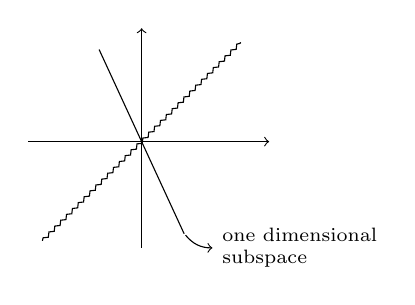
\begin{tikzpicture}[scale=0.9,baseline=(o.base)]
\coordinate (o) at (0,0);
\draw[->] (-1.6,0) -- (1.8,0);
\draw[->] (0,-1.5) -- (0,1.6);
% a line through the origin (steep, negative slope)
\draw (-0.6,1.3) -- (0.6,-1.3);
% one dimensional subspace: wavy line through the origin
\draw[decorate,decoration={snake,amplitude=0.6pt,segment length=3pt}] (-1.4,-1.4) -- (1.4,1.4);
\draw[->] (0.62,-1.32) to[bend right=25] (1.0,-1.5) node[right,align=left,font=\scriptsize] {one dimensional\\subspace};
\end{tikzpicture}
\qquad
$\begin{aligned}
\bmat{1\\1}&\in\W\\
-\bmat{1\\1}&\in\W
\end{aligned}
\qquad
a\odot x = 0_{\V} \ \text{ with } a=\0$
\end{center}
\explain{E.g.\ the line $\W=\Span\{(1,1)\T\}$ (the line $x_2=x_1$): with $(1,1)\T$ it also contains $-(1,1)\T$, and $\0\odot x=0_{\V}$ must lie in $\W$.}
\begin{itemize}[nosep]
\item \key{All subspaces should cross origin.}
\item For two dimensional subspace, include all $\R^2$.
\end{itemize}
\begin{insight}[Subspaces of $\R^2$]
The subspaces of $\R^2$ are exactly: $\{0_{\V}\}$ (dimension 0), every line through the origin (dimension 1), and $\R^2$ itself (dimension 2). A line not passing through the origin (such as $\{[a,\,1]\T\}$ above) is never a subspace.
\end{insight}

\begin{example}
$\V=\R^{2\times2}$, $\F=\R$, \quad $\W = \{\text{set of $2\times2$ real valued symmetric matrices}\}$
\begin{align*}
\bmat{a_1&b_1\\b_1&c_1}\oplus\bmat{a_2&b_2\\b_2&c_2} &= \bmat{a_1+a_2 & b_1+b_2\\ b_1+b_2 & c_1+c_2}\in\W\\
\alpha\bmat{a_1&b_1\\b_1&c_1} &= \bmat{\alpha a_1&\alpha b_1\\ \alpha b_1&\alpha c_1}\in\W
\end{align*}
$\therefore$ \key{$\W$ is a subspace of $\V$.}
\end{example}

\needspace{14\baselineskip}
\begin{example}
\begin{tabular}[t]{@{}l@{\ }l}
$\V$: & set of real valued functions defined over $\R$\\
$\W_1$: & set of real valued continuous functions\\
$\W_2$: & set of all real valued functions which are discontinuous at $t=1$
\end{tabular}

\needspace{11\baselineskip}
$\therefore$ $\W_1$ is a subspace. For $\W_2$:
\begin{center}
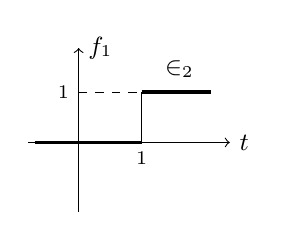
\begin{tikzpicture}[scale=0.8]
% f1: 0 for t<1, 1 for t>1
\draw[->] (-0.8,0) -- (2.4,0) node[right] {\small$t$};
\draw[->] (0,-1.1) -- (0,1.5) node[right] {\small$f_1$};
\draw[very thick] (-0.7,0) -- (1,0);
\draw[very thick] (1,0.8) -- (2.1,0.8);
\draw[thin] (1,0) -- (1,0.8);
\draw[dashed] (0,0.8) -- (1,0.8);
\node[left] at (0,0.8) {\scriptsize 1};
\node[below] at (1,0) {\scriptsize 1};
\node[below] at (1.6,1.45) {\small$\in\W_2$};
\end{tikzpicture}
\quad
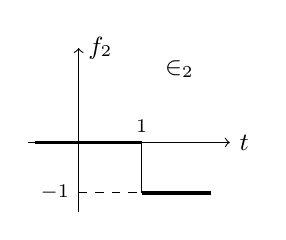
\begin{tikzpicture}[scale=0.8]
% f2: 0 for t<1, -1 for t>1
\draw[->] (-0.8,0) -- (2.4,0) node[right] {\small$t$};
\draw[->] (0,-1.1) -- (0,1.5) node[right] {\small$f_2$};
\draw[very thick] (-0.7,0) -- (1,0);
\draw[very thick] (1,-0.8) -- (2.1,-0.8);
\draw[thin] (1,0) -- (1,-0.8);
\draw[dashed] (0,-0.8) -- (1,-0.8);
\node[left] at (0,-0.8) {\scriptsize $-1$};
\node[above] at (1,0) {\scriptsize 1};
\node[below] at (1.6,1.45) {\small$\in\W_2$};
\end{tikzpicture}
\quad
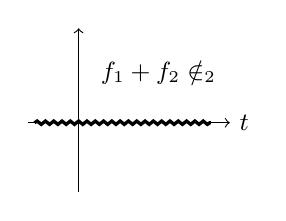
\begin{tikzpicture}[scale=0.8]
% f1+f2 = 0 (continuous)
\draw[->] (-0.8,0) -- (2.4,0) node[right] {\small$t$};
\draw[->] (0,-1.1) -- (0,1.5);
\draw[very thick,decorate,decoration={snake,amplitude=0.6pt,segment length=3pt}] (-0.7,0) -- (2.1,0);
\node[right] at (0.2,0.8) {\small$f_1+f_2\notin\W_2$};
\end{tikzpicture}
\end{center}
% corrected: the middle graph is labeled "\in W" in the notes; it is meant as \in W_2
\explain{$f_1$ and $f_2$ both jump at $t=1$, but $f_1+f_2$ is the zero function, which is continuous.}
$\therefore$ Not closed under vector addition \& scalar multiplication (multiply with zero: $0\cdot f_1$ is the zero function, which is continuous, so $\notin\W_2$). 

Hence \key{$\W_2$ is \underline{not} a subspace.}
\begin{insight}
$\W_1$ is a subspace because sums and scalar multiples of continuous functions are continuous (and the zero function is continuous). $\W_2$ fails already the quick test: the zero vector of $\V$ (the zero function) is not in $\W_2$.
\end{insight}
\end{example}

% ===== Page 6 =====
\subsection{Sums, Intersections and Products of Subspaces}\label{ss:sums}
\begin{definition}
The\origpage{6} \term{sum} $Y+Z$ of two subsets $Y$ \& $Z$ of a linear space is the set of all vectors $y+z$ where $y\in Y$ and $z\in Z$.
\[ Y+Z \triangleq \{ y+z \mid y\in Y,\ z\in Z\} \]
\end{definition}

\begin{example}
$\V=\R^2$,
\[
Y = \left\{\bmat{a\\0} \;\middle|\; 2\le a\le3\right\}, \qquad
Z = \left\{\bmat{0\\b} \;\middle|\; 1\le b\le2\right\}
\]
\begin{center}
\begin{tikzpicture}[scale=0.8]
\draw[->] (-0.5,0) -- (4,0) node[below] {\small$y$};
\draw[->] (0,-1.2) -- (0,3) node[left] {\small$z$};
\fill[pattern=north east lines] (2,1) rectangle (3,2);
\draw (2,1) rectangle (3,2);
\node at (3.4,2.4) {\small$Y+Z$};
\draw[thick,decorate,decoration={snake,amplitude=0.7pt,segment length=3pt}] (0,1) -- (0,2);
\draw[thick,decorate,decoration={snake,amplitude=0.7pt,segment length=3pt}] (2,0) -- (3,0);
\draw[dashed] (0,1) -- (2,1); \draw[dashed] (0,2) -- (2,2);
\draw[dashed] (2,0) -- (2,1); \draw[dashed] (3,0) -- (3,1);
\draw[->] (0,0) -- (2.4,1.5);
\node[left] at (0,1) {\scriptsize1}; \node[left] at (0,2) {\scriptsize2};
\node[below] at (2,-0.1) {\scriptsize2}; \node[below] at (3,-0.1) {\scriptsize3};
\end{tikzpicture}
\end{center}
% lead-in and figure kept together (needspace has no effect inside the breakable example box)
\par\noindent\begin{minipage}{\linewidth}
\setlength{\parskip}{0.45em}
If instead $Y$ and $Z$ are two lines through the origin (subspaces), every vector $x$ can be decomposed as $x=y+z$ with $y\in Y$, $z\in Z$:
\begin{center}
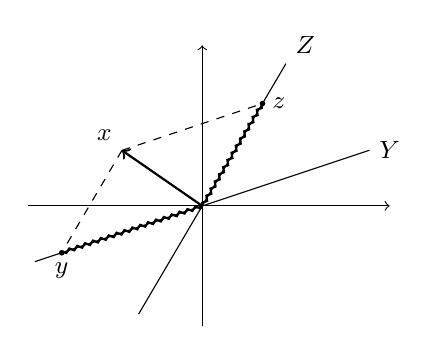
\begin{tikzpicture}[scale=0.85]
\draw[->] (-2.6,0) -- (2.8,0);
\draw[->] (0,-1.8) -- (0,2.4);
% Y: line through origin with slope 1/3, Z: line with slope 1.7
\draw (-2.5,-0.833) -- (2.5,0.833) node[right] {\small$Y$};
\draw (-0.95,-1.615) -- (1.25,2.125) node[above right] {\small$Z$};
% y in Y (negative direction), z in Z, x = y + z
\coordinate (y) at (-2.1,-0.7);
\coordinate (z) at (0.9,1.53);
\coordinate (x) at (-1.2,0.83);
\draw[thick,decorate,decoration={snake,amplitude=0.6pt,segment length=3pt}] (0,0) -- (y);
\draw[thick,decorate,decoration={snake,amplitude=0.6pt,segment length=3pt}] (0,0) -- (z);
\fill (y) circle (1.2pt) node[below] {\small$y$};
\fill (z) circle (1.2pt) node[right] {\small$z$};
\draw[->,thick] (0,0) -- (x) node[above left] {\small$x$};
\draw[dashed] (x) -- (z);
\draw[dashed] (x) -- (y);
\end{tikzpicture}
\end{center}
\end{minipage}\par
The same can be done for every vector, so $Y+Z = \R^2$ $\Rightarrow$ the sum of two subspaces is again a subspace.
\end{example}

\needspace{16\baselineskip}
\begin{remark}
If $Y$ \& $Z$ are both subspaces, then \key{$Y+Z$ is a subspace}.
\end{remark}
\begin{proof}
Let $x_1, x_2\in Y+Z$:
\begin{gather*}
x_1 = \underset{\in Y}{y_1}+\underset{\in Z}{z_1}, \qquad x_2 = \underset{\in Y}{y_2}+\underset{\in Z}{z_2}\\[6pt]
x_1+x_2 = y_1+z_1+y_2+z_2 = \underbrace{y_1+y_2}_{\in Y}+\underbrace{z_1+z_2}_{\in Z}
\end{gather*}
\explain{As $Y$ and $Z$ are subspaces, they are closed under addition.}
Similarly, for any scalar $\alpha$:
\[
\underbrace{\alpha x_1}_{\in Y+Z} = \alpha(y_1+z_1) = \underbrace{\alpha y_1}_{\in Y}+\underbrace{\alpha z_1}_{\in Z}
\]
Closed under scalar multiplication.

$\therefore$ $Y+Z$ is a subspace.
\end{proof}

\sep
For the two lines $Y$, $Z$ of the previous example:
\[ Y\cap Z = \left\{\bmat{0\\0}\right\} \text{ is a subspace} \Rightarrow \text{not a coincidence!} \]

\begin{remark}
If $Y$ \& $Z$ are subspaces, then \key{$Y\cap Z$ is a subspace}.

($Y\cup Z$ is closed under scalar multiplication but not closed under addition, which is the case in the previous example) $\Rightarrow$ \key{$Y\cup Z$ is not a subspace \underline{generally}}.
% corrected: notes had "Y u Z is not closed under addition but not closed under scalar multiplication"; Y u Z is always closed under scalar multiplication
\end{remark}
\begin{insight}
\begin{proof}[Proof for $Y\cap Z$]
If $x_1,x_2\in Y\cap Z$, then $x_1+x_2\in Y$ and $x_1+x_2\in Z$ (both are subspaces), so $x_1+x_2\in Y\cap Z$; similarly $\alpha x_1\in Y\cap Z$.
\end{proof}
\paragraph{Why $Y\cup Z$ fails.} For the two lines, $y\in Y$, $z\in Z$ nonzero give $y+z$, which lies on neither line. In fact $Y\cup Z$ is a subspace only if $Y\subseteq Z$ or $Z\subseteq Y$. The sum $Y+Z$ is the \key{smallest subspace containing $Y\cup Z$}.
\end{insight}

\begin{definition}[Product space]
Let $(\V,\F)$ \& $(\W,\F)$ be two linear spaces defined over the same field $\F$. The \term{product} of $(\V,\F)$ \& $(\W,\F)$ is defined as:
\begin{align*}
\V\times\W &= \{(v,w) \mid v\in\V,\ w\in\W\}\\
(v_1,w_1)\oplus_{\V\times\W}(v_2,w_2) &= (v_1\oplus_{\V} v_2,\; w_1\oplus_{\W} w_2)\\
\alpha\odot_{\V\times\W}(v_1,w_1) &= (\alpha\odot_{\V} v_1,\; \alpha\odot_{\W} w_1)
\end{align*}
% corrected: notes had w_1 \oplus_V w_2 and \alpha \odot_V w_1; the second components use the operations of W
\[
\Rightarrow\quad
(\underset{\V\times\W}{\R^2},\underset{\F}{\R}) = (\underset{\V}{\R},\underset{\F}{\R})\times(\underset{\W}{\R},\underset{\F}{\R})
\]
\end{definition}
\explain{In general $\dim(\V\times\W)=\dim\V+\dim\W$; e.g.\ $\R^n\times\R^m=\R^{n+m}$.}

% ===== Page 7 =====
\subsection{Linear Combinations, Span and Linear Independence}\label{ss:span-li}
\begin{definition}
A\origpage{7} \term{linear combination} of $n$ vectors $x_1,x_2,\dots,x_n$ of a linear space $\V$ is a vector of the form
\[ a_1x_1+a_2x_2+\dots+a_nx_n = \sum_{i=1}^{n} a_ix_i \qquad \text{where } a_i\in\F \text{ for } i=1,\dots,n \]
The set of all linear combinations of $x_1,\dots,x_n$, i.e.
\[ \left\{ \sum_{i=1}^{n} a_ix_i \;\middle|\; a_i\in\F,\ i=1,\dots,n \right\} \]
is called the \term{span} of $\{x_1,\dots,x_n\}$, denoted $\Span\{x_1,\dots,x_n\}$.
\end{definition}

For $\V=\R^2$:
\begin{align*}
&x_1=\bmat{1\\0},\ x_2=\bmat{0\\1}: && a_1\bmat{1\\0}+a_2\bmat{0\\1} = \bmat{a_1\\a_2} &&\Rightarrow\ \Span\{x_1,x_2\}=\R^2\\
&x_1=\bmat{1\\0},\ x_2=\bmat{0\\1},\ x_3=\bmat{1\\1}: && && \Rightarrow\ \Span\{x_1,x_2,x_3\}=\R^2
\end{align*}
\explain{$x_3$ is redundant: $x_3=x_1+x_2$ is already a linear combination of $x_1,x_2$, so adding it does not enlarge the span.}

\begin{definition}
Vectors $x_1,\dots,x_n\in\V$ are said to be \term{linearly independent} if and only if
\[ a_1x_1+a_2x_2+\dots+a_nx_n = 0_{\V} \quad\text{implies}\quad a_1=a_2=\dots=a_n=\0 \]
If $\exists\, a_1,\dots,a_n$, not all equal to $\0$, such that
\[ a_1x_1+\dots+a_nx_n = 0_{\V}, \]
then $x_1,x_2,\dots,x_n$ are \term{linearly dependent}.
\end{definition}

\begin{example}
$x_1=\bmat{1\\0}$, $x_2=\bmat{0\\1}$:
\[
a_1\bmat{1\\0}+a_2\bmat{0\\1} = \bmat{0\\0} = \bmat{a_1\\a_2}
\quad\Rightarrow\quad a_1=a_2=0 \quad\Rightarrow\quad \text{linearly independent}
\]
\end{example}

\begin{example}
$x_1=\bmat{1\\0}$, $x_2=\bmat{0\\1}$, $x_3=\bmat{1\\1}$:
\[
a_1\bmat{1\\0}+a_2\bmat{0\\1}+a_3\bmat{1\\1} = \bmat{0\\0}
\ \Rightarrow\
\begin{aligned} a_1+a_3&=0\\ a_2+a_3&=0 \end{aligned}
\ \Rightarrow\
\text{e.g.\ } a_1=a_2=1,\ a_3=-1
\]
$\therefore$ \key{Linearly dependent.}
\end{example}

\begin{example}
Consider the linear space of polynomials of degree $n\le2$, and
\[
P_1(t)=1, \quad P_2(t)=1+t, \quad P_3(t)=1+t+t^2, \qquad P=\{P_1(t),P_2(t),P_3(t)\}.
\]
Is $P$ linearly independent?
\begin{align*}
& a_1\cdot1+a_2(1+t)+a_3(1+t+t^2) = 0(t) && (\text{zero polynomial})\\
\Rightarrow\ & (a_1+a_2+a_3)+(a_2+a_3)t+a_3t^2 = 0(t) \ \Rightarrow\ a_1=a_2=a_3=0
\end{align*}
\explain{A polynomial is the zero polynomial only if all its coefficients vanish: $a_3=0$ (from $t^2$), then $a_2+a_3=0\Rightarrow a_2=0$ (from $t$), then $a_1+a_2+a_3=0\Rightarrow a_1=0$.}
$\therefore$ \key{$P$ is linearly independent.}
\end{example}

% ===== Page 8 =====
\needspace{12\baselineskip}
\begin{example}
$\V$:\origpage{8} set of all continuous functions defined over the real line.
\[ S = \left\{ \cos t,\ \sin t,\ \cos\!\left(t-\tfrac{\pi}{3}\right) \right\}. \quad \text{Is $S$ linearly independent?} \]
\[
a\cos t+b\sin t+c\,
\underbrace{\cos\!\left(t-\tfrac{\pi}{3}\right)}_{\cos t\,\cdot\,\cos\frac{\pi}{3}\;+\;\sin t\,\cdot\,\sin\frac{\pi}{3}} = 0(t)\quad \forall t,
\qquad \cos\tfrac{\pi}{3} = \tfrac12,\quad \sin\tfrac{\pi}{3} = \tfrac{\sqrt3}{2}
\]
Collecting terms:
\[ \left(a+\tfrac{c}{2}\right)\cos t+\left(b+\tfrac{\sqrt3}{2}c\right)\sin t = 0(t), \]
which holds for $a=-\tfrac{c}{2}$, $b=-\tfrac{\sqrt3}{2}c$ with any $c$. Choosing $a=-\tfrac12$, $b=-\tfrac{\sqrt3}{2}$, $c=1$ gives the zero function.

$\therefore$ \key{$S$ is \underline{not} linearly independent.}
\end{example}

\sep
Linear independence of the columns of a matrix $A = [c_1 \mid c_2 \mid \dots \mid c_n]$: consider $Ax=0$, i.e.
\[
[c_1 \mid c_2 \mid \dots \mid c_n]\bmat{x_1\\x_2\\\vdots\\x_n}
= \underbrace{c_1x_1+c_2x_2+\dots+c_nx_n}_{\text{zero}} = \bmat{0\\0\\\vdots\\0}
\]
\explain{$Ax$ is a linear combination of the columns of $A$ with coefficients $x_i$. Hence: \key{the columns $c_1,\dots,c_n$ are linearly independent $\iff$ $Ax=0$ has only the solution $x=0$}; any nonzero solution $x$ gives a dependence relation among the columns.}

\subsection{Basis, Dimension and Coordinates}\label{ss:basis}
\begin{definition}
Let $\V$ be a linear space and set of vectors $B=\{x_1,\dots,x_n\}$ be a subset of $\V$. $B$ is said to be a \term{basis} for $\V$ if and only if
\begin{enumerate}[label=(\roman*)]
\item $\Span B=\V$, and
\item $B$ is a linearly independent set.
\end{enumerate}
\end{definition}

For $\R^2$:
\begin{align*}
B_1 &= \left\{\bmat{1\\1}\right\} && \times\ \text{not a basis}\\
B_2 &= \left\{\bmat{1\\1},\bmat{1\\-1}\right\} && \checkmark\\
B_3 &= \left\{\bmat{1\\1},\bmat{1\\-1},\bmat{0\\1}\right\} && \times\ \text{not linearly independent}\\
B_4 &= \left\{\bmat{0\\1},\bmat{1\\0}\right\} && \checkmark\\
B_5 &= \left\{\bmat{1\\0},\bmat{1\\1}\right\} && \checkmark
\end{align*}
\explain{The two basis vectors should not be on the same line through the origin (their spans intersect only at the origin); there are infinitely many bases and the number of vectors is always 2.}
\explain{E.g.\ for $B_3$: $(0,1)\T=\tfrac12(1,1)\T-\tfrac12(1,-1)\T$. For $B_1$: $\Span B_1$ is only the line $x_2=x_1$, not $\R^2$.}

\begin{remark}
There are infinitely many basis sets for a linear space. \key{All of these basis sets have the same number of elements.} That number is called \term{dimension} of $\V$. If the dimension is finite, $\V$ is said to be \term{finite dimensional}. Otherwise, $\V$ is \term{infinite dimensional}.
\end{remark}

\begin{example}
$\V$ is the set of $2\times2$ real valued symmetric matrices:
\begin{gather*}
\bmat{a&b\\b&c} = a\bmat{1&0\\0&0}+b\bmat{0&1\\1&0}+c\bmat{0&0\\0&1}\\
B = \left\{ \bmat{1&0\\0&0},\bmat{0&1\\1&0},\bmat{0&0\\0&1} \right\}
\end{gather*}
\explain{3 elements (dimension 3).}
\point Infinite dimensional linear space $\Rightarrow$ set of continuous functions.
\explain{For every $n$, the functions $1,t,t^2,\dots,t^n$ are continuous and linearly independent, so no finite set can span this space.}
\end{example}

% ===== Page 9 =====
\begin{definition}
If\origpage{9} $y\in\V$ and $B=\{x_1,x_2,\dots,x_n\}$ is a basis set for $\V$, then there is a \key{unique} $n$-tuple of scalars $(a_1,a_2,\dots,a_n)$ such that
\[ y = \sum_{i=1}^{n} a_ix_i \]
The scalars $(a_1,a_2,\dots,a_n)$ are called \term{components} (\term{coordinates}), \term{representations} of $y$ with respect to (w.r.t.) basis $B$. We denote the representation of $y$ w.r.t.\ $B$ by $[y]_B$.
\end{definition}
With $B$ the basis of symmetric matrices above:
\[
y = \bmat{1&2\\2&3}\in\V, \qquad [y]_B = \underset{\substack{\uparrow\\\text{unique}}}{\bmat{1\\2\\3}}, \qquad y\in\V, \quad [y]_B\in\R^3
\]

\point Why should representation be unique?
\begin{proof}[Proof (by contradiction)]
$[y]_B$ is unique.

Suppose $[y]_B$ is \underline{not} unique:
\[
[y]_B = \bmat{\alpha_1\\\alpha_2\\\vdots\\\alpha_n}, \qquad [y]_B = \bmat{\beta_1\\\beta_2\\\vdots\\\beta_n}, \qquad \exists\, i \text{ such that } \alpha_i\neq\beta_i
\]
By the representation definition,
\[
y = \sum_{i=1}^{n}\alpha_ix_i, \qquad y=\sum_{i=1}^{n}\beta_ix_i
\qquad\Rightarrow\qquad
0_{\V} = \sum_{i=1}^{n}(\alpha_i-\beta_i)x_i
\]
\explain{A linear combination of the basis vectors equal to zero with some of the coefficients nonzero, as $\alpha_i-\beta_i\neq0$.}
% corrected: notes had "some of the vectors are nonzero"; it is the coefficients alpha_i - beta_i that are nonzero
$\therefore$ $x_i$ are linearly dependent $\Rightarrow$ contradiction.
\end{proof}

\begin{example}
$\V = \Span\{\cos t,\sin t\}$, \quad $B = \{\cos t,\sin t\}$
\[
y \triangleq \cos\!\left(t-\tfrac{\pi}{3}\right) = \tfrac12\cos t+\tfrac{\sqrt3}{2}\sin t
\qquad\Rightarrow\qquad [y]_B = \bmat{1/2\\\sqrt3/2}
\]
\end{example}

\subsection{Change of Basis}\label{ss:change-basis}
\begin{theorem}[Change of basis]
Let $\V$ be an $n$-dimensional linear space over $\R$. Let $B_1$ and $B_2$ be two basis sets for $\V$. Then, there exists an $n\times n$ \key{real invertible matrix $P$} such that
\[ [v]_{B_1} = P\,[v]_{B_2} \quad \forall v\in\V \]
\end{theorem}
\begin{center}
\begin{minipage}{0.5\textwidth}
\begin{gather*}
B_1 = \left\{\bmat{1\\0},\bmat{0\\1}\right\}, \qquad B_2 = \left\{\bmat{1\\1},\bmat{1\\-1}\right\}\\[4pt]
v = \alpha_1\bmat{1\\0}+\alpha_2\bmat{0\\1}\\[4pt]
[v]_{B_1} = \bmat{\alpha_1\\\alpha_2}, \qquad
[v]_{B_2} = \bmat{\alpha_1'\\\alpha_2'}
\end{gather*}
\end{minipage}\hfill
\begin{minipage}{0.42\textwidth}
\centering
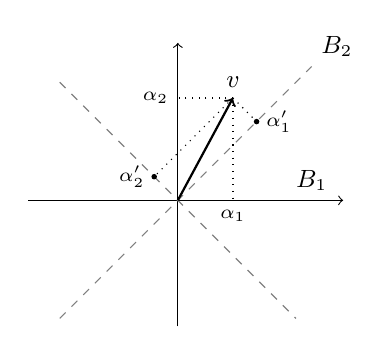
\begin{tikzpicture}[scale=1.0]
\draw[->] (-1.9,0) -- (2.1,0);
\draw[->] (0,-1.6) -- (0,2.0);
\node[above] at (1.7,0) {\small$B_1$};
% B_2 axes: y = x and y = -x
\draw[dashed,gray] (-1.5,-1.5) -- (1.7,1.7) node[above right,black] {\small$B_2$};
\draw[dashed,gray] (-1.5,1.5) -- (1.5,-1.5);
% v = (0.7,1.3) = 1.0*(1,1) - 0.3*(1,-1)
\draw[->,thick] (0,0) -- (0.7,1.3) node[above] {\small$v$};
\draw[dotted] (0.7,1.3) -- (0.7,0) node[below] {\scriptsize$\alpha_1$};
\draw[dotted] (0.7,1.3) -- (0,1.3) node[left] {\scriptsize$\alpha_2$};
\draw[dotted] (0.7,1.3) -- (1.0,1.0);
\draw[dotted] (0.7,1.3) -- (-0.3,0.3);
\fill (1.0,1.0) circle (1pt) node[right] {\scriptsize$\alpha_1'$};
\fill (-0.3,0.3) circle (1pt) node[left] {\scriptsize$\alpha_2'$};
\end{tikzpicture}
\end{minipage}
\end{center}
\begin{insight}[Finding $P$ for this example]
Write $v$ in terms of $B_2$:
\[ v=\alpha_1'\bmat{1\\1}+\alpha_2'\bmat{1\\-1}=\bmat{1&1\\1&-1}\bmat{\alpha_1'\\\alpha_2'}. \]
Since the $B_1$-coordinates are just the entries of $v$,
\[
[v]_{B_1}=\underbrace{\bmat{1&1\\1&-1}}_{P}[v]_{B_2},
\qquad
P^{-1}=\frac12\bmat{1&1\\1&-1}.
\]
In general, \key{the $j$-th column of $P$ is $[\,j\text{-th vector of }B_2\,]_{B_1}$}. $P$ is invertible because its columns are coordinates of a basis, hence linearly independent. For the drawn vector $v=(0.7,1.3)\T$: $[v]_{B_2}=P^{-1}[v]_{B_1}=(1,-0.3)\T$.
\end{insight}

\needspace{16\baselineskip}
\begin{example}
Consider $\V$: polynomials with degree $n\le2$.
\[
B_1 = \{\overset{v_1}{1},\ \overset{v_2}{1+t},\ \overset{v_3}{1+t+t^2}\},
\qquad
B_2 = \{\overset{w_1}{1},\ \overset{w_2}{t},\ \overset{w_3}{t^2}\}
\]
Find $P$ such that $[v]_{B_1} = P\,[v]_{B_2}$ $\forall v\in\V$.
% ===== Page 10 =====
\origpage{10}
\begin{align*}
v=w_1:&\quad [w_1]_{B_2} = \bmat{1\\0\\0} \Rightarrow P\bmat{1\\0\\0} = \text{1st column of } P = [w_1]_{B_1} = \bmat{1\\0\\0}\\[4pt]
v=w_2:&\quad [w_2]_{B_2} = \bmat{0\\1\\0} \Rightarrow P\bmat{0\\1\\0} = \text{2nd column of } P = [w_2]_{B_1} = \bmat{-1\\1\\0}\\[4pt]
v=w_3:&\quad [w_3]_{B_2} = \bmat{0\\0\\1} \Rightarrow P\bmat{0\\0\\1} = \text{3rd column of } P = [w_3]_{B_1} = \bmat{0\\-1\\1}
\end{align*}
% corrected: notes had "P = [w_1]_{B_1}", "P = [w_2]_{B_1}" (subscript hard to read) and "P . [w_3]_{B_2}" on the right; each is the corresponding column of P, i.e. [w_j]_{B_1}
\explain{The coordinates come from writing $B_2$ in terms of $B_1$: $w_1=1=v_1$, \ $w_2=t=(1+t)-1=v_2-v_1$, \ $w_3=t^2=(1+t+t^2)-(1+t)=v_3-v_2$.} Collecting the three columns:
\[
P = \bmat{1&-1&0\\0&1&-1\\0&0&1}
\]
\explain{Upper triangular matrix with diagonal entries 1. The diagonal entries are the eigenvalues $\Rightarrow$ $\det(P)$, the product of the eigenvalues, is $1\neq0$, so $P$ is invertible.}
In the opposite direction:
\[
[v]_{B_2} = Q\,[v]_{B_1} \ \Rightarrow\ Q = \bmat{1&1&1\\0&1&1\\0&0&1}, \qquad P = Q^{-1}
\]
\explain{Columns of $Q$ are $[v_j]_{B_2}$: $v_1=1$, $v_2=1+t$, $v_3=1+t+t^2$ give $(1,0,0)\T$, $(1,1,0)\T$, $(1,1,1)\T$.}
\begin{insight}[Check]
\[
PQ=\bmat{1&-1&0\\0&1&-1\\0&0&1}\bmat{1&1&1\\0&1&1\\0&0&1}=\bmat{1&0&0\\0&1&0\\0&0&1}.
\]
E.g.\ $v=3+2t+t^2$: $[v]_{B_2}=(3,2,1)\T$ and $P[v]_{B_2}=(1,1,1)\T$, i.e.\ $v=1\cdot1+1\cdot(1+t)+1\cdot(1+t+t^2)=3+2t+t^2$ \checkmark.
\end{insight}
\end{example}

% Section 2: Normed Vector Spaces  (original handwritten pages 11--18)
\section{Normed Vector Spaces}\label{sec:normed}
\syllabusweek{Week 3 --- normed spaces, sequences and convergence, matrix norms}

\subsection{Norms}\label{ss:norms}

\begin{definition}
Let $(\V,\F)$ be a vector space, a \term{norm} of $\V$ is a function shown as
\[ \norm{\cdot}: \V\to\R_{\ge0} \]
satisfying the following properties:
\begin{enumerate}[label=(N\arabic*),leftmargin=3.2em]
\item $\norm{v}\ge0 \quad \forall v\in\V$, \quad $\norm{v}=0 \iff v=0_{\V}$ \hfill (positive definiteness)
\item $\norm{\alpha v} = \abs{\alpha}\norm{v} \quad \forall v\in\V\ \&\ \forall\alpha\in\F$ \hfill (absolute homogeneity)
\item $\norm{v_1+v_2}\le\norm{v_1}+\norm{v_2} \quad \forall v_1,v_2\in\V$ \hfill (triangle inequality)
\end{enumerate}
The triplet $(\V,\F,\norm{\cdot})$ is called a \term{normed space}.
\end{definition}
\begin{align*}
&\norm{v} = \norm{v-0_{\V}}: && \text{size of } v\\
&\norm{v_1-v_2}: && \text{distance between } v_1 \ \&\ v_2
\end{align*}
We can define a sphere in $\V$:
\[
S = \{ v\in\V \mid \norm{v-v_0}\le r\} \qquad \text{sphere radius } r,\quad v_0: \text{center vector}
\]
\explain{Strictly, with ``$\le$'' this is the (closed) \term{ball}; the sphere is its boundary $\norm{v-v_0}=r$. The ``unit spheres'' drawn below are the sets $\norm{x}=1$.}

\begin{example}
$\V=\R^n$, $\F=\R$
\[
x = \bmat{x_1\\\vdots\\x_n}, \qquad \norm{x}_1 \overset{?}{=} \sum_{i=1}^{n}\abs{x_i}
\]
\paragraph{(N1).} $\abs{x_i}\ge0\ \forall i \Rightarrow \norm{x}_1\ge0$ \ $\checkmark$. \quad $0_{\V} = (0,\dots,0)\T$; if $\norm{x}_1=0$:
\[
\norm{x}_1 = \sum_{i=1}^{n}\abs{x_i} = 0
\ \Rightarrow\ \abs{x_i}=0 \ \forall i
\ \Rightarrow\ x=0_{\V}
\]
\paragraph{(N2).} $\alpha x = (\alpha x_1,\, \alpha x_2,\, \dots,\, \alpha x_n)\T$:
\begin{align*}
\norm{\alpha x}_1 &= \sum_{i=1}^{n}\abs{\alpha x_i} = \sum_{i=1}^{n}\abs{\alpha}\cdot\abs{x_i}
= \abs{\alpha}\cdot\underbrace{\sum_{i=1}^{n}\abs{x_i}}_{\norm{x}_1} = \abs{\alpha}\norm{x}_1
\end{align*}

% ===== Page 11 =====
\needspace{8\baselineskip}
\paragraph{(N3).} $x+y = (x_1+y_1,\, x_2+y_2,\, \dots,\, x_n+y_n)\T$:\origpage{11}
\begin{align*}
\norm{x+y}_1 = \sum_{i=1}^{n}\abs{x_i+y_i} &\le \sum_{i=1}^{n}\left(\abs{x_i}+\abs{y_i}\right)
= \underbrace{\sum_{i=1}^{n}\abs{x_i}}_{\norm{x}_1}+\underbrace{\sum_{i=1}^{n}\abs{y_i}}_{\norm{y}_1}
\end{align*}
% corrected: notes had \norm{x_i} in (1) and the sum without parentheses in (3)
\explain{The inequality uses the scalar triangle inequality $\abs{x_i+y_i}\le\abs{x_i}+\abs{y_i}$ term by term. Hence $\norm{x+y}_1\le\norm{x}_1+\norm{y}_1$ and all three properties hold: $\norm{\cdot}_1$ is a norm.}
\end{example}

\subsection{The $\ell_p$ Norms and Unit Spheres}\label{ss:lp}
\point $\norm{\cdot}_1$ is called \term{$\ell_1$ norm}.

\begin{example}[$\ell_2$ norm]
\[
\norm{x}_2 = \sqrt{\sum_{i=1}^{n}\abs{x_i}^2} = \left(\sum_{i=1}^{n}\abs{x_i}^2\right)^{1/2}
\]
Unit spheres for $x = (x_1,x_2)\T$: \ $\norm{x}_2=1$ and $\norm{x}_1 = 1$.

For $\ell_1$ norm: $\abs{x_1}+\abs{x_2}=1$
\begin{itemize}[nosep]
\item 1st quadrant ($x_1,x_2\ge0$): $x_1+x_2=1$
\item 2nd quadrant ($x_1\le0\le x_2$): $-x_1+x_2=1$
\item 3rd quadrant ($x_1,x_2\le0$): $-x_1-x_2=1$
\item 4th quadrant ($x_2\le0\le x_1$): $x_1-x_2=1$
\end{itemize}
% corrected: notes had "1st quadrant: x_1 - x_2 = 1"; in the 1st quadrant |x_1|+|x_2| = x_1+x_2. 3rd/4th quadrants added.
\explain{Four line segments joining $(\pm1,0)$ and $(0,\pm1)$: the $\ell_1$ unit sphere is a diamond (a square rotated by $45^\circ$), while the $\ell_2$ unit sphere $x_1^2+x_2^2=1$ is the circle.}
\begin{center}
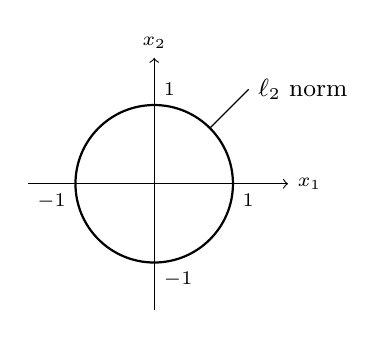
\begin{tikzpicture}[scale=1.0]
\draw[->] (-1.6,0) -- (1.7,0) node[right] {\scriptsize$x_1$};
\draw[->] (0,-1.6) -- (0,1.6) node[above] {\scriptsize$x_2$};
\draw[thick] (0,0) circle (1);
\node[below left] at (-1,0) {\scriptsize$-1$};
\node[below right] at (1,0) {\scriptsize$1$};
\node[above right] at (0,1) {\scriptsize$1$};
\node[below right] at (0,-1) {\scriptsize$-1$};
\draw (0.707,0.707) -- (1.2,1.2) node[right] {\small$\ell_2$ norm};
\end{tikzpicture}
\qquad\qquad
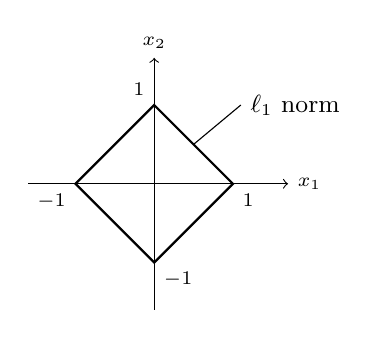
\begin{tikzpicture}[scale=1.0]
\draw[->] (-1.6,0) -- (1.7,0) node[right] {\scriptsize$x_1$};
\draw[->] (0,-1.6) -- (0,1.6) node[above] {\scriptsize$x_2$};
\draw[thick] (1,0) -- (0,1) -- (-1,0) -- (0,-1) -- cycle;
\node[below left] at (-1,0) {\scriptsize$-1$};
\node[below right] at (1,0) {\scriptsize$1$};
\node[above left] at (0,1) {\scriptsize$1$};
\node[below right] at (0,-1) {\scriptsize$-1$};
\draw (0.5,0.5) -- (1.1,1.0) node[right] {\small$\ell_1$ norm};
\end{tikzpicture}
\end{center}
\end{example}

\paragraph{$\ell_p$ norm.} The \term{$\ell_p$ norm} is
\[
\norm{x}_p = \left(\sum_{i=1}^{n}\abs{x_i}^p\right)^{1/p} \quad\text{where } p\ge1
\]
\paragraph{$\ell_\infty$ norm.} The \term{$\ell_\infty$ norm} is
\[
\norm{x}_\infty = \max_i\abs{x_i} = \lim_{p\to\infty}\norm{x}_p
\]
\needspace{9\baselineskip}
For $\V=\R^2$: $x=(x_1,x_2)\T$, \ $\norm{x}_p = \left(\abs{x_1}^p+\abs{x_2}^p\right)^{1/p}$. For $x_1=2$ \& $x_2=3$:
\begin{align*}
\norm{\bmat{2\\3}}_p &= (2^p+3^p)^{1/p}\\
&= (3^p)^{1/p}\cdot\left(1+\left(\tfrac23\right)^p\right)^{1/p}\\
&= 3\left(1+\left(\tfrac23\right)^p\right)^{1/p}\\
\lim_{p\to\infty}\norm{\bmat{2\\3}}_p &= 3 = \max\left(\abs{x_1},\abs{x_2}\right) = \norm{\bmat{2\\3}}_\infty
\end{align*}
\explain{$\left(\tfrac23\right)^p\to0$, so the factor $\left(1+(\tfrac23)^p\right)^{1/p}\to1$. In general the largest $\abs{x_i}$ dominates the sum: $\max_i\abs{x_i}\le\norm{x}_p\le n^{1/p}\max_i\abs{x_i}$ and $n^{1/p}\to1$.}

\sep
\point Unit spheres $\norm{x}_p=1$, i.e.\ $\norm{x-0_{\V}}_p=1$. The $\ell_\infty$ unit sphere is $\max(\abs{x_1},\abs{x_2}) = 1$.
\begin{center}
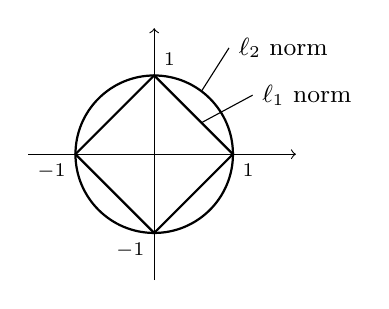
\begin{tikzpicture}[scale=1.0]
\draw[->] (-1.6,0) -- (1.8,0);
\draw[->] (0,-1.6) -- (0,1.6);
\draw[thick] (0,0) circle (1);
\draw[thick] (1,0) -- (0,1) -- (-1,0) -- (0,-1) -- cycle;
\node[below left] at (-1,0) {\scriptsize$-1$};
\node[below right] at (1,0) {\scriptsize$1$};
\node[above right] at (0,1) {\scriptsize$1$};
\node[below left] at (0,-1) {\scriptsize$-1$};
\draw (0.6,0.8) -- (0.95,1.35) node[right] {\small$\ell_2$ norm};
\draw (0.6,0.4) -- (1.25,0.75) node[right] {\small$\ell_1$ norm};
\end{tikzpicture}
\qquad\qquad
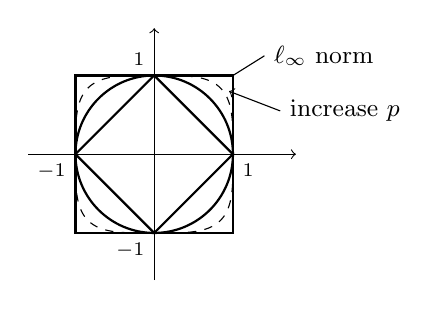
\begin{tikzpicture}[scale=1.0]
\draw[->] (-1.6,0) -- (1.8,0);
\draw[->] (0,-1.6) -- (0,1.6);
\draw[thick] (-1,-1) rectangle (1,1);
\draw[thick] (0,0) circle (1);
\draw[thick] (1,0) -- (0,1) -- (-1,0) -- (0,-1) -- cycle;
% intermediate p (p = 4): |x1|^4 + |x2|^4 = 1
\draw[dashed,domain=0:360,samples=145,smooth,variable=\t]
  plot ({sign(cos(\t))*abs(cos(\t))^(0.5)},{sign(sin(\t))*abs(sin(\t))^(0.5)});
\node[below left] at (-1,0) {\scriptsize$-1$};
\node[below right] at (1,0) {\scriptsize$1$};
\node[above left] at (0,1) {\scriptsize$1$};
\node[below left] at (0,-1) {\scriptsize$-1$};
\draw (1,1) -- (1.4,1.25) node[right] {\small$\ell_\infty$ norm};
\draw[->] (1.6,0.55) node[right] {\small increase $p$} -- (0.95,0.8);
\end{tikzpicture}
\end{center}
\explain{Dashed curve: $\abs{x_1}^p+\abs{x_2}^p=1$ for an intermediate $p$ (drawn for $p=4$); as $p$ increases the unit sphere moves from the $\ell_2$ circle towards the $\ell_\infty$ square.}

\sep
For $p=1/2$:
\[
\norm{x}_{1/2} = \left(\abs{x_1}^{1/2}+\abs{x_2}^{1/2}\right)^2
\]
\explain{It satisfies (N1) \& (N2) but need not satisfy the triangle inequality (N3).}
\paragraph{Counterexample.}
\[
x=\bmat{9\\0}, \quad y=\bmat{0\\4}, \quad x+y=\bmat{9\\4}
\]
\begin{align*}
\norm{x+y}_{1/2} &= \left(\sqrt9+\sqrt4\right)^2 = 25\\
\norm{x}_{1/2}&=9, \qquad \norm{y}_{1/2}=4\\
\norm{x+y}_{1/2} &\not\le \norm{x}_{1/2}+\norm{y}_{1/2}
\end{align*}
\[ \key{$p<1 \ \Rightarrow\ \text{no norms!}$} \]
\explain{Here $25>9+4=13$. Geometrically, for $p<1$ the ``unit sphere'' $\abs{x_1}^p+\abs{x_2}^p=1$ is star-shaped (curved inwards) and the unit ball is not convex; \key{a norm's unit ball is always convex}.}

% ===== Page 12 =====
\subsection{Norms on Function Spaces}\label{ss:function-norms}
\begin{center}\origpage{12}
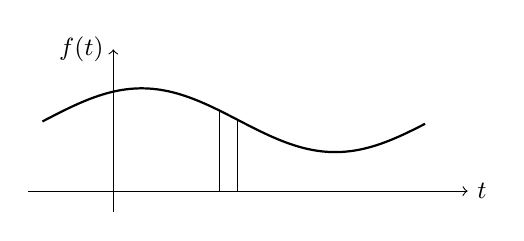
\begin{tikzpicture}[scale=0.9]
\draw[->] (-1.2,0) -- (5,0) node[right] {\small$t$};
\draw[->] (0,-0.3) -- (0,2) node[left] {\small$f(t)$};
\draw[thick,smooth,domain=-1:4.4,samples=60] plot (\x,{1.0+0.45*cos(deg(1.15*(\x-0.4)))});
% thin strip under the curve
\draw (1.5,0) -- (1.5,{1.0+0.45*cos(deg(1.15*1.1))});
\draw (1.75,0) -- (1.75,{1.0+0.45*cos(deg(1.15*1.35))});
\end{tikzpicture}
\end{center}
\[
\mathcal{L}_p = \left\{ f(\cdot) \;\middle|\; f:\R\to\R \text{ such that } \int_{-\infty}^{\infty}\abs{f(t)}^p\,dt<\infty \right\}, \qquad 1\le p<\infty
\]
\needspace{10\baselineskip}
\begin{align*}
\norm{f(t)}_p &= \left(\int_{-\infty}^{\infty}\abs{f(t)}^p\,dt\right)^{1/p} && \mathcal{L}_p \text{ norm}\\
\norm{f(t)}_1 &= \int_{-\infty}^{\infty}\abs{f(t)}\,dt && \mathcal{L}_1 \text{ norm}\\
\norm{f(t)}_2 &= \left(\int_{-\infty}^{\infty}\abs{f(t)}^2\,dt\right)^{1/2} && \mathcal{L}_2 \text{ norm}\\
\norm{f(t)}_\infty &= \sup_t\abs{f(t)} && \mathcal{L}_\infty \text{ norm}
\end{align*}
% corrected: notes had the L_p and L_2 integrals without dt, the L_1 norm without subscript, and max_t |f(t)| for L_infinity; the example below shows why sup is needed
\explain{These are the continuous analogues of the $\ell_p$ norms: the sum over $i$ becomes an integral over $t$.}

\sep
\needspace{12\baselineskip}
\begin{center}
$f(t) = 1-e^{-t},\quad t\ge0$
\qquad
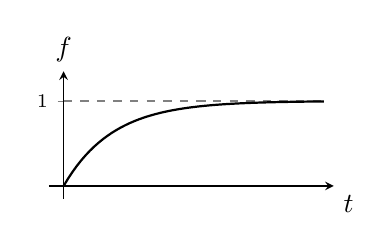
\begin{tikzpicture}[baseline=0.4cm]
\begin{axis}[width=5.2cm,height=3.2cm,axis lines=middle,xmin=-0.3,xmax=5.5,ymin=-0.15,ymax=1.35,
  xtick=\empty,ytick={1},xlabel={$t$},ylabel={$f$},
  xlabel style={anchor=north west},ylabel style={anchor=south},tick label style={font=\scriptsize}]
\addplot[dashed,gray,domain=0:5.3] {1};
\addplot[thick,domain=0:5.3,samples=60] {1-exp(-x)};
\end{axis}
\end{tikzpicture}
\end{center}
\explain{Value 1 is never reached. A maximum would have to be attained at a finite $t$, so $\max_t\abs{f(t)}$ does not exist here.}
The supremum, however, does exist:
\[ \sup_t\abs{f(t)} = 1 \quad (\text{least upper bound}) \]
\explain{Therefore \key{$\norm{f}_\infty$ is defined with $\sup$} (it always exists for bounded $f$), which equals $\max$ whenever the maximum is attained.}

\sep
\key{Integral norms do not satisfy $\norm{x}=0 \iff x=0_{\V}$!}
\begin{center}
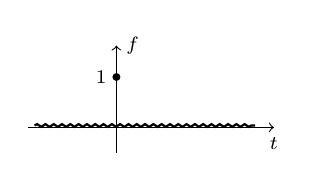
\begin{tikzpicture}[scale=0.8,baseline=0.2cm]
\draw[->] (-1.4,0) -- (2.5,0) node[below] {\scriptsize$t$};
\draw[->] (0,-0.4) -- (0,1.3) node[right] {\scriptsize$f$};
\fill (0,0.8) circle (1.8pt);
\node[left] at (0,0.8) {\scriptsize1};
\draw[thick,decorate,decoration={snake,amplitude=0.5pt,segment length=3pt}] (-1.3,0.03) -- (2.2,0.03);
\end{tikzpicture}
\qquad
$f(t) = \begin{cases} 1, & t=0\\ 0, & \text{otherwise}\end{cases}
\qquad\Rightarrow\qquad
\displaystyle\int_{-\infty}^{\infty}\abs{f(t)}\,dt = 0$
\end{center}
\explain{Such functions are equivalent to the zero function, as they take nonzero values only at finitely many points.}
\begin{insight}[How this is fixed]
$f\neq0$ but $\norm{f}_1=0$, so property (N1) fails on the set of all functions. The standard remedy: regard two functions as \emph{equal} in $\mathcal{L}_p$ if they differ only on a set of zero length (e.g.\ finitely many points), i.e.\ if $\norm{f-g}_p=0$. With this identification $\norm{\cdot}_p$ is a genuine norm on $\mathcal{L}_p$ for $p\ge1$ (the triangle inequality is Minkowski's inequality).
\end{insight}

\subsection{Matrix Norms}\label{ss:matrix-norms}
\[ A = \bmat{1&-2\\3&4}, \qquad \norm{A}=\,? \]

\subsubsection{Entrywise Norms (Frobenius)}
\needspace{14\baselineskip}
\paragraph{1st method.}
\[
\operatorname{Vec}(A) \triangleq \bmat{1\\3\\-2\\4}, \qquad A = \bmat{a_{11}&a_{12}\\a_{21}&a_{22}}
\]
\begin{align*}
\norm{A}_p = \norm{\operatorname{Vec}(A)}_p = \norm{\bmat{1\\3\\-2\\4}}_p &= \left(\abs{1}^p+\abs{3}^p+\abs{-2}^p+\abs{4}^p\right)^{1/p}\\
&= \left(\sum_{i,j}\abs{a_{ij}}^p\right)^{1/p}, \qquad p\ge1
\end{align*}
\begin{insight}[Numbers for this $A$]
\[
\norm{A}_1 = 1+2+3+4 = 10, \quad
\norm{A}_2 = \sqrt{1+4+9+16}=\sqrt{30}\approx5.48, \quad
\norm{A}_\infty = \max_{i,j}\abs{a_{ij}} = 4
\]
The case $p=2$ is the \term{Frobenius norm} $\norm{A}_F$. Since $\R^{m\times n}$ is a vector space that is identified with $\R^{mn}$ through $\operatorname{Vec}$, every vector norm gives a matrix norm in this way.
\end{insight}

% ===== Page 13 =====
\origpage{13}
\paragraph{1st method (Frobenius norm).}
% consistency: notes wrote ||A||_2 here; renamed ||A||_F as in the insight below (||A||_2 is reserved for the induced 2-norm)
\begin{align*}
\norm{A}_F &= \Big(\sum_{i,j} |a_{ij}|^2\Big)^{1/2} && \text{(\term{Frobenius norm})}\\
&= \sqrt{\tr(A\T A)} && \text{(real)}\\
&= \sqrt{\tr(A\Hm A)} && \text{(complex)}
\end{align*}
For example, with
\[
A = \bmat{a_{11} & a_{12}\\ a_{21} & a_{22}},
\qquad
A\T A = \underbrace{\bmat{a_{11} & a_{21}\\ a_{12} & a_{22}}}_{A\T}
\underbrace{\bmat{a_{11} & a_{12}\\ a_{21} & a_{22}}}_{A}
= \bmat{a_{11}^2 + a_{21}^2 & \\ & a_{12}^2 + a_{22}^2}
\]
% corrected: notes had tr(A) on the left-hand side (the trace taken is that of A^T A)
\needspace{5\baselineskip}
\begin{align*}
\tr(A\T A) &= a_{11}^2 + a_{21}^2 + a_{12}^2 + a_{22}^2\\*
&= \sum_{i,j} a_{ij}^2
\end{align*}
\explain{Only the diagonal of $A\T A$ matters for the trace, so its off-diagonal entries ($a_{11}a_{12}+a_{21}a_{22}$) are left blank.}
\begin{insight}
In general $(A\Hm A)_{jj} = \sum_i \overline{a_{ij}}\,a_{ij} = \sum_i |a_{ij}|^2$ is the squared length of the $j$-th column of $A$, so
$\tr(A\Hm A) = \sum_j\sum_i |a_{ij}|^2$. The Frobenius norm is simply the Euclidean norm of $A$ viewed as a long vector in $\F^{mn}$; we write it $\norm{A}_F$ to distinguish it from the \emph{induced} $2$-norm of the 2nd method below (which is in general different, e.g.\ $\norm{I_n}_F = \sqrt n$ but the induced norm of $I_n$ is $1$).
\end{insight}

\subsubsection{Induced Matrix Norms}
\paragraph{2nd method (induced norm).} Measure $A$ through its action on vectors.
\begin{definition}
Let $A:\R^n \to \R^m$ be an $m\times n$ matrix. Let $\norm{\cdot}_{\R^n}$ and $\norm{\cdot}_{\R^m}$ denote the norms in $\R^n$ \& $\R^m$ respectively. The \term{induced matrix norm} is defined as
\[
\norm{A} \triangleq \max_{\substack{x\in\R^n\\ x\neq 0_{\V}}} \frac{\norm{Ax}_{\R^m}}{\norm{x}_{\R^n}}
\]
\end{definition}
\[
\underbrace{\bmat{a_{11} & \cdots & a_{1n}\\ \vdots & \ddots & \vdots\\ a_{m1} & \cdots & a_{mn}}}_{A}
\underbrace{\bmat{x_1\\ \vdots\\ x_n}}_{x}
=
\underbrace{\bmat{y_1\\ \vdots\\ y_m}}_{y}
\]

\paragraph{Why second method?}
\begin{align*}
|\inner{x}{y}| &\le \norm{x}\norm{y}\\
\norm{Ax} &\le \norm{A}\norm{x}\\
\norm{Ax} &= \frac{\norm{Ax}}{\norm{x}}\cdot\norm{x} \le \left(\max\frac{\norm{Ax}}{\norm{x}}\right)\cdot\norm{x} = \norm{A}\norm{x}
\end{align*}
\explain{``Cauchy--Schwarz''-like inequality for matrices: \key{$\norm{Ax}\le\norm{A}\norm{x}$ for every $x$}.}
\begin{insight}[Why the induced norm is useful]
The induced norm is the largest ``gain'' $\norm{Ax}/\norm{x}$ of $A$, so $\norm{Ax}\le\norm{A}\norm{x}$ holds for every $x$ with the smallest possible constant. It is also submultiplicative: $\norm{ABx}\le\norm{A}\norm{Bx}\le\norm{A}\norm{B}\norm{x}$, hence $\norm{AB}\le\norm{A}\norm{B}$, which is what makes it convenient for bounding $\lVert A^k\rVert$ in system analysis.
\end{insight}

\begin{align*}
\norm{A} &= \max_{\substack{x\in\R^n\\ x\neq 0_{\V}}} \norm{A\frac{x}{\norm{x}_{\R^n}}}_{\R^m}\\
&= \max_{\norm{x}_{\R^n}=1} \norm{Ax}_{\R^m}
\end{align*}
\explain{First step: absolute homogeneity of the norm, $\frac{\norm{Ax}}{\norm{x}} = \norm{A\frac{x}{\norm{x}}}$, and $\frac{x}{\norm{x}}$ ranges over all unit vectors.}
\needspace{10\baselineskip}
\begin{keybox}
\[
\therefore\ \norm{A} = \max_{\norm{x}_{\R^n}=1} \norm{Ax}_{\R^m}
\]
\end{keybox}
\begin{center}
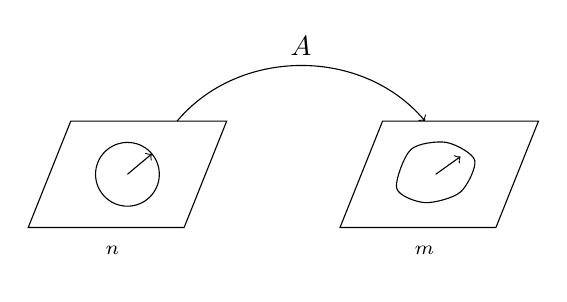
\begin{tikzpicture}[scale=0.9]
  % R^n parallelogram with unit ball
  \draw (0,0) -- (2.2,0) -- (2.8,1.5) -- (0.6,1.5) -- cycle;
  \draw (1.4,0.75) circle (0.45);
  \draw[->] (1.4,0.75) -- ++(40:0.45);
  \node at (1.2,-0.4) {$\R^n$};
  % R^m parallelogram with image of the unit ball
  \draw (4.4,0) -- (6.6,0) -- (7.2,1.5) -- (5.0,1.5) -- cycle;
  \draw plot[smooth cycle] coordinates {(5.2,0.55) (5.6,0.35) (6.1,0.5) (6.3,0.95) (5.9,1.2) (5.4,1.1)};
  \draw[->] (5.75,0.75) -- (6.1,1.0);
  \node at (5.6,-0.4) {$\R^m$};
  % mapping arrow
  \draw[->] (2.1,1.5) to[out=50,in=130] node[above] {$A$} (5.6,1.5);
\end{tikzpicture}
\end{center}

% ===== Page 14 =====
\origpage{14}
\begin{example}
Consider an $m\times n$ matrix with real elements. Choose $\ell_\infty$-norm $\norm{\cdot}_\infty$ for both $\R^n$ \& $\R^m$.
\[
\norm{A}_\infty = \max_{\norm{x}_\infty=1} \norm{Ax}_\infty,
\qquad
A = \bmat{1 & -2\\ -3 & 4\\ -2 & 2},
\qquad x\in\R^2,\quad y = Ax \in \R^3
\]
\[
\norm{x}_\infty = \max(|x_1|,|x_2|) = 1
\]
\begin{center}
\begin{minipage}{0.4\textwidth}
\centering
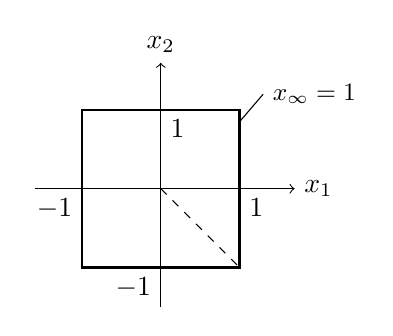
\begin{tikzpicture}[scale=1.0]
  \draw[->] (-1.6,0) -- (1.7,0) node[right] {$x_1$};
  \draw[->] (0,-1.5) -- (0,1.6) node[above] {$x_2$};
  \draw[thick] (-1,-1) rectangle (1,1);
  \node[below left] at (-1,0) {$-1$};
  \node[below right] at (1,0) {$1$};
  \node[below right] at (0,1) {$1$};
  \node[below left] at (0,-1) {$-1$};
  \draw[dashed] (0,0) -- (1,-1);
  \draw (1,0.85) -- (1.3,1.2) node[right,font=\small] {$\norm{x}_\infty=1$};
\end{tikzpicture}
\end{minipage}%
\begin{minipage}{0.55\textwidth}
First row only:
\[
A_1 = \bmat{1 & -2}\bmat{x_1\\ x_2}
\]
\[
\max_{\norm{x}_\infty=1} |A_1 x| = \max_{\norm{x}_\infty=1} |x_1 - 2x_2| = 3
\]
\explain{Attained at $x_1 = 1$, $x_2 = -1$ (dashed corner).}
\end{minipage}
\end{center}
For the whole matrix:
\begin{align*}
Ax &= \bmat{x_1 - 2x_2\\ -3x_1 + 4x_2\\ -2x_1 + 2x_2}\\
\norm{Ax}_\infty &= \max\big(|x_1 - 2x_2|,\ |-3x_1+4x_2|,\ |-2x_1+2x_2|\big)\\
x^* &= \bmat{1\\ -1} \quad\text{or}\quad x^* = \bmat{-1\\ 1}\\
Ax^* &= \bmat{3\\ -7\\ -4} \;\Rightarrow\; \norm{Ax^*}_\infty = 7
\end{align*}
\[
\boxed{\norm{A}_\infty = 7}
\]
\end{example}
\needspace{11\baselineskip}
\begin{keybox}
\[
\norm{A}_\infty = \max_i \sum_{j=1}^n |a_{ij}| \qquad \text{(max row sum)}
\]
\end{keybox}
\begin{insight}[Why the max row sum]
If $\norm{x}_\infty = 1$ then $|x_j|\le 1$ for all $j$, so for each row
$|(Ax)_i| = \big|\sum_j a_{ij}x_j\big| \le \sum_j |a_{ij}||x_j| \le \sum_j |a_{ij}|$.
Hence $\norm{Ax}_\infty\le\max_i\sum_j|a_{ij}|$. Equality is reached by taking the row $i^*$ with the largest sum and $x_j = \operatorname{sign}(a_{i^*j})$ (a corner of the square). In the example the row sums are $3,7,4$ and row 2 $= [-3\ \ 4]$ gives $x^* = [-1\ \ 1]\T$ (or its negative).
\end{insight}

\sep
\paragraph{$\ell_1$-norm.}
\[
\norm{A}_1 = \max_{\norm{x}_1=1}\norm{Ax}_1, \qquad \norm{x}_1 = |x_1| + |x_2| = 1
\]
\begin{center}
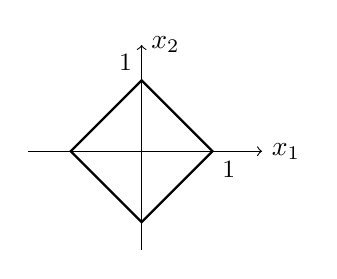
\begin{tikzpicture}[scale=0.9]
  \draw[->] (-1.6,0) -- (1.7,0) node[right] {$x_1$};
  \draw[->] (0,-1.4) -- (0,1.5) node[right] {$x_2$};
  \draw[thick] (1,0) -- (0,1) -- (-1,0) -- (0,-1) -- cycle;
  \node[below right,font=\small] at (1,0) {$1$};
  \node[above left,font=\small] at (0,1) {$1$};
\end{tikzpicture}
\end{center}
\begin{align*}
A_1 &= \bmat{1 & -2}\\
A_1 x &= x_1 - 2x_2\\
\norm{A_1 x} &= |x_1 - 2x_2|\\
\max_{\norm{x}_1 = 1}\norm{A_1 x} &= \max_{\norm{x}_1 = 1} |x_1 - 2x_2|
\end{align*}
\explain{Weighted average of $1$ and $-2$: on $\norm{x}_1=1$, $|x_1 - 2x_2| \le |x_1| + 2|x_2| \le 2(|x_1|+|x_2|) = 2$, so the best is to put all the weight on the entry of largest magnitude.}
\needspace{7\baselineskip}
\begin{align*}
x &= \bmat{0.5\\ -0.5} \quad\Rightarrow\quad \tfrac12 + 1 = \tfrac32\\
x &= \bmat{0.2\\ -0.8} \quad\Rightarrow\quad \text{larger}\\
x &= \bmat{0\\ -1} \quad\Rightarrow\quad \text{largest:}\quad \underline{\norm{A_1x} = 2}
\end{align*}

% ===== Page 15 =====
\origpage{15}
Now the whole matrix:
\[
A = \bmat{1 & -2\\ -3 & 4\\ -2 & 2}, \qquad
Ax = \bmat{1\\ -3\\ -2}x_1 + \bmat{-2\\ 4\\ 2}x_2
\]
\[
\norm{Ax}_1 = \Bigg\|\underbrace{\bmat{1\\ -3\\ -2}}_{6}x_1 + \underbrace{\bmat{-2\\ 4\\ 2}}_{8\ \checkmark}x_2\Bigg\|_1 = 8
\qquad (x_1 = 0,\ x_2 = 1)
\]
% corrected: notes have a stray "7" written below the "8"; the value of ||A||_1 is 8 (column sums 6 and 8); 7 is ||A||_inf from the previous page
\explain{Column sums: $|1|+|-3|+|-2| = 6$ and $|-2|+|4|+|2| = 8$, so $\norm{A}_1 = 8$ (compare $\norm{A}_\infty = 7$: different vector norms give different matrix norms).}
\needspace{9\baselineskip}
\begin{keybox}
\[
\norm{A}_1 = \max_j \sum_i |a_{ij}| \qquad \text{(max column sum)}
\]
\end{keybox}
\begin{insight}[Why the max column sum]
Write $A = [a_1\ \cdots\ a_n]$ by columns. If $\norm{x}_1 = 1$,
$\norm{Ax}_1 = \big\|\sum_j x_j a_j\big\|_1 \le \sum_j |x_j|\,\norm{a_j}_1 \le \big(\max_j\norm{a_j}_1\big)\sum_j|x_j| = \max_j\norm{a_j}_1$,
with equality for $x = e_{j^*}$ (a corner of the diamond), $j^*$ the column of largest absolute sum.
\end{insight}

\subsection{Convergence of Sequences}\label{ss:convergence}
\begin{definition}
Let $(\V,\F,\norm{\cdot})$ be a normed space. Let $\{v_n\}_{n=1}^\infty$ be a sequence of vectors in $\V$, i.e.\ $v_n\in\V\ \forall n$. The sequence $\{v_n\}_{n=1}^\infty$ is said to \term{converge} to the \term{limit} $\boxed{v\in\V}$ iff
\[
\boxed{\norm{v_n - v} \to 0 \quad \text{as } n\to\infty}
\]
\end{definition}
\begin{remark}
A sequence is \term{divergent} if it is not convergent.
\end{remark}
\begin{example}
$\V = \R$, $\norm{v} = |v|$.

\paragraph{Sequence $v_n = (1/2)^n$.} Candidate limit $v = 0 \in \V$:
\begin{align*}
\norm{v_n - v} &= \left|\frac{1}{2^n} - 0\right| = \frac{1}{2^n}\\
\lim_{n\to\infty}\norm{v_n - v} &= 0
\;\Rightarrow\; v_n \to 0 \text{ as } n\to\infty
\end{align*}

\paragraph{Sequence $v_n = (-1)^n$.} Try $v = 0$:
\[
\norm{(-1)^n - 0} = |(-1)^n| = 1, \qquad \lim_{n\to\infty}\overbrace{\norm{v_n - v}}^{1} = 1 \neq 0
\]
\explain{The sequence does not converge to $v = 0$.}
Try $v = 1$:
\[
\norm{(-1)^n - 1} = \abs{(-1)^n - 1} = \begin{cases} 0, & n \text{ even}\\ 2, & n \text{ odd}\end{cases} \;\Rightarrow\; \text{does not converge}
\]
% corrected: notes had ||(-1)^n - 1|| = (-1)^n - 1 (absolute value missing; that expression is negative for odd n)
\explain{The distance keeps jumping back to $2$, so it does not tend to $0$.}
$\therefore$ \key{Sequence is not convergent anywhere.}
\begin{insight}
For an arbitrary candidate $v\in\R$: the even terms are $1$ and the odd terms are $-1$, so by the triangle inequality $2 = |1-(-1)| \le |v_{2k}-v| + |v - v_{2k+1}|$. Thus at least one of two consecutive distances is $\ge 1$, and $\norm{v_n - v}\not\to 0$ for every $v$.
\end{insight}
\end{example}

\begin{example}
$\V = \left\{ f : [-1,1]\to\R \;\middle|\; f(\cdot) \text{ is continuous}, \ \int_{-1}^{1}|f(t)|\,dt < \infty \right\}$
\[
\norm{f(\cdot)} = \int_{-1}^{1} |f(t)|\,dt \qquad (\mathcal{L}_1 \text{ norm})
\]
% corrected: notes had the integral over (-infinity, infinity); functions in V live on [-1,1]
\needspace{7\baselineskip}
Is $f_n$ convergent?
\begin{align*}
f_n(t) &= e^{-n|t|}, \quad n\ge 0\\
f_0(t) &= e^{0t} = 1\\
f_1(t) &= e^{-|t|}\\
f_2(t) &= e^{-2|t|}\\
&\ \,\vdots
\end{align*}

% ===== Page 16 =====
\origpage{16}
\begin{center}
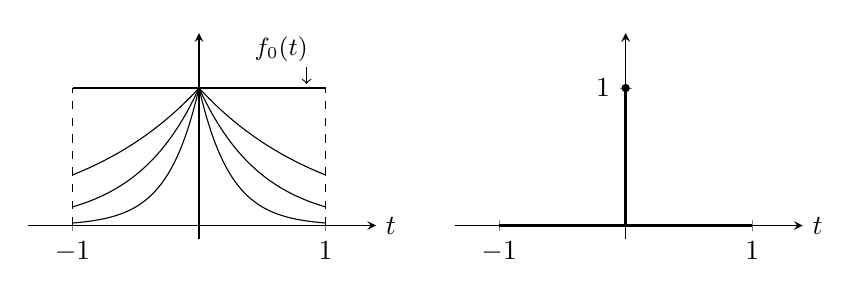
\begin{tikzpicture}
\begin{axis}[name=left,width=6cm,height=4.2cm,axis lines=middle,
  xmin=-1.35,xmax=1.4,ymin=-0.1,ymax=1.4,xtick={-1,1},ytick=\empty,
  xlabel={$t$},clip=false,every axis x label/.style={at={(current axis.right of origin)},anchor=west}]
  \addplot[thick,domain=-1:1] {1};
  \addplot[dashed] coordinates {(-1,0) (-1,1)};
  \addplot[dashed] coordinates {(1,0) (1,1)};
  \foreach \n in {1,2,4} {
    \addplot[domain=-1:1,samples=81] {exp(-\n*abs(x))};
  }
  \node[above,font=\small] at (axis cs:0.65,1.12) {$f_0(t)$};
  \draw[->] (axis cs:0.85,1.15) -- (axis cs:0.85,1.03);
\end{axis}
\begin{axis}[at={(left.east)},anchor=west,xshift=1cm,width=6cm,height=4.2cm,axis lines=middle,
  xmin=-1.35,xmax=1.4,ymin=-0.1,ymax=1.4,xtick={-1,1},ytick={1},
  xlabel={$t$},every axis x label/.style={at={(current axis.right of origin)},anchor=west}]
  \addplot[very thick] coordinates {(-1,0) (1,0)};
  \addplot[very thick] coordinates {(0,0) (0,1)};
  \addplot[only marks,mark=*,mark size=1.3pt] coordinates {(0,1)};
\end{axis}
\end{tikzpicture}
\end{center}
\explain{Left: $f_0, f_1, f_2, f_4$. Right: pointwise limit as $n\to\infty$ ($0$ for $t\neq0$, $1$ at $t=0$) $\notin \V$ (not continuous).}

\begin{center}
\begin{minipage}{0.32\textwidth}
\centering
\begin{tikzpicture}
\begin{axis}[width=4.6cm,height=3.2cm,axis lines=middle,
  xmin=-1.35,xmax=1.4,ymin=-0.3,ymax=1.2,xtick={-1,1},ytick=\empty]
  \addplot[very thick] coordinates {(-1,0) (1,0)};
\end{axis}
\end{tikzpicture}

$0(t)\in\V$
\end{minipage}%
\begin{minipage}{0.64\textwidth}
Candidate limit: the zero function $0(t)$.\\ $v\in\V$ is satisfied \checkmark
\end{minipage}
\end{center}
\begin{align*}
\norm{f_n(t) - 0(t)} &= \norm{f_n(t)} = \int_{-1}^{1}\left|e^{-n|t|}\right|dt\\
&= \int_{-1}^{1} e^{-n|t|}\,dt
&&\text{(exponential is positive)}\\
&= 2\cdot\int_0^1 e^{-nt}\,dt
&&\text{(even function)}\\
&= 2\,\frac{e^{-nt}}{-n}\bigg|_0^1 = -2\left(\frac{e^{-n}}{n} - \frac1n\right)\\
\norm{f_n(t) - 0(t)} &= -\frac{2}{n}\big(\underbrace{e^{-n} - 1}_{\to -1}\big) = \frac{2\,(1-e^{-n})}{n} \le \frac2n\\
\lim_{n\to\infty}\norm{f_n(t) - 0(t)} &= 0 \;\Rightarrow\; \norm{v_n - v}\to 0 \text{ as } n\to\infty \ \checkmark
\end{align*}
$\therefore$ \key{It is convergent to the zero function.}
\end{example}

\needspace{12\baselineskip}
\sep
\key{Convergence depends on the distance definition} (the norm):
\begin{itemize}[nosep]
\item for the $\mathcal{L}_1$ norm $\Rightarrow$ convergent
\item for the $\mathcal{L}_\infty$ (sup) norm $\Rightarrow$ divergent
\end{itemize}
\begin{insight}
With $\norm{f}_\infty = \max_{-1\le t\le 1}|f(t)|$ we get $\norm{f_n - 0}_\infty = \max_t e^{-n|t|} = 1$ (at $t=0$) for every $n$, so $f_n\not\to 0$. No other continuous $g$ works either: $\norm{f_n - g}_\infty\to0$ would force $g(t) = \lim_n f_n(t)$ pointwise, i.e.\ $g(0)=1$ and $g(t)=0$ for $t\neq0$, which is not continuous. The $\mathcal L_1$ norm only ``sees'' area, and the area under the narrowing peak vanishes; the $\mathcal L_\infty$ (sup) norm sees the peak height, which stays $1$.
\end{insight}

\subsection{Cauchy Sequences and Completeness}\label{ss:cauchy}
\begin{definition}
Let $(\V,\F,\norm{\cdot})$ be a normed space. A sequence $\{v_n\}_{n=0}^\infty$ is said to be a \term{Cauchy sequence} iff
\[
\lim_{n,m\to\infty}\norm{v_n - v_m} = 0
\]
\end{definition}
\begin{claim}
\key{Every convergent sequence is a Cauchy sequence.} The reverse statement, in general, is not correct.
\[
\text{Convergent} \;\underset{\not\Leftarrow}{\Rightarrow}\; \text{Cauchy}
\]
\end{claim}
\begin{proof}
Suppose that $\{v_n\}_{n=0}^\infty$ is convergent to $v\in\V$, i.e.\ $\lim_{n\to\infty}\norm{v_n - v} = 0$. Then
\begin{align*}
\lim_{n,m\to\infty}\norm{v_n - v_m} &= \lim_{n,m\to\infty}\norm{v_n - v + v - v_m}\\
&\le \lim_{n,m\to\infty} \big(\norm{v_n - v} + \norm{v - v_m}\big)\\
&= \underbrace{\lim_{n\to\infty}\norm{v_n - v}}_{=0} + \underbrace{\lim_{m\to\infty}\norm{v_m - v}}_{=0} = 0
\end{align*}
\explain{Inequality step: triangle inequality, $\norm{a+b}\le\norm{a}+\norm{b}$ with $a = v_n - v$, $b = v - v_m$.}
\[
0 \le \lim_{n,m\to\infty}\norm{v_n - v_m} \le 0 \;\Rightarrow\; \lim_{n,m\to\infty}\norm{v_n - v_m} = 0 \;\Rightarrow\; \{v_n\} \text{ is Cauchy.}
\qedhere
\]
\end{proof}
% corrected: notes justified the inequality step "by absolute convergence"; it is the triangle inequality (and ||v - v_m|| = ||v_m - v|| by homogeneity with alpha = -1)

% ===== Page 17 =====
\origpage{17}
\begin{example}
$\V = \Q$: set of rational numbers, $\F = \Q$ as well.
\[
\sqrt{2} = 1.41421356237310\ldots \;\Rightarrow\; \text{not a rational number}
\]
\begin{align*}
v_0 &= 1 = \tfrac11\\
v_1 &= 1.4 = \tfrac{14}{10}\\
v_2 &= 1.41 = \tfrac{141}{100}\\
v_3 &= 1.414 = \tfrac{1414}{1000}\\
&\ \,\vdots
\end{align*}
\needspace{7\baselineskip}
We need $v\in\V$ such that $\norm{v_n - v}\to 0$ as $n\to\infty$, where $v_n \in\V\ \forall n$.
But $v$ should be $\sqrt2$ for $\norm{v_n - v}\to 0$ as $n\to\infty$.
\begin{center}
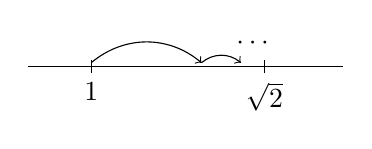
\begin{tikzpicture}
  \draw (0,0) -- (4,0);
  \draw (0.8,0.08) -- (0.8,-0.08) node[below] {$1$};
  \draw (3,0.08) -- (3,-0.08) node[below] {$\sqrt2$};
  \draw[->] (0.8,0.05) to[out=40,in=140] (2.2,0.05);
  \draw[->] (2.2,0.05) to[out=40,in=140] (2.7,0.05);
  \node at (2.85,0.3) {$\cdots$};
\end{tikzpicture}
\end{center}
Since $\sqrt2\notin\V$: $\therefore$ \key{$\{v_n\}$ is not convergent (in $\V$).}

\paragraph{What about Cauchyness?}
\[
\norm{v_n - v_m} \to 0 \text{ as } n,m\to\infty
\]
$v_n$ is actually Cauchy as elements are approaching each other.
\explain{Indeed $v_n$ and $v_m$ agree in the first $\min(n,m)$ decimals, so $|v_n - v_m| < 10^{-\min(n,m)} \to 0$.}
\[
\therefore\ \text{\key{Convergent $\Rightarrow$ Cauchy}} \quad\text{but}\quad \text{Cauchy} \not\Rightarrow \text{Convergent}
\]
\explain{Margin note (Turkish): ``ben bi sequence olsam sana converge ederdim.''}
\end{example}
If a set does not have holes $\Rightarrow$ \key{complete} set.
\begin{insight}
The same sequence viewed in $\V=\R$ converges (to $\sqrt2\in\R$): convergence depends on the space, not only on the terms. $\R$ is complete (it ``fills the holes'' of $\Q$), and so is every finite-dimensional normed space over $\R$ or $\C$, e.g.\ $(\R^n,\norm{\cdot}_p)$. Incompleteness is therefore a phenomenon of infinite-dimensional spaces such as function spaces, as the next example shows.
\end{insight}

\begin{definition}
A normed space is said to be \term{complete} iff \key{every Cauchy sequence is convergent}. A complete normed space is called a \term{Banach space}.
\end{definition}
\begin{example}
A normed space defined as
\[
\V = \left\{ f(\cdot) \;\middle|\; f:[-1,1]\to\R,\ f \text{ is continuous } \& \int_{-1}^{1}|f(t)|\,dt < \infty\right\},
\qquad
\norm{f}_1 = \int_{-1}^{1}|f(t)|\,dt
\]
Consider the sequence $\{f_n\}_{n=1}^\infty$:
\[
f_n(t) = \begin{cases} 1, & -1\le t\le 0\\ 1 - nt, & 0\le t\le \frac1n\\ 0, & \frac1n\le t\le 1\end{cases}
\]
\begin{center}
\pgfplotsset{fnplot/.style={width=4.6cm,height=3.4cm,axis lines=middle,
  xmin=-1.3,xmax=1.35,ymin=-0.15,ymax=1.35,ytick={1},
  yticklabel style={anchor=south west,font=\small},
  every axis y label/.style={at={(current axis.above origin)},anchor=south west}}}
\begin{tikzpicture}
\begin{axis}[fnplot,name=a1,xtick={-1,1},ylabel={$f_1(t)$},xlabel={$t$},
  every axis x label/.style={at={(current axis.right of origin)},anchor=west}]
  \addplot[thick] coordinates {(-1,0) (-1,1) (0,1) (1,0)};
\end{axis}
\begin{axis}[fnplot,name=a2,at={(a1.east)},anchor=west,xshift=0.6cm,
  xtick={-1,0.5,1},xticklabels={$-1$,$\frac12$,$1$},ylabel={$f_2(t)$}]
  \addplot[thick] coordinates {(-1,0) (-1,1) (0,1) (0.5,0) (1,0)};
\end{axis}
\node at ($(a2.east)+(0.35,0)$) {$\cdots$};
\begin{axis}[fnplot,name=a3,at={(a2.east)},anchor=west,xshift=0.7cm,
  xtick={-1,0.25,1},xticklabels={$-1$,$\frac1n$,$1$},ylabel={$f_n(t)$}]
  \addplot[thick] coordinates {(-1,0) (-1,1) (0,1) (0.25,0) (1,0)};
\end{axis}
\end{tikzpicture}
\end{center}
Is the sequence $\{f_n\}$ Cauchy? Convergent?
\[
\norm{f_n(t) - f_m(t)}_1 = \int_{-1}^{1}|f_n(t) - f_m(t)|\,dt
\]
\begin{center}
\begin{minipage}{0.45\textwidth}
\centering
\begin{tikzpicture}
\begin{axis}[width=5.4cm,height=3.8cm,axis lines=middle,
  xmin=-1.3,xmax=1.35,ymin=-0.15,ymax=1.3,ytick={1},yticklabel style={anchor=south west},
  xtick={-1,0.3,0.6,1},xticklabels={$-1$,$\frac1m$,$\frac1n$,$1$},clip=false]
  \addplot[pattern=north east lines,draw=none] coordinates {(0,1) (0.6,0) (0.3,0) (0,1)};
  \addplot[thick] coordinates {(-1,0) (-1,1) (0,1) (0.6,0) (1,0)};
  \addplot[thick] coordinates {(0,1) (0.3,0)};
  \draw (axis cs:0.33,0.45) -- (axis cs:0.75,0.95) node[right,font=\small,align=left] {difference\\integration\\is this area.};
\end{axis}
\end{tikzpicture}
\end{minipage}%
\begin{minipage}{0.5\textwidth}
\[
\text{Area} = \left|\frac1n - \frac1m\right|\cdot\frac12
\]
\explain{Triangle with vertices $(0,1)$, $(\frac1m,0)$, $(\frac1n,0)$: base $|\frac1n-\frac1m|$, height $1$.}
\[
\lim_{n,m\to\infty}\left|\frac1n - \frac1m\right|\cdot\frac12 = 0
\]
\end{minipage}
\end{center}
\begin{center}
\begin{minipage}{0.45\textwidth}
\centering
\begin{tikzpicture}
\begin{axis}[width=5.4cm,height=3.8cm,axis lines=middle,
  xmin=-1.3,xmax=1.35,ymin=-0.15,ymax=1.3,ytick={1},yticklabel style={anchor=south west},
  xtick={-1,0,1},title={$f_n \xrightarrow{\,n\to\infty\,}$},title style={font=\small}]
  \addplot[thick] coordinates {(-1,0) (-1,1) (0,1) (0,0) (1,0)};
\end{axis}
\end{tikzpicture}
\end{minipage}%
\begin{minipage}{0.5\textwidth}
The limit $\notin\V$ (not continuous).

$\Rightarrow \{f_n\}$ is Cauchy but not convergent.

$\therefore$ \key{$(\V,\F,\norm{\cdot}_1)$ is not complete.}
\end{minipage}
\end{center}
\begin{insight}
To be precise, ``not convergent'' means no \emph{continuous} $g$ satisfies $\norm{f_n - g}_1\to 0$. If one did, then on $[-1,0]$ we would need $\int_{-1}^0|1-g|\,dt = 0$, so $g = 1$ there; and on every $[\delta,1]$, $\delta>0$, $f_n = 0$ eventually, so $g = 0$ there. Then $g$ jumps at $t = 0$, contradicting continuity. The ``limit'' is the step function, which lies outside $\V$.
\end{insight}
\end{example}

% ===== Page 18 =====
\origpage{18}
\paragraph{Now with $(\V,\F,\norm{\cdot}_\infty)$.}
\begin{align*}
\norm{f}_\infty &= \max_{-1\le t\le 1}|f(t)|\\
\norm{f_n(t) - f_m(t)}_\infty &= \max_{-1\le t\le 1}|f_n(t) - f_m(t)|
\end{align*}
\begin{center}
\begin{minipage}{0.4\textwidth}
\begin{align*}
f_n(t) &= 1 - nt \quad \big(0\le t\le\tfrac1n\big)\\
f_n\!\left(\tfrac1m\right) &= 1 - \frac nm \quad (m\ge n)
\end{align*}
\end{minipage}%
\begin{minipage}{0.5\textwidth}
\centering
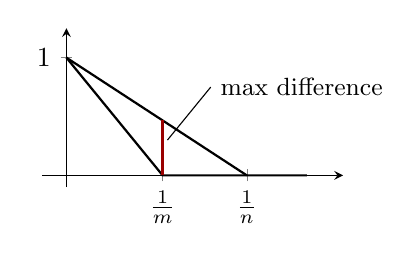
\begin{tikzpicture}
\begin{axis}[width=5.4cm,height=3.6cm,axis lines=middle,
  xmin=-0.1,xmax=1.15,ymin=-0.1,ymax=1.25,ytick={1},
  xtick={0.4,0.75},xticklabels={$\frac1m$,$\frac1n$},clip=false]
  \addplot[thick] coordinates {(0,1) (0.4,0) (1,0)};
  \addplot[thick] coordinates {(0,1) (0.75,0)};
  \addplot[very thick,red!60!black] coordinates {(0.4,0) (0.4,{1-0.4/0.75})};
  \draw (axis cs:0.42,0.3) -- (axis cs:0.6,0.75) node[right,font=\small] {max difference};
\end{axis}
\end{tikzpicture}
\end{minipage}
\end{center}
% corrected: notes wrote lim_{n,m} ||f_n - f_m||_inf = |1 - n/m|; the distance itself equals |1 - n/m| (m >= n), and this does not tend to 0
\begin{align*}
\norm{f_n(t) - f_m(t)}_\infty &= f_n\!\left(\tfrac1m\right) - \underbrace{f_m\!\left(\tfrac1m\right)}_{0} = {\underbrace{\left|1 - \frac nm\right|}_{\neq 0 \text{ unless } n=m}} \qquad (m\ge n)\\
\text{e.g.\ } m = 2n:\quad \norm{f_n - f_{2n}}_\infty &= \tfrac12 \quad \text{for every } n
\end{align*}
\begin{center}
\fbox{\begin{minipage}{0.75\textwidth}\small\itshape
$n$ ve $m$'in nasıl $\infty$'a gittiği fark etmez, her zaman limit sonucu sıfır olmalı. Bu senaryoda if $n=m$ o zaman limit sıfır, onun dışında değil.
\end{minipage}}
\end{center}
% translation: it does not matter how n and m go to infinity, the limit must always be zero.
% In this scenario the limit is zero only if n = m, not otherwise.
\explain{It does not matter how $n$ and $m$ go to $\infty$; the limit must always be zero. Here it is zero only if $n=m$.}
\explain{The maximum is at $t=\frac1m$: on $[0,\frac1m]$ the difference $(m-n)t$ increases, and on $[\frac1m,\frac1n]$ it equals $1-nt$, which decreases.}
$\therefore$ \key{$\{f_n\}$ is not Cauchy} in the sup norm.

% Section 3: Inner Product Spaces  (original handwritten pages 19--24)
\section{Inner Product Spaces}\label{sec:ips}
\syllabusweek{Week 4 --- inner product spaces, orthogonality, Gram--Schmidt}
\subsection{Inner Products}\label{ss:inner-products}
\begin{definition}
Let $(\V,\C)$ be a vector space. An \term{inner product} is a function from $\V\times\V$ into $\C$,
\[
\inner{\cdot}{\cdot} : \V\times\V\to\C
\]
satisfying the following properties:
\begin{enumerate}[label=\arabic*)]
\item $\inner{x}{y} = \overline{\inner{y}{x}}$ \quad $\forall x,y\in\V$ \hfill (conjugate symmetry)
\item Linearity with respect to (w.r.t.) the first argument:
  \begin{enumerate}[label=\alph*)]
  \item $\inner{x+y}{z} = \inner{x}{z} + \inner{y}{z}$ \quad $\forall x,y,z\in\V$ \hfill (additivity)
  \item $\inner{\alpha x}{y} = \alpha\inner{x}{y}$ \quad $\forall\alpha\in\C$ and $\forall x,y\in\V$ \hfill (homogeneity)
  \end{enumerate}
\item $\inner{x}{x}$ is real \& nonnegative, $\inner{x}{x}\ge 0$, and
  $\inner{x}{x} = 0 \Leftrightarrow x = 0_{\V}$ \hfill (positive definiteness)
\end{enumerate}
$\therefore$ The triplet $(\V,\C,\inner{\cdot}{\cdot})$ is called an \term{inner product space}.
\end{definition}
\begin{align*}
\inner{x}{y+z} &= \overline{\inner{y+z}{x}} = \overline{\inner{y}{x}} + \overline{\inner{z}{x}} = \inner{x}{y} + \inner{x}{z}
\end{align*}
\explain{Additivity w.r.t.\ second argument \checkmark}
\begin{align*}
\inner{x}{\alpha y} &= \overline{\inner{\alpha y}{x}} = \bar\alpha\,\overline{\inner{y}{x}} = \bar\alpha\inner{x}{y}
\end{align*}
\explain{Homogeneity w.r.t.\ second argument $\times$ ($\alpha$ should be real). We have \key{conjugate homogeneity w.r.t.\ second argument}.}
\begin{insight}
So an inner product is linear in the first argument and \emph{conjugate}-linear in the second:
$\inner{\textstyle\sum_i\alpha_i x_i}{\sum_j\beta_j y_j} = \sum_{i,j}\alpha_i\bar\beta_j\inner{x_i}{y_j}$.
Over $\F=\R$ the conjugates disappear and the inner product is bilinear and symmetric. Also $\inner{x}{0_\V} = \inner{0_\V}{x} = 0$ for all $x$ (take $\alpha = 0$ in homogeneity).
\end{insight}

% ===== Page 19 =====
\origpage{19}
\begin{example}
$\V = \C^n$, $\F = \C$, \quad
$x = [x_1\ x_2 \ldots x_n]\T$, \ $y = [y_1\ y_2 \ldots y_n]\T$, \quad $x_i, y_i\in\C$.
\[
\inner{x}{y} = \sum_{i=1}^n x_i\bar y_i = \bar y\T x = y\Hm x
\qquad \Big(\begin{bmatrix} \bar y_1 & \bar y_2 & \cdots\end{bmatrix}\bmat{x_1\\ x_2\\ \vdots}\Big)
% corrected: notes had the row vector [y_1 y_2 ...]; y^H = conj(y)^T has conjugated entries
\]
\paragraph{Check of the axioms.}
\begin{enumerate}[label=\arabic*)]
\item $\inner{x}{y} = \sum_{i=1}^n x_i\bar y_i = \bar y\T x = y\Hm x$
\[
\overline{\inner{y}{x}} = \overline{x\Hm y} = \overline{\bar x\T y} = \underbrace{x\T\bar y = \bar y\T x}_{\text{scalar} = \text{its transpose}} = y\Hm x = \inner{x}{y}
\]
\needspace{3\baselineskip}
\item \begin{enumerate}[label=\alph*)]
  \item $\inner{x+y}{z} = z\Hm(x+y) = z\Hm x + z\Hm y = \inner{x}{z} + \inner{y}{z}$
  \item $\inner{\alpha x}{y} = y\Hm(\alpha x) = \alpha y\Hm x = \alpha\inner{x}{y}$
  \end{enumerate}
\item $\inner{x}{x} = x\Hm x = \sum_{i=1}^n |x_i|^2 \ge 0 \;\Rightarrow$ real value;
  \ $\inner{x}{x} = 0 \Leftrightarrow x = 0_\V$.
\end{enumerate}
\end{example}
\begin{example}
$A, B\in\R^{m\times n}$, \ $\V=\R^{m\times n}$, \ $\F=\R$, \ $A = [a_{ij}]$, \ $B = [b_{ij}]$:
\[
\inner{A}{B} = \sum_{i,j} a_{ij}b_{ij}
\]
\[
\underbrace{\bmat{a_{11} & a_{12} & a_{13}\\ a_{21} & a_{22} & a_{23}}\cdot
\bmat{b_{11} & b_{21}\\ b_{12} & b_{22}\\ b_{13} & b_{23}}}_{A\cdot B\T}
=
\bmat{a_{11}b_{11} + a_{12}b_{12} + a_{13}b_{13} & \times\\ \times & a_{21}b_{21} + a_{22}b_{22} + a_{23}b_{23}}
\]
% corrected: notes had B^T with rows b11 b12 / b12 b22 / b13 b23 (entry (1,2) must be b21)
\begin{align*}
\inner{A}{B} &\triangleq \tr(AB\T)\\
&= \tr(A\T B) \quad \text{(in the real field)}
\end{align*}
\explain{$(AB\T)_{ii} = \sum_j a_{ij}b_{ij}$ (row $i$ of $A$ against row $i$ of $B$), so the trace adds up all $a_{ij}b_{ij}$; the off-diagonal entries ($\times$) are irrelevant. For complex matrices one uses $\inner{A}{B} = \tr(AB\Hm) = \tr(B\Hm A)$, whose induced norm is the Frobenius norm.}
\end{example}
\begin{example}
$\V = \left\{ f(\cdot) \;\middle|\; f:[0,1]\to\C \text{ s.t. } \int_0^1 |f(t)|^2\,dt < \infty\right\}$
\[
\inner{f_1}{f_2} \triangleq \int_0^1 f_1(t)\overline{f_2(t)}\,dt \qquad (\mathcal{L}_2 \text{ inner product})
\]
\end{example}
\subsection{The Cauchy--Schwarz Inequality and the Induced Norm}\label{ss:cauchy-schwarz}
\begin{theorem}[Cauchy--Schwarz Inequality]
Let $\V$ be an inner product space. Let $x,y\in\V$.
\[
|\inner{x}{y}|^2 \le \inner{x}{x}\inner{y}{y}
\]
Equality holds iff $x = cy$ for some $c\in\C$ or $y = 0_\V$, i.e.\ \key{equality iff $x$ and $y$ are linearly dependent}.
\end{theorem}
% corrected: notes stated equality iff x = cy; the case y = 0_V (x arbitrary) also gives equality 0 = 0, so the condition is linear dependence
\paragraph{Equality check for $x = cy$.}
\begin{align*}
\inner{x}{y} &= \inner{cy}{y} = c\inner{y}{y} \;\Rightarrow\; |\inner{x}{y}|^2 = |c|^2\inner{y}{y}^2\\
\inner{x}{x} &= \inner{cy}{cy} = c\bar c\inner{y}{y} = |c|^2\inner{y}{y} \qquad (c\bar c = |c|^2 \text{ is real})
\end{align*}
\explain{Using the first- and second-argument axioms.}
\[
\underbrace{|c|^2\inner{y}{y}^2}_{|\inner{x}{y}|^2} = \underbrace{|c|^2\inner{y}{y}}_{\inner{x}{x}}\underbrace{\inner{y}{y}}_{\inner{y}{y}}
\]

% ===== Page 20 =====
\origpage{20}
\needspace{6\baselineskip}
\begin{proof}[Proof of theorem]
We distinguish two cases.
\paragraph{Case 1: $y = 0_{\V}$.}
\begin{align*}
\inner{x}{y} &= \inner{x}{0_{\V}} = \inner{x}{0\cdot 0_{\V}} = 0\cdot\inner{x}{0_{\V}} = 0\\
\inner{y}{y} &= 0 \quad \text{(by axioms)}\\
\underbrace{|\inner{x}{y}|^2}_{0} &\le \underbrace{\inner{x}{x}}_{\ge 0}\underbrace{\inner{y}{y}}_{0} \;\Rightarrow\; 0\le 0 \ \checkmark
\end{align*}
\paragraph{Case 2: $y\neq 0_{\V}$.} Then $\inner{y}{y}\neq 0$ (in fact $\inner{y}{y}>0$ by axiom 3, so we may divide by it and multiply inequalities by it).
For $\alpha\in\C$ (in field):
\begin{align*}
0 &\le \inner{x-\alpha y}{x-\alpha y}\\
&= \inner{x}{x} - \inner{x}{\alpha y} - \inner{\alpha y}{x} + \inner{\alpha y}{\alpha y}\\
&= \inner{x}{x} - \bar\alpha\inner{x}{y} - \alpha{\underbrace{\inner{y}{x}}_{\overline{\inner{x}{y}}}} + |\alpha|^2\inner{y}{y}
\end{align*}
Choose $\displaystyle \alpha = \frac{\inner{x}{y}}{\inner{y}{y}}$:
\begin{align*}
0 &\le \inner{x}{x} - \frac{\overline{\inner{x}{y}}}{\inner{y}{y}}\cdot\inner{x}{y} - \cancel{\frac{\inner{x}{y}}{\inner{y}{y}}\cdot\overline{\inner{x}{y}}} + \cancel{\frac{|\inner{x}{y}|^2}{\inner{y}{y}^2}\cdot\inner{y}{y}}\\
0 &\le \inner{x}{x} - \frac{|\inner{x}{y}|^2}{\inner{y}{y}}\\
\frac{|\inner{x}{y}|^2}{\inner{y}{y}} &\le \inner{x}{x} \;\Rightarrow\; \therefore\ |\inner{x}{y}|^2 \le \inner{x}{x}\inner{y}{y}
\qedhere
\end{align*}
\end{proof}
\begin{insight}[Choice of $\alpha$ and the equality case]
$\alpha y$ with $\alpha = \inner{x}{y}/\inner{y}{y}$ is the projection of $x$ onto $y$ (see Gram--Schmidt below), so $x-\alpha y\perp y$ and the first line says $\norm{x-\alpha y}^2\ge 0$: the error of the best approximation of $x$ along $y$ has nonnegative length.
Equality in the theorem (with $y\neq 0_\V$) holds iff $\inner{x-\alpha y}{x-\alpha y} = 0$, i.e.\ iff $x = \alpha y$ by axiom 3. This proves the ``only if'' part of the equality statement; the ``if'' part is the check for $x = cy$ above.
\end{insight}

\begin{remark}
An inner product \key{induces a norm} (the \term{induced norm}) defined as
\[
\norm{x}^2 \triangleq \inner{x}{x}, \qquad \norm{x} \triangleq \sqrt{\inner{x}{x}}
\]
\end{remark}
\paragraph{Show that this is a norm.}
\begin{enumerate}[label=\arabic*)]
\item $\norm{x}\ge 0$, \ $\norm{x} = 0 \Leftrightarrow x = 0_{\V}$ \checkmark \ (by axiom 3 of the inner product) \hfill (positive definiteness)
\item $\displaystyle \norm{\alpha x} \triangleq \sqrt{\inner{\alpha x}{\alpha x}} = \sqrt{\alpha\cdot\bar\alpha\inner{x}{x}}
= |\alpha|\underbrace{\sqrt{\inner{x}{x}}}_{\norm{x}} = |\alpha|\norm{x}$ \checkmark \hfill (absolute homogeneity)
\item $\norm{x+y} = \sqrt{\inner{x+y}{x+y}}$ \hfill (triangle inequality)
\begin{align*}
\norm{x+y}^2 &= \inner{x+y}{x+y} = \inner{x}{x} + \inner{x}{y} + {\underbrace{\inner{y}{x}}_{\overline{\inner{x}{y}}}} + \inner{y}{y}\\
&= \inner{x}{x} + 2\cdot\operatorname{Re}\inner{x}{y} + \inner{y}{y}\\
&\le \inner{x}{x} + 2|\operatorname{Re}\inner{x}{y}| + \inner{y}{y}\\
&\le \inner{x}{x} + 2|\inner{x}{y}| + \inner{y}{y}
\intertext{\origpage{21}By Cauchy--Schwarz, $|\inner{x}{y}| \le \sqrt{\inner{x}{x}\inner{y}{y}}$:}
% ===== Page 21 =====
&\le \inner{x}{x} + 2\sqrt{\inner{x}{x}}\sqrt{\inner{y}{y}} + \inner{y}{y}\\*
&= \left(\sqrt{\inner{x}{x}} + \sqrt{\inner{y}{y}}\right)^2\\*
&= (\norm{x} + \norm{y})^2\\*
\norm{x+y}^2 &\le (\norm{x} + \norm{y})^2 \;\Rightarrow\; \norm{x+y}\le\norm{x}+\norm{y} \ \checkmark
\end{align*}
\explain{Both sides are nonnegative, so taking square roots preserves the inequality: the triangle inequality holds.}
\end{enumerate}

\sep
\paragraph{Angle between vectors.} By Cauchy--Schwarz, $|\inner{x}{y}| \le \norm{x}\norm{y}$; \ suppose $x\neq 0_{\V}$, $y\neq 0_{\V}$:
\[
0 \le \frac{|\inner{x}{y}|}{\norm{x}\norm{y}} \le 1
\]
\[
\cos\theta \triangleq \frac{|\inner{x}{y}|}{\norm{x}\norm{y}} \;\Rightarrow\; \theta = \arccos\left(\frac{|\inner{x}{y}|}{\norm{x}\norm{y}}\right)
\]
\explain{Cauchy--Schwarz is exactly what makes this angle well defined. With the absolute value $\theta\in[0,\frac\pi2]$; in a real space one often drops it, $\cos\theta = \frac{\inner{x}{y}}{\norm{x}\norm{y}}\in[-1,1]$, which for $\R^2,\R^3$ is the usual geometric angle. $\theta = \frac\pi2$ $\Leftrightarrow$ $\inner{x}{y}=0$ (orthogonal), $\theta = 0$ $\Leftrightarrow$ $x = cy$.}
\begin{remark}
\key{Every inner product space is also a normed space.} The converse/reverse is not correct in general.
\end{remark}
\begin{insight}
A norm comes from an inner product \key{iff it satisfies the parallelogram law}
$\norm{x+y}^2 + \norm{x-y}^2 = 2\norm{x}^2 + 2\norm{y}^2$.
For example $\norm{\cdot}_1$ on $\R^2$ fails it: $x = e_1$, $y = e_2$ give $4+4 = 8 \neq 4 = 2+2$. So $\ell_1$ and $\ell_\infty$ are norms without an inner product behind them; only $\ell_2$ is induced by $\inner{x}{y} = y\T x$.
\end{insight}
\begin{definition}
An inner product space that is complete w.r.t.\ the induced norm is called a \term{complete inner product space} / \term{Hilbert space}.
\end{definition}
\subsection{Orthogonality and Orthogonal Expansions}\label{ss:orthogonality}
\begin{definition}
Two vectors $x,y\in\V$ are said to be \term{orthogonal} iff $\inner{x}{y} = 0$.
Similarly subsets $S_1, S_2\subset\V$ are orthogonal iff $\inner{x}{y} = 0$ $\forall x\in S_1$, $\forall y\in S_2$.
\end{definition}
\needspace{9\baselineskip}
\paragraph{Examples.}
\begin{enumerate}[label=\arabic*)]
\item $\V=\R^n$, $\F=\R$, \quad $\inner{x}{y} = \sum_{i=1}^n x_iy_i = y\T x = x\T y$
\[
\underbrace{B = \{e_1, e_2, \ldots, e_n\}}_{\text{canonical basis set}} \qquad
e_1 = \bmat{1\\ 0\\ \vdots\\ 0} \quad e_2 = \bmat{0\\ 1\\ 0\\ \vdots\\ 0} \quad \cdots
\]
\[
\inner{e_i}{e_j} = \begin{cases} 0, & i\neq j\\ 1, & i = j\end{cases} = \delta_{ij}
\]
\item $\V = \left\{ f(\cdot) \;\middle|\; f:[-\pi,\pi]\to\C \text{ s.t. } \int_{-\pi}^{\pi}|f(t)|^2\,dt < \infty\right\}$

Consider $\{e^{jnt}\}_{n=-\infty}^{\infty}$, \quad $e^{jnt}\in\V$ for all $n$.
\[
\inner{f_1(t)}{f_2(t)} = \int_{-\pi}^{\pi} f_1(t)\,\overline{f_2(t)}\,dt
\]
\begin{align*}
\inner{e^{jnt}}{e^{jmt}} &= \int_{-\pi}^{\pi} e^{jnt}\,e^{-jmt}\,dt = \int_{-\pi}^{\pi} e^{j(n-m)t}\,dt\\
&= \int_{-\pi}^{\pi}\big[\cos((n-m)t) + j\sin((n-m)t)\big]\,dt\\
% ===== Page 22 =====
&= \int_{-\pi}^{\pi}\cos((n-m)t)\,dt + j\underbrace{\cancel{\int_{-\pi}^{\pi}\sin((n-m)t)\,dt}}_{0}
\end{align*}
\origpage{22}
\begin{center}
\begin{minipage}{0.5\textwidth}
\small $\left.\begin{array}{l}\sin t\\ \sin 2t\\ \sin 3t\\ \ \vdots\end{array}\right\}$ all zero due to integral over a period
\end{minipage}%
\begin{minipage}{0.35\textwidth}
\centering
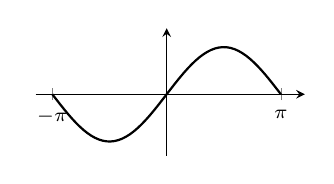
\begin{tikzpicture}
\begin{axis}[width=5cm,height=3.2cm,axis lines=middle,
  xmin=-3.6,xmax=3.8,ymin=-1.3,ymax=1.4,xtick={-3.1416,3.1416},xticklabels={$-\pi$,$\pi$},
  ytick=\empty,tick label style={font=\scriptsize}]
  \addplot[thick,domain=-pi:pi,samples=60] {sin(deg(x))};
\end{axis}
\end{tikzpicture}
\end{minipage}
\end{center}
\begin{align*}
\inner{e^{jnt}}{e^{jmt}} &= \begin{cases} 2\pi, & n = m\\ 0, & n\neq m\end{cases}\\
&= 2\pi\,\delta_{nm}
\end{align*}
\explain{For $n=m$: $\int_{-\pi}^{\pi}\cos 0\,dt = 2\pi$. For $k = n-m\neq0$: $\int_{-\pi}^{\pi}\cos kt\,dt = \frac{2\sin k\pi}{k} = 0$, and $\int_{-\pi}^{\pi}\sin kt\,dt = 0$ since $\sin kt$ is odd.}
\item $S_1 = \{\sin nt\}_{n=1}^\infty$, \ $S_2 = \{\cos mt\}_{m=1}^\infty$:
\begin{align*}
\inner{\sin nt}{\cos mt} &= \int_{-\pi}^{\pi}\sin nt\cdot\cos mt\,dt\\
&= \int_{-\pi}^{\pi}\frac12\Big(\underbrace{\cancel{\sin((n+m)t)}}_{0} + \underbrace{\cancel{\sin((n-m)t)}}_{0}\Big)\,dt = 0
\end{align*}
\explain{Product-to-sum: $\sin a\cos b = \frac12[\sin(a+b)+\sin(a-b)]$; both terms are odd functions (or zero when $n=m$), so they integrate to $0$ over the symmetric interval $[-\pi,\pi]$.}
\[
\therefore\ \key{$S_1\perp S_2$}
\]
\end{enumerate}

\sep
\paragraph{Expansion in an orthogonal set.}
\begin{itemize}
\item $z = \alpha_1 z_1 + \alpha_2 z_2$ \quad if $z_1\perp z_2$:
\begin{align*}
\inner{z}{z_1} &= \inner{\alpha_1 z_1 + \alpha_2 z_2}{z_1}\\
&= \alpha_1\inner{z_1}{z_1} + \alpha_2\underbrace{\cancel{\inner{z_2}{z_1}}}_{0} \;\Rightarrow\; \alpha_1 = \frac{\inner{z}{z_1}}{\inner{z_1}{z_1}}
\end{align*}
In general,
\[
z = \sum_{i=1}^n \alpha_i z_i, \qquad \alpha_i = \frac{\inner{z}{z_i}}{\inner{z_i}{z_i}} \quad \forall i
\]
\explain{Valid when $z\in\Span\{z_1,\ldots,z_n\}$ and the $z_i\neq 0_\V$ are mutually orthogonal: take $\inner{\cdot}{z_k}$ of both sides and all terms with $i\neq k$ vanish. \key{No linear system has to be solved; each coefficient is computed independently.}}
\paragraph{Example (as $z_1\perp z_2$).}
\[
{\underbrace{\bmat{2\\ 3}}_{z}} = \beta_1{\underbrace{\bmat{1\\ 1}}_{z_1}} + \beta_2{\underbrace{\bmat{1\\ -1}}_{z_2}},
\qquad
\beta_1 = \frac{\inner{z}{z_1}}{\inner{z_1}{z_1}} = \frac{5}{2},
\qquad
\beta_2 = \frac{\inner{z}{z_2}}{\inner{z_2}{z_2}} = \frac{2-3}{2} = -\frac12
\]
\explain{Check: $\frac52\bmat{1\\1} - \frac12\bmat{1\\-1} = \bmat{2\\3}$ \checkmark}
\item $f(t) = \sum_{n=-\infty}^{\infty}\alpha_n e^{jnt}$:
\[
\alpha_n = \frac{\inner{f(t)}{e^{jnt}}}{\inner{e^{jnt}}{e^{jnt}}} = \frac{1}{2\pi}\int_{-\pi}^{\pi} f(t)e^{-jnt}\,dt \qquad \text{(Fourier series coefficients)}
\]
\explain{With $\inner{f_1}{f_2} = \int_{-\pi}^{\pi} f_1(t)\,\overline{f_2(t)}\,dt$.}
\end{itemize}

% ===== Page 23 =====
\subsection{Gram--Schmidt Orthogonalization}\label{ss:gram-schmidt}
\origpage{23}%
\paragraph{Question.} Let $\V$ be an inner product space. Let $S_1 = \{v_1, v_2, \ldots, v_n\}$ be a linearly independent set. Can we obtain another set $S_2 = \{w_1, w_2, \ldots, w_n\}$ such that
\begin{enumerate}[label=\arabic*)]
\item $w_i\perp w_j$ when $i\neq j$
\item $\Span\{S_1\} = \Span\{S_2\}$?
\end{enumerate}
\key{Yes!} (constructively, by the following algorithm)

\needspace{9\baselineskip}
\paragraph{Gram--Schmidt orthogonalization algorithm.} The $w_k$ are constructed one at a time.
\paragraph{Step 1.} $w_1 = v_1$

\paragraph{Step 2.} $\displaystyle w_2 = v_2 - \frac{\inner{v_2}{w_1}}{\inner{w_1}{w_1}}\cdot w_1$
\begin{align*}
\inner{w_2}{w_1} &= \inner{v_2 - \frac{\inner{v_2}{w_1}}{\inner{w_1}{w_1}}\cdot w_1}{w_1}\\
&= \cancel{\inner{v_2}{w_1}} - \underbrace{\frac{\cancel{\inner{v_2}{w_1}}}{\cancel{\inner{w_1}{w_1}}}}_{\text{scalar}}\cancel{\inner{w_1}{w_1}} = 0
\end{align*}
\begin{center}
\begin{minipage}{0.55\textwidth}
\centering
\begin{tikzpicture}[scale=1.5]
  \coordinate (O) at (0,0);
  \coordinate (V1) at (1,2.4);
  \coordinate (V2) at (2.6,0.7);
  % projection of v2 onto v1: k = <v2,v1>/<v1,v1>
  \pgfmathsetmacro{\k}{(1*2.6+2.4*0.7)/(1*1+2.4*2.4)}
  \coordinate (P) at ({\k*1},{\k*2.4});
  \draw[->,thick,blue!60!black] (O) -- (V1) node[above] {$v_1 = w_1$};
  \draw[->,thick] (O) -- (V2) node[right] {$v_2$};
  \draw[->,very thick,red!60!black] (O) -- (P);
  \draw[->,very thick,red!80!black] (O) -- ($(O)!0.42!(P)$);
  \node[red!60!black,left,font=\small] at ($(O)!0.25!(P)+(-0.05,0)$) {$\frac{w_1}{\norm{w_1}}$};
  \draw[->,thick] (P) -- (V2) node[midway,above right] {$w_2$};
  \draw[dashed,red!60!black] (P) -- (V2);
  % right-angle mark at P
  \draw ($(P)!0.12cm!(V2)$) -- ($(P)!0.12cm!(V2)+(P)!0.12cm!(V1)-(P)$) -- ($(P)!0.12cm!(V1)$);
  \node[red!60!black,left,font=\small] at ($(P)+(-0.45,0.25)$) {$\frac{\inner{v_2}{w_1}}{\inner{w_1}{w_1}}\cdot w_1$};
  \draw[->,red!60!black] ($(P)+(-0.5,0.2)$) -- ($(P)+(-0.05,0.02)$);
  \pic[draw,"$\theta$",angle radius=0.45cm,angle eccentricity=1.45] {angle = V2--O--V1};
\end{tikzpicture}
\end{minipage}%
\begin{minipage}{0.4\textwidth}
\[
\inner{x}{y} = \norm{x}\norm{y}\cos\theta
\]
\end{minipage}
\end{center}
\[
\frac{\inner{v_2}{w_1}}{\underbrace{\inner{w_1}{w_1}}_{\norm{w_1}^2}}\cdot w_1
= \frac{\inner{v_2}{w_1}}{\norm{w_1}}\cdot\frac{w_1}{\norm{w_1}}
= \underbrace{\inner{v_2}{\frac{w_1}{\norm{w_1}}}}_{\norm{v_2}\cos\theta}\frac{w_1}{\norm{w_1}}
\]

\paragraph{Step 3.} $\displaystyle w_3 = v_3 - \frac{\inner{v_3}{w_1}}{\inner{w_1}{w_1}}\cdot w_1 - \frac{\inner{v_3}{w_2}}{\inner{w_2}{w_2}}\cdot w_2$
\[
\frac{\inner{v_i}{w_j}}{\inner{w_j}{w_j}}\cdot w_j \;:\; \text{\term{projection} of } v_i \text{ onto } w_j
\]

\paragraph{Step $n$.} $\displaystyle w_n = v_n - \sum_{i=1}^{n-1}\frac{\inner{v_n}{w_i}}{\inner{w_i}{w_i}}\cdot w_i$
\begin{insight}[Why Gram--Schmidt works]
\emph{Orthogonality} (by induction): if $w_1,\ldots,w_{k-1}$ are mutually orthogonal, then for $j<k$
$\inner{w_k}{w_j} = \inner{v_k}{w_j} - \sum_{i<k}\frac{\inner{v_k}{w_i}}{\inner{w_i}{w_i}}\inner{w_i}{w_j} = \inner{v_k}{w_j} - \inner{v_k}{w_j} = 0$,
since only the $i=j$ term survives.
\emph{Same span}: each $w_k$ is $v_k$ minus a combination of $w_1,\ldots,w_{k-1}\in\Span\{v_1,\ldots,v_{k-1}\}$, so $\Span\{w_1,\ldots,w_k\} = \Span\{v_1,\ldots,v_k\}$ for every $k$.
\emph{No division by zero}: $w_k = 0_\V$ would make $v_k\in\Span\{v_1,\ldots,v_{k-1}\}$, impossible for a linearly independent $S_1$; so $\inner{w_k}{w_k}>0$.
In words: \key{$w_k$ is the component of $v_k$ orthogonal to the span of the previous vectors.}
\end{insight}

\begin{example}
$\V = \left\{ f \;\middle|\; f:[-1,1]\to\R,\ \int_{-1}^{1}(f(t))^2\,dt < \infty\right\}$, \quad $\F = \R$,
\[
\inner{f}{g} = \int_{-1}^{1} f(t)g(t)\,dt
\]
\[
S_1 = \{v_1, v_2, v_3\}, \qquad v_1(t) = 1, \quad v_2(t) = t, \quad v_3(t) = t^2,
\qquad\text{i.e.}\quad S_1 = \{1, t, t^2\}
\]

% ===== Page 24 =====
\origpage{24}
\begin{align*}
w_1 &= v_1 = 1\\
w_2 &= t - \frac{\overset{0}{\cancel{\inner{t}{1}}}}{\inner{1}{1}}\cdot 1 = t, \qquad \inner{t}{1} = \int_{-1}^{1} t\,dt = 0\\
w_3 &= t^2 - \frac{\inner{t^2}{1}}{\inner{1}{1}}\cdot 1 - \frac{\overset{0}{\cancel{\inner{t^2}{t}}}}{\inner{t}{t}}\cdot t = t^2 - \frac{2/3}{2} = t^2 - \frac13
\end{align*}
using
\begin{align*}
\inner{t^2}{1} &= \int_{-1}^{1} t^2\,dt = 2\int_0^1 t^2\,dt = \frac23\\
\inner{1}{1} &= \int_{-1}^{1} 1\,dt = 2\\
\inner{t^2}{t} &= \int_{-1}^{1} t^3\,dt = 0\\
\inner{t}{t} &= \int_{-1}^{1} t^2\,dt = \frac23
\end{align*}
\begin{center}
\begin{minipage}{0.45\textwidth}
\[
S_2 = \left\{1,\ t,\ t^2 - \tfrac13\right\}
\]
\centering \term{Legendre polynomials}
\end{minipage}%
\begin{minipage}{0.5\textwidth}
\centering
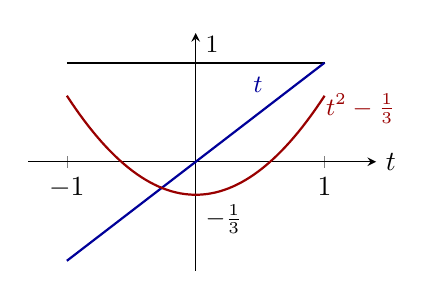
\begin{tikzpicture}
\begin{axis}[width=6cm,height=4.6cm,axis lines=middle,
  xmin=-1.3,xmax=1.4,ymin=-1.1,ymax=1.3,xtick={-1,1},ytick=\empty,xlabel={$t$},
  every axis x label/.style={at={(current axis.right of origin)},anchor=west},clip=false]
  \addplot[thick,domain=-1:1] {1};
  \node[above right,font=\small] at (axis cs:0,1) {$1$};
  \node[below right,font=\small] at (axis cs:0,-0.3333) {$-\frac13$};
  \addplot[thick,domain=-1:1,blue!60!black] {x} node[pos=0.8,above left,font=\small] {$t$};
  \addplot[thick,domain=-1:1,samples=60,red!60!black] {x^2-1/3} node[pos=0.95,right,font=\small] {$t^2-\frac13$};
\end{axis}
\end{tikzpicture}
\end{minipage}
\end{center}
\explain{Check: $\inner{t^2-\frac13}{1} = \frac23 - \frac13\cdot 2 = 0$ and $\inner{t^2-\frac13}{t} = \int_{-1}^1 (t^3 - \frac t3)\,dt = 0$ (odd integrand) \checkmark. These are the Legendre polynomials up to scaling: the standard ones are $P_0 = 1$, $P_1 = t$, $P_2 = \frac12(3t^2-1) = \frac32\big(t^2-\frac13\big)$, normalised so that $P_k(1) = 1$.}
\end{example}

\needspace{9\baselineskip}
\sep
\paragraph{Linearly dependent vectors.} If the vectors are linearly dependent, e.g.\ $S_1 = \{v_1, v_1\}$:
\begin{align*}
w_1 &= v_1\\
w_2 &= v_1 - \frac{\overset{1}{\cancel{\inner{v_1}{v_1}}}}{\cancel{\inner{v_1}{v_1}}}\cdot v_1 = 0
\end{align*}
\explain{When this is the case, \key{remove the redundant vector and resume the process}. In general $w_k = 0_\V$ exactly when $v_k$ depends linearly on $v_1,\ldots,v_{k-1}$; discarding such vectors, Gram--Schmidt returns an orthogonal basis of $\Span\{S_1\}$ (and its size is $\dim\Span\{S_1\}$).}

\needspace{12\baselineskip}
\paragraph{Gram--Schmidt orthonormalization.}
Require $\norm{w_i} = 1$, i.e.\ $\inner{w_i}{w_i} = 1$:
\begin{alignat*}{2}
\bar w_1 &= v_1, &\qquad w_1 &= \frac{\bar w_1}{\norm{\bar w_1}}\\*
\bar w_2 &= v_2 - \inner{v_2}{w_1}w_1, &\qquad w_2 &= \frac{\bar w_2}{\norm{\bar w_2}}\\*
&\ \,\vdots\\*
\bar w_n &= v_n - \sum_{i=1}^{n-1}\inner{v_n}{w_i}w_i, &\qquad w_n &= \frac{\bar w_n}{\norm{\bar w_n}}
\end{alignat*}
% corrected: notes had w_2 = \bar w_2 / ||w_2||; the normalisation divides by ||\bar w_2||. The last normalisation w_n = \bar w_n/||\bar w_n|| is implied by the pattern and added.
\explain{Since $\inner{w_i}{w_i} = 1$, the projection coefficients $\frac{\inner{v_k}{w_i}}{\inner{w_i}{w_i}}$ simplify to $\inner{v_k}{w_i}$. The resulting set is \term{orthonormal}: $\inner{w_i}{w_j} = \delta_{ij}$.}

% Section 4: Linear Transformations  (original handwritten pages 25--32)
\section{Linear Transformations}\label{sec:lt}
\syllabusweek{Week 5 --- linear transformations, null space, range space, matrix representations}
\subsection{Definition and Examples}\label{ss:lt-def}
\begin{definition}
Let $\V$ \& $\W$ be two vector spaces over the same field $\F$. A \term{linear transformation} $\mathcal{A}$ is a mapping from $\V$ into $\W$ shown as $\mathcal{A}:\V\to\W$ such that
\[
\mathcal{A}(\alpha_1 v_1 + \alpha_2 v_2) = \alpha_1\mathcal{A}v_1 + \alpha_2\mathcal{A}v_2
\]
for all $v_1,v_2\in\V$ and all $\alpha_1,\alpha_2\in\F$.
\end{definition}
\begin{center}
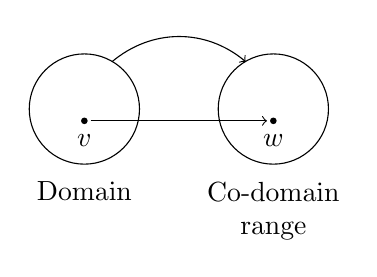
\begin{tikzpicture}
  \draw (0,0) circle (0.7);
  \draw (2.4,0) circle (0.7);
  \node at (0,0.35) {$\V$};
  \node at (2.4,0.35) {$\W$};
  \fill (0,-0.15) circle (1.2pt); \node at (0,-0.4) {$v$};
  \fill (2.4,-0.15) circle (1.2pt); \node at (2.4,-0.4) {$w$};
  \draw[->] (0.08,-0.15) -- (2.32,-0.15);
  \draw[->] (0.35,0.6) to[out=40,in=140] (2.05,0.6);
  \node[below] at (0,-0.8) {Domain};
  \node[below,align=center] at (2.4,-0.8) {Co-domain\\ range};
\end{tikzpicture}
\end{center}
\explain{$\V$ is the \term{domain} and $\W$ the \term{co-domain}; the \term{range} $\Range(\mathcal A) = \{\mathcal A v : v\in\V\}$ is the subset of $\W$ actually reached (in general $\Range(\mathcal A)\subseteq\W$).}
\begin{insight}
The single condition is equivalent to additivity $\mathcal A(v_1+v_2) = \mathcal Av_1+\mathcal Av_2$ together with homogeneity $\mathcal A(\alpha v) = \alpha\mathcal Av$. Taking $\alpha_1=\alpha_2=0$ gives $\mathcal A 0_\V = 0_\W$. Standard examples: $x\mapsto Ax$ for $A\in\F^{m\times n}$ ($\V=\F^n$, $\W=\F^m$, as in the induced-norm section), differentiation $f\mapsto f'$ on polynomials, and $f\mapsto\int_0^1 f(t)\,dt$.
\end{insight}

% ===== Page 25 =====
\needspace{8\baselineskip}
\begin{example}\leavevmode\origpage{25}
$\V=\W \triangleq \{\text{polynomials with degree} \le n\}$, \quad $\mathcal{A} = \dfrac{d}{dt}$,
\[
v_1=\sum_{i=0}^{n}\alpha_i t^i, \qquad v_2=\sum_{i=0}^{n}\beta_i t^i .
\]
% corrected: notes had the sums for v_1, v_2 starting at i=1 (constant term must be included; the next line already uses i=0)
\begin{align*}
a_1v_1+a_2v_2 &= \sum_{i=0}^{n}(a_1\alpha_i+a_2\beta_i)\,t^i\\
\mathcal{A}(a_1v_1+a_2v_2) &= \sum_{i=1}^{n}(a_1\alpha_i+a_2\beta_i)\cdot i\, t^{i-1}\\
&= a_1\sum_{i=1}^{n} i\alpha_i t^{i-1} + a_2\sum_{i=1}^{n} i\beta_i t^{i-1}\\
&= a_1\mathcal{A}v_1+a_2\mathcal{A}v_2
\end{align*}
\explain{The constant terms ($i=0$) differentiate to zero, which is why the sums after differentiation start at $i=1$. Hence $\frac{d}{dt}$ is linear.}
\end{example}

\begin{example}
$\V=\W=\R^2$, \quad $x=\bmat{\alpha_1\\ \alpha_2}$, \quad $y=\bmat{\beta_1\\ \beta_2}$.
\begin{align*}
\mathcal{A}x &= \bmat{\alpha_1\\ \alpha_1+\alpha_2}, \qquad
ax+by=\bmat{a\alpha_1+b\beta_1\\ a\alpha_2+b\beta_2}\\
\mathcal{A}(ax+by) &= \bmat{a\alpha_1+b\beta_1\\ a\alpha_1+b\beta_1+a\alpha_2+b\beta_2}\\
&= a\bmat{\alpha_1\\ \alpha_1+\alpha_2}+b\bmat{\beta_1\\ \beta_1+\beta_2} = a\mathcal{A}x+b\mathcal{A}y \ \checkmark
\end{align*}
\end{example}

\begin{example}
$\V=\W=\R$, \quad $\mathcal{A}x=1-x$.

\begin{center}
\begin{tikzpicture}
\begin{axis}[width=5.5cm, height=4.6cm, axis lines=middle, xmin=-1.3, xmax=2.6, ymin=-1.6, ymax=1.9,
  xtick={1}, ytick={1}, xlabel={$x$}, ylabel={$\mathcal{A}x$},
  xlabel style={anchor=west}, ylabel style={anchor=south}, tick label style={font=\scriptsize}]
\addplot[thick, domain=-0.8:2.5] {1-x};
\end{axis}
\end{tikzpicture}
\end{center}

Take $x_1=0$, $x_2=3$, $\alpha_1=1$, $\alpha_2=1$:
\begin{align*}
\alpha_1x_1+\alpha_2x_2 &= 1\cdot 0+1\cdot 3=3\\
\mathcal{A}(\alpha_1x_1+\alpha_2x_2) &= \mathcal{A}3=1-3=-2\\
\mathcal{A}x_1 &= 1, \qquad \mathcal{A}x_2=-2\\
\alpha_1\mathcal{A}x_1+\alpha_2\mathcal{A}x_2 &= -1
\end{align*}
\explain{$-2\ne-1$ $\Rightarrow$ \key{not a linear transformation.}}

\sep
The graph should pass through zero: \key{every linear transformation must satisfy $\mathcal{A}0_V=0_W$.}
\begin{align*}
\mathcal{A}(\alpha_1x_1+\cancel{\alpha_2x_2}^{\,0}) &= \alpha_1\mathcal{A}x_1+\cancel{\alpha_2\mathcal{A}x_2}^{\,0}
  && \text{(suppose } \alpha_2=0)\\
\mathcal{A}(\alpha_1x_1) &= \alpha_1\mathcal{A}(x_1) && \text{(suppose } \alpha_1=0)\\
\mathcal{A}(0_V) &= 0_W
\end{align*}
\begin{insight}[Quick test for linearity]
Every linear transformation maps $0_V$ to $0_W$ (take $\alpha_1=0$ in $\mathcal{A}(\alpha_1x_1)=\alpha_1\mathcal{A}x_1$). Here $\mathcal{A}0=1-0=1\ne0$, so $\mathcal{A}x=1-x$ cannot be linear: the graph is a straight line, but it does not pass through the origin (an \term{affine} map). The converse is false: $\mathcal{A}0=0$ alone does not guarantee linearity (e.g.\ $\mathcal{A}x=x^2$).
\end{insight}
\end{example}

% ===== Page 26 =====
\begin{example}\leavevmode\origpage{26}
\begin{align*}
\V &= \{f \mid f:[0,1]\to\R,\ f \text{ is integrable}\}, \qquad \W = \R\\
\mathcal{A}f &= \int_0^1 f(t)\,dt
\end{align*}
\explain{$\checkmark$ A linear transformation: $\int_0^1(af+bg)\,dt=a\int_0^1f\,dt+b\int_0^1g\,dt$ by linearity of the integral.}
\end{example}

\subsection{Null Space}\label{ss:null}

\begin{definition}
Let $\mathcal{A}:\V\to\W$ be a linear transformation. The \term{null space} of $\mathcal{A}$ is defined as
\[
\Null(\mathcal{A}) \triangleq \{v\in\V \mid \mathcal{A}v=0_W\}.
\]
\end{definition}

\begin{center}
\begin{minipage}{0.42\textwidth}\centering
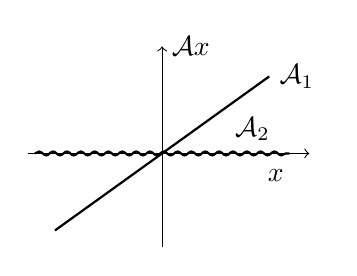
\begin{tikzpicture}[scale=0.85]
\draw[->] (-2,0) -- (2.2,0) node[right] {$\V$};
\node[below] at (1.7,-0.1) {$x$};
\draw[->] (0,-1.4) -- (0,1.6) node[right] {$\mathcal{A}x$};
\node[left] at (-0.1,1.5) {$\W$};
\draw[thick] (-1.6,-1.15) -- (1.6,1.15) node[right] {$\mathcal{A}_1$};
\draw[thick,decorate,decoration={snake,amplitude=0.7pt,segment length=5pt}] (-1.9,0) -- (1.9,0);
\node[above] at (1.35,0.05) {$\mathcal{A}_2$};
\end{tikzpicture}
\end{minipage}%
\begin{minipage}{0.4\textwidth}
\begin{align*}
\Null(\mathcal{A}_1)&=\{0_V\}\\
\Null(\mathcal{A}_2)&=\V=\R
\end{align*}
\end{minipage}
\end{center}
% corrected: notes had N(A_1) = 0_V (null space is a set: {0_V})
\explain{$\mathcal{A}_1$: a line through the origin with nonzero slope (only $x=0$ maps to $0$); $\mathcal{A}_2$: the zero map (every $x$ maps to $0$).}

\begin{claim}
\key{$\Null(\mathcal{A})$ is a subspace of $\V$.}
\end{claim}

\begin{center}
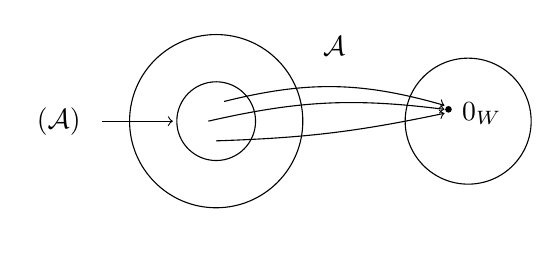
\begin{tikzpicture}
\draw (0,0) circle (1.1); \node at (0,-1.4) {$\V$};
\draw (0,0) circle (0.5);
\node at (-2.0,0) {$\Null(\mathcal{A})$};
\draw[->] (-1.45,0) -- (-0.55,0);
\draw (3.2,0) circle (0.8); \node at (3.2,-1.2) {$\W$};
\fill (2.95,0.15) circle (1.2pt); \node[right] at (3.0,0.1) {$0_W$};
\draw[->] (0.1,0.25) to[bend left=15] (2.9,0.2);
\draw[->] (-0.1,0) to[bend left=10] (2.9,0.15);
\draw[->] (0,-0.25) to[bend right=5] (2.9,0.1);
\node at (1.5,0.95) {$\mathcal{A}$};
\end{tikzpicture}
\end{center}
\begin{proof}
Let $x_1 \,\&\, x_2\in\Null(\mathcal{A})$. Show
\[
\left.\begin{aligned}
x_1+x_2 &\overset{?}{\in}\Null(\mathcal{A})\\
\alpha x_1 &\overset{?}{\in}\Null(\mathcal{A})
\end{aligned}\right\}
\Rightarrow \Null(\mathcal{A}) \text{ is a subspace.}
\]
We have $\mathcal{A}x_1=0_W$, $\mathcal{A}x_2=0_W$. Then
\begin{align*}
\mathcal{A}(x_1+x_2) &= \underbrace{\mathcal{A}x_1}_{0_W}+\underbrace{\mathcal{A}x_2}_{0_W}=0_W &&\Rightarrow\ x_1+x_2\in\Null(\mathcal{A})\\*
\mathcal{A}(\alpha x_1) &= \alpha\mathcal{A}x_1=\alpha 0_W=0_W &&\Rightarrow\ \alpha x_1\in\Null(\mathcal{A})
\end{align*}
$\therefore$ $\Null(\mathcal{A})$ is closed under addition and scalar multiplication, hence \key{a subspace of $\V$}.
\end{proof}

\begin{example}
$\V=\{\text{polynomials with degree}\le 2 \text{ on } [0,1]\}$, \quad $\W=\R$,
\[
\mathcal{A}f=\int_0^1 f(t)\,dt. \qquad\text{Find a basis for } \Null(\mathcal{A}).
\]
Let $v=at^2+bt+c$. Then
\begin{align*}
\mathcal{A}v=0_W \ &\Rightarrow\ \int_0^1(at^2+bt+c)\,dt=0\\
&\Rightarrow\ \left.\frac{at^3}{3}+\frac{bt^2}{2}+ct\right|_0^1=\frac a3+\frac b2+c=0\\
&\Rightarrow\ c=-\frac a3-\frac b2, \qquad \dim\Null(\mathcal{A})=2
\end{align*}
% ===== Page 27 =====
Hence\origpage{27}
\begin{align*}
at^2+bt+c &= at^2+bt-\frac a3-\frac b2\\
&= a\left(t^2-\frac13\right)+b\left(t-\frac12\right)
\end{align*}
\key{A basis for $\Null(\mathcal{A})$:} $\left\{t^2-\frac13,\ t-\frac12\right\}$.
\explain{Check: $\int_0^1(t^2-\frac13)\,dt=\frac13-\frac13=0$, $\int_0^1(t-\frac12)\,dt=\frac12-\frac12=0$; the two polynomials have different degrees, so they are linearly independent. Consistent with rank--nullity: $\dim\V=3=\dim\Null(\mathcal{A})+\dim\Range(\mathcal{A})=2+1$.}
\end{example}

\subsection{One-to-One Transformations}\label{ss:one-to-one}

\begin{definition}
A linear transformation $\mathcal{A}:\V\to\W$ is called \term{one-to-one} iff
\[
\mathcal{A}v_1=\mathcal{A}v_2 \quad\text{implies}\quad v_1=v_2.
\]
\end{definition}

\begin{center}
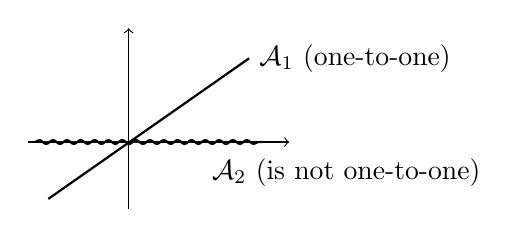
\begin{tikzpicture}[scale=0.85]
\draw[->] (-1.5,0) -- (2.4,0);
\draw[->] (0,-1) -- (0,1.7);
\draw[thick] (-1.2,-0.85) -- (1.8,1.25) node[right] {$\mathcal{A}_1$ (one-to-one)};
\draw[thick,decorate,decoration={snake,amplitude=0.7pt,segment length=5pt}] (-1.4,0) -- (2.0,0);
\node[right] at (1.1,-0.45) {$\mathcal{A}_2$ (is not one-to-one)};
\end{tikzpicture}
\end{center}

\begin{proposition}
A linear transformation $\mathcal{A}:\V\to\W$ is \key{one-to-one iff $\Null(\mathcal{A})=\{0_V\}$}:
\[
\text{one-to-one} \ \iff\ \Null(\mathcal{A})=\{0_V\}
\ \iff\ \dim\Null(\mathcal{A})=0.
\]
\end{proposition}
% note: in the notes, the second equivalence is written as stacked "<= , =>" arrows under the first one.

\needspace{6\baselineskip}
\paragraph{Proof techniques.}
\begin{align*}
&p\Rightarrow q && \text{(constructive proof)}\\
&\bar q\Rightarrow \bar p && \text{(contraposition proof)}\\
&p\wedge \bar q=\text{False} && \text{(contradiction proof)}
\end{align*}

\begin{proof}
We prove the two directions separately.
\paragraph{One-to-one $\Rightarrow \Null(\mathcal{A})=\{0_V\}$.}
We use contraposition ($p\Rightarrow q$ \ $\equiv$ \ $\bar q\Rightarrow \bar p$), i.e.\ we show
\[
\Null(\mathcal{A})\ne\{0_V\} \ \Rightarrow\ \text{not one-to-one.}
\]
\begin{align*}
&\exists x\ne 0_V \text{ s.t. } x\in\Null(\mathcal{A}), \quad\text{i.e. } \mathcal{A}x=0_W.\\
&\text{Let } v_1\in\V \text{ and } v_2=v_1+x\in\V. \quad\text{As } x\ne 0_V \Rightarrow v_2\ne v_1.\\
&\mathcal{A}v_2=\mathcal{A}v_1+\underbrace{\mathcal{A}x}_{0_W}=\mathcal{A}v_1
  \ \Rightarrow\ \mathcal{A} \text{ is not one-to-one.}
\end{align*}
\par
\paragraph{$\Null(\mathcal{A})=\{0_V\}\Rightarrow$ one-to-one.}
Again by contraposition: not one-to-one $\Rightarrow \Null(\mathcal{A})\ne\{0_V\}$.
\begin{align*}
&\exists v_1\ne v_2 \text{ s.t. } \mathcal{A}v_1=\mathcal{A}v_2\\
&\Rightarrow\ \mathcal{A}v_1-\mathcal{A}v_2=0_W\\
&\Rightarrow\ \mathcal{A}(v_1-v_2)=0_W\\
&\Rightarrow\ 0_V\ne v_1-v_2\in\Null(\mathcal{A})\\
&\Rightarrow\ \Null(\mathcal{A})\ne\{0_V\} \qedhere
\end{align*}
\end{proof}
\begin{insight}[Why the null space decides injectivity]
For a linear map, $\mathcal{A}v_1=\mathcal{A}v_2\iff\mathcal{A}(v_1-v_2)=0_W\iff v_1-v_2\in\Null(\mathcal{A})$. So the set of vectors with the same image as $v_1$ is the shifted copy $v_1+\Null(\mathcal{A})$; images are unique exactly when this copy is the single point $v_1$, i.e.\ when $\Null(\mathcal{A})=\{0_V\}$.
\end{insight}

% ===== Page 28 =====
\begin{example}\leavevmode\origpage{28}
$\V=\W=\{\text{polynomials with degree}\le 2\}$, \quad $\mathcal{A}=\dfrac{d}{dt}$. \quad Is $\mathcal{A}$ one-to-one?
\begin{align*}
&\mathcal{A}(at^2+bt+c)=2at+b=0_W=0(t) \ \Rightarrow\ a=0,\ b=0\\
&\Null(\mathcal{A})=\{c\}=\{\text{constant polynomials}\}, \qquad \dim\Null(\mathcal{A})=1\\
&\Null(\mathcal{A})\ne\{0_V\}\ \Rightarrow\ \text{\key{Not one-to-one}}
\end{align*}
\explain{Side note in the notes: $\Range(\mathcal{A})=\{\text{poly.\ degree}\le 1\}=\Span\{1,t\}$ (2 elements, $\dim\Range(\mathcal{A})=2$).}
% corrected: notes had the side note labelled N(A) = {poly degree <= 1}; this is the range of d/dt (cf. p.29), the null space is the constants
\end{example}

\begin{example}\label{ex:integral-not-1-1}
$\V=\{f\mid f:[0,1]\to\R,\ f \text{ is integrable}\}$, \quad $\W=\R$,
\[
\mathcal{A}f=\int_0^1 f(t)\,dt. \qquad\text{Is } \mathcal{A} \text{ one-to-one?}
\]
Take
\[
f(t)=2t-1\ne 0_V, \qquad \mathcal{A}f=\left(t^2-t\right)\Big|_0^1=0.
\]
$\therefore$ \key{Not one-to-one.} \quad ($\dim\Null(\mathcal{A})=\infty$)
\explain{E.g.\ $t^k-\frac{1}{k+1}$, $k=1,2,3,\dots$ all integrate to $0$ and are linearly independent, so the null space is infinite dimensional.}
\end{example}

\needspace{9\baselineskip}
\begin{example}
$\V=\W=\R^2$, \quad $x=\bmat{\alpha_1\\ \alpha_2}$, \quad $\mathcal{A}x=\bmat{\alpha_1\\ \alpha_1+\alpha_2}$. \quad Is $\mathcal{A}$ one-to-one?
\begin{align*}
&\mathcal{A}x=\bmat{0\\0}=\bmat{\alpha_1\\ \alpha_1+\alpha_2} \ \Rightarrow\ \alpha_1=\alpha_2=0\\
&\Null(\mathcal{A})=\left\{\bmat{0\\0}\right\} \ \checkmark \qquad
\cancel{\Null(\mathcal{A})=\bmat{0\\0}}
\end{align*}
\explain{Crossed out: $\Null(\mathcal{A})$ is a subspace (a set), whereas $\left[\begin{smallmatrix}0\\0\end{smallmatrix}\right]$ alone is not a set/subset --- write it inside braces.}
\end{example}

\subsection{Range Space, Onto Transformations and the Rank--Nullity Theorem}\label{ss:range}

\begin{definition}
Let $\mathcal{A}:\V\to\W$ be a linear transformation. The \term{range space} of $\mathcal{A}$ is defined as
\[
\Range(\mathcal{A})\triangleq\{w\in\W\mid \exists v\in\V \text{ s.t. } \mathcal{A}v=w\}.
\]
\end{definition}

\needspace{6\baselineskip}
\begin{claim}
\key{$\Range(\mathcal{A})$ is a subspace of $\W$.}
\end{claim}
\begin{proof}
Let $w_1,w_2\in\Range(\mathcal{A})$. By the definition of range space,
\begin{align*}
&\exists v_1,v_2 \text{ s.t. } \mathcal{A}v_1=w_1, \quad \mathcal{A}v_2=w_2\\
&\mathcal{A}(v_1+v_2)=\mathcal{A}v_1+\mathcal{A}v_2=w_1+w_2 \ \Rightarrow\ w_1+w_2\in\Range(\mathcal{A})\\
&\mathcal{A}(\alpha v_1)=\alpha\mathcal{A}v_1=\alpha w_1 \ \Rightarrow\ \alpha w_1\in\Range(\mathcal{A})
\end{align*}
% corrected: notes had "alpha w_1 = A(alpha v_1) = alpha A v_1 = alpha w_1 in R(A)" (circular chain); rewritten as an implication
$\therefore$ $\Range(\mathcal{A})$ is closed under addition and scalar multiplication, hence \key{a subspace of $\W$}.
\end{proof}

% ===== Page 29 =====
\begin{example}\leavevmode\origpage{29}
$\V=\W=\R$.
\begin{center}
\begin{minipage}{0.36\textwidth}\centering
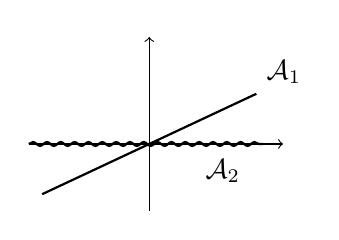
\begin{tikzpicture}[scale=0.85]
\draw[->] (-1.8,0) -- (2,0) node[right] {$\V$};
\draw[->] (0,-1) -- (0,1.6) node[left] {$\W$};
\draw[thick] (-1.6,-0.75) -- (1.6,0.75) node[above right] {$\mathcal{A}_1$};
\draw[thick,decorate,decoration={snake,amplitude=0.7pt,segment length=5pt}] (-1.8,0) -- (1.7,0);
\node at (1.1,-0.4) {$\mathcal{A}_2$};
\end{tikzpicture}
\end{minipage}%
\begin{minipage}{0.6\textwidth}
\begin{align*}
\Null(\mathcal{A}_1)&=\{0\}, & \dim\Null(\mathcal{A}_1)&=0\\
\Null(\mathcal{A}_2)&=\V=\R, & \dim\Null(\mathcal{A}_2)&=1\\
\Range(\mathcal{A}_1)&=\W=\R, & \dim\Range(\mathcal{A}_1)&=1\\
\Range(\mathcal{A}_2)&=\{0\}, & \dim\Range(\mathcal{A}_2)&=0
\end{align*}
\end{minipage}
\end{center}
% corrected: notes had "dim R(A_1) = 0" in the last line; A_2 is meant.
\explain{$\dim\Null(\mathcal{A}_1)+\dim\Range(\mathcal{A}_1)=0+1=1$, \quad $\dim\Null(\mathcal{A}_2)+\dim\Range(\mathcal{A}_2)=1+0=1$.}
\end{example}

\begin{definition}
A linear transformation $\mathcal{A}:\V\to\W$ is called \term{onto} iff \key{$\Range(\mathcal{A})=\W$}; otherwise, if $\Range(\mathcal{A})\ne\W$ (i.e.\ $\Range(\mathcal{A})\subsetneq\W$), $\mathcal{A}$ is called \term{into}.
% corrected: notes had "R(A) \not\subseteq W"; R(A) is always a subset of W, so "proper subset" (\subsetneq) is meant
\end{definition}

\begin{example}
$\V=\W=\{\text{polynomials with degree}\le 2\}$ \ ($\to\dim 3$),
\begin{gather*}
\mathcal{A}=\frac{d}{dt}, \qquad \mathcal{A}(at^2+bt+c)=2at+b.\\[0.4em]
\begin{aligned}
\Null(\mathcal{A})&=\{\text{constant polynomials}\}, &\qquad \dim\Null(\mathcal{A})&=1\\
\Range(\mathcal{A})&=\{\text{polynomials with degree}\le 1\}, & \dim\Range(\mathcal{A})&=2
\end{aligned}
\end{gather*}
$\Range(\mathcal{A})\ne \W \ \Rightarrow\ \therefore$ \key{$\mathcal{A}$ is not onto.}
\explain{Sum: $1+2=3$, the same as $\dim \V$.}
\end{example}

\begin{example}
$\V=\{f\mid f:[0,1]\to\R,\ f \text{ is integrable}\}$, \quad $\W=\R$,
\[
\mathcal{A}f=\int_0^1 f(t)\,dt, \qquad \Range(\mathcal{A})=\R.
\]
\explain{For any $c\in\R$, the constant function $f(t)=c$ gives $\mathcal{A}f=c$, so $\mathcal{A}$ is onto (but not one-to-one, see Example~\ref{ex:integral-not-1-1}).}
\end{example}

\sep
\[
\left.\begin{aligned}
\dim\Null(\mathcal{A}) &\triangleq \text{\term{nullity}}\\
\dim\Range(\mathcal{A}) &\triangleq \text{\term{rank}}
\end{aligned}\right\}\overset{+}{\longrightarrow} \text{constant}
\]

\begin{theorem}[Rank--Nullity Theorem]
If $\V$ is finite dimensional and $\mathcal{A}$ is a linear transformation from $\V$ into $\W$, then $\Range(\mathcal{A})$ is finite dimensional and \key{nullity $+$ rank $=\dim\V$}:
\[
\dim\Null(\mathcal{A})+\dim\Range(\mathcal{A})=\dim\V .
\]
\end{theorem}
\begin{insight}[Proof sketch and consequences]
\begin{proof}[Proof sketch]
Take a basis $\{u_1,\dots,u_r\}$ of $\Null(\mathcal{A})$ and extend it to a basis $\{u_1,\dots,u_r,v_{r+1},\dots,v_n\}$ of $\V$. Then $\Range(\mathcal{A})=\Span\{\mathcal{A}v_{r+1},\dots,\mathcal{A}v_n\}$ (since $\mathcal{A}u_i=0_W$), and these $n-r$ images are linearly independent: $\sum\beta_j\mathcal{A}v_j=0_W\Rightarrow\sum\beta_jv_j\in\Null(\mathcal{A})\Rightarrow$ all $\beta_j=0$. Hence $\dim\Range(\mathcal{A})=n-r$.
\end{proof}
\paragraph{Consequences.} $\mathcal{A}$ one-to-one $\iff$ $\dim\Range(\mathcal{A})=\dim\V$; and if $\dim\V=\dim\W<\infty$, then one-to-one $\iff$ onto. In the examples above: $\frac{d}{dt}$ on polynomials of degree $\le2$: nullity $+$ rank $=1+2=3=\dim\V$, so it is neither one-to-one nor onto.
\end{insight}

\subsection{Matrix Representations}\label{ss:matrix-rep}

\begin{definition}
Let $\V$ ($\dim=n$) and $\W$ ($\dim=m$) be two linear spaces over the same field $\F$.
Let $\mathcal{A}:\V\to\W$ be a linear transformation. Given the bases $B=\{v_1,v_2,\dots,v_n\}$ and $C=\{w_1,w_2,\dots,w_m\}$ for $\V$ and $\W$, the transformation can be represented by a matrix $A=[a_{ij}]$ ($a_{ij}\in\F$), its \term{matrix representation}, such that
\[
[w]_C=A\,[v]_B
\]
for any $w,v$ satisfying $w=\mathcal{A}v$.
\end{definition}
\explain{$A$ is $m\times n$; its $j$th column is the coordinate vector $[\mathcal{A}v_j]_C$ (procedure below). The matrix depends on the chosen bases $B$ and $C$.}

% ===== Page 30 =====
\needspace{16\baselineskip}
\begin{example}\leavevmode\origpage{30}
\begin{align*}
\V&=\{\text{polynomials with degree}\le 3\}, \qquad
\W=\{\text{polynomials with degree}\le 2\}\\
\mathcal{A}&:\V\to\W, \qquad \mathcal{A}f=\frac{df}{dt}\\
B&=\{\underbrace{1}_{v_1},\ \underbrace{1+t}_{v_2},\ \underbrace{1+t+t^2}_{v_3},\ \underbrace{1+t+t^2+t^3}_{v_4}\}\\
C&=\{\underbrace{1}_{w_1},\ \underbrace{1+t}_{w_2},\ \underbrace{1+t+t^2}_{w_3}\}\\
[w]_C&=A\,[v]_B \qquad\text{e.g. } [v]_B=\bmat{1\\0\\0\\0}
\end{align*}

\paragraph{Procedure.}
\begin{enumerate}[label=\arabic*.]
\item Choose $v=v_j$ for $j=1,\dots,n$:
\[
[v]_B=e_j=\bmat{0\\0\\ \vdots\\ 1\\ \vdots\\ 0}\leftarrow j\text{th element}
\]
\explain{$A\,e_j$ picks out the $j$th column of $A$: this gives the first column for $j=1$, and in general the $j$th column.}
\item Find $w=\mathcal{A}v_j$.
\item \key{$j$th column of $A$ is $[\mathcal{A}v_j]_C$.}
\end{enumerate}

\paragraph{Columns of $A$.}
\begin{align*}
v=v_1:\quad [v_1]_B&=\bmat{1\\0\\0\\0}, & \mathcal{A}v_1&=0=0w_1+0w_2+0w_3 &&\Rightarrow\ 1^{\text{st}} \text{ column of } A \text{ is } \bmat{0\\0\\0}\\[4pt]
v=v_2:\quad [v_2]_B&=\bmat{0\\1\\0\\0}, & \mathcal{A}v_2&=1=1w_1+0w_2+0w_3 &&\Rightarrow\ 2^{\text{nd}} \text{ column of } A \text{ is } \bmat{1\\0\\0}\\[4pt]
v=v_3:\quad [v_3]_B&=\bmat{0\\0\\1\\0}, & \mathcal{A}v_3&=2t+1=-w_1+2w_2+0w_3 &&\Rightarrow\ 3^{\text{rd}} \text{ column of } A \text{ is } \bmat{-1\\2\\0}\\[4pt]
v=v_4:\quad [v_4]_B&=\bmat{0\\0\\0\\1}, & \mathcal{A}v_4&=3t^2+2t+1 &&\\*
&& &=-1w_1-1w_2+3w_3 &&\Rightarrow\ 4^{\text{th}} \text{ column of } A \text{ is } \bmat{-1\\-1\\3}
\end{align*}
\[
\boxed{A=\bmat{0&1&-1&-1\\0&0&2&-1\\0&0&0&3}}
\]
\explain{Coordinates in $C$: $2t+1=-1\cdot1+2(1+t)$; $3t^2+2t+1=3(1+t+t^2)-1\cdot(1+t)-1\cdot1$ (match the $t^2$, then $t$, then constant coefficients).}

\sep
% ===== Page 31 =====
\origpage{31}%
\paragraph{Check.} Let $v=t^3+2t^2+3t+4$. Then
\[
[v]_B=\bmat{1\\1\\1\\1}, \qquad [w]_C=A\,[v]_B=\bmat{-1\\1\\3}
\]
\begin{align*}
w&=-w_1+w_2+3w_3\\
&=-1+1+t+3+3t+3t^2=3t^2+4t+3 \ \checkmark
\end{align*}
\explain{Indeed $\frac{d}{dt}(t^3+2t^2+3t+4)=3t^2+4t+3$. ($[v]_B$: $v=1\cdot v_1+1\cdot v_2+1\cdot v_3+1\cdot v_4$, since $v_1+v_2+v_3+v_4=4+3t+2t^2+t^3$.)}
\end{example}

\needspace{14\baselineskip}
\subsection{Change of Basis and Similar Matrices}\label{ss:basis-change-rep}

\needspace{10\baselineskip}
\paragraph{1) Basis change in the domain.} Let $[v]_B=P\,[v]_{\bar B}$.
\begin{align*}
[w]_C&=A\,[v]_B\\
[w]_C&=\bar A\,[v]_{\bar B}\\
[w]_C&=A\cdot P\,[v]_{\bar B}
\end{align*}
\[
\therefore\ \boxed{\bar A=A\cdot P}
\]

\needspace{10\baselineskip}
\paragraph{2) Basis change in the co-domain.} Let $[w]_C=Q\,[w]_{\bar C}$.
\begin{align*}
[w]_C&=A\,[v]_B\\
[w]_{\bar C}&=\bar A\,[v]_B\\
Q\,[w]_{\bar C}&=A\,[v]_B\\
[w]_{\bar C}&=Q^{-1}A\,[v]_B
\end{align*}
\[
\therefore\ \boxed{\bar A=Q^{-1}\cdot A}
\]

\needspace{10\baselineskip}
\paragraph{3) Basis change in both domain and co-domain.} With $[v]_B=P\,[v]_{\bar B}$ and $[w]_C=Q\,[w]_{\bar C}$:
\begin{align*}
[w]_C&=A\,[v]_B\\
[w]_{\bar C}&=\bar A\,[v]_{\bar B}\\
Q\,[w]_{\bar C}&=A\,P\,[v]_{\bar B}\\
[w]_{\bar C}&=Q^{-1}AP\,[v]_{\bar B}
\end{align*}
% corrected: notes had [v]_B (no bar) in the second line; [v]_{\bar B} is meant. The last two lines are added (combine 1) and 2)).
\[
\therefore\ \boxed{\bar A=Q^{-1}AP}
\]

\needspace{9\baselineskip}
\paragraph{Special case.}
If $\V=\W$, $\mathcal{A}$ is a linear transformation from $\V$ into $\V$. Then the basis $B$ can be taken to be the same as $C$. Then a basis change in both the domain and co-domain would give
\[
\therefore\ \boxed{\bar A=P^{-1}AP}
\]
\explain{Here $Q=P$ since the same basis change is applied to domain and co-domain; $A$ and $\bar A$ are then called \term{similar} matrices.}

\begin{example}
\begin{align*}
\V&=\{\text{polynomials with degree}\le 3\}, & B&=\{1,\ 1+t,\ 1+t+t^2,\ 1+t+t^2+t^3\}\\
\W&=\{\text{polynomials with degree}\le 2\}, & C&=\{1,\ 1+t,\ 1+t+t^2\}
\end{align*}
\[
A=\bmat{0&1&-1&-1\\0&0&2&-1\\0&0&0&3}
\]

% ===== Page 32 =====
\begin{enumerate}[label=\arabic*.]
\item\leavevmode\origpage{32}Change the basis in the domain to $\bar B=\{1,t,t^2,t^3\}$:
\[
\bar A=AP, \qquad [v]_B=P\,[v]_{\bar B}
\]
\[
P=\bmat{1&-1&0&0\\0&1&-1&0\\0&0&1&-1\\0&0&0&1},
\qquad
\bar A=AP=\bmat{0&1&-2&0\\0&0&2&-3\\0&0&0&3}
\]
\explain{Column $j$ of $P$ is $[\bar v_j]_B$: $1=v_1$, $t=v_2-v_1$, $t^2=v_3-v_2$, $t^3=v_4-v_3$. Check of $\bar A$: $\frac{d}{dt}t^2=2t=-2\cdot1+2(1+t)$ and $\frac{d}{dt}t^3=3t^2=3(1+t+t^2)-3(1+t)$, matching columns 3 and 4.}
\item Change the basis in the co-domain to the canonical basis $\bar C=\{1,t,t^2\}$, while keeping the canonical basis $\bar B$ in the domain:
\begin{align*}
[w]_{\bar C}&=\bar{\bar A}\,[v]_{\bar B}\\
\bar{\bar A}&=Q^{-1}\bar A, && [w]_C=Q\,[w]_{\bar C}\\
\bar{\bar A}&=Q^{-1}\bar A, && R\,[w]_C=[w]_{\bar C}\\
\bar{\bar A}&=R\bar A, && [w]_{\bar C}=R\,[w]_C
\end{align*}
% corrected: notes had the first "\bar{\bar A} = Q^{-1}\bar A" line with a single bar on the left (double bar meant).
\[
R=\bmat{1&1&1\\0&1&1\\0&0&1}=Q^{-1},
\qquad
\bar{\bar A}=\bmat{0&1&0&0\\0&0&2&0\\0&0&0&3}
\]
\explain{$Q^{-1}\bar A$ $\Rightarrow$ linear combinations of rows of $\bar A$ (row 1 $=$ rows $1+2+3$, row 2 $=$ rows $2+3$, row 3 unchanged). Column $j$ of $R$ is $[w_j]_{\bar C}$: $1$, $1+t$, $1+t+t^2$.}
\begin{insight}[Check]
$\bar{\bar A}$ is the matrix of $\frac{d}{dt}$ in the canonical bases: $1\mapsto0$, $t\mapsto1$, $t^2\mapsto2t$, $t^3\mapsto3t^2$, which gives exactly the columns $\bmat{0\\0\\0},\bmat{1\\0\\0},\bmat{0\\2\\0},\bmat{0\\0\\3}$. Altogether $\bar{\bar A}=Q^{-1}AP=RAP$.
\end{insight}
\end{enumerate}
\end{example}

% Section 5: Direct Sums and Orthogonal Projections  (original handwritten pages 33--42)
\section{Direct Sums and Orthogonal Projections}\label{sec:direct-sum}
\syllabusweek{Week 6 --- direct sum decompositions, projection theorem, orthogonal projections}

\subsection{Direct Sums}\label{ss:direct-sums}

\begin{definition}
Let $\V$ be a vector space and let $M_1,\dots,M_k$ be subspaces of $\V$. The \term{sum} of these subspaces is defined as
\[
M=M_1+M_2+\dots+M_k=\{m\in\V \mid m=m_1+m_2+\dots+m_k,\ m_i\in M_i\ \forall i\}.
\]
The subspaces are called \term{linearly independent} iff
\[
m_1+m_2+\dots+m_k=0_V \quad\text{where } m_i\in M_i\ \forall i
\quad\Rightarrow\quad m_1=m_2=\dots=m_k=0_V .
\]
\end{definition}

\begin{center}
\begin{minipage}{0.42\textwidth}\centering
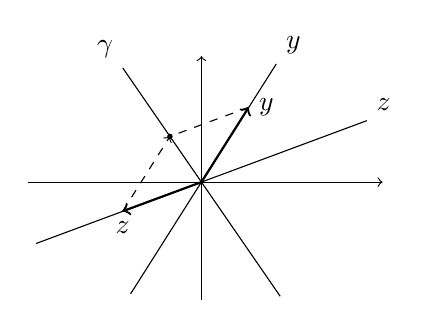
\begin{tikzpicture}[scale=1.0]
% axes
\draw[->] (-2.2,0) -- (2.3,0);
\draw[->] (0,-1.5) -- (0,1.6);
% subspaces (lines through the origin)
\draw (-0.9,-1.42) -- (0.95,1.5) node[above right] {$y$};
\draw (-2.1,-0.78) -- (2.1,0.78) node[above right] {$z$};
\draw (-1.0,1.45) -- (1.0,-1.45);
\node[above left] at (-1.0,1.45) {$\gamma$};
% vectors y, z and y+z = gamma
\draw[->,thick] (0,0) -- (0.6,0.95) node[right] {$y$};
\draw[->,thick] (0,0) -- (-1.0,-0.37) node[below] {$z$};
\draw[->,dashed] (-1.0,-0.37) -- (-0.4,0.58);
\draw[dashed] (0.6,0.95) -- (-0.4,0.58);
\fill (-0.4,0.58) circle (1pt);
\end{tikzpicture}
\end{minipage}%
\begin{minipage}{0.4\textwidth}
$y+z-\gamma=0$\\
$\Rightarrow$ not linearly independent
\end{minipage}
\end{center}

% ===== Page 33 =====
\begin{remark}\leavevmode\origpage{33}
Let $\V=M_1+M_2+\dots+M_k$ and let $M_1,\dots,M_k$ be linearly independent. Then for $x\in\V$,
\[
x=m_1+m_2+\dots+m_k, \qquad m_i\in M_i\ \forall i,
\]
\key{$m_1,m_2,\dots,m_k$ are unique.}
\end{remark}

\begin{proof}
Assume $m_1,\dots,m_k$ are not unique, i.e.\ there is an $i$ such that $m_i\ne\bar m_i$:
\begin{align*}
x&=m_1+\dots+m_k\\
x&=\bar m_1+\dots+\bar m_k\\
0_V&=\underbrace{(m_1-\bar m_1)}_{\in M_1}+\underbrace{(m_2-\bar m_2)}_{\in M_2}+\dots+\underbrace{(m_k-\bar m_k)}_{\in M_k}
\end{align*}
$\Rightarrow M_1,\dots,M_k$ are not linearly independent. \qedhere
\end{proof}

\begin{definition}
Let $M_1,\dots,M_k$ be subspaces of $\V$. Let
\begin{enumerate}[label=\roman*-)]
\item $M=M_1+M_2+\dots+M_k$.
\item $M_1,M_2,\dots,M_k$ are linearly independent.
\end{enumerate}
Then $M$ is said to be the \term{direct sum} of $M_1,\dots,M_k$. This is shown as
\[
M=M_1\oplus M_2\oplus\dots\oplus M_k .
\]
\end{definition}

\begin{example}
$\V=\R^4$, \quad $x=(x_1,x_2,x_3,x_4)^T\in\R^4$.
\begin{alignat*}{3}
M_1&\triangleq\{x\in\R^4\mid x_4=x_3=0\}: &\quad &\bmat{x_1\\x_2\\0\\0}, &\quad \dim&=2\\
M_2&\triangleq\{x\in\R^4\mid x_1=x_2=0\}: & &\bmat{0\\0\\x_3\\x_4}, & \dim&=2\\
M_3&\triangleq\{x\in\R^4\mid x_1=0\}: & &\bmat{0\\x_2\\x_3\\x_4}, & \dim&=3
\end{alignat*}
\begin{align*}
M_1+M_2&=\R^4 && \Rightarrow \text{direct sum: } M_1\,\&\,M_2 \text{ linearly independent} \Rightarrow M_1\oplus M_2=\R^4\\
M_1+M_3&=\R^4 && \Rightarrow \text{not direct sum}\\
M_2+M_3&=M_3 && \Rightarrow \text{not direct sum } (M_2\subset M_3)
\end{align*}

\sep
For $M_1$ and $M_3$:
\[
\bmat{x_1\\x_2\\0\\0}+\bmat{0\\x_2'\\x_3'\\x_4'}=\bmat{0\\0\\0\\0},
\qquad\text{e.g.}\qquad
\underset{\in M_1}{\bmat{0\\1\\0\\0}}+\underset{\in M_3}{\bmat{0\\-1\\0\\0}}=\underset{0_V}{\bmat{0\\0\\0\\0}}
\]
As the two summands are nonzero, $M_1\,\&\,M_3$ are linearly dependent.\\
$\therefore$ \key{$M_1+M_3$ is not a direct sum.}

$M_2\,\&\,M_3$ are linearly dependent (e.g.\ $m_2=(0,0,1,0)^T\in M_2$, $m_3=-m_2\in M_3$).\\
$\therefore$ \key{$M_2+M_3$ is not a direct sum.}
\begin{insight}[Dimension test]
For two subspaces, $M_1+M_2$ is direct $\iff M_1\cap M_2=\{0_V\}\iff\dim(M_1+M_2)=\dim M_1+\dim M_2$. Here: $M_1\cap M_2=\{0\}$ and $2+2=4$ (direct); $M_1\cap M_3=\{(0,x_2,0,0)^T\}$, $2+3=5\ne4$ (not direct); $M_2\cap M_3=M_2$, $2+3\ne3$ (not direct).
\end{insight}
\end{example}

% ===== Page 34 =====
\subsection{Orthogonal Direct Sums and Orthogonal Complements}\label{ss:orth-complement}

\begin{definition}\leavevmode\origpage{34}
Let $\V$ be an inner product space. Two subspaces $M_1\,\&\,M_2$ are said to be \term{orthogonal} iff
\[
\inner{m_1}{m_2}=0 \qquad \forall m_1\in M_1,\ \forall m_2\in M_2 .
\]
We denote this $M_1\perp M_2$.
\end{definition}
% corrected: notes had "M_2 & M_2" in the first line; M_1 & M_2 meant.

\needspace{8\baselineskip}
\begin{definition}
Let $M$ be equal to $M_1+M_2+\dots+M_k$ and $M_i\perp M_j$ for $i\ne j$. Then $M$ is said to be an \term{orthogonal direct sum} of $M_1,\dots,M_k$. We show this as
\[
M=M_1\overset{\perp}{\oplus}M_2\overset{\perp}{\oplus}\dots\overset{\perp}{\oplus}M_k .
\]
If $M=\V$ then
\[
\V=M_1\overset{\perp}{\oplus}M_2\overset{\perp}{\oplus}\dots\overset{\perp}{\oplus}M_k
\]
is called an \term{orthogonal direct sum decomposition} of $\V$.
\end{definition}

\begin{claim}
\key{Orthogonality implies linear independence.}
\end{claim}
\begin{proof}
Let $\sum_{i=1}^{k}m_i=0_V$, \ $m_i\in M_i$. Then
\begin{align*}
\Big\langle\sum_{i=1}^{k}m_i,\,m_j\Big\rangle&=\inner{0_V}{m_j}=0\\
\sum_{i=1}^{k}\inner{m_i}{m_j}&=0
\end{align*}
Since $\inner{m_i}{m_j}=0$ when $i\ne j$:
\[
\inner{m_j}{m_j}=0 \ \Rightarrow\ m_j=0_V .
\]
\explain{The last step uses positive definiteness of the inner product. Since $j$ was arbitrary, all $m_j=0_V$: orthogonality implies linear independence.}
\end{proof}

\begin{definition}
Let $M$ be a subspace of an inner product space $\V$. The \term{orthogonal complement} $M^\perp$ of the subspace is defined as
\[
M^\perp=\{x\in\V\mid \inner{x}{m}=0\ \forall m\in M\}.
\]
\end{definition}
The zero vector is orthogonal to every vector, so $0_V\in M^\perp$ always. Two examples:

\begin{center}
\begin{minipage}{0.34\textwidth}\centering
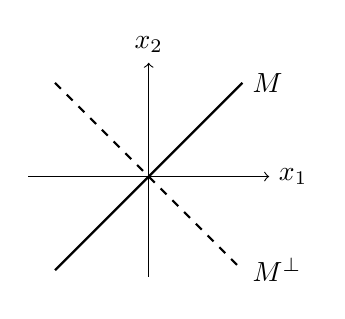
\begin{tikzpicture}[scale=0.85]
\draw[->] (-1.8,0) -- (1.8,0) node[right] {$x_1$};
\draw[->] (0,-1.5) -- (0,1.7) node[above] {$x_2$};
\draw[thick] (-1.4,-1.4) -- (1.4,1.4) node[right] {$M$};
\draw[thick,dashed] (-1.4,1.4) -- (1.4,-1.4) node[right] {$M^\perp$};
\end{tikzpicture}
\end{minipage}%
\begin{minipage}{0.6\textwidth}
\begin{align*}
M&=\Span\left\{\bmat{1\\1}\right\}, & \bmat{-1\\1}&\in M^\perp, \quad \bmat{2\\-2}\in M^\perp\\
M^\perp&=\Span\left\{\bmat{-1\\1}\right\}, & M+M^\perp&=M\overset{\perp}{\oplus}M^\perp
\end{align*}
\end{minipage}
\end{center}
\begin{center}
\begin{minipage}{0.3\textwidth}\centering
\begin{tikzpicture}[scale=0.85]
\fill[pattern=vertical lines, pattern color=gray!70] (-0.2,0) -- (2,0) -- (1.2,-1.2) -- (-1.0,-1.2) -- cycle;
\draw[->] (0,0) -- (0,2) node[above] {$z$};
\draw[->] (0,0) -- (2.3,0) node[right] {$y$};
\draw[->] (0,0) -- (-0.95,-1.45) node[below left] {$x$};
\node at (1.25,-0.75) {$M$};
\node[right] at (0,1.4) {$M^\perp$};
\end{tikzpicture}
\end{minipage}%
\begin{minipage}{0.55\textwidth}
\begin{align*}
M&=\{x\text{-}y \text{ plane}\}\\
M^\perp&=\{z \text{ axis}\}\\
\underset{\dim=2}{M}\overset{\perp}{\oplus}\underset{\dim=1}{M^\perp}&=\underset{\dim 3}{\R^3}
\end{align*}
\end{minipage}
\end{center}
Orthogonality implies linear independence, thus this is a direct sum; since the summands are also orthogonal, it is an orthogonal direct sum.

\needspace{9\baselineskip}
\begin{claim}
\key{$M^\perp$ is a subspace of $\V$.}
\end{claim}
\begin{proof}
Let $x,y\in M^\perp$, i.e.\ $\inner{x}{m}=0$, $\inner{y}{m}=0$ $\forall m\in M$. Then
\begin{align*}
\inner{x+y}{m}&=\underbrace{\inner{x}{m}+\inner{y}{m}}_{0} \quad (m\in M)\\
&=0 \quad \forall m\in M &&\Rightarrow\ x+y\in M^\perp\\
\inner{\alpha x}{m}&=\alpha\inner{x}{m}=0 \quad\forall m\in M &&\Rightarrow\ \alpha x\in M^\perp
\end{align*}
$\therefore$ $M^\perp$ is closed under addition and scalar multiplication, hence a subspace of $\V$.
\end{proof}

% ===== Page 35 =====
\begin{theorem}[Orthogonal decomposition]\leavevmode\origpage{35}
Let $\V$ be an inner product space and $M$ a subspace of $\V$. Then \key{$\V$ is the orthogonal direct sum of $M$ and $M^\perp$}:
\[
\boxed{\V=M\overset{\perp}{\oplus}M^\perp}
\]
To prove this we check:
\begin{itemize}[nosep]
\item $\V=M+M^\perp$ \ (to be shown, proof below);
\item $M\,\&\,M^\perp$ are linearly independent \ $\checkmark$;
\item $M\perp M^\perp$ \ $\checkmark$.
\end{itemize}
\end{theorem}

\begin{proof}
It remains to show $\V=M+M^\perp$.

\paragraph{Part I.} $\dim M=n\triangleq\dim\V \Rightarrow M=\V$ \ \textcircled{?}\par
\explain{Answer to \textcircled{?}: a basis of $M$ consists of $n$ linearly independent vectors of $\V$; in an $n$-dimensional space any $n$ independent vectors form a basis, so they span $\V$ and $M=\V$.}

\begin{center}
\begin{minipage}{0.25\textwidth}\centering
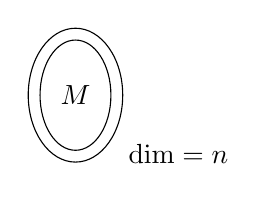
\begin{tikzpicture}
\draw (0,0) ellipse (0.6 and 0.85);
\draw (0,0) ellipse (0.45 and 0.7);
\node at (0,0) {$M$};
\node[right] at (0.55,-0.75) {$\dim\V=n$};
\end{tikzpicture}
\end{minipage}%
\begin{minipage}{0.6\textwidth}
\begin{align*}
M^\perp&=\V^\perp=\{0_V\}\\
\V&=M+M^\perp\\
x&=\underset{\in M}{x_1}+\underset{\in M^\perp}{x_2}
\ \Rightarrow\ x=\underset{\in M}{x}+\underset{\in M^\perp}{0_V} \quad\checkmark
\end{align*}
\end{minipage}
\end{center}

\paragraph{Part II.} $\dim M<n$, with $\dim M = k$. Let
\begin{align*}
B&=\{m_1,m_2,m_3,\dots,m_k\} && \text{(basis for } M)\\
C&=\{m_1,m_2,\dots,m_k,m_{k+1},\dots,m_n\} && \text{(basis for } \V)
\end{align*}
Apply Gram--Schmidt orthogonalization to $C$:
\[
\bar C=\{\underbrace{\underset{\uparrow\, m_1}{e_1},e_2,\dots,e_k}_{\text{form a basis for } M},\ \overbrace{e_{k+1},\dots,e_n}^{\text{basis for } M^\perp}\},
\qquad
\Span\{e_1,\dots,e_k\}=\Span\{m_1,\dots,m_k\}.
\]
$\bar C$ is a basis for $\V$. For $x\in\V$:
\[
x=\sum_{i=1}^{n}\alpha_ie_i=\underbrace{\sum_{i=1}^{k}\alpha_ie_i}_{x_1\in M}+\underbrace{\sum_{j=k+1}^{n}\alpha_je_j}_{x_2\in M^\perp}
\]
\explain{$x_2\in M^\perp$ by construction: Gram--Schmidt makes each $e_j$ ($j>k$) orthogonal to $e_1,\dots,e_k$, which span $M$; hence $e_j\perp m$ for all $m\in M$, and so is every combination of them.}
\[
\Rightarrow\ x=\underset{\in M}{x_1}+\underset{\in M^\perp}{x_2}\ \Rightarrow\ \V=M+M^\perp \qedhere
\]
\end{proof}
\begin{insight}[The remaining two items]
The other two items are immediate: $M\perp M^\perp$ by the definition of $M^\perp$, and orthogonality implies linear independence (shown above), equivalently $M\cap M^\perp=\{0_V\}$ since $x\in M\cap M^\perp\Rightarrow\inner{x}{x}=0$. Consequently $\dim M^\perp=\dim\V-\dim M$, and $\{e_{k+1},\dots,e_n\}$ is in fact a basis of $M^\perp$. (Finite dimension of $\V$ is assumed in the proof.)
\end{insight}

\begin{example}
$\V=\R^4$,
\[
M=\Span\left\{\bmat{1\\2\\3\\4},\bmat{4\\3\\2\\1}\right\}. \qquad \text{Find a basis for } M^\perp.
\]
Complete the basis of $M$ with two canonical vectors to a basis of $\R^4$ and orthogonalize:
\[
C=\Big\{\underset{m_1}{\bmat{1\\2\\3\\4}},\ \underset{m_2}{\bmat{4\\3\\2\\1}},\ \underset{m_3}{\bmat{1\\0\\0\\0}},\ \underset{m_4}{\bmat{0\\1\\0\\0}}\Big\}
\ \xrightarrow{\text{Gram--Schmidt}}\ \bar C=\{e_1,e_2,e_3,e_4\}
\]
% corrected: notes labelled the un-orthogonalized vectors [1,0,0,0], [0,1,0,0] themselves as e_3, e_4 and wrote M^perp = sp{e_3,e_4};
% these vectors are NOT orthogonal to M (e.g. <[1,0,0,0],m_1> = 1). The last vector is cramped in the scan (could be read as 0,1,3);
% [0,1,0,0] is the reading used. The Gram--Schmidt computation below is added and verified with exact (Fraction) arithmetic.
\begin{align*}
e_1&=m_1=\bmat{1\\2\\3\\4}, \qquad \inner{e_1}{e_1}=30\\
e_2&=m_2-\frac{\inner{m_2}{e_1}}{\inner{e_1}{e_1}}e_1=\bmat{4\\3\\2\\1}-\frac{20}{30}\bmat{1\\2\\3\\4}=\frac53\bmat{2\\1\\0\\-1}\ \to\ \bmat{2\\1\\0\\-1}\\
e_3&=m_3-\frac{\inner{m_3}{e_1}}{\inner{e_1}{e_1}}e_1-\frac{\inner{m_3}{e_2}}{\inner{e_2}{e_2}}e_2
 =\bmat{1\\0\\0\\0}-\frac{1}{30}\bmat{1\\2\\3\\4}-\frac{2}{6}\bmat{2\\1\\0\\-1}=\frac1{10}\bmat{3\\-4\\-1\\2}\ \to\ \bmat{3\\-4\\-1\\2}\\
e_4&=m_4-\frac{\inner{m_4}{e_1}}{\inner{e_1}{e_1}}e_1-\frac{\inner{m_4}{e_2}}{\inner{e_2}{e_2}}e_2-\frac{\inner{m_4}{e_3}}{\inner{e_3}{e_3}}e_3\\
 &=\bmat{0\\1\\0\\0}-\frac{2}{30}\bmat{1\\2\\3\\4}-\frac{1}{6}\bmat{2\\1\\0\\-1}+\frac{4}{30}\bmat{3\\-4\\-1\\2}=\frac16\bmat{0\\1\\-2\\1}\ \to\ \bmat{0\\1\\-2\\1}
\end{align*}
\explain{Scaling a vector does not affect orthogonality, so after each step the vector is rescaled to integer entries ($\to$) and the scaled version is used in the following steps.}
\[
\boxed{M^\perp=\Span\{e_3,e_4\}=\Span\left\{\bmat{3\\-4\\-1\\2},\bmat{0\\1\\-2\\1}\right\}}
\]
\begin{insight}[Verification]
$\inner{e_3}{m_1}=3-8-3+8=0$, \ $\inner{e_3}{m_2}=12-12-2+2=0$, \ $\inner{e_4}{m_1}=2-6+4=0$, \ $\inner{e_4}{m_2}=3-4+1=0$, \ and $\inner{e_3}{e_4}=-4+2+2=0$. Since $e_3,e_4\ne0$, the set $C$ was indeed a basis of $\R^4$.

Alternatively,
\[
x\in M^\perp\iff\bmat{1&2&3&4\\4&3&2&1}x=0, \qquad\text{i.e.}\qquad M^\perp=\Null\!\left(\bmat{1&2&3&4\\4&3&2&1}\right),
\]
which has dimension $4-2=2$ and is spanned e.g.\ by $(1,-2,1,0)^T$ and $(0,1,-2,1)^T$; note $(3,-4,-1,2)^T=3(1,-2,1,0)^T+2(0,1,-2,1)^T$, so both answers describe the same subspace. Gram--Schmidt additionally gives an \emph{orthogonal} basis.
\end{insight}
\end{example}

% ===== Page 36 =====
\subsection{The Projection Theorem}\label{ss:projection-thm}
\begin{theorem}[Hilbert's Projection Theorem]
Let $H$ be a Hilbert space\origpage{36} and let $M$ be a finite dimensional subspace of $H$.
For any $x\in H$ the following minimization problem has a solution:
\[
m^* = \arg\min_{m\in M} \norm{x-m}^{2}
\]
\begin{itemize}[nosep]
  \item the exponent $2$ does not matter, the norm is positive;
  \item $\norm{\cdot}$ is the norm induced by the inner product.
\end{itemize}
In other words, we can find the closest vector $m^*$ to $x$ lying in the subspace $M$.
If $m^*$ is a solution, then \key{$x-m^*$ is orthogonal to $M$}.
Furthermore, \key{the solution $m^*$ is unique}:
\[
m^* = \operatorname{Proj}_M x : \text{ ``\term{Orthogonal Projection} of $x$ onto $M$''}
\]
\end{theorem}

\needspace{12\baselineskip}
\explain{Reminder on $\arg\min$ vs.\ $\min$ (left), and the geometry of the theorem (right).}
\begin{center}
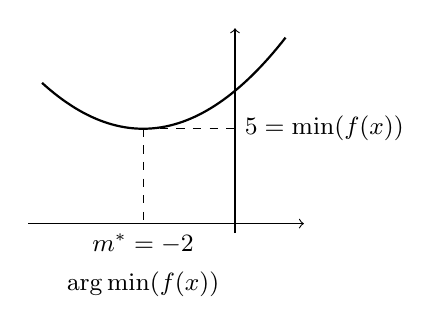
\begin{tikzpicture}
\begin{axis}[
  width=5.2cm, height=4.4cm,
  axis lines=none,
  xmin=-4.6, xmax=1.6, ymin=-1.2, ymax=10.5,
  clip=false]
  \draw[->] (axis cs:-4.5,0) -- (axis cs:1.5,0);
  \draw[->] (axis cs:0,-0.5) -- (axis cs:0,10.3);
  \addplot[thick,domain=-4.2:1.1,samples=60] {0.5*(x+2)^2+5};
  \draw[dashed] (axis cs:-2,5) -- (axis cs:0,5);
  \draw[dashed] (axis cs:-2,5) -- (axis cs:-2,0);
  \node[right,font=\small] at (axis cs:0,5) {$5=\min(f(x))$};
  \node[below,font=\small] at (axis cs:-2,0) {$m^*=-2$};
  \node[font=\small] at (axis cs:-2,-3.2) {$\arg\min(f(x))$};
\end{axis}
\end{tikzpicture}
\qquad\qquad
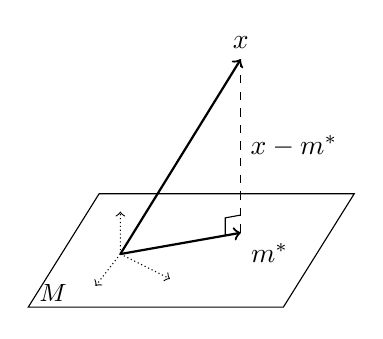
\begin{tikzpicture}[scale=0.9]
  % projection onto plane M
  \draw (0,0) -- (3.6,0) -- (4.6,1.6) -- (1,1.6) -- cycle;
  \node at (0.35,0.2) {\small $M$};
  \coordinate (O) at (1.3,0.75);
  \coordinate (P) at (3.0,1.05);
  \coordinate (X) at (3.0,3.5);
  \draw[->,thick] (O) -- (X) node[above] {$x$};
  \draw[->,thick] (O) -- (P) node[below right] {$m^*$};
  \draw[dashed] (P) -- (X) node[midway,right] {$x-m^*$};
  \draw (3.0,1.3) -- (2.78,1.26) -- (2.78,1.01);
  \draw[->,densely dotted] (O) -- (1.3,1.35);
  \draw[->,densely dotted] (O) -- (0.95,0.3);
  \draw[->,densely dotted] (O) -- (2.0,0.4);
\end{tikzpicture}
\end{center}
Hence:
\begin{itemize}[nosep]
  \item a solution exists;
  \item the solution is unique;
  \item $x-m^*\perp M$.
\end{itemize}

\needspace{14\baselineskip}
\sep
\begin{keybox}[width=0.45\linewidth]
$H = M\overset{\perp}{\oplus} M^\perp, \qquad
x = \underbrace{x_1}_{\in M} + \underbrace{x_2}_{\in M^\perp}$
\end{keybox}
\begin{proof}
For any $m\in M$:
\begin{align*}
\norm{x-m}^2 &= \inner{x-m}{x-m} = \inner{x_1+x_2-m}{x_1+x_2-m}\\
&= \big\langle \underbrace{(\underset{\in M}{x_1}-\underset{\in M}{m})}_{\in M} + \underset{\in M^\perp}{x_2},\; (x_1-m)+x_2 \big\rangle\\
&= \inner{x_1-m}{x_1-m} + \underbrace{\inner{\underset{\in M}{x_1-m}}{\underset{\in M^\perp}{x_2}}}_{0} + \underbrace{\inner{x_2}{x_1-m}}_{0} + \inner{x_2}{x_2}\\
&= \norm{x_1-m}^2 + \norm{x_2}^2\\[4pt]
&\boxed{m^*=x_1} \text{ to minimize this}
\qquad\Longrightarrow\qquad
\boxed{\therefore\ \min \norm{x-m} = \norm{x_2}}
\end{align*}
\begin{itemize}[nosep]
  \item $x_1$ exists;
  \item $x_1$ is unique, as $M\oplus M^\perp$ is a direct sum;
  \item $x-m^* = x-x_1 = x_2\in M^\perp$. \qedhere
\end{itemize}
\end{proof}

\begin{insight}[Why the proof works]
The key identity is the Pythagorean theorem $\norm{x-m}^2 = \norm{x_1-m}^2 + \norm{x_2}^2$, valid because
$x_1-m\in M$ and $x_2\in M^\perp$ are orthogonal. The second term does not depend on $m$, and the first one is
$\ge 0$ with equality \emph{only} for $m=x_1$; this gives existence and uniqueness at once.
The decomposition $H = M\oplus M^\perp$ itself exists because $M$ is finite dimensional: take an orthonormal
basis $\{e_1,\dots,e_k\}$ of $M$ (Gram--Schmidt) and set $x_1=\sum_i \inner{x}{e_i}e_i$, $x_2 = x-x_1$;
then $\inner{x_2}{e_j} = \inner{x}{e_j}-\inner{x}{e_j} = 0$ for every $j$, so $x_2\in M^\perp$.
\end{insight}

\begin{note}
$\V = M^\perp \overset{\perp}{\oplus} M$, \quad $x\in \V$, \quad $x\notin M$.
\[
\R^2 = x\text{ axis} \overset{\perp}{\oplus} y \text{ axis}, \qquad
\R^2 = \underbrace{\Span\left\{\bmat{1\\0}\right\}}_{M} \overset{\perp}{\oplus} \underbrace{\Span\left\{\bmat{0\\1}\right\}}_{M^\perp}
\]
\begin{center}
\begin{tikzpicture}[scale=0.55,baseline=(current bounding box.center)]
  \draw[thick] (-2,0) -- (2.5,0) node[right] {$M$};
  \draw[thick] (0,-2) -- (0,2.5) node[above] {$M^\perp$};
\end{tikzpicture}
\qquad\qquad
$\displaystyle \bmat{1\\2} = \underbrace{\bmat{1\\0}}_{\in M} + \underbrace{\bmat{0\\2}}_{\in M^\perp}$
\end{center}
If a vector is not in $M$, it does not directly mean that it should be inside $M^\perp$. The vector can be written using $M$ and $M^\perp$.
\end{note}

% ===== Page 37 =====
\origpage{37}
\[
x\in M \;\Rightarrow\; m^* = \operatorname{Proj}_M x = x,
\qquad
x = \underbrace{x_1}_{x} + \underbrace{x_2}_{0}: \quad \text{if } x\in M \;\Rightarrow\; \operatorname{Proj}_{M^\perp} x = 0
\]

\begin{example}
$\V=\R^2$, \quad $M=\Span\left\{\bmat{1\\1}\right\}$, \quad $\inner{x}{y} = y\T x$, \quad
$x = \bmat{1\\2}$, \quad $m^* = \operatorname{Proj}_M x$.
\[
m = \alpha\bmat{1\\1} \;\Rightarrow\; m^* = \alpha^*\bmat{1\\1}, \qquad (x-m^*)\perp M
\]
\begin{minipage}[c]{0.56\linewidth}
\begin{align*}
x-m^* = \left(\bmat{1\\2} - \alpha^*\bmat{1\\1}\right) &\perp \bmat{1\\1}\\
\bmat{1-\alpha^*\\ 2-\alpha^*} &\perp \bmat{1\\1}\\
1-\alpha^* + 2-\alpha^* = 0 &\;\Rightarrow\; \alpha^* = \tfrac{3}{2}\\[4pt]
&\boxed{m^* = \frac{3}{2}\bmat{1\\1}}
\end{align*}
\end{minipage}\hfill
\begin{minipage}[c]{0.4\linewidth}
\centering
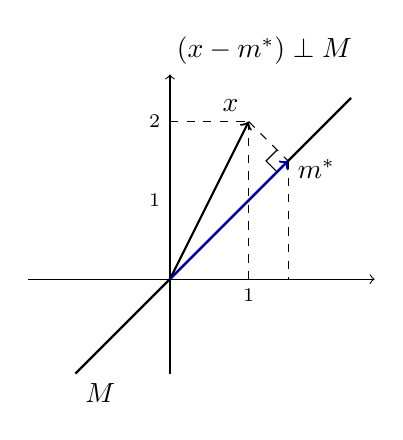
\begin{tikzpicture}[scale=1.0]
  \draw[->] (-1.8,0) -- (2.6,0);
  \draw[->] (0,-1.2) -- (0,2.6);
  \draw[thick] (-1.2,-1.2) -- (2.3,2.3);
  \node[below right] at (-1.2,-1.2) {$M$};
  \node[left] at (0,2) {\scriptsize 2};
  \node[left] at (0,1) {\scriptsize 1};
  \node[below] at (1,0) {\scriptsize 1};
  \draw[->,thick] (0,0) -- (1,2) node[above left] {$x$};
  \draw[dashed] (0,2) -- (1,2);
  \draw[dashed] (1,2) -- (1,0);
  \draw[->,thick,blue!60!black] (0,0) -- (1.5,1.5);
  \node[right] at (1.5,1.4) {$m^*$};
  \draw[dashed] (1,2) -- (1.5,1.5);
  \draw[dashed] (1.5,1.5) -- (1.5,0);
  \draw (1.36,1.36) -- (1.22,1.5) -- (1.36,1.64);
  \node[above] at (1.2,2.6) {$(x-m^*)\perp M$};
\end{tikzpicture}
\end{minipage}
\explain{Check: $x-m^* = \bmat{-1/2 & 1/2}\T$ and $\bmat{-1/2 & 1/2}\bmat{1 & 1}\T = 0$; the distance from $x$ to $M$ is $\norm{x-m^*} = 1/\sqrt2$.}
\end{example}

\begin{example}
Projection onto the span of one or two vectors.

\paragraph{Case 1: one spanning vector.} $\V$, \quad $M=\Span\{v_1\}$.
\[
m^* = \operatorname{Proj}_M x = \,? \qquad m^* = \alpha^* v_1, \qquad x-m^* = (x-\alpha^* v_1)\perp v_1
\]
Hence
\begin{align*}
\inner{x-\alpha^* v_1}{v_1} &= 0\\
\inner{x}{v_1} - \alpha^*\inner{v_1}{v_1} &= 0\\
\Rightarrow\quad \alpha^* &= \frac{\inner{x}{v_1}}{\inner{v_1}{v_1}}, \qquad m^* = \frac{\inner{x}{v_1}}{\inner{v_1}{v_1}}\cdot v_1
\end{align*}

\paragraph{Case 2: two spanning vectors.} $\V$, \quad $M=\Span\{v_1,v_2\}$.
\begin{align*}
m^* &= \operatorname{Proj}_M x = \,?\\
m^* &= \alpha_1^* v_1 + \alpha_2^* v_2\\
(x-\alpha_1^* v_1 - \alpha_2^* v_2)\perp M &\;\Rightarrow\; (x-\alpha_1^* v_1-\alpha_2^* v_2)\perp v_1 \text{ and } v_2
\end{align*}
Taking inner products with $v_1$ and $v_2$:
\begin{align*}
\inner{x-\alpha_1^* v_1-\alpha_2^* v_2}{v_1} = 0 &\;\Rightarrow\; \inner{v_1}{v_1}\alpha_1^* + \inner{v_2}{v_1}\alpha_2^* = \inner{x}{v_1}\\
\inner{x-\alpha_1^* v_1-\alpha_2^* v_2}{v_2} = 0 &\;\Rightarrow\; \inner{v_1}{v_2}\alpha_1^* + \inner{v_2}{v_2}\alpha_2^* = \inner{x}{v_2}
\end{align*}
In matrix form:
\begin{gather*}
\underbrace{\bmat{\inner{v_1}{v_1} & \inner{v_2}{v_1}\\[2pt] \inner{v_1}{v_2} & \inner{v_2}{v_2}}}_{\substack{G\\ \text{Gram matrix}}}
\underbrace{\bmat{\alpha_1^*\\ \alpha_2^*}}_{\alpha^*}
= \underbrace{\bmat{\inner{x}{v_1}\\ \inner{x}{v_2}}}_{b}
\qquad\Longrightarrow\qquad
G\cdot\alpha^* = b, \quad \boxed{\alpha^* = G^{-1}\cdot b}
\end{gather*}

% ===== Page 38 =====
\needspace{5\baselineskip}
The determinant of $G$:\origpage{38}
\begin{align*}
\det G &= \inner{v_1}{v_1}\inner{v_2}{v_2} - \inner{v_1}{v_2}\underbrace{\inner{v_2}{v_1}}_{\overline{\inner{v_1}{v_2}}}\\*
&= \inner{v_1}{v_1}\inner{v_2}{v_2} - \abs{\inner{v_1}{v_2}}^2
\end{align*}
\explain{Cauchy--Schwarz: equality is satisfied if $v_1=\alpha v_2$; only in this case $\det G = 0$.}
Hence
\begin{gather*}
\det G > 0 \quad \text{if } \underbrace{v_1\neq \alpha v_2}_{\text{linearly indep.}}, \qquad
M = \Span\{v_1,v_2\}, \quad m^* = \alpha_1^* v_1 + \alpha_2^* v_2
\end{gather*}
\begin{insight}
By the Cauchy--Schwarz inequality $\abs{\inner{v_1}{v_2}}^2\le\inner{v_1}{v_1}\inner{v_2}{v_2}$, so always
$\det G\ge 0$, with equality iff $v_1,v_2$ are linearly dependent. Hence for a basis $\{v_1,v_2\}$ of $M$ the
system $G\alpha^*=b$ has exactly one solution, which is the unique $m^*$ promised by the projection theorem.
Note also that $G$ is Hermitian: its $(j,i)$ entry is the complex conjugate of its $(i,j)$ entry.
\end{insight}
\end{example}

\begin{example}
$\V = \{f:[0,1]\to\R\}$, \quad $\displaystyle\inner{f}{g} = \int_0^1 f(t)g(t)\,dt$, \quad
$M=\Span\{1,t\}$, \quad $f(t)=t^2$.

Find $m^* = \operatorname{Proj}_M f$, with $v_1(t) = 1$, $v_2(t) = t$:
\begin{align*}
&\underbrace{\bmat{\inner{1}{1} & \inner{t}{1}\\ \inner{1}{t} & \inner{t}{t}}}_{G}\bmat{\alpha_1^*\\ \alpha_2^*} = b = \bmat{\inner{t^2}{1}\\ \inner{t^2}{t}}\\[2pt]
\Rightarrow\ &\bmat{\int_0^1 dt & \int_0^1 t\,dt\\[4pt] \int_0^1 t\,dt & \int_0^1 t^2\,dt}\bmat{\alpha_1^*\\ \alpha_2^*} = \bmat{\int_0^1 t^2\,dt\\[4pt] \int_0^1 t^3\,dt}\\[2pt]
\Rightarrow\ &\underbrace{\bmat{1 & 1/2\\ 1/2 & 1/3}}_{G}\bmat{\alpha_1^*\\ \alpha_2^*} = \bmat{1/3\\ 1/4},
\qquad \det G = \frac13 - \frac14 = \frac1{12}\\[2pt]
&\bmat{\alpha_1^*\\ \alpha_2^*} = \frac{1}{\frac{1}{12}}\bmat{1/3 & -1/2\\ -1/2 & 1}\bmat{1/3\\ 1/4} = \bmat{-1/6\\ 1}
\end{align*}
\begin{gather*}
\boxed{m^* = \operatorname{Proj}_M f = -\frac16 + t}\\[4pt]
\norm{f(t)} = \sqrt{\int_0^1 \abs{f(t)}^2\,dt}, \qquad
\min_{m\in M} \norm{\underbrace{t^2}_{x} - m(t)} =
\min_{m(t)\in M} \sqrt{\int_0^1 \abs{t^2-m(t)}^2\,dt}
\end{gather*}
% note: the "=" between the two minimizations is added for readability (in the notes they are written side by side)
\needspace{14\baselineskip}
\begin{center}
\begin{tikzpicture}
\begin{axis}[
  width=6.5cm, height=5.5cm,
  axis lines=middle,
  xmin=-0.15, xmax=1.35, ymin=-0.3, ymax=1.4,
  xtick={1}, ytick={1},
  tick label style={font=\scriptsize},
  clip=false]
  \fill[gray!30] (axis cs:0,0) -- plot[domain=0:1,samples=40] (axis cs:\x,{\x*\x}) -- plot[domain=1:0,samples=2] (axis cs:\x,{\x-1/6}) -- cycle;
  \addplot[thick,domain=0:1.1,samples=60] {x^2};
  \addplot[thick,red!60!black,domain=0:1.2,samples=2] {x-1/6};
  \addplot[thick,blue!60!black,domain=0:1,samples=2] {x};
  \draw[densely dotted] (axis cs:0,1) -- (axis cs:1,1);
  \draw[dashed] (axis cs:1,1) -- (axis cs:1,0);
  \node[above left,blue!60!black] at (axis cs:0.45,0.45) {$t$};
  \node[right,red!60!black] at (axis cs:1.2,1.2-1/6) {$m^*=t-\tfrac16$};
  \node[above] at (axis cs:1.1,1.21) {$x=t^2$};
  \node[below left,font=\scriptsize] at (axis cs:0,0) {$0$};
\end{axis}
\end{tikzpicture}
\end{center}
\explain{Shaded: the gap between $t^2$ and its best approximation $m^*$ in $\Span\{1,t\}$.}
\begin{insight}[Checking the answer]
The error $e(t) = t^2-t+\tfrac16$ must be orthogonal to $1$ and $t$:
\begin{align*}
\inner{e}{1} &= \int_0^1 \big(t^2-t+\tfrac16\big)\,dt = \tfrac13-\tfrac12+\tfrac16 = 0,\\
\inner{e}{t} &= \int_0^1 \big(t^3-t^2+\tfrac16 t\big)\,dt = \tfrac14-\tfrac13+\tfrac1{12} = 0. \quad\checkmark
\end{align*}
Since $e\perp m^*$, the minimum error is
\begin{gather*}
\norm{e}^2 = \inner{e}{t^2} = \tfrac15-\tfrac14+\tfrac1{18} = \tfrac1{180},
\qquad\text{i.e.}\qquad
\min_{m\in M}\norm{t^2-m} = \tfrac{1}{6\sqrt5}\approx 0.075.
\end{gather*}
So $t-\tfrac16$ is the best straight-line
(least-squares) fit to $t^2$ on $[0,1]$; it crosses $t^2$ at $t=\tfrac12\pm\tfrac{1}{2\sqrt3}$.
\end{insight}
\end{example}

% ===== Page 39 =====
\subsection{Computing Projections: the Gram Matrix and Normal Equations}\label{ss:gram}
\paragraph{General space.}
$\V$,\origpage{39} $n$ dimensional, \quad $M = \Span\{\underbrace{v_1,v_2,\dots,v_k}_{\text{linearly indep.}}\}$, \quad $k<n$.
\[
m^* = \sum_{i=1}^k \alpha_i^* v_i,
\qquad
x-m^* = x-\sum_{i=1}^k \alpha_i^* v_i \;\perp\; v_1, v_2, \dots, v_k
\]
Taking inner products with each $v_j$:
\begin{align*}
\Big\langle x-\sum_{i=1}^k \alpha_i^* v_i,\, v_j\Big\rangle &= 0, \qquad j=1,2,\dots,k\\
\inner{x}{v_j} - \sum_{i=1}^k \alpha_i^*\inner{v_i}{v_j} &= 0
\end{align*}
In matrix form:
\begin{gather*}
\underbrace{\bmat{\inner{v_1}{v_1} & \cdots & \inner{v_k}{v_1}\\ \vdots & \ddots & \vdots\\ \inner{v_1}{v_k} & \cdots & \inner{v_k}{v_k}}}_{G}
\underbrace{\bmat{\alpha_1^*\\ \vdots\\ \alpha_k^*}}_{\alpha^*}
= \underbrace{\bmat{\inner{x}{v_1}\\ \vdots\\ \inner{x}{v_k}}}_{b}
\end{gather*}
\key{$G$ is invertible iff $v_1,\dots,v_k$ are linearly independent}, and then $\alpha^* = G^{-1}b$.
\explain{These $k$ equations are the \term{normal equations}; $G$ is the \term{Gram matrix}. $G$ is Hermitian and positive definite for independent $v_i$:
$\beta\Hm G\beta = \norm{\textstyle\sum_i\beta_i v_i}^2 > 0$ for $\beta\neq0$ (written for $\F=\C$ with $G_{ji}=\inner{v_i}{v_j}$).}

\paragraph{Specific case: orthogonal basis.}
$v_i\perp v_j$ when $i\neq j$: \quad $\{v_1,\dots,v_k\}$ are orthogonal, so $G$ is diagonal:
\begin{gather*}
\bmat{\inner{v_1}{v_1} & & & 0\\ & \inner{v_2}{v_2} & & \\ & & \ddots & \\ 0 & & & \inner{v_k}{v_k}}
\bmat{\alpha_1^*\\ \vdots\\ \alpha_k^*} = \bmat{\inner{x}{v_1}\\ \vdots\\ \inner{x}{v_k}}\\[6pt]
G^{-1}b = \bmat{\dfrac{1}{\inner{v_1}{v_1}} & & 0\\ & \ddots & \\ 0 & & \dfrac{1}{\inner{v_k}{v_k}}}
\bmat{\inner{x}{v_1}\\ \vdots\\ \inner{x}{v_k}}
= \bmat{\dfrac{\inner{x}{v_1}}{\inner{v_1}{v_1}}\\ \vdots\\ \dfrac{\inner{x}{v_k}}{\inner{v_k}{v_k}}}\\[6pt]
\alpha_i^* = \frac{\inner{x}{v_i}}{\inner{v_i}{v_i}}, \qquad
\boxed{m^* = \sum_{i=1}^k \frac{\inner{x}{v_i}}{\inner{v_i}{v_i}}\cdot v_i}
\end{gather*}
For an orthonormal set ($v_i\perp v_j$, $i\neq j$, and $\norm{v_i}=1$):
\begin{gather*}
\boxed{m^* = \sum_{i=1}^k \inner{x}{v_i}\, v_i}
\end{gather*}

\begin{example}
$\V = \R^{2\times 2}$, \quad $M = \{\text{set of symmetric matrices}\}$
\[
x = \bmat{a & b\\ c & d}, \qquad m^* = \operatorname{Proj}_M x, \qquad \inner{A}{B} = \tr(A\T B)
\]
For $2\times 2$ matrices:
\begin{align*}
\tr\left(\bmat{a_{11} & a_{21}\\ a_{12} & a_{22}}\bmat{b_{11} & b_{12}\\ b_{21} & b_{22}}\right)
&= \tr\left(\bmat{a_{11}b_{11}+a_{21}b_{21} & \times\\ \times & a_{12}b_{12}+a_{22}b_{22}}\right)\\
&= a_{11}b_{11} + a_{21}b_{21} + a_{12}b_{12} + a_{22}b_{22}\\[4pt]
\norm{A} &= \sqrt{\tr(A\T A)} = \sqrt{\inner{A}{A}}
\end{align*}
% ===== Page 40 =====
We look for\origpage{40}
\begin{gather*}
\min_{S\ \text{sym.}} \Big(\tr\big[(x-S)\T(x-S)\big]\Big)^{1/2}\\[4pt]
M = \Span\Big\{\underbrace{\bmat{1&0\\0&0}}_{v_1},\ \underbrace{\bmat{0&1\\1&0}}_{v_2},\ \underbrace{\bmat{0&0\\0&1}}_{v_3}\Big\}
\end{gather*}
% corrected: notes had the third label as v_2 (meant v_3)
\explain{$v_1,v_2,v_3$ are mutually orthogonal (no common nonzero entries), so the orthogonal-basis formula $\alpha_i^* = \inner{x}{v_i}/\inner{v_i}{v_i}$ applies.}
Hence
\begin{alignat*}{2}
\inner{x}{v_1} &= a, &\qquad \inner{v_1}{v_1} &= 1\\
\inner{x}{v_2} &= b+c, &\qquad \inner{v_2}{v_2} &= 2\\
\inner{x}{v_3} &= d, &\qquad \inner{v_3}{v_3} &= 1
\end{alignat*}
and
\begin{align*}
m^* &= a\bmat{1&0\\0&0} + \frac{b+c}{2}\bmat{0&1\\1&0} + d\bmat{0&0\\0&1}
= \bmat{a & \frac{b+c}{2}\\ \frac{b+c}{2} & d} = \frac{x+x\T}{2}\\
\operatorname{Proj}_{M^\perp} x &= x-m^* = x - \left(\frac{x+x\T}{2}\right) = \frac{x-x\T}{2}\\[4pt]
&\left.\begin{aligned} M &\to 3\text{ dim.}\\ M^\perp &\to 1\text{ dim.}\end{aligned}\right\} \;\V \Rightarrow 4\text{ dim.}
\end{align*}
\begin{insight}
$M^\perp$ is the set of \key{skew-symmetric} matrices, $M^\perp = \Span\{K_0\}$ with $K_0 = \bmat{0&1\\-1&0}$:
for $S=S\T$ and $K=-K\T$,
\[
\inner{K}{S} = \tr(S\T K) = \tr(SK) = \tr\big((SK)\T\big) = \tr(K\T S) = -\tr(KS) = -\tr(SK),
\]
so $\inner{K}{S}=0$. Thus every square matrix splits uniquely as
\[
x = \underbrace{\tfrac{x+x\T}{2}}_{\text{symmetric}} + \underbrace{\tfrac{x-x\T}{2}}_{\text{skew-symmetric}},
\]
and $\tfrac{x+x\T}{2}$ is the symmetric matrix closest to $x$ in the Frobenius norm $\sqrt{\tr(A\T A)}$.
\end{insight}
\end{example}

\needspace{16\baselineskip}
\subsection{Orthogonal Projections in $\C^n$: Projection Matrices}\label{ss:proj-matrices}
$\V=\C^n$, \quad $M = \Span\{m_1,\dots,m_k\}$, \quad $m_i = [\ \ ] \in\C^n$ (column vectors), \quad $x\in\C^n$.
\begin{align*}
m^* &= \operatorname{Proj}_M x = \,?\\
m^* &= P_M\cdot x \quad\Rightarrow\quad P_M\text{: \term{projection matrix} onto } M.
\end{align*}
Writing $m^*$ in terms of the spanning vectors:
\begin{gather*}
m^* = \alpha_1^* m_1 + \alpha_2^* m_2 + \dots + \alpha_k^* m_k
= \underbrace{\big[\, m_1 \,\vdots\, m_2 \,\vdots\, \cdots \,\vdots\, m_k\,\big]}_{B}
\underbrace{\bmat{\alpha_1^*\\ \alpha_2^*\\ \vdots\\ \alpha_k^*}}_{\alpha^*}\\[4pt]
m^* = B\alpha^*, \qquad x-B\alpha^* \perp m_1, m_2, \dots, m_k, \qquad \inner{x}{y} = y\Hm x
\end{gather*}
% note: "<x,y> = y^H x" is written twice in the notes
Hence
\begin{align*}
\inner{x-B\alpha^*}{m_j} = 0 \quad\Leftrightarrow\quad & m_j\Hm(x-B\alpha^*) = 0 \quad\forall j\\
& m_1\Hm(x-B\alpha^*) = 0\\
& \quad\vdots\\
& m_k\Hm(x-B\alpha^*) = 0
\end{align*}
Stacking these $k$ equations:
\begin{gather*}
\underbrace{\bmat{m_1\Hm\\ \hline \rule{0pt}{2.8ex}m_2\Hm\\ \hline \rule{0pt}{2.8ex}\vdots\\ \hline \rule{0pt}{2.8ex}m_k\Hm}}_{B\Hm}(x-B\alpha^*) = 0
\qquad\Longrightarrow\qquad
\begin{aligned}
B\Hm(x-B\alpha^*) &= 0\\
B\Hm x - B\Hm B\alpha^* &= 0\\
\underbrace{B\Hm B}_{G}\,\alpha^* &= \underbrace{B\Hm x}_{b}
\end{aligned}
\end{gather*}

% ===== Page 41 =====
Indeed,\origpage{41}
\begin{gather*}
\underbrace{\bmat{m_1\Hm\\ \vdots\\ m_k\Hm}}_{B\Hm}
\underbrace{\big[\, m_1 \,\vdots\, m_2 \,\vdots\, \cdots \,\vdots\, m_k\,\big]}_{B}
= \bmat{m_1\Hm m_1 & \cdots & m_1\Hm m_k\\ \vdots & \ddots & \vdots\\ m_k\Hm m_1 & \cdots & m_k\Hm m_k}
= \underbrace{\bmat{\inner{m_1}{m_1} & \cdots & \inner{m_k}{m_1}\\ \vdots & \ddots & \vdots\\ \inner{m_1}{m_k} & \cdots & \inner{m_k}{m_k}}}_{G}\\[6pt]
B\Hm x = \bmat{m_1\Hm x\\ m_2\Hm x\\ \vdots\\ m_k\Hm x} = \bmat{\inner{x}{m_1}\\ \inner{x}{m_2}\\ \vdots\\ \inner{x}{m_k}} = b
\end{gather*}
% corrected: notes had "B x^H = [m_i^H x] = [<x,m_i>] = [Gram matrix]". B x^H is B^H x, and the Gram matrix
% belongs to B^H B (entry (i,j) = m_i^H m_j = <m_j,m_i>), so it was moved to the line above.
\explain{So $B\Hm B\,\alpha^* = B\Hm x$ is exactly the Gram system $G\alpha^* = b$ of the general case, with $\inner{x}{y}=y\Hm x$.}
Solving for $\alpha^*$:
\begin{align*}
\alpha^* &= (B\Hm B)^{-1}B\Hm x\\
m^* &= B\alpha^*\\
m^* &= \operatorname{Proj}_M x = B(B\Hm B)^{-1}B\Hm x\\[4pt]
&\boxed{P_M = B(B\Hm B)^{-1}B\Hm}, \qquad m^* = P_M x
\end{align*}
\needspace{5\baselineskip}
For the orthogonal complement:
\begin{align*}
P_{M^\perp} &= I-P_M\\
\operatorname{Proj}_{M^\perp} x &= x-\operatorname{Proj}_M x\\
&= x - P_M x = (I-P_M)x
\end{align*}
% corrected: notes had "P_{M^perp} = (I-P_M) x" (the matrix is I-P_M; (I-P_M)x is the projected vector)

\needspace{8\baselineskip}
\sep
Properties of $P_M$:
\begin{align*}
P_M\Hm &= \big(B(B\Hm B)^{-1}B\Hm\big)\Hm = B\big((B\Hm B)^{-1}\big)\Hm B\Hm = B(B\Hm B)^{-1}B\Hm = P_M\\
&\Rightarrow\ P_M\Hm = P_M\\
P_M^2 &= P_M\cdot P_M\\
P_M^2 &= B(B\Hm B)^{-1}\cancel{B\Hm B}\,\cancel{(B\Hm B)^{-1}}B\Hm = B(B\Hm B)^{-1}B\Hm = P_M\\[4pt]
&\boxed{P_M^2 = P_M}
\end{align*}
% corrected: notes had "B(B^H B^{-1})B^H" in the last step; it is B(B^H B)^{-1}B^H
\explain{$(B\Hm B)^{-1}$ is Hermitian because $B\Hm B$ is: $\big((B\Hm B)^{-1}\big)\Hm = \big((B\Hm B)\Hm\big)^{-1} = (B\Hm B)^{-1}$.}
\begin{center}
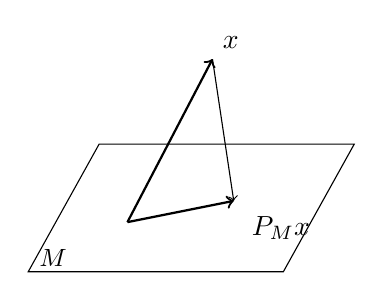
\begin{tikzpicture}[scale=0.9,baseline=(current bounding box.center)]
  \draw (0,0) -- (3.6,0) -- (4.6,1.8) -- (1,1.8) -- cycle;
  \node at (0.35,0.2) {\small $M$};
  \coordinate (O) at (1.4,0.7);
  \coordinate (P) at (2.9,1.0);
  \coordinate (X) at (2.6,3.0);
  \draw[->,thick] (O) -- (X) node[above right] {$x$};
  \draw[->,thick] (O) -- (P);
  \node[below right,xshift=3pt,yshift=-2pt] at (P) {$P_M x$};
  \draw[->] (X) -- (P);
\end{tikzpicture}
\qquad\qquad
$\begin{aligned}
&P_M\cdot P_M x = P_M x\\
&\underline{P_M^2 x = P_M x}
\end{aligned}$
\end{center}

\begin{remark}
An \term{orthogonal projection matrix} $P\in\C^{n\times n}$ satisfies
\begin{enumerate}[label=\roman*-), nosep]
  \item $P\Hm = P$
  \item $P^2 = P$ \quad ($P^k = P$ for every $k\ge 1$)
\end{enumerate}
Also,
\begin{align*}
(I-P)^2 &= I-P\\
(I-P)(I-P) &= I-\cancel{P}-P+\overbrace{P^2}^{\cancel{P}}\\
&= I-P
\end{align*}
\end{remark}
\begin{insight}[Remarks on $P_M$]
\begin{itemize}[nosep]
  \item Conversely, \key{any $P$ with $P\Hm=P$ and $P^2=P$ is the orthogonal projection onto $\Range(P)$}:
        $x = Px + (I-P)x$ with $Px\in\Range(P)$, and $(I-P)x\perp\Range(P)$ because
        \[
        (Py)\Hm(I-P)x = y\Hm(P-P^2)x = 0 \qquad\text{for all } y.
        \]
  \item \key{$P_M$ depends only on $M$}, not on the chosen basis: if $B' = BT$ with $T$ invertible, then
        $B'(B'^H B')^{-1}B'^H = BT\,T^{-1}(B\Hm B)^{-1}T^{-H}\,T\Hm B\Hm = P_M$.
  \item If the columns of $B$ are orthonormal, $B\Hm B = I$ and $P_M = BB\Hm = \sum_i m_i m_i\Hm$,
        which is the matrix form of $m^* = \sum_i\inner{x}{m_i}m_i$.
  \item $P_M m = m$ for $m\in M$ and $P_M y = 0$ for $y\in M^\perp$ (since $B\Hm y = 0$);
        hence $\Range(P_M) = M$, $\Null(P_M) = M^\perp$.
\end{itemize}
\end{insight}

% ===== Page 42 =====
\begin{example}
$\V=\R^3$,\origpage{42} \quad $M = \Span\left\{\bmat{1\\1\\1},\bmat{1\\-1\\1}\right\}$, \quad
$x = \bmat{1\\0\\0}$. \quad Find $\operatorname{Proj}_M x = \,?$
\begin{gather*}
B = \bmat{1&1\\1&-1\\1&1}, \qquad
B\Hm B = B\T B = \bmat{1&1&1\\1&-1&1}\bmat{1&1\\1&-1\\1&1} = \bmat{3&1\\1&3},\\[4pt]
(B\Hm B)^{-1} = \bmat{3&-1\\-1&3}\cdot\frac18
\end{gather*}
Then
\begin{align*}
\operatorname{Proj}_M x &= B(B\Hm B)^{-1}B\Hm x = P_M x\\
&= \frac18\bmat{1&1\\1&-1\\1&1}\bmat{3&-1\\-1&3}\underbrace{\bmat{1&1&1\\1&-1&1}\bmat{1\\0\\0}}_{\bmat{1\\1}}\\
&= \frac18\bmat{1&1\\1&-1\\1&1}\underbrace{\bmat{3&-1\\-1&3}\bmat{1\\1}}_{\bmat{2\\2}}\\
&= \frac18\cdot\bmat{4\\0\\4} = \bmat{1/2\\0\\1/2}\\[4pt]
x-\operatorname{Proj}_M x &= \bmat{1\\0\\0} - \bmat{1/2\\0\\1/2} = \bmat{1/2\\0\\-1/2}
\end{align*}
% note: in the notes the three products are shown as nested underbraces under one line
\explain{This difference should be orthogonal to the basis vectors (``sağlaması için kullanılabilir'' --- can be used to check the result).}
% Turkish: "can be used to verify (the result)"
\explain{Check, and the full projection matrix (its first column is indeed $\operatorname{Proj}_M x$):}
\begin{gather*}
\bmat{1&1&1}\bmat{1/2\\0\\-1/2} = 0, \qquad \bmat{1&-1&1}\bmat{1/2\\0\\-1/2} = 0 \quad\checkmark\\*[4pt]
P_M = \frac18 B\bmat{3&-1\\-1&3}B\T = \frac12\bmat{1&0&1\\0&2&0\\1&0&1}
\end{gather*}
\end{example}

% Section 6: Systems of Linear Equations $Ax=b$  (original handwritten pages 43--51)
\section{Systems of Linear Equations $Ax=b$}\label{sec:axb}
\syllabusweek{Week 7 --- systems of linear equations of the form $Ax=b$}
\subsection{Existence and Uniqueness of Solutions}\label{ss:exist-unique}
\[
Ax = b, \qquad A\in\C^{m\times n}, \quad x\in\C^n, \quad b\in\C^m
\]
\begin{center}
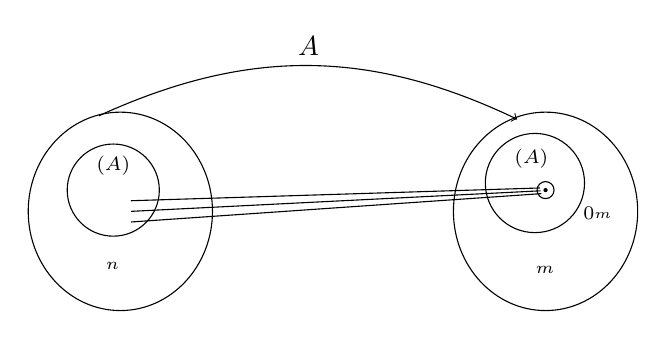
\begin{tikzpicture}[scale=0.9]
  % domain C^n
  \draw (0,0) ellipse (1.3 and 1.4);
  \draw (-0.1,0.3) circle (0.65);
  \node at (-0.1,0.65) {\scriptsize $\Null(A)$};
  \node at (-0.1,-0.85) {\small $\C^n$};
  % codomain C^m
  \draw (6,0) ellipse (1.3 and 1.4);
  \draw (5.85,0.4) circle (0.7);
  \node at (5.8,0.75) {\scriptsize $\Range(A)$};
  \draw (6.0,0.3) circle (0.12);
  \fill (6.0,0.3) circle (0.03);
  \node at (6.75,-0.05) {\scriptsize $0_{\C^m}$};
  % corrected: second small "C^m" label next to the zero vector; read as the subscript of 0 (0_{C^m}), consistent with N(A)={x: Ax=0_{C^m}}
  \node at (6,-0.9) {\small $\C^m$};
  % map
  \draw[->] (-0.3,1.35) to[bend left=25] node[above] {$A$} (5.6,1.3);
  \draw (0.15,0.15) -- (5.92,0.33);
  \draw (0.15,0.0) -- (5.93,0.29);
  \draw (0.15,-0.15) -- (5.94,0.25);
\end{tikzpicture}
\end{center}
\explain{$A$ maps every vector of $\Null(A)$ to $0_{\C^m}$.}
The two fundamental subspaces of $A$:
\begin{align*}
\text{\term{range space}: }\Range(A) &= \{y\in\C^m \mid \exists x\in\C^n \text{ satisfying } y=Ax\}\\
\text{\term{null space}: }\Null(A) &= \{x\in\C^n \mid Ax = 0_{\C^m}\}
\end{align*}
Rank--nullity:
\begin{gather*}
\underbrace{\dim(\Range(A))}_{\text{rank}} + \underbrace{\dim(\Null(A))}_{\text{nullity}} = n = \#\text{ of columns of } A
\end{gather*}
Recall also, for a subspace $M$ of $\V$:
\begin{align*}
&\V = M\overset{\perp}{\oplus}M^\perp\\
&v = v_1+v_2, \qquad v_1\in M, \quad v_2\in M^\perp, \qquad v_1,v_2 \text{ are unique}\\
&v_1\perp v_2, \qquad \dim M + \dim M^\perp = \dim \V
\end{align*}
Two questions:
\begin{enumerate}[label=\arabic*-), nosep]
  \item Is there an exact solution? \ ($\Range(A)$)
  \item If there is, is it unique? \ ($\Null(A)$)
\end{enumerate}
\explain{Question 1 is answered by $\Range(A)\subseteq\C^m$ (the codomain side), question 2 by $\Null(A)\subseteq\C^n$ (the domain side).}

% ===== Page 43 =====
\sep
\point $\displaystyle \underbrace{\bmat{1\\1}}_{A}\underset{\in\R}{x} = \underbrace{\bmat{2\\2}}_{b}$,
\qquad $b\in\Range(A)$\origpage{43}\\[4pt]
$\Rightarrow$ $\exists$ an exact solution. \quad $\Rightarrow$ The solution is unique.

\point $\displaystyle \underbrace{\bmat{1\\1}}_{A}x = \underbrace{\bmat{2\\1}}_{b}$
\quad $\Rightarrow$ No exact solution! \qquad $b\notin\Range(A)$
\begin{align*}
y = Ax &= \big[\,a_1 \,\vdots\, a_2 \,\vdots\, a_3 \,\vdots\, \cdots \,\vdots\, a_n\,\big]\bmat{x_1\\x_2\\ \vdots\\ x_n}
= x_1\vec a_1 + x_2\vec a_2 + \dots + x_n\vec a_n\\[4pt]
\Range(A) &= \Span\{\vec a_1,\vec a_2,\dots,\vec a_n\} \triangleq \text{\term{column space} of } A\\
\Range(A) &= \Span\left\{\bmat{1\\1}\right\}, \qquad \bmat{2\\1}\notin\Range(A)
\end{align*}

\begin{keybox}
$\therefore$ 1-) \key{There exists an exact solution iff $b\in\Range(A)$.}
\end{keybox}

\point $\displaystyle \underbrace{\bmat{1&2\\1&2}}_{A}\underset{\in\R^2}{x} = \underbrace{\bmat{2\\2}}_{b}$:
\quad $\Range(A) = \Span\left\{\bmat{1\\1}\right\}$ \& $b\in\Range(A)$ $\Rightarrow$ $\therefore\ \exists$ an exact solution
\[
x_1 = \bmat{2\\0} \quad\text{or}\quad x_2 = \bmat{0\\1} \quad\text{or}\quad x_3 = \bmat{4\\-1} \quad\dots
\]

\needspace{14\baselineskip}
\sep
Dimensions in the first example:
\begin{gather*}
\left.\begin{aligned}
A &= \bmat{1\\1}, \qquad \dim\C = 1\\
\Range(A) &= \Span\left\{\bmat{1\\1}\right\}, \qquad \dim\Range(A) = 1
\end{aligned}\right\}
\quad
\begin{aligned}
&\underbrace{\dim(\Range(A))}_{1} + \underbrace{\dim(\Null(A))}_{0} = 1 \leftarrow \#\text{ of columns}\\
&\Null(A) = \{0\}, \qquad \dim(\Null(A)) = 0
\end{aligned}
\end{gather*}
and in the third example:
\begin{align*}
&A = \bmat{1&2\\1&2}, \qquad \Range(A) = \Span\left\{\bmat{1\\1}\right\}, \qquad \dim\Range(A) = 1\\
&\underbrace{\dim\Range(A)}_{1} + \underbrace{\dim\Null(A)}_{1} = 2, \qquad
\Null(A) = \Span\left\{\bmat{2\\-1}\right\}\\[4pt]
&x_1-x_2 = \bmat{2\\-1}, \qquad x_1-x_3 = \bmat{-2\\1}, \qquad x_2-x_3 = \bmat{-4\\2} \qquad \text{all inside null space.}
\end{align*}

\needspace{10\baselineskip}
\sep
In general:
\begin{align*}
&A\hat x = b \qquad \hat x \text{ is exact}\\
&\underset{\substack{\uparrow\\ \in\Null(A)}}{\hat x + m} \;\Rightarrow\; A(\hat x+m) = A\hat x + \underbrace{\overset{\in\Null(A)}{Am}}_{0} = b+0 = b
\end{align*}
% corrected: notes had "= b+0 = 0" at the end (meant "= b") and "x is exact" (meant \hat x)
\begin{itemize}[nosep]
  \item if $\hat x$ satisfies $A\hat x = b$ exactly $\Rightarrow$ $\hat x + m$ satisfies $A(\hat x+m) = b$ exactly \ ($m\in\Null(A)$);
  \item if $m\neq 0 \Rightarrow \hat x \neq \hat x + m$;
  \item if $\Null(A)$ includes nonzero vectors $\Rightarrow$ \key{infinitely many exact solutions}.
\end{itemize}

% ===== Page 44 =====
\origpage{44}
\begin{keybox}
$\therefore$ 2-) If an exact solution $\hat x$ exists, then \key{it is unique
$\iff \Null(A) = \{0\}$} \ or \ $\dim\Null(A) = 0$.
\end{keybox}
\needspace{7\baselineskip}
\begin{insight}
Conversely, if $A\hat x = b$ and $A\tilde x = b$, then $A(\hat x-\tilde x) = 0$, i.e.\ any two exact solutions
differ by a vector of $\Null(A)$. Hence \key{the full solution set is the affine set
$\{\hat x + m : m\in\Null(A)\}$}. By rank--nullity, $\Null(A)=\{0\}$ iff $\rank A = n$ (the columns of $A$ are
linearly independent); this requires $m\ge n$.
\end{insight}

\subsection{Least-Squares Solutions}\label{ss:least-squares}
\point $\displaystyle \bmat{1\\1}x = \bmat{2\\1}$, \qquad $Ax = b$, \qquad $b\notin\Range(A)$

\paragraph{\term{Least-squares problem}.}
\[
\min_{x\in\C^n} \underbrace{\norm{Ax-b}^{2}}_{\text{error}}
\]
\explain{The exponent $2$ doesn't matter; $\norm{\cdot}$ is the induced norm of the inner product.}
\[
\hat x = \arg\min_{x\in\C^n}\norm{Ax-b}
\]
\explain{$\hat x$: \term{minimum error solution} / \term{least-squares solution}.}
Since $b\in\C^m$, decompose it:
\begin{align*}
\C^m &= M\overset{\perp}{\oplus}M^\perp\\
\C^m &= \Range(A)\overset{\perp}{\oplus}\Range^\perp(A)\\
b &= \underset{\in\Range(A)}{b_1} + \underset{\in\Range^\perp(A)}{b_2}
\;\Rightarrow\; b_1 = \operatorname{Proj}_{\Range(A)} b, \quad b_2 = \operatorname{Proj}_{\Range^\perp(A)} b
\;\Rightarrow\; b_1\perp b_2
\end{align*}
\needspace{15\baselineskip}
Then
\begin{align*}
\norm{Ax-b}^2 &= \inner{Ax-b}{Ax-b}\\
&= \big\langle (\underset{\in\Range(A)}{Ax}-\underset{\in\Range(A)}{b_1}) - \underset{\in\Range^\perp(A)}{b_2},\ (Ax-b_1)-b_2\big\rangle
&& (\Range(A) \text{ is a subspace})\\
&= \inner{Ax-b_1}{Ax-b_1}\\
&\quad \cancel{-\inner{Ax-b_1}{b_2}}\\
&\quad \cancel{-\inner{b_2}{Ax-b_1}} && (\to 0 \text{ because of orthogonality})\\
&\quad +\inner{b_2}{b_2}\\
&= \inner{Ax-b_1}{Ax-b_1} + \inner{b_2}{b_2}\\
&= \overbrace{\Big\lVert A\underset{\substack{\uparrow\\ \text{find an } x}}{x}-\underset{\in\Range(A)}{b_1}\Big\rVert^2}^{\text{zero}} + \norm{b_2}^2 \geq \norm{b_2}^2
\end{align*}
% corrected: notes had the first term without the square, i.e. ||Ax-b_1|| + ||b_2||^2
\explain{\key{The first term can be made zero}: $b_1\in\Range(A)$, so some $x$ satisfies $Ax=b_1$ exactly.}
\needspace{8\baselineskip}
Therefore
\begin{gather*}
\boxed{\min_{x\in\C^n}\norm{Ax-b} = \norm{b_2} = \norm{\operatorname{Proj}_{\Range^\perp(A)} b}}\\*[4pt]
A\hat x = b_1, \qquad \hat x = \arg\min_{x\in\C^n}\norm{Ax-b}, \qquad
b_1 = \operatorname{Proj}_{\Range(A)} b\\*[4pt]
\underbrace{\hat x}_{\substack{\text{min error /}\\ \text{least-squares solution}}} = \arg\min_{x\in\C^n}\norm{Ax-b}
\end{gather*}
\begin{insight}[Normal equations]
$A\hat x = b_1$ is equivalent to $b - A\hat x = b_2 \perp \Range(A)$, i.e.\ $a_j\Hm(b-A\hat x) = 0$ for every
column $a_j$ of $A$:
\[
A\Hm(b-A\hat x) = 0 \quad\Longleftrightarrow\quad \boxed{A\Hm A\,\hat x = A\Hm b}
\]
(the same equations as $B\Hm B\alpha^* = B\Hm x$ before, with $B=A$). \key{These normal equations always have a
solution.} If the columns of $A$ are linearly independent, $A\Hm A$ is invertible and
$\hat x = (A\Hm A)^{-1}A\Hm b$ is unique; otherwise there are infinitely many least-squares solutions,
differing by elements of $\Null(A\Hm A)=\Null(A)$.
\end{insight}

% ===== Page 45 =====
\sep
\point $\displaystyle \bmat{1\\1}x = \bmat{2\\1}$, \qquad $b\notin\Range(A)$, \qquad
$\Range(A) = \Span\left\{\bmat{1\\1}\right\}$\origpage{45}
\begin{align*}
&P_{\Range(A)} = B(B\Hm B)^{-1}B\Hm, \qquad B = \bmat{1\\1}, \qquad B\Hm B = \bmat{1&1}\bmat{1\\1} = 2\\
&P_{\Range(A)} = \bmat{1\\1}\frac12\bmat{1&1} = \bmat{1/2&1/2\\1/2&1/2}\\
&b_1 = P_{\Range(A)}b = \bmat{1/2&1/2\\1/2&1/2}\bmat{2\\1} = \bmat{3/2\\3/2}\\
&\underbrace{\bmat{1\\1}}_{A}\hat x = \underbrace{\bmat{3/2\\3/2}}_{b_1},
\qquad \hat x = \frac32
\end{align*}
\explain{$\hat x = \tfrac32$ is the average of the entries of $b = \bmat{2 & 1}\T$.}
\explain{Same result from the normal equations: $A\Hm A = 2$, $A\Hm b = 3$ $\Rightarrow$ $\hat x = \tfrac32$; $b-b_1 = \bmat{1/2 & -1/2}\T$, so the minimum error is $\norm{b-b_1} = \tfrac1{\sqrt2}$.}

\point $\displaystyle \bmat{1\\1}x = \bmat{2\\1}$, \qquad
$\Range(A) = \Span\left\{\bmat{1\\1}\right\}$
\[
b_1 = P_{\Range(A)}b = \bmat{1/2&1/2\\1/2&1/2}\bmat{2\\1} = \bmat{3/2\\3/2}
\]
% corrected: notes had the multiplied vector as [1;1] (it is b=[2;1])
Then
\begin{alignat*}{2}
&A\hat x = b_1, &\qquad& \hat x = 3/2\\
&\Null(A) = \{0\},\ \dim\Null(A) = 0 &\qquad& \Rightarrow\ \hat x \text{ \key{is unique.}}
\end{alignat*}

\point $\displaystyle \bmat{1&2\\1&2}x = \bmat{2\\1}$, \qquad
$\Range(A) = \Span\left\{\bmat{1\\1}\right\}$, \qquad $b\notin\Range(A)$
\begin{align*}
&b_1 = P_{\Range(A)}b = \bmat{3/2\\3/2}\\
&\bmat{1&2\\1&2}\hat x = \bmat{3/2\\3/2}
\quad\Rightarrow\quad \hat x = \bmat{3/2\\0}, \quad \hat x = \bmat{0\\3/4}, \quad \hat x = \bmat{1/2\\1/2}\\
&\Null(A) = \Span\left\{\bmat{2\\-1}\right\}
\quad\Rightarrow\quad \hat x \text{ \key{is not unique!}}
\end{align*}
\explain{All least-squares solutions: $\hat x = \bmat{3/2 & 0}\T + t\bmat{2 & -1}\T$, $t\in\R$ (e.g.\ $t=-\tfrac34$ gives $\bmat{0 & 3/4}\T$, $t=-\tfrac12$ gives $\bmat{1/2 & 1/2}\T$). Each leaves the same error $\norm{b_2} = \tfrac1{\sqrt2}$.}

\subsection{Minimum-Norm Solutions}\label{ss:min-norm}
\paragraph{\term{Minimum-norm solution}.}
\begin{gather*}
b\in\Range(A) \;\Rightarrow\; \min_{Ax=b}\norm{x}, \qquad
\hat x_1 = \arg\min_{Ax=b}\norm{x}, \qquad x = \hat x + \overset{\in\Null(A)}{m}\\[4pt]
\min_{m\in\Null(A)}\norm{\hat x + m}, \qquad A\hat x = b
\end{gather*}
\explain{When there are infinitely many solutions, pick the one with the smallest norm. Every solution has the form $\hat x+m$ for one fixed solution $\hat x$, so we minimize over $m\in\Null(A)$.}
\begin{center}
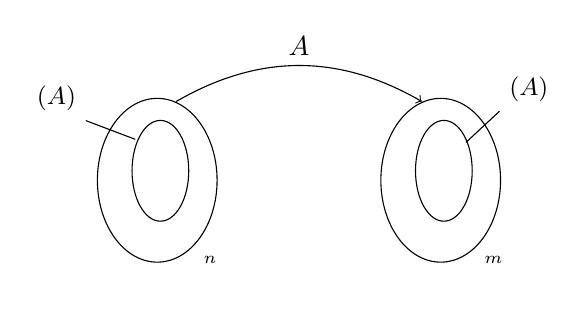
\begin{tikzpicture}[scale=0.8]
  \draw (0,0) ellipse (0.95 and 1.3);
  \draw (0.05,0.15) ellipse (0.45 and 0.8);
  \node at (0.85,-1.35) {\small $\C^n$};
  \node (NA) at (-1.6,1.3) {\small $\Null(A)$};
  \draw (-0.35,0.65) -- (NA.south east);
  \draw (4.5,0) ellipse (0.95 and 1.3);
  \draw (4.55,0.15) ellipse (0.45 and 0.8);
  \node at (5.35,-1.35) {\small $\C^m$};
  \node (RA) at (5.9,1.45) {\small $\Range(A)$};
  \draw (4.9,0.6) -- (RA.south west);
  \draw[->] (0.3,1.25) to[bend left=30] node[above] {$A$} (4.2,1.25);
\end{tikzpicture}
\end{center}
\begin{align*}
&\C^m = \Range(A)\overset{\perp}{\oplus}\Range^\perp(A)\\
&\C^n = \Null^\perp(A)\overset{\perp}{\oplus}\Null(A)\\
&\hat x = \underset{\in\Null^\perp(A)}{\hat x_1} + \underset{\in\Null(A)}{\hat x_2},
\qquad \hat x_1 = \operatorname{Proj}_{\Null^\perp(A)}\hat x, \quad \hat x_2 = \operatorname{Proj}_{\Null(A)}\hat x,
\qquad \hat x_1\perp\hat x_2
\end{align*}

% ===== Page 46 =====
Then\origpage{46}
\begin{align*}
\norm{\hat x + m}^2 &= \inner{\hat x + m}{\hat x + m}\\
&= \big\langle \underset{\in\Null^\perp}{\hat x_1} + (\underset{\in\Null}{\hat x_2} + \underset{\in\Null}{m}),\ \underset{\in\Null^\perp}{\hat x_1} + (\underset{\in\Null}{\hat x_2} + \underset{\in\Null}{m})\big\rangle\\
&= \inner{\hat x_1}{\hat x_1} + \inner{\hat x_2 + m}{\hat x_2 + m}\\
&= \norm{\hat x_1}^2 + \norm{\hat x_2 + m}^2\\
&\geq \norm{\hat x_1}^2
\end{align*}
\explain{Equality for $m^* = -\hat x_2 \;\Rightarrow\; \norm{\hat x_2 + m} = 0$.}
Hence
\begin{gather*}
\min_{\substack{Ax=b\\ m\in\Null(A)}} \norm{\hat x + m} = \norm{\hat x - \hat x_2} = \norm{\hat x_1}
\end{gather*}
and $\hat x_1$ is itself a solution:
\begin{align*}
A\hat x &= b\\
A(\hat x_1 + \hat x_2) &= b\\
A\hat x_1 + \underbrace{\cancel{A\hat x_2}}_{0} &= b\\
\Rightarrow\quad A\hat x_1 &= b\\[4pt]
&\boxed{\hat x_1 = \operatorname{Proj}_{\Null^\perp(A)}\hat x = \text{minimum-norm solution}}
\end{align*}
\begin{insight}[Summary of the method]
\begin{itemize}[nosep]
  \item $\hat x_1$ does not depend on which solution $\hat x$ we start from: two solutions differ by an element
        of $\Null(A)$, which the projection onto $\Null^\perp(A)$ removes. So \key{the minimum-norm solution is unique}.
  \item $\Null^\perp(A) = \Range(A\Hm)$ (since $Ax=0 \iff x\perp$ every row of $A$, i.e.\ every column of $A\Hm$).
        Hence the minimum-norm solution can be written $\hat x_1 = A\Hm z$, and $AA\Hm z = b$; if $A$ has
        linearly independent rows, $\hat x_1 = A\Hm(AA\Hm)^{-1}b$.
  \item If $b\notin\Range(A)$, combine both steps: replace $b$ by $b_1 = \operatorname{Proj}_{\Range(A)}b$, take any
        least-squares solution and project it onto $\Null^\perp(A)$. The result is the \term{minimum-norm
        least-squares solution} (this is what the pseudo-inverse $A^{+}b$ computes); the example below does exactly this.
\end{itemize}
\end{insight}

\begin{example}
\begin{gather*}
\bmat{1&2\\1&2}x = \bmat{2\\1}, \qquad
b_1 = \operatorname{Proj}_{\Range(A)} b = \bmat{3/2\\3/2}\\[4pt]
\bmat{1&2\\1&2}\hat x = \bmat{3/2\\3/2}
\quad\Rightarrow\quad
\hat x = \bmat{3/2\\0}\\[4pt]
\Null(A) = \Span\left\{\bmat{2\\-1}\right\}, \qquad
\underbrace{\dim\Null(A)}_{1} + \underbrace{\dim\Null^\perp(A)}_{1} = 2\\[4pt]
\Null^\perp(A) = \Span\Big\{\underbrace{\bmat{1\\2}}_{v}\Big\} = \Range(A\Hm)\\[4pt]
P_{\Null^\perp(A)} = B(B\Hm B)^{-1}B\Hm \;\overset{B=v}{=}\; \frac{vv\Hm}{v\Hm v}
= \frac{\bmat{1\\2}\bmat{1&2}}{\bmat{1&2}\bmat{1\\2}} = \frac15\bmat{1&2\\2&4}\\[4pt]
\hat x_1 = \frac15\bmat{1&2\\2&4}\bmat{3/2\\0} = \frac15\bmat{3/2\\3} = \bmat{3/10\\3/5}
\end{gather*}
\begin{insight}[Checking the answer]
\begin{itemize}[nosep]
  \item $A\hat x_1 = \bmat{3/10+6/5\\ 3/10+6/5} = \bmat{3/2\\3/2} = b_1$, so $\hat x_1$ is a least-squares solution.
  \item $\hat x_1 = \tfrac{3}{10}\bmat{1 & 2}\T\in\Null^\perp(A)$, i.e.\ $\hat x_1\perp\bmat{2 & -1}\T$.
  \item Starting from $\bmat{0 & 3/4}\T$ or $\bmat{1/2 & 1/2}\T$ instead gives the same $\hat x_1$, e.g.
        \[
        \tfrac15\bmat{1&2\\2&4}\bmat{0\\3/4} = \bmat{3/10\\3/5}.
        \]
  \item Norms: $\norm{\hat x_1}^2 = \tfrac{9}{20} = 0.45$, smaller than
        $\norm{\bmat{3/2 & 0}\T}^2 = 2.25$, $\norm{\bmat{0 & 3/4}\T}^2 = 0.5625$ and $\norm{\bmat{1/2 & 1/2}\T}^2 = 0.5$.
\end{itemize}
\end{insight}
\end{example}

% ===== Page 47 =====
\subsection{General Procedure and the Fundamental Theorem}\label{ss:procedure}
\begin{itemize}[leftmargin=1.5em,topsep=0pt]
\item If $b\in\Range(A)$:\origpage{47} \key{$\exists$ an exact solution} to $A\hat{x}=b$.
\item If $b\notin\Range(A)$:
\[
b_1=\operatorname{Proj}_{\Range(A)} b, \qquad A\hat{x}=b_1
\]
\begin{itemize}
\item If $\Null(A)=\{0\}$ $\Rightarrow$ \key{$\hat{x}$ is unique}.
\item If $\Null(A)\neq\{0\}$ $\Rightarrow$ $\hat{x}_1=\operatorname{Proj}_{\Null^\perp(A)}\hat{x}$.
\end{itemize}
\end{itemize}

\begin{center}
\begin{tabular}{@{}l@{\quad}l@{}}
$\hat{x}$: & \term{minimum error solution} (least-squares)\\
$\hat{x}_1$: & \term{minimum error-norm solution}
\end{tabular}
\end{center}

\begin{insight}[Why the procedure works]
\begin{itemize}[nosep,leftmargin=1.2em]
\item The error $b-A\hat x$ is smallest when $A\hat x$ is the point of $\Range(A)$ closest to $b$, i.e.\ $A\hat x=b_1=\operatorname{Proj}_{\Range(A)}b$ (orthogonality principle: $b-b_1\perp\Range(A)$). Writing this as $A\Hm(b-A\hat x)=0$ gives the \term{normal equations} $A\Hm A\hat x=A\Hm b$.
\item If $\Null(A)\neq\{0\}$, every $\hat x+n$ with $n\in\Null(A)$ gives the same $A\hat x=b_1$, so the least-squares solution is not unique. Splitting $\hat x=\hat x_1+\hat x_2$ with $\hat x_1\in\Null^\perp(A)$, $\hat x_2\in\Null(A)$ gives $A\hat x_1=A\hat x=b_1$ and, by Pythagoras, $\norm{\hat x+n}^2=\norm{\hat x_1}^2+\norm{\hat x_2+n}^2\geq\norm{\hat x_1}^2$. Hence \key{$\hat x_1$ is the least-squares solution of minimum-norm}, and it does not depend on which $\hat x$ we started from.
\end{itemize}
\end{insight}

\begin{example}
$A=\bmat{1&2&3\\1&2&3}$, \qquad $n=3$, $m=2$ \quad ($A\in\C^{m\times n}$: $n$ columns, $m$ rows).
\begin{align*}
\Range(A)&=\Span\left\{\bmat{1\\1}\right\}, \qquad \dim(\Range(A))=1\\
\Null(A)&=\Span\left\{\bmat{3\\0\\-1},\bmat{2\\-1\\0}\right\}
\end{align*}
\[
\underbrace{\dim(\Range(A))}_{1}+\underbrace{\dim(\Null(A))}_{2}=3,
\qquad
\underbrace{\dim(\Null(A))}_{2}+\underbrace{\dim(\Null^\perp(A))}_{1}=3
\]
For $\Null^\perp(A)$, a vector $[a\ b\ c]\T$ orthogonal to both basis vectors of $\Null(A)$:
\[
\begin{aligned}3a-c&=0\\2a-b&=0\end{aligned}
\quad\Rightarrow\quad
\begin{aligned}c&=3a\\b&=2a\end{aligned}
\quad\Rightarrow\quad \bmat{a\\b\\c}=a\underbrace{\bmat{1\\2\\3}}_{\text{row of }A}
\qquad\Rightarrow\qquad
\Null^\perp(A)=\Span\left\{\bmat{1\\2\\3}\right\}
\]
\[
\Null^\perp(A)=\Range(A\Hm)
\]
\explain{$\therefore$ \key{Fundamental theorem of linear algebra.}}
\[
\hat{x}_1=\operatorname{Proj}_{\Null^\perp(A)}\hat{x}
=\operatorname{Proj}_{\Range(A\Hm)}\hat{x}
\]
\explain{$\Range(A\Hm)$: row space of $A$.}
\end{example}

\paragraph{Dimensions and rank.} For $A\in\C^{m\times n}$:
\begin{align*}
\dim(\underbrace{\Range(A)}_{k})+\dim(\underbrace{\Null(A)}_{n-k}) &= \#\text{ of columns}=n\\
\dim(\underbrace{\Null(A)}_{n-k})+\dim(\underbrace{\Range(A\Hm)}_{k})&=n
\qquad \big(\dim(\Null(A))+\dim(\Null^\perp(A))=n\big)
\end{align*}
\[
\left.\begin{aligned}
\dim(\Range(A))&=\#\text{ of lin.\ indep.\ columns of }A=\text{column rank}=k\\
\dim(\Range(A\Hm))&=\#\text{ of lin.\ indep.\ rows of }A=\text{row rank}=k
\end{aligned}\right\}\ k=\text{\term{rank} of a matrix}
\]
\[
\#\text{ linearly indep.\ rows}=\#\text{ linearly indep.\ columns}
\quad\text{as}\quad \dim\Range(A)=k=\dim\Range(A\Hm)
\]
$k$: \key{\# of linearly independent rows $=$ \# of linearly independent columns} (column rank $=$ row rank).

% ===== Page 48 =====
\begin{theorem}[Fundamental theorem of linear algebra]\leavevmode\origpage{48}
$\Range(A\Hm)=\Null^\perp(A)$
\end{theorem}
\begin{proof}
$\inner{x}{y}\triangleq y\Hm x$.
\[
\inner{\underset{\C^m}{Ax}}{\underset{\C^m}{y}}_{\C^m}=y\Hm Ax=(A\Hm y)\Hm x=\inner{\underset{\C^n}{x}}{\underset{\C^n}{A\Hm y}}_{\C^n}
\]
Prove $\Null(A)=\Range^\perp(A\Hm)$, which is easier to prove.
\[
\left.\begin{aligned}
\Null(A)&\subset\Range^\perp(A\Hm)\\
\Range^\perp(A\Hm)&\subset\Null(A)
\end{aligned}\right\}\ \text{prove both}\ \Rightarrow\ \Null(A)=\Range^\perp(A\Hm)
\]

\paragraph{Part 1.} $x\in\Null(A)\Rightarrow Ax=0$.

\begin{minipage}{0.25\textwidth}
\centering
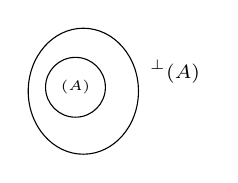
\begin{tikzpicture}
\draw (0,0) ellipse (0.7 and 0.8);
\draw (-0.1,0.05) circle (0.38);
\node[font=\tiny] at (-0.1,0.05) {$\Null(A)$};
\node[font=\scriptsize,anchor=west] at (0.72,0.25) {$\Range^\perp(A\Hm)$};
\end{tikzpicture}
\end{minipage}\hfill
\begin{minipage}{0.72\textwidth}
\begin{align*}
&\inner{Ax}{y}\quad\text{where }\forall y\in\C^m\\
&\inner{Ax}{y}=0\\
&\inner{x}{A\Hm y}=0\quad\forall y\in\C^m\\
\Rightarrow\ & x\perp A\Hm y\quad\forall y\in\C^m\\
\Rightarrow\ & x\perp\Range(A\Hm)\Rightarrow x\in\Range^\perp(A\Hm)
\end{align*}
\end{minipage}

\paragraph{Part 2.} $x\in\Range^\perp(A\Hm)$.

\begin{minipage}{0.25\textwidth}
\centering
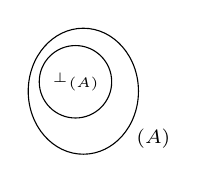
\begin{tikzpicture}
\draw (0,0) ellipse (0.7 and 0.8);
\draw (-0.1,0.12) circle (0.46);
\node[font=\tiny] at (-0.1,0.12) {$\Range^\perp(A\Hm)$};
\node[font=\scriptsize,anchor=west] at (0.55,-0.6) {$\Null(A)$};
\end{tikzpicture}
\end{minipage}\hfill
\begin{minipage}{0.72\textwidth}
\begin{align*}
&x\in\Range^\perp(A\Hm)\\
\Rightarrow\ & x\perp A\Hm y\quad\forall y\in\C^m\\
&\inner{x}{A\Hm y}=0\quad\forall y\in\C^m\\
&\inner{Ax}{y}=0\quad\forall y\in\C^m
\end{align*}
\explain{$Ax\in\C^m$, so choose $y=Ax$:}
\[
\inner{Ax}{Ax}=\norm{Ax}^2=0\Rightarrow Ax=0\Rightarrow x\in\Null(A)
\]
\end{minipage}

Both inclusions hold, so $\Null(A)=\Range^\perp(A\Hm)$. Taking orthogonal complements of both sides (in finite dimensions $(S^\perp)^\perp=S$ for a subspace $S$) gives $\Null^\perp(A)=\Range(A\Hm)$.
\end{proof}

\begin{center}
\begin{minipage}{0.46\textwidth}
\centering
\begin{tikzpicture}[scale=0.85]
\draw (0,0) ellipse (1.1 and 1.25);
\draw (0.05,0.15) ellipse (0.6 and 0.8);
\node[font=\scriptsize] at (0.05,-0.85) {$\Null(A)$};
\node at (0.9,-1.45) {$\C^n$};
\draw (3.8,0) ellipse (1.0 and 1.25);
\draw (3.75,0.15) ellipse (0.6 and 0.8);
\node[font=\scriptsize] at (3.75,-0.85) {$\Range(A)$};
\node at (4.75,-1.45) {$\C^m$};
\fill (3.55,0.45) circle (1.2pt) node[right,font=\scriptsize]{$0$};
\draw[-{Stealth[length=1.5mm]}] (-0.3,0.55) to[bend left=6] (3.5,0.47);
\draw[-{Stealth[length=1.5mm]}] (-0.25,0.25) to[bend left=3] (3.5,0.45);
\draw[-{Stealth[length=1.5mm]}] (-0.2,0.0) to[bend right=4] (3.5,0.43);
\draw[-{Stealth[length=2mm]}] (0.3,1.5) to[bend left=15] node[above]{$A$} (3.4,1.45);
\end{tikzpicture}
\end{minipage}\hfill
\begin{minipage}{0.5\textwidth}
\begin{align*}
&\dim(\overset{k}{\Range(A)})+\dim(\overset{n-k}{\Null(A)})=n\\
&\dim(\Null(A))+\dim(\Null^\perp(A))=n\\
&\underbrace{\dim(\Range(A\Hm))}_{k}+\underbrace{\dim(\Null(A))}_{n-k}=n\\
&\underbrace{\dim(\Range(A))}_{\text{column rank}}=\underbrace{\dim(\Range(A\Hm))}_{\text{row rank}}=k
\end{align*}
\explain{$k$: rank.}
\end{minipage}
\end{center}

\subsection{Special Cases by Rank}\label{ss:rank-cases}
\subsubsection{Case I: Full Column Rank}
$A$ is/has \term{full column rank}: columns of $A$ are linearly independent.
\[
m\Big\{\underbrace{\overset{n}{\bmat{\ &\ &\ \\ \ &\ &\ \\ \ &\ &\ }}}_{\text{tall matrix}}
\overset{n}{\bmat{\ \\ \ \\ \ }}=\bmat{\ \\ \ \\ \ }\Big\}m \qquad m\geq n
\]
\begin{itemize}[nosep,leftmargin=1.5em]
\item $n=\#$ of unknowns, \quad $m=\#$ of equations
\item $m>n$: \term{overdetermined} system of equations
\end{itemize}
Assume
\[
\bmat{a&b&c\\d&e&f}\qquad\text{3 vectors cannot be linearly indep.\ for }\R^2.
\]
\explain{Under the columns: ``2 dim'', ``2 dimension''. Each column lies in $\R^2$, so at most $2$ of them can be linearly independent; full column rank therefore forces $m\geq n$.}

% ===== Page 49 =====
\origpage{49}
\begin{align*}
&\dim(\Range(A))=n\\
&\dim(\Null(A))=0\Rightarrow \Null(A)=\{0\} \qquad A\text{ is one-to-one}
\end{align*}
\key{If we have an exact solution, then the solution is unique.}

If $b\notin\Range(A)$:
\begin{align*}
P_{\Range(A)}&=B(B\Hm B)^{-1}B\Hm\\
\intertext{with $B=A$:}
P_{\Range(A)}&=A(A\Hm A)^{-1}A\Hm\\
b_1=P_{\Range(A)}b&=A(A\Hm A)^{-1}A\Hm b \qquad (A\hat{x}=b_1)\\
\Rightarrow\quad A\big(\underbrace{\hat{x}-(A\Hm A)^{-1}A\Hm b}_{\in\Null(A)}\big)&=0\\
\Rightarrow\quad \hat{x}-(A\Hm A)^{-1}A\Hm b&=0
\ \Rightarrow\ \boxed{\hat{x}=(A\Hm A)^{-1}A\Hm b}
\end{align*}
\explain{Unique solution as $\Null(A)=\{0\}$.}
$(A\Hm A)^{-1}A\Hm$: \term{left pseudo inverse} of $A$.

\begin{insight}
\begin{itemize}[nosep,leftmargin=1.2em]
\item \key{$A\Hm A$ ($n\times n$) is invertible exactly when $A$ has full column rank}: $A\Hm Ax=0\Rightarrow x\Hm A\Hm Ax=\norm{Ax}^2=0\Rightarrow Ax=0\Rightarrow x=0$.
\item The same formula comes directly from the normal equations $A\Hm A\hat x=A\Hm b$.
\item ``Left'' inverse: $\big((A\Hm A)^{-1}A\Hm\big)A=I_n$. If $b\in\Range(A)$, it returns the exact solution.
\end{itemize}
\end{insight}

\subsubsection{Case II: Full Row Rank}
$A$ is/has \term{full row rank}: all rows of $A$ are linearly independent.
\[
m\Big\{\underbrace{\overset{n}{\bmat{\ &\ &\ &\ \\ \ &\ &\ &\ }}}_{\text{fat matrix}}
\bmat{\ \\ \ \\ \ \\ \ }=\bmat{\ \\ \ } \qquad m\leq n
\]
\begin{itemize}[nosep,leftmargin=1.5em]
\item $m$: \# of equations, \quad $n$: \# of unknowns
\item $m<n$: \term{underdetermined} system of equations
\end{itemize}
\begin{align*}
\dim(\Range(A\Hm))&=m\\
\dim(\Range(A))&=m \ \Rightarrow\ \Range(A)=\C^m
\end{align*}
\[
b\in\Range(A)\quad\forall b\in\C^m\Rightarrow\text{\key{Always has an exact solution} (at least one): $A$ is onto.}
% corrected: notes had "b in C^m  for all b in R(A)" (quantifiers swapped)
\]
\begin{align*}
\hat{x}_1&=\operatorname{Proj}_{\Null^\perp(A)}\hat{x}=\operatorname{Proj}_{\Range(A\Hm)}\hat{x}\\
% corrected: notes had Proj_{R(A^H)} x-hat = Proj_{R(A^H)} x-hat (first projection meant onto N^perp(A))
\intertext{with $B=A\Hm$:}
P_{\Range(A\Hm)}&=A\Hm(AA\Hm)^{-1}A\\
\hat{x}_1&=A\Hm(AA\Hm)^{-1}\underbrace{A\hat{x}}_{b}\ \Rightarrow\ \hat{x}_1=A\Hm(AA\Hm)^{-1}b
\end{align*}
$A\Hm(AA\Hm)^{-1}$: \term{right pseudo inverse} of $A$.

\begin{insight}
\begin{itemize}[nosep,leftmargin=1.2em]
\item $AA\Hm$ ($m\times m$) is invertible since the rows of $A$ are independent (same argument as for $A\Hm A$, applied to $A\Hm$).
\item ``Right'' inverse: $A\big(A\Hm(AA\Hm)^{-1}\big)=I_m$, so $A\hat x_1=b$ is indeed an exact solution.
\item $\hat x_1=A\Hm\big((AA\Hm)^{-1}b\big)\in\Range(A\Hm)=\Null^\perp(A)$, so \key{it is the minimum-norm one} among the infinitely many exact solutions $\hat x_1+\Null(A)$.
\end{itemize}
\end{insight}

\subsubsection{Case III: Full Column and Full Row Rank}
$A$ is/has both full column and row rank.
\[
\left.\begin{aligned}m&\geq n\\ n&\geq m\end{aligned}\right\}\ m=n:\quad
\begin{aligned}
&A\text{ is a square matrix}\\
&\left.\begin{aligned}&A\text{ is one-to-one}\\&A\text{ is onto}\end{aligned}\right\}
\ \begin{aligned}&A\text{ has an inverse}\\&A\text{ is invertible.}\end{aligned}
\end{aligned}
\]
\explain{Both pseudo inverses reduce to $A^{-1}$ here: $(A\Hm A)^{-1}A\Hm=A^{-1}(A\Hm)^{-1}A\Hm=A^{-1}$ and $A\Hm(AA\Hm)^{-1}=A^{-1}$.}
\key{Exact solution exists. The solution is unique.}
\[
Ax=b,\qquad x_1=\hat{x}=x=A^{-1}b
\]

% ===== Page 50 =====
\begin{example}\leavevmode\origpage{50}
\[
\underset{A}{\bmat{1&2\\1&2}}\underset{x}{\bmat{x_1\\x_2}}=\underset{b}{\bmat{1\\1}},
\qquad
\Range(A)=\Span\left\{\bmat{1\\1}\right\},\quad b\in\Range(A)
\ \Rightarrow\ \text{has exact solution},\quad \hat{x}=\bmat{1\\0}
\]
\begin{minipage}[c]{0.50\textwidth}
\raggedright
$\begin{aligned}
&\dim\Range(A)=1\\
&\dim\Null(A)=1\\
&\Null(A)=\Span\left\{\bmat{-2\\1}\right\}\\
&\hat{x}+n=\bmat{1\\0}+\alpha\bmat{-2\\1},\quad n\in\Null(A)
% corrected: notes had "x-hat + m" (an element of N(A) is added)
\end{aligned}$
\explain{In the sketch: $\Range(A\Hm)=\Span\{[1\ 2]\T\}$; the solution set $\hat x+\Null(A)$ is the line through $\hat x=[1\ 0]\T$ parallel to $\Null(A)$; $\hat{x}_1=\tfrac15[1\ 2]\T$ is its point on $\Range(A\Hm)$, and $\hat{x}_2=\hat x-\hat x_1\in\Null(A)$ is the part to ``get rid of''.}
\end{minipage}\hfill
\begin{minipage}[c]{0.48\textwidth}
\centering
\begin{tikzpicture}[scale=0.9,>={Stealth[length=1.6mm]}]
\draw[->] (-2.5,0)--(2.7,0) node[right]{$x_1$};
\draw[->] (0,-1.7)--(0,2.2) node[above]{$x_2$};
% R(A^H): y = 2x
\draw[very thick,blue!50!black] (-0.85,-1.7)--(1.05,2.1) node[above right,font=\scriptsize]{$\Range(A\Hm)$};
% N(A): y = -x/2 through origin
\draw (-2.5,1.25)--(2.7,-1.35) node[below,font=\scriptsize]{$\Null(A)$};
% solution set: through (1,0), slope -1/2
\draw[gray!70!black] (-1.8,1.4)--(2.7,-0.85) node[right,font=\scriptsize]{$\hat x+\Null(A)$};
% ticks
\foreach \t in {-2,1,2} \draw (\t,0.06)--(\t,-0.06);
\node[font=\tiny,below] at (-2,0) {$-2$};
\node[font=\tiny,above] at (2,0) {$2$};
\node[font=\tiny,above right] at (1,0) {$1$};
\draw[dashed,gray] (-2,0)--(-2,1)--(0,1);
\draw[dashed,gray] (2,0)--(2,-1)--(0,-1);
% right angle at x1hat
\draw ($(0.2,0.4)+(-0.0894,-0.1789)$) -- ++(0.1789,-0.0894) -- ++(0.0894,0.1789);
\fill (0.2,0.4) circle (1.4pt);
\node[font=\scriptsize,left] at (0.05,0.55) {$\hat{x}_1$};
\fill (1,0) circle (1.4pt);
\node[font=\scriptsize,below] at (1.1,0) {$\hat{x}$};
\draw[->,dashed,thick] (0,0)--(0.8,-0.4) node[font=\scriptsize,below]{$\hat{x}_2$};
\end{tikzpicture}
\end{minipage}

\explain{Check: $\hat x_1=\tfrac15[1\ 2]\T$ gives $A\hat x_1=[1\ 1]\T=b$, and $\norm{\hat x_1}^2=\tfrac15<1=\norm{\hat x}^2$; the right pseudo inverse cannot be used here since $AA\Hm=\left[\begin{smallmatrix}5&5\\5&5\end{smallmatrix}\right]$ is singular ($A$ has rank 1, neither full row nor full column rank), so the projection route is used.}
\end{example}

\subsubsection{Case IV: Neither Full Column nor Full Row Rank}
$A$ is/has neither full column rank nor full row rank.

\begin{example}
\[
\underset{A}{\bmat{1&0&1\\1&1&2\\0&1&1}}\underset{x}{\bmat{x_1\\x_2\\x_3}}=\underset{b}{\bmat{1\\0\\3}}
\qquad
\begin{aligned}
&2\text{ linearly indep.\ columns}\\
&2\text{ linearly indep.\ rows}\\
&\dim(\Range(A))=\dim(\Range(A\Hm))=2\\
&\dim(\Null(A))=1\\
&\dim(\Null^\perp(A))=2
\end{aligned}
\]
\[
\bmat{1\\0\\3}=\underset{\alpha}{\underset{\parallel}{1}}\bmat{1\\1\\0}+\underset{\beta}{\underset{\parallel}{3}}\bmat{0\\1\\1}\quad\times
\qquad\Rightarrow\qquad b\notin\Range(A)\Rightarrow\text{\key{No exact solution.}}
\]
\explain{Column 3 $=$ column 1 $+$ column 2, so $\Range(A)=\Span\{[1\ 1\ 0]\T,[0\ 1\ 1]\T\}$. Matching the 1st and 3rd entries of $b$ forces $\alpha=1$, $\beta=3$, but then the 2nd entry would be $\alpha+\beta=4\neq0$.}

\paragraph{Method I.}
\begin{align*}
P_{\Range(A)}&=B(B\Hm B)^{-1}B\Hm\\
B&=\bmat{1&0\\1&1\\0&1},\qquad B\Hm B=\bmat{1&1&0\\0&1&1}\bmat{1&0\\1&1\\0&1}=\bmat{2&1\\1&2}\\
(B\Hm B)^{-1}&=\frac13\bmat{2&-1\\-1&2}\\
P_{\Range(A)}&=\bmat{1&0\\1&1\\0&1}\frac13\bmat{2&-1\\-1&2}\bmat{1&1&0\\0&1&1}=\frac13\bmat{2&1&-1\\1&2&1\\-1&1&2}\\
b_1=P_{\Range(A)}b&=\frac13\bmat{-1\\4\\5}
\end{align*}
\[
\underbrace{\bmat{1&0&1\\1&1&2\\0&1&1}}_{A}\underbrace{\bmat{x_1\\x_2\\x_3}}_{\hat{x}}=\underbrace{\frac13\bmat{-1\\4\\5}}_{b_1}
\qquad\Rightarrow\qquad \underset{\text{minimum error solution.}}{\hat{x}=\frac13\bmat{-1\\5\\0}}
\]
\explain{This was method I. With $x_3=0$: $x_1=-\tfrac13$, $x_1+x_2=\tfrac43\Rightarrow x_2=\tfrac53$, and the 3rd row $x_2+x_3=\tfrac53$ checks. The error is $b-b_1=\tfrac43[1\ {-1}\ 1]\T$, which is orthogonal to both columns of $B$, as it must be.}

\paragraph{Method II.}
\[
\underbrace{\bmat{1&0\\1&1\\0&1}}_{A_1}\underbrace{\bmat{x_1\\x_2}}_{z}=\bmat{1\\0\\3}
\qquad
\begin{aligned}
&\Rightarrow\Null(A_1)=\{0\}\\
&\Rightarrow\text{full column rank}\\
&\Rightarrow\text{Exact solution is known}
\end{aligned}
\]
% corrected: notes had z = [x2; x3]; A_1 consists of the first two columns of A, so z = [x1; x2] (consistent with the final x-hat).
\explain{Idea: drop the dependent third column (set $x_3=0$); the remaining $A_1$ has full column rank and $\Range(A_1)=\Range(A)$, so Case I applies.}
\[
\hat{z}=(A_1\Hm A_1)^{-1}A_1\Hm b=\frac13\bmat{2&-1\\-1&2}\bmat{1&1&0\\0&1&1}\bmat{1\\0\\3}=\underbrace{\frac13\bmat{-1\\5}}_{\hat{z}\ \to\ \text{unique}}
\qquad\therefore\ \hat{x}=\frac13\bmat{-1\\5\\0}
\]

% ===== Page 51 =====
\paragraph{Minimum-norm solution.} $A\Hm=A\T$\origpage{51} as matrix is real.
\begin{align*}
A\Hm&=\bmat{1&1&0\\0&1&1\\1&2&1}\\
P_{\Range(A\Hm)}&=B(B\Hm B)^{-1}B\Hm,\qquad B=\bmat{1&0\\0&1\\1&1}\\
(B\Hm B)^{-1}&=\frac13\bmat{2&-1\\-1&2}\\
P_{\Range(A\Hm)}&=\frac13\bmat{2&-1&1\\-1&2&1\\1&1&2}\\
\hat{x}_1=P_{\Range(A\Hm)}\hat{x}&=\frac19\bmat{-7\\11\\4}
\end{align*}
\explain{$\therefore$ \key{$\hat{x}_1$: minimum error, minimum-norm solution.}}
\begin{insight}[Check]
$A\hat x_1=\tfrac19[-3\ \ 12\ \ 15]\T=\tfrac13[-1\ \ 4\ \ 5]\T=b_1$, so $\hat x_1$ has the same (minimum) error as $\hat x$. Moreover $\hat x-\hat x_1=\tfrac49[1\ \ 1\ {-1}]\T$ spans $\Null(A)$ (indeed $A[1\ 1\ {-1}]\T=0$), and
$\norm{\hat x_1}^2=\tfrac{186}{81}\approx2.30<\tfrac{26}{9}\approx2.89=\norm{\hat x}^2$.
\end{insight}
\end{example}

% Section 7: Spectral Analysis of Linear Transformations  (original handwritten pages 52--58)
\section{Spectral Analysis of Linear Transformations}\label{sec:spectral}
\syllabusweek{Weeks 8--9 --- eigenvalues and eigenvectors, invariance under operators, block diagonal forms}
\subsection{Invariant Subspaces}\label{ss:invariant}
For a matrix $A$, the set of its eigenvalues $\{\lambda_1,\lambda_2,\dots,\lambda_n\}$ is called the \term{spectrum} of the matrix.
\begin{definition}
Let $\mathcal{A}:\V\to\V$ be a linear transformation defined over a vector space $\V$. A subspace $M$ of $\V$ is said to be \term{invariant under $\mathcal{A}$} iff
\[
\mathcal{A}x\in M\quad\forall x\in M
\]
\end{definition}
\begin{center}
\begin{tikzpicture}
\draw (0,0) ellipse (0.8 and 0.9);
\draw (0.05,0.05) circle (0.42);
\node[font=\scriptsize] at (-0.45,0.62) {$M$};
\node[font=\scriptsize] at (0,-1.15) {$\V$};
\draw (3.2,0.1) ellipse (0.7 and 0.9);
\draw (3.2,0.15) circle (0.42);
\node[font=\scriptsize] at (3.2,0.78) {$M$};
\node[font=\scriptsize] at (3.85,-0.85) {$\V$};
\fill (-0.1,-0.05) circle (1pt);
\fill (3.1,0.2) circle (1pt);
\draw[-{Stealth[length=1.5mm]}] (-0.1,-0.05) -- node[above]{$\mathcal{A}$} (3.05,0.2);
\end{tikzpicture}
\end{center}

\begin{example}
$\V=\{f\mid f\text{ functions defined over }\R\text{ which are infinitely differentiable}\}$
\[
\mathcal{A}=\frac{d}{dt}:\ \V\to\V, \qquad M_1\triangleq\Span\{\sin t\}\subset\V
\]
\[
\mathcal{A}(\alpha\sin t)=\alpha\mathcal{A}\sin t=\alpha\cos t\notin M_1
\]
$\therefore$ \key{$M_1$ is not invariant under $\mathcal{A}$.}
\begin{align*}
M_2&\triangleq\Span\{\cos t,\sin t\}\\
x&=\alpha_1\cos t+\alpha_2\sin t\\
\mathcal{A}x&=-\alpha_1\sin t+\alpha_2\cos t\in\Span\{\cos t,\sin t\}= M_2
\end{align*}
$\therefore$ \key{$M_2$ is invariant under $\mathcal{A}$.}
\begin{align*}
M_3&=\{0\}, \qquad \mathcal{A}0=0\in M_3\\
M_4&=\Span\{e^{2t}\},\qquad x=\alpha e^{2t},\qquad \mathcal{A}x=2\alpha e^{2t}\in M_4
\end{align*}
$\therefore$ $M_3$ and $M_4$ are invariant under $\mathcal{A}$ ($e^{2t}$ is mapped to a multiple of itself: it is an ``eigenfunction'' of $\frac{d}{dt}$ with eigenvalue $2$).
\end{example}
% corrected: the notes write "not in M" for M_1; made explicit as M_1.
\begin{insight}
The trivial subspaces $\{0\}$ and $\V$ are always invariant. \key{A one-dimensional subspace $\Span\{e\}$ is invariant iff $\mathcal{A}e=\lambda e$} for some scalar $\lambda$, i.e.\ iff $e$ is an eigenvector --- this is the link between invariant subspaces and the eigenvalues defined below.
\end{insight}

% ===== Page 52 =====
\origpage{52}
\needspace{8\baselineskip}
\begin{example}
$\Null(\mathcal{A})$ \& $\Range(\mathcal{A})$ are invariant under $\mathcal{A}$.

\begin{minipage}[t]{0.48\textwidth}
\paragraph{$\Null(\mathcal{A})$.} $x\in\Null(\mathcal{A})$
\[
\mathcal{A}x=0_{\V}\in\Null(\mathcal{A})
\]
$\Null(\mathcal{A})$ is invariant under $\mathcal{A}$.
\end{minipage}\hfill
\begin{minipage}[t]{0.48\textwidth}
\paragraph{$\Range(\mathcal{A})$.} $x\in\Range(\mathcal{A})$
\[
\mathcal{A}x\in\Range(\mathcal{A})
\]
$\Range(\mathcal{A})$ is invariant under $\mathcal{A}$.
\end{minipage}
\end{example}

\subsection{Powers and Polynomials of a Linear Transformation}\label{ss:powers}
\begin{definition}
\term{Powers} of a linear transformation $\mathcal{A}:\V\to\V$ are defined as
\[
\mathcal{A}^k x=\underbrace{\mathcal{A}(\mathcal{A}\cdots\mathcal{A}(\mathcal{A}x)\dots)}_{\mathcal{A}\text{ is applied }k\text{ times}}
\]
\end{definition}
When the domain and the codomain are the same, we can define the powers of a linear transformation.
\begin{itemize}[nosep,leftmargin=1.5em]
\item $\R^n\to\R^m$, $m\neq n$ $\Rightarrow$ not defined.
\item $\mathcal{A}:\V\to\W$: \ $\mathcal{A}(\underbrace{\mathcal{A}x}_{\in\W})$ \ $\times$ not defined, since $\mathcal{A}$ acts on elements $\in\V$.
\end{itemize}

\sep
\point \term{Polynomials of $\mathcal{A}$} can be constructed using linear combinations of powers of $\mathcal{A}$.
\begin{center}
\begin{minipage}{0.66\textwidth}
\centering$\displaystyle\begin{aligned}
p(s)&=\alpha_0s^n+\alpha_1s^{n-1}+\dots+\alpha_{n-1}s+\alpha_n\,(s^0)\\
p(\mathcal{A})&=\alpha_0\mathcal{A}^n+\alpha_1\mathcal{A}^{n-1}+\dots+\alpha_{n-1}\mathcal{A}^1+\alpha_n\mathcal{A}^0\\
p(\mathcal{A})&=\alpha_0\mathcal{A}^n+\dots+\alpha_{n-1}\mathcal{A}+\alpha_nI
\end{aligned}$
\end{minipage}\hfill
\begin{minipage}{0.28\textwidth}
\begin{keybox}
\centering
$\mathcal{A}^0x=x=Ix$\\
$\mathcal{A}^0=I$
\end{keybox}
\end{minipage}
\end{center}
For example, with $p(\mathcal{A})=3\mathcal{A}^3+2\mathcal{A}^2+\mathcal{A}+I$:
\begin{align*}
p(\mathcal{A})\mathcal{A}x&=(3\mathcal{A}^3+2\mathcal{A}^2+\mathcal{A}+I)\mathcal{A}x=3\mathcal{A}^4x+2\mathcal{A}^3x+\mathcal{A}^2x+\mathcal{A}x\\
&=\mathcal{A}(3\mathcal{A}^3x+2\mathcal{A}^2x+\mathcal{A}x+x)\\
&=\mathcal{A}\underbrace{(3\mathcal{A}^3+2\mathcal{A}^2+\mathcal{A}+I)}_{p(\mathcal{A})}x
\end{align*}
\[
\boxed{p(\mathcal{A})\mathcal{A}x=\mathcal{A}p(\mathcal{A})x\quad\forall x\in\V}
\qquad\Rightarrow\qquad
p(\mathcal{A})\mathcal{A}=\mathcal{A}p(\mathcal{A})
\]
\explain{\key{$\mathcal{A}$ commutes with $p(\mathcal{A})$.}}

\begin{example}
$\Null(p(\mathcal{A}))$ \& $\Range(p(\mathcal{A}))$ are invariant under $\mathcal{A}$.

\paragraph{$\Null(p(\mathcal{A}))$.} $x\in\Null(p(\mathcal{A}))$. \ Is $\mathcal{A}x\in\Null(p(\mathcal{A}))$?
\begin{align*}
p(\mathcal{A})\mathcal{A}x&=\mathcal{A}\underbrace{p(\mathcal{A})x}_{0_{\V}}=\mathcal{A}0_{\V}=0_{\V}\\
&\Rightarrow\mathcal{A}x\in\Null(p(\mathcal{A}))
\end{align*}

% ===== Page 53 =====
\needspace{6\baselineskip}
\origpage{53}%
\paragraph{$\Range(p(\mathcal{A}))$.} $x\in\Range(p(\mathcal{A}))$, \ $x=p(\mathcal{A})y$.
\begin{align*}
\mathcal{A}x&=\mathcal{A}p(\mathcal{A})y=p(\mathcal{A})\underbrace{\mathcal{A}y}_{y'}=p(\mathcal{A})y'\\
&\Rightarrow\mathcal{A}x\in\Range(p(\mathcal{A}))
\end{align*}
\end{example}

\subsection{Eigenvalues and Eigenvectors}\label{ss:eigen}
\point Matrix representation:
\[
\mathcal{A}:\underset{\substack{\downarrow\\ B\\ \text{basis set}\\ \text{for }\V}}{\overset{n}{\V}}\to\underset{\substack{\downarrow\\ B\\ \text{basis set}\\ \text{for }\V}}{\overset{n}{\V}}
\qquad A:\C^n\to\C^n
\qquad
\begin{aligned}
y&=\mathcal{A}x &\quad \lambda e&=\mathcal{A}e\\
&\Downarrow & &\Downarrow\\
[y]_B&=A[x]_B & \lambda[e]_B&=A[e]_B
\end{aligned}
\]
\[
\det\mathcal{A}\triangleq\det A,\qquad \tr\mathcal{A}\triangleq\tr A
\]
% corrected: notes had "tr A := det A" (slip; the trace of the operator is the trace of its matrix)
\explain{Well defined: another basis gives $\bar A=P^{-1}AP$, and $\det(P^{-1}AP)=\det A$, $\tr(P^{-1}AP)=\tr A$.}

\begin{definition}
Let $A$ denote the matrix representation of a linear transformation $\mathcal{A}$ from $\V$ into $\V$ ($A$ is a square matrix). The \term{eigenvalues} of $\mathcal{A}$ denoted by $\lambda_i$ are defined as the $n$ roots of the equation
\[
\det(sI-A)=0,
\]
where $d(s)\triangleq\det(sI-A)$ is called the \term{characteristic polynomial} of $A$.
The vectors $e_i\neq0$ satisfying $Ae_i=\lambda_i e_i$ are called \term{eigenvectors} of $A$.
\end{definition}

\begin{center}
\begin{minipage}{0.48\textwidth}
\centering
\begin{tikzpicture}[scale=0.75,>={Stealth[length=1.8mm]}]
\draw (-3,0)--(3,0);
\draw[->] (0,-1.5)--(0,2.8);
\draw[->] (0,0)--(0.25,2.6) node[above right]{$\mathcal{A}x$};
\draw[->] (0,0)--(0.8,1.9) node[above]{$x$};
\draw[->] (0,0)--(2.6,1.3) node[above]{$2e_i$};
\draw[->,very thick] (0,0)--(1.3,0.65) node[below right]{$e_i$};
\draw[->] (0,0)--(-2.6,-1.3) node[below]{$-2e_i$};
\end{tikzpicture}
\end{minipage}\hfill
\begin{minipage}{0.45\textwidth}
\begin{align*}
&\mathcal{A}e_i=\lambda_ie_i\\
&\lambda_i=2\\
&\lambda_i=-2
\end{align*}
\explain{A general $x$ is turned into a different direction ($\mathcal{A}x\not\parallel x$); an eigenvector $e_i$ is only scaled, e.g.\ to $2e_i$ if $\lambda_i=2$ or to $-2e_i$ if $\lambda_i=-2$, so the line $\Span\{e_i\}$ is invariant.}
\end{minipage}
\end{center}

\sep
\[
A=\underset{\text{rotation matrix}}{\bmat{0&-1\\1&0}}\qquad
x_1=\bmat{1\\0}\qquad x_2=\bmat{0\\1}\qquad x_3=\bmat{1\\1}
\]

\begin{minipage}{0.42\textwidth}
\centering
\begin{tikzpicture}[scale=1.1,>={Stealth[length=1.8mm]}]
\draw[->] (-1.7,0)--(1.8,0);
\draw[->] (0,-1.0)--(0,1.6);
\draw[->,thick] (0,0)--(1,0) node[below]{$x_1$};
\draw[->] (-0.04,0)--(-0.04,1) node[above left,inner sep=1pt]{$x_2$};
\draw[->,very thick] (0.03,0)--(0.03,1) node[above right,inner sep=1pt]{$\mathcal{A}x_1$};
\draw[->] (0,0.03)--(-1,0.03) node[below]{$\mathcal{A}x_2$};
\draw[->] (0,0)--(1,1) node[right]{$x_3$};
\draw[->] (0,0)--(-1,1) node[left]{$\mathcal{A}x_3$};
\end{tikzpicture}
\end{minipage}\hfill
\begin{minipage}{0.55\textwidth}
\begin{align*}
&s^2+1=0\qquad\lambda_{1,2}=\pm j\\
&\underset{\text{real}}{A}e_i=\underset{\text{complex}}{\lambda_i}e_i\qquad R:\text{ rotation matrix}\\
&Re_i=\lambda_ie_i\\
&\norm{Re_i}=\norm{\lambda_ie_i}\\
&\cancel{\norm{e_i}}=\abs{\lambda_i}\cancel{\norm{e_i}}\qquad (e_i:\text{ nonzero vector})\\
&\abs{\lambda_i}=1\\
&\therefore\ \boxed{\lambda_i=e^{j\omega}}
\end{align*}
\end{minipage}
% corrected: notes had "R: rotation vectors"; R denotes the rotation matrix
\needspace{7\baselineskip}
\begin{insight}
No real vector keeps its direction under a $90^\circ$ rotation, so there are no real eigenvectors; the eigenvectors are complex: $A[1\ {-j}]\T=[j\ 1]\T=j\,[1\ {-j}]\T$ and $A[1\ j]\T=-j\,[1\ j]\T$. A rotation preserves length, $\norm{Re}=\norm{e}$ (also for complex $e$, since $R\Hm R=I$), which is what forces $\abs{\lambda_i}=1$; here $\lambda=\pm j=e^{\pm j\pi/2}$, i.e.\ $\omega=\pm\pi/2$ is the rotation angle.
\end{insight}

% ===== Page 54 =====
\origpage{54}
\sep
\point Existence of eigenvectors:
\[
A\overset{\neq0}{e_i}=\lambda_ie_i\qquad d(\lambda_i)=\det(\lambda_iI-A)=0
\]
\begin{align*}
&A=[c_1\ c_2\ \dots\ c_n]\\
&\exists\ \alpha_1,\alpha_2,\dots,\alpha_n\text{ not all equal to zero satisfying}\\
&\qquad\alpha_1c_1+\alpha_2c_2+\dots+\alpha_nc_n=0\\
&\qquad\underset{A}{[c_1\ c_2\ \dots\ c_n]}\bmat{\alpha_1\\\alpha_2\\\vdots\\\alpha_n}=0
\end{align*}
\explain{$A$ is not full column rank $\Rightarrow$ $\exists\alpha\neq0$ such that $A\alpha=0$. Apply this to the singular matrix $\lambda_iI-A$ ($\det(\lambda_iI-A)=0$ means its columns are dependent):}
\begin{align*}
&\exists\alpha\ \text{s.t.}\ (\lambda_iI-A)\alpha=0\\
&\qquad A\alpha=\lambda_i\alpha\ \Rightarrow\ \text{Eğer bir eigenvalue varsa en az 1 eigenvector vardır}
\end{align*}
\explain{\key{If there is an eigenvalue, then there is at least 1 eigenvector}: $\alpha\neq0$ is an eigenvector for $\lambda_i$.}

\begin{example}
$A=\bmat{2&1\\1&2}$:
\begin{align*}
d(s)&=\det(sI-A)=\det\bmat{s-2&-1\\-1&s-2}\\
&=(s-2)^2-1=s^2-4s+3=(s-3)(s-1)=0\\
&\Rightarrow\ \lambda_1=3,\quad\lambda_2=1
\end{align*}
\begin{align*}
&Ae_i=\lambda_ie_i\\
&(A-\lambda_iI)e_i=0\\
&e_i\in\underbrace{\Null(A-\lambda_iI)}_{\text{\term{eigenspace}}},\quad\dim\geq1
\qquad\qquad
\begin{aligned}
p(s)&=s-\lambda_i\\
p(A)&=A-\lambda_iI
\end{aligned}
\end{align*}
\begin{alignat*}{2}
A-\lambda_1I&=\bmat{-1&1\\1&-1},&\qquad e_1&=\bmat{1\\1}\\
A-\lambda_2I&=\bmat{1&1\\1&1},&\qquad e_2&=\bmat{1\\-1}
\end{alignat*}
\begin{align*}
\Null(A-\lambda_1I)&=\Span\left\{\bmat{1\\1}\right\}\\
\Null(A-\lambda_2I)&=\Span\left\{\bmat{1\\-1}\right\}
\end{align*}
\[
\Null(A-\lambda_1I)\overset{\perp}{\oplus}\Null(A-\lambda_2I)=\C^2
\]
% corrected/simplified: notes put perp marks over each N(.) and "dim = 2" marks over C^2
\explain{$\overset{\perp}{\oplus}$: basis vectors are linearly indep.\ and orthogonal ($[1\ 1]\T\perp[1\ {-1}]\T$); dimensions $1+1=2=\dim\C^2$.}
\[
\alpha\bmat{1\\1}+\beta\bmat{1\\-1}=\begin{matrix}\R^2\\\C^2\end{matrix}
\]
\[
\alpha\bmat{1\\1}+\beta\bmat{1\\-1}=\bmat{0\\0}\quad\text{iff }\alpha=\beta=0
\ \Rightarrow\ \text{subspaces are linearly indep.}
\]
\explain{Orthogonality is special here because $A=A\Hm$ is Hermitian; in general eigenspaces are only linearly independent (see p.~57).}
\end{example}

% ===== Page 55 =====
\origpage{55}
\sep
\point Change of basis:
\[
y=Ax,\qquad B=\left\{\bmat{1\\0},\bmat{0\\1}\right\}\ \to\ \text{canonical basis set}
\]
\[
x=\bmat{x_1\\x_2},\quad [x]_B,\qquad [y]_B=A[x]_B\ \sim\ [y]_{\bar{B}}=\bar{A}[x]_{\bar{B}},
\qquad
\bmat{x_1\\x_2}=x_1\bmat{1\\0}+x_2\bmat{0\\1}
\]
\[
\bar{B}=\left\{\bmat{1\\1},\bmat{1\\-1}\right\},\qquad A=\bmat{2&1\\1&2}
\]
\begin{align*}
x&=\bmat{1\\1}, & [x]_{\bar{B}}&=\bmat{1\\0}, & y=Ax&=\bmat{3\\3}=3\bmat{1\\1}, & [y]_{\bar{B}}&=\bmat{3\\0}\\
&& \bmat{3\\0}&=\bar{A}\bmat{1\\0} & \Rightarrow\ \bar{A}&=\bmat{3&\\0&}\\[4pt]
x&=\bmat{1\\-1}, & [x]_{\bar{B}}&=\bmat{0\\1}, & y=Ax&=\bmat{1\\-1}=1\bmat{1\\-1}, & [y]_{\bar{B}}&=\bmat{0\\1}\\
&& \bmat{0\\1}&=\bar{A}\bmat{0\\1} & \Rightarrow\ \bar{A}&=\bmat{3&0\\0&1}
\end{align*}

\sep
\[
P=[e_1\mid e_2],\qquad \bar{A}=f(A)=\ ?
\]
\[
\begin{aligned}Ae_1&=\lambda_1e_1\\Ae_2&=\lambda_2e_2\end{aligned}
\]
\needspace{9\baselineskip}% keep the derivation together with its explanation below
\begin{align*}
[\lambda_1e_1\mid\lambda_2e_2]&=[Ae_1\mid Ae_2]=A[e_1\mid e_2]\\
\underbrace{[e_1\mid e_2]}_{P}\underbrace{\bmat{\lambda_1&0\\0&\lambda_2}}_{\bar{A}}&=A\cdot P
\ \Rightarrow\ P\bar{A}=AP\\
&\Rightarrow\ \boxed{\bar{A}=P^{-1}AP}
\end{align*}
\explain{$P$ is invertible (full rank: its columns $e_1,e_2$ are linearly indep.).}
\begin{insight}
The columns of $P$ are the new basis vectors written in the old basis, so $[x]_B=P[x]_{\bar B}$. Then $[y]_B=A[x]_B$ becomes $P[y]_{\bar B}=AP[x]_{\bar B}$, i.e.\ $[y]_{\bar B}=P^{-1}AP\,[x]_{\bar B}$. Check:
\[
P=\bmat{1&1\\1&-1},\qquad P^{-1}=\tfrac12\bmat{1&1\\1&-1},\qquad
P^{-1}AP=\tfrac12\bmat{1&1\\1&-1}\bmat{3&1\\3&-1}=\bmat{3&0\\0&1},
\]
as found above.
\end{insight}
\[
\C^2=\underset{1}{\Null(A-\lambda_1I)}\overset{\perp}{\oplus}\underset{1}{\Null(A-\lambda_2I)},
\qquad
\left[\begin{array}{c|c}\overset{1\times1}{\lambda_1}&0\\\hline 0&\lambda_2\end{array}\right]
\]
\explain{Each block is $1\times1$ as $\dim\Null(A-\lambda_1I)=\dim\Null(A-\lambda_2I)=1$.}

\subsection{Block Diagonal Representations}\label{ss:block-diag}
\begin{theorem}[Block diagonal representation]
Consider the linear transformation
\[
y=Ax\quad\text{where }A\in\C^{n\times n},\ y,x\in\C^n.
\]
Suppose that
\begin{enumerate}[label=\roman*)]
\item $\C^n=M_1\oplus M_2\oplus\dots\oplus M_k$.
\item $M_i$ is invariant under $A$ $\forall i$.
\end{enumerate}
Then, the transformation $A$ has a \key{block diagonal representation}
\[
\bar{A}=\bmat{\bar{A}_1&&&0\\&\bar{A}_2&&\\&&\ddots&\\0&&&\bar{A}_k}
\]
% ===== Page 56 =====
\origpage{56}%
where $\bar{A}=P^{-1}AP$,
\begin{align*}
P&=[P_1\mid P_2\mid\dots\mid P_k]\\
P_i&=[b_i^1\ b_i^2\ b_i^3\ \dots\ b_i^{n_i}],\qquad n_i=\dim M_i
\end{align*}
$b_i^1,\dots,b_i^{n_i}\in\C^n$ are basis vectors of $M_i$. $\bar{A}_i$ is of size $n_i\times n_i$.
\end{theorem}

\begin{proof}[Proof sketch]
\begin{align*}
&k=2,\qquad \C^n=M_1\oplus M_2,\qquad n=5\\
&M_1=\Span\{b_1^1,b_1^2\},\qquad\dim M_1=2\\
&M_2=\Span\{b_2^1,b_2^2,b_2^3\},\qquad\dim M_2=3
\end{align*}
% corrected: notes had M_1 = sp{b_1^1, b_2^2}, M_2 = sp{b_1^1, b_2^2, b_3^3}; indices fixed to match P_1, P_2 below (b_i^j: j-th basis vector of M_i)
\[
P=[P_1\mid P_2],\qquad
\begin{aligned}
P_1&=[b_1^1\ b_1^2]_{5\times2}\\
P_2&=[b_2^1\ b_2^2\ b_2^3]_{5\times3}
\end{aligned}
\qquad
\bar{A}=P^{-1}AP\ \Rightarrow\ P\bar{A}=AP
\]
\begin{align*}
\underbrace{[b_1^1\,b_1^2\mid b_2^1\,b_2^2\,b_2^3]}_{P}
\underbrace{\overset{2\times2\ \to\ \dim M_1\times\dim M_1}{\left[\begin{array}{cc|ccc}
\alpha_1^1&\beta_1^1&0&0&0\\
\alpha_1^2&\beta_1^2&0&0&0\\\hline
0&0&\alpha_2^1&\beta_2^1&\gamma_2^1\\
0&0&\alpha_2^2&\beta_2^2&\gamma_2^2\\
0&0&\alpha_2^3&\beta_2^3&\gamma_2^3
\end{array}\right]}}_{\bar{A}\quad\left(\substack{3\times3\\ \dim M_2\times\dim M_2}\right)}
&=A\overbrace{[b_1^1\ b_1^2\ b_2^1\ b_2^2\ b_2^3]}^{P}\\
&=[\underbrace{Ab_1^1}_{\in M_1}\mid\underbrace{Ab_1^2}_{\in M_1}\mid\underbrace{Ab_2^1}_{\in M_2}\mid\underbrace{Ab_2^2}_{\in M_2}\mid\underbrace{Ab_2^3}_{\in M_2}]\qedhere
\end{align*}
\end{proof}
\explain{$\in M_1$: lin.\ comb.\ of $M_1$ vectors; \ $\in M_2$: lin.\ comb.\ of $M_2$ vectors.}
\begin{insight}[Why the off-diagonal blocks are zero]
Column $j$ of $P\bar A$ is $P$ times column $j$ of $\bar A$, i.e.\ the combination of the basis vectors with the coefficients in that column. Since $M_1$ is invariant, $Ab_1^1=\alpha_1^1b_1^1+\alpha_1^2b_1^2$ needs \emph{no} $M_2$ vectors, so the lower entries of columns 1--2 are zero; likewise $Ab_2^j\in M_2$ gives zeros in the upper part of columns 3--5. The coefficients are unique because the five vectors form a basis of $\C^5$ ($\C^n=M_1\oplus M_2$), which also makes $P$ invertible. Each block $\bar A_i$ is the matrix of $A$ restricted to $M_i$.
\end{insight}

\begin{example}
\[
A=\bmat{1&1&-1\\-1&3&-2\\0&0&1}
\]
\[
M_1\triangleq\Span\left\{\overset{b_1^1}{\bmat{1\\1\\0}},\overset{b_1^2}{\bmat{0\\1\\0}}\right\},\ \dim M_1=2,
\qquad
M_2\triangleq\Span\left\{\overset{b_2^1}{\bmat{0\\1\\1}}\right\},\ \dim M_2=1
\]
% corrected: notes had M_2 = { b_2^1 } (set instead of span)
\begin{align*}
Ab_1^1&=\bmat{2\\2\\0}=2b_1^1+0b_1^2\in M_1\\
Ab_1^2&=\bmat{1\\3\\0}=1b_1^1+2b_1^2\in M_1\\
A(\alpha_1b_1^1+\alpha_2b_1^2)&=\alpha_1Ab_1^1+\alpha_2Ab_1^2\\
&=\alpha_1(2b_1^1)+\alpha_2(1b_1^1+2b_1^2)\\
&=(2\alpha_1+\alpha_2)b_1^1+2\alpha_2b_1^2\in M_1
\end{align*}
$\therefore$ \key{$M_1$ is invariant under $A$.}
\[
\left.\begin{aligned}
Ab_1^1&=2b_1^1 &&\Rightarrow\ b_1^1\text{ is an eigenvector}\\
Ab_1^2&=1b_1^1+2b_1^2 &&\Rightarrow\ b_1^2\text{ is not an eigenvector}
\end{aligned}\right\}\ \Rightarrow\ M_1\text{ is not an eigenspace}
\]
\[
Ab_2^1=\bmat{0\\1\\1}=1b_2^1\in M_2\ \Rightarrow\
\begin{aligned}
&\therefore\ M_2\text{ is invariant under }A\\
&M_2\text{ is an eigenspace}
\end{aligned}
\]

% ===== Page 57 =====
\origpage{57}
\[
\C^3=\underset{\checkmark}{M_1}\oplus M_2,\qquad
\alpha_1b_1^1+\alpha_2b_1^2+\beta_1b_2^1=0
\]
\explain{Linearly independent (only solution $\alpha_1=\alpha_2=\beta_1=0$: the 3rd entry gives $\beta_1=0$, the 1st $\alpha_1=0$, then $\alpha_2=0$). No orthogonality (no need for it actually).}
\[
\bar{A}=\left[\begin{array}{cc|c}\ \ &\ \ &\ \ \\ \ &\ &\ \\\hline\ &\ &\ \end{array}\right],
\qquad
\bar{A}=P^{-1}AP\Rightarrow P\bar{A}=AP,
\qquad
P=[b_1^1\ b_1^2\mid b_2^1]
\]
% corrected: notes had P = [b_1^1 b_2^1 | b_2^1]; the basis of M_1 followed by that of M_2 is [b_1^1 b_1^2 | b_2^1], as in the next line.
\begin{align*}
\underbrace{[b_1^1\ b_1^2\ b_2^1]}_{P}
\underbrace{\left[\begin{array}{cc|c}2&1&0\\0&2&0\\\hline0&0&1\end{array}\right]}_{\bar{A}}
&=A[b_1^1\ b_1^2\ b_2^1]\\
&=[Ab_1^1\mid Ab_1^2\mid Ab_2^1]
\end{align*}
\explain{The columns of $\bar A$ are the coefficients found above: $Ab_1^1=2b_1^1$, $Ab_1^2=1b_1^1+2b_1^2$, $Ab_2^1=1b_2^1$.}
\[
d(s)=\det(sI-A)=(s-2)^{\text{\textcircled{\scriptsize 2}}}(s-1),\qquad\lambda_1=2\ \&\ \lambda_2=1
\]
\explain{Expanding along the 3rd row: $d(s)=(s-1)\big[(s-1)(s-3)+1\big]=(s-1)(s^2-4s+4)=(s-1)(s-2)^2$; the same follows from $\det(sI-\bar A)$, since $\bar A$ is block triangular.}
\[
\underbrace{\Null(A-\lambda_1I)}_{\dim=1}+\underbrace{\Null(A-\lambda_2I)}_{\dim=1}\neq\C^3
\]
\explain{$\Rightarrow$ only two linearly indep.\ eigenvectors ($[1\ 1\ 0]\T$ and $[0\ 1\ 1]\T$) $\Rightarrow$ \key{Not diagonalizable} as the dimensions do not add up ($1+1<3$).}
\[
\underset{3\ \checkmark}{\C^3}=\underbrace{\Null\big((A-\lambda_1I)^{\text{\textcircled{\scriptsize 2}}}\big)}_{2}\oplus\underbrace{\Null(A-\lambda_2I)}_{1}
\]
% corrected: the circled exponent 2 carries a small mark (*, +) in the notes linking it to the multiplicity in d(s); dropped.
\begin{insight}
The circled exponent is the same number in both places: $\lambda_1=2$ is a double root of $d(s)$, and the right invariant subspace for it is $\Null\big((A-2I)^2\big)$ (a generalized eigenspace), not the eigenspace. Indeed
\[
(A-2I)^2=\bmat{0&0&0\\0&0&1\\0&0&1}\ \Rightarrow\ \Null\big((A-2I)^2\big)=\{x:\ x_3=0\}=\Span\{b_1^1,b_1^2\}=M_1 .
\]
By the result on p.~52 ($\Null(p(A))$ is invariant), this subspace is automatically invariant under $A$. So $A$ cannot be diagonalized, but it is block diagonal in this basis, with an upper-triangular $2\times2$ block for $\lambda_1$ (a Jordan block).
\end{insight}
\end{example}

\subsection{Distinct Eigenvalues and Diagonalization}\label{ss:diagonalization}
Let $A\in\C^{n\times n}$, $\lambda_1\neq\lambda_2$, $Ae_1=\lambda_1e_1$, $Ae_2=\lambda_2e_2$.
\begin{align*}
&\alpha_1e_1+\alpha_2e_2=0\\
\Rightarrow\ &(A-\lambda_1I)(\alpha_1e_1+\alpha_2e_2)=0\\
\Rightarrow\ &\alpha_1\underbrace{\cancel{(A-\lambda_1I)e_1}}_{0}+\alpha_2\underbrace{(A-\lambda_1I)e_2}_{\neq0\ \text{(see below)}}=0\ \Rightarrow\ \boxed{\alpha_2=0}
\end{align*}
where
\begin{align*}
(A-\lambda_1I)e_1&=Ae_1-\lambda_1e_1=\lambda_1e_1-\lambda_1e_1=0\\
(A-\lambda_1I)e_2&=Ae_2-\lambda_1e_2=\lambda_2e_2-\lambda_1e_2=(\lambda_2-\lambda_1)e_2\neq0
\end{align*}
% corrected: notes had (A - lambda_2 I)e_2 in the second term (which would be 0); applying (A - lambda_1 I) gives (A - lambda_1 I)e_2, computed below.
% corrected: notes had A in C^n
Then $\alpha_1e_1=0$ with $e_1\neq0$ gives $\alpha_1=0$ as well, so \key{$e_1,e_2$ are linearly independent}.

\begin{insight}[Eigenvectors of distinct eigenvalues are independent]
The same trick works for $k$ distinct eigenvalues: if $\sum_{i=1}^k\alpha_ie_i=0$, apply $\prod_{i\neq j}(A-\lambda_iI)$. Every term except the $j$-th is annihilated, leaving $\alpha_j\prod_{i\neq j}(\lambda_j-\lambda_i)\,e_j=0$, so $\alpha_j=0$ for every $j$. Consequently, \key{if $A\in\C^{n\times n}$ has $n$ distinct eigenvalues, it is diagonalizable}: its eigenvectors form a basis, $\C^n=\Null(A-\lambda_1I)\oplus\dots\oplus\Null(A-\lambda_nI)$, and $P^{-1}AP=\diag(\lambda_1,\dots,\lambda_n)$ with $P=[e_1\ \dots\ e_n]$. The example above shows this can fail when an eigenvalue is repeated.
\end{insight}

% ===== Page 58 =====
\begin{theorem}
\leavevmode\origpage{58}Let $A$ be an $n\times n$ matrix with $n$ distinct eigenvalues, $\lambda_1,\lambda_2,\dots,\lambda_n$ where $\lambda_i\neq\lambda_j$ when $i\neq j$. Then
\[
\begin{array}{rccccccc@{\;}l}
\C^n = & \Null(A-\lambda_1 I) & \oplus & \Null(A-\lambda_2 I) & \oplus\cdots\oplus & \Null(A-\lambda_n I) & & & \\
 & \Span\{e_1\} & & \Span\{e_2\} & & \Span\{e_n\} & & & \\[4pt]
 & 1 & + & 1 & +\cdots+ & 1 & = & n &
\end{array}
\]
\end{theorem}
Since $\Null(A-\lambda_i I)$ is invariant under $A$, \key{$A$ has a diagonal representation}:
\[
\bar A=\begin{bmatrix}\lambda_1 & & & 0\\ & \lambda_2 & & \\ & & \ddots & \\ 0 & & & \lambda_n\end{bmatrix},
\qquad \bar A = P^{-1}AP \quad\text{where } P=\big[\,e_1 \mid e_2 \mid \dots \mid e_n\,\big].
\]
% corrected: notes label the diagonal matrix "A"; it is \bar A = P^{-1}AP

\begin{proof}[Proof of the linear independence of $e_1,\ e_2,\ \dots,\ e_n$]
Suppose
\[ \alpha_1 e_1+\alpha_2 e_2+\dots+\alpha_n e_n = 0 \]
and use
\[ (A-\lambda_i I)e_j = Ae_j-\lambda_i e_j = \lambda_j e_j - \lambda_i e_j = (\lambda_j-\lambda_i)e_j . \]
Multiply with $(A-\lambda_1 I)$, then with $(A-\lambda_2 I)$, and so on:
\begin{align*}
\times(A-\lambda_1 I):&\quad 0 + (\lambda_2-\lambda_1)\alpha_2 e_2 + \alpha_3(\lambda_3-\lambda_1)e_3 + \dots + \alpha_n(\lambda_n-\lambda_1)e_n = 0\\
\times(A-\lambda_2 I):&\quad 0+0+\alpha_3(\lambda_3-\lambda_1)(\lambda_3-\lambda_2)e_3+\dots+\alpha_n(\lambda_n-\lambda_1)(\lambda_n-\lambda_2)e_n = 0\\
&\quad\ \vdots\\
&\quad \alpha_n\underbrace{(\lambda_n-\lambda_1)(\lambda_n-\lambda_2)\cdots(\lambda_n-\lambda_{n-1})}_{\neq 0}\,\underbrace{e_n}_{\neq 0} = 0\\
&\quad\Longrightarrow\quad \alpha_n = 0 \;\Longrightarrow\; \forall \alpha_i = 0\qedhere
\end{align*}
\end{proof}
\explain{The product is nonzero for distinct eigenvalues (this case), and $e_n$ is nonzero.}
\begin{insight}[Completing the argument]
After the $n-1$ multiplications only the $e_n$-term survives, so $\alpha_n=0$. The original relation then has only the terms $e_1,\dots,e_{n-1}$; repeating the procedure with the factors $(A-\lambda_1I),\dots,(A-\lambda_{n-2}I)$ gives $\alpha_{n-1}=0$, and so on; hence all $\alpha_i=0$. Thus $\{e_1,\dots,e_n\}$ is a set of $n$ linearly independent vectors in $\C^n$, i.e.\ a basis, and each $\Null(A-\lambda_iI)$ is exactly one-dimensional (it is at least $1$-dimensional, and the dimensions cannot add up to more than $n$). This proves the direct sum in the theorem.
\end{insight}

\sep
\[
P=\big[\,e_1\mid e_2\mid\dots\mid e_n\,\big], \qquad \bar A = P^{-1}AP \;\Rightarrow\; P\bar A = AP
\]
\begin{align*}
\big[\,e_1\mid e_2\mid\dots\mid e_n\,\big]
\begin{bmatrix}\lambda_1 & 0 & \cdots & 0\\ 0 & \lambda_2 & & \vdots\\ \vdots & & \ddots & \vdots\\ 0 & \cdots & \cdots & \lambda_n\end{bmatrix}
&= A\big[\,e_1\mid e_2\mid\dots\mid e_n\,\big]\\
&= \big[\,Ae_1\mid Ae_2\mid\dots\mid Ae_n\,\big]\\
&= \big[\,\lambda_1 e_1 \;\; \lambda_2 e_2 \;\; \dots\;\; \lambda_n e_n\,\big]
\end{align*}

\begin{keybox}
\noindent\hfil$\displaystyle\begin{aligned}
\therefore\ \text{Distinct eigenvalues} &\;\Rightarrow\; \text{Diagonalizable matrix}\\
&\;\Rightarrow\; \text{we can find $P$ matrix \& $\bar A$}\\[2pt]
\text{Distinct eigenvalues} &\;\not\Leftarrow\; \text{Diagonalizable}
\end{aligned}$\hfil\par\smallskip
Contrapositive ($p\Rightarrow q \;\equiv\; \bar q\Rightarrow \bar p$):\quad Non-diagonalizable $\;\Rightarrow\;$ repeated eigenvalues.
\end{keybox}
Two diagonal matrices with repeated eigenvalues:
\[
A=\bmat{1&0&0\\0&1&0\\0&0&1},\quad d(s)=(s-1)^3
\qquad\qquad
\bmat{2&0&0\\0&2&0\\0&0&1}
\]
\explain{Diagonal, but repeated eigenvalues.}
Both matrices are already diagonal (so trivially diagonalizable with $P=I$), yet their eigenvalues are repeated: this is why the converse implication fails.

% Section 8: Characteristic and Minimal Polynomials  (original handwritten pages 59--63)
% ===== Page 59 =====
\section{Characteristic and Minimal Polynomials}\label{sec:polys}
\syllabusweek{Week 10 --- Cayley--Hamilton theorem, characteristic and minimal polynomials}
\subsection{Similar Matrices and the Characteristic Polynomial}\label{ss:charpoly}
\origpage{59}%
% (a rotated personal side note in Turkish in the margin, unrelated to the material, is omitted)
\key{Similar matrices have the same characteristic polynomial:}
\begin{align*}
\bar d(s) &= \det(sI-\bar A)\\
&= \det(sI-P^{-1}AP)\\
&= \det(sP^{-1}P-P^{-1}AP) = \det\big(P^{-1}(sI-A)P\big)\\
&= \det P^{-1}\,\det(sI-A)\,\det P\\
&= \frac{1}{\cancel{\det P}}\cdot\det(sI-A)\cdot\cancel{\det P}\\
&= \det(sI-A) = d(s)
\end{align*}
\explain{Uses $\det(XY)=\det X\det Y$ and $\det P^{-1}=1/\det P$. Hence \key{similar matrices have the same eigenvalues} (with the same algebraic multiplicities); in particular the eigenvalues of $A$ are the diagonal entries of $\bar A$.}

\begin{example}
\[
A=\bmat{1&0&0\\-1&2&1\\0&0&3},\qquad sI-A=\bmat{s-1&0&0\\1&s-2&-1\\0&0&s-3}
\]
% corrected: notes had A_{31}=1, inconsistent with sI-A (entry 0) and with all following computations (A-lambda_i I, null spaces, the check AP); A_{31}=0 is meant
\[
\det(sI-A)=(s-1)\begin{vmatrix}s-2&-1\\0&s-3\end{vmatrix} = (s-1)(s-2)(s-3)=0
\quad\Rightarrow\quad \lambda=1,\ \ \lambda=2,\ \ \lambda=3
\]
\begin{align*}
A-\lambda_1 I &= \bmat{0&0&0\\-1&1&1\\0&0&2}, & \Null(A-\lambda_1 I)&=\Span\left\{\bmat{1\\1\\0}\right\}\\
A-\lambda_2 I &= \bmat{-1&0&0\\-1&0&1\\0&0&1}, & \Null(A-\lambda_2 I)&=\Span\left\{\bmat{0\\1\\0}\right\}\\
A-\lambda_3 I &= \bmat{-2&0&0\\-1&-1&1\\0&0&0}, & \Null(A-\lambda_3 I)&=\Span\left\{\bmat{0\\1\\1}\right\}
\end{align*}
\begin{align*}
P&=\bmat{1&0&0\\1&1&1\\0&0&1}, & \bar A&=\bmat{1&0&0\\0&2&0\\0&0&3}=P^{-1}AP\\
P&=\bmat{0&0&1\\1&1&1\\1&0&0}, & \bar A&=\bmat{3&0&0\\0&2&0\\0&0&1}
\end{align*}
\paragraph{Check for the second choice ($P\bar A=AP$).}
\begin{align*}
\bmat{0&0&1\\1&1&1\\1&0&0}\overbrace{\bmat{3&0&0\\0&2&0\\0&0&1}}^{\bar A} &= A\bmat{0&0&1\\1&1&1\\1&0&0}
= \bmat{0&0&1\\3&2&1\\3&0&0}
\end{align*}
\explain{Both sides agree, so $P^{-1}AP=\bar A$. Reordering the eigenvectors in $P$ only reorders the eigenvalues on the diagonal of $\bar A$.}
\end{example}

\sep
\paragraph{Characteristic polynomial and equation.}
\[
A=\bmat{2&1\\1&2},\qquad
d(s)=\det(sI-A)=\left|\bmat{s-2&-1\\-1&s-2}\right|
\]
\begin{alignat*}{2}
d(s)&=s^2-4s+3 &\qquad&\Rightarrow\ \text{\term{charac.\ poly.}}\\
d(s)&=0 &&\Rightarrow\ \text{\term{charac.\ eqn.}}
\end{alignat*}
\begin{align*}
d(A)=A^2-4A+3I &= \bmat{2&1\\1&2}\bmat{2&1\\1&2}-4\bmat{2&1\\1&2}+3\bmat{1&0\\0&1}\\
&= \bmat{5&4\\4&5}-\bmat{8&4\\4&8}+\bmat{3&0\\0&3}=\bmat{0&0\\0&0}
\end{align*}
\[
\boxed{d(A)=0_{n\times n}}
\]

% ===== Page 60 =====
\subsection{The Cayley--Hamilton Theorem}\label{ss:cht}
\begin{theorem}[Cayley--Hamilton, CHT]
\leavevmode\origpage{60}\key{Every $n\times n$ matrix satisfies its characteristic equation.}
\[ \therefore\; d(A)=0_{n\times n} \]
\end{theorem}
\begin{align*}
d(s)&= s^n+d_1s^{n-1}+d_2s^{n-2}+\dots+d_{n-1}s+d_n\\
d(A)&= A^n+d_1A^{n-1}+d_2A^{n-2}+\dots+d_{n-1}A+d_nI = 0\\
A^n &= -d_1A^{n-1}-\dots-d_{n-1}A-d_n\underbrace{I}_{A^0}
\end{align*}
\explain{$\Rightarrow$ among the powers $I,A,A^2,\dots$ we can have at most $n$ linearly independent matrices.}
\begin{remark}
CHT says that \key{$n^{\text{th}}$ and higher order powers of an $n\times n$ matrix can be written as a linear combination of its lower powers.}
\end{remark}
For the matrix $A$ above, $d(A)=0$ gives:
\begin{align*}
A^2-4A+3I=0 \;\Rightarrow\; A^2 &= 4A-3I\\[2pt]
A^3 &= AA^2 = A(4A-3I)=4A^2-3A = 4(4A-3I)-3A\\
&= 13A-12I
\end{align*}
The inverse follows in the same way:
\begin{align*}
A^2-4A+3I&=0\\
A-4I+3A^{-1}&=0 \qquad\text{(multiply by $A^{-1}$; $A$ is invertible since $d(0)=3\neq0$)}\\
A^{-1}&=-\frac{A}{3}+\frac{4I}{3}=\frac13\bmat{2&-1\\-1&2}
\end{align*}
% corrected: notes had "A - 4 + 3A^{-1} = 0" (identity matrix missing)
In general, every power $A^i$ ($i\ge n$) reduces to
\[
\therefore\; A^i = \alpha_1A^{n-1}+\alpha_2A^{n-2}+\dots+\alpha_{n-1}A+\alpha_nI
\]
% note: a stray "x" mark follows "A = 2x2" in the notes

\sep
\paragraph{The $2\times 2$ case.}
By CHT, for a $2\times2$ matrix every power is a combination of $A$ and $I$. To find the coefficients we use eigenvectors.
For an eigenpair $Ae_1=\lambda_1e_1$:
\begin{align*}
Ae_1&=\lambda_1e_1\\
A^2e_1&=A(Ae_1)=\lambda_1^2e_1\\
A^ie_1&=\lambda_1^ie_1\\
p(A)e_1&=p(\lambda_1)e_1
\end{align*}
\explain{For any polynomial $p$: $p(A)$ acts on an eigenvector as multiplication by $p(\lambda_1)$.}
\needspace{9\baselineskip}
\[
\boxed{A^i=\alpha_iA+\beta_i I}\qquad
\lambda_1=3\ (e_1),\qquad \lambda_2=1\ (e_2)
\]
\begin{align*}
\underbrace{A^ie_1}_{\lambda_1^ie_1}&=\alpha_i\underbrace{Ae_1}_{\lambda_1e_1}+\beta_i\underbrace{Ie_1}_{e_1}
&
A^ie_2&=\alpha_iAe_2+\beta_iIe_2\\
3^ie_1&=3\alpha_ie_1+\beta_ie_1
&
\lambda_2^ie_2&=\alpha_i\lambda_2e_2+\beta_ie_2\\
3^ie_1&=(3\alpha_i+\beta_i)e_1
&
\lambda_2^i&=\alpha_i\lambda_2+\beta_i
\end{align*}
Since $e_1,e_2\neq0$ we may compare coefficients; with $\lambda_2=1$ this gives
\begin{align*}
3\alpha_i+\beta_i&=3^i\\
\alpha_i+\beta_i&=1 \qquad (=1^i)
\end{align*}
\explain{Subtracting: $2\alpha_i=3^i-1$.}
\[
\alpha_i=\frac{3^i-1}{2},\qquad \beta_i=1-\alpha_i=1-\frac{3^i-1}{2}=\frac{3-3^i}{2}
\]
\[
\boxed{A^i=\frac{3^i-1}{2}A+\frac{3-3^i}{2}I}
\]
\begin{insight}[Check]
$i=0$: $0\cdot A+1\cdot I=I$; \ $i=1$: $A+0\cdot I=A$; \ $i=2$: $4A-3I$ (as found from CHT); \ $i=3$: $13A-12I$ (as above). The formula holds for every $i\ge0$, and in fact also for $i=-1$: $\frac{3^{-1}-1}{2}A+\frac{3-3^{-1}}{2}I=-\frac A3+\frac{4I}{3}=A^{-1}$.
\end{insight}

% ===== Page 61 =====
\subsection{The Minimal Polynomial}\label{ss:minpoly}
\origpage{61}Consider
\[
A=\bmat{2&0&0\\0&2&0\\0&0&1},\qquad d(s)=(s-2)^2(s-1)
\]
\begin{align*}
d(A)&=(A-2I)^2(A-I)\\
&=\bmat{0&0&0\\0&0&0\\0&0&-1}^2\bmat{1&0&0\\0&1&0\\0&0&0}\\
&=\bmat{0&0&0\\0&0&0\\0&0&1}\bmat{1&0&0\\0&1&0\\0&0&0}=\bmat{0&0&0\\0&0&0\\0&0&0}
\end{align*}
\begin{align*}
m(s)&=(s-2)(s-1)\\
m(A)&=(A-2I)(A-I)=\bmat{0&0&0\\0&0&0\\0&0&-1}\bmat{1&0&0\\0&1&0\\0&0&0}=0_{n\times n}
\end{align*}
% corrected: notes had m(A) = (A-2)(A-2)
\explain{Lowest order $\Rightarrow$ minimal polynomial. (A degree-1 monic $A-cI$ cannot vanish, since $A$ is not a multiple of $I$.)}

\begin{definition}
A \term{monic polynomial} is a polynomial whose coefficient of the highest-degree term is unity ($=1$).
\begin{itemize}
\item $s^2+2s+3$ \quad (Monic)
\item $2s^2+2s+3$ \quad (Not monic)
\end{itemize}
\end{definition}
\begin{definition}
For an $n\times n$ matrix $A$, the \term{minimal polynomial} is the monic polynomial $m(s)$ with the smallest degree/order such that
\[ m(A)=0_{n\times n} \]
\end{definition}
\begin{theorem}
Given $A\in\C^{n\times n}$ let $m(s)$ be its minimal polynomial. Then
\begin{enumerate}[label=\Roman*)]
\item $m(s)$ is \key{unique};
\item \key{$m(s)$ divides $d(s)$} without any remainder: $\exists q(s)$ such that $d(s)=m(s)q(s)$;
% corrected: notes had "d(s) = m(s) d(s)" 
\item \key{every root of $d(s)$ is also a root of $m(s)$}.
\end{enumerate}
\end{theorem}

\paragraph{Candidates for $d(s)=(s-1)(s-2)^2$.}
\begin{itemize}[itemsep=2pt]
\item $\cancel{m(s)=(s-1)}$,\quad $\cancel{m(s)=(s-2)}$,\quad $\cancel{m(s)=(s-2)^2}$\newline {\small$\triangleright$} not possible, property III (a root of $d(s)$ is missing)
\item $\cancel{m(s)=(s-1)(s-3)}$,\quad $\cancel{m(s)=(s-2)^3}$\newline {\small$\triangleright$} not possible, property II (they do not divide $d(s)$)
\item $m(s)=(s-1)(s-2)\ \checkmark$\qquad $m(s)=(s-1)(s-2)^2\ \checkmark$\newline {\small$\triangleright$} the only possibilities (i.e.\ $d(s)=\underbrace{m(s)}_{(s-1)(s-2)}\underbrace{q(s)}_{(s-2)}$ or $q(s)=1$)
\end{itemize}
% corrected: in the notes this is a scattered list of crossed-out candidates with checkmarks
% (also next to crossed-out ones and next to "m(s)=(s-1)"); the last candidate is written
% "(s-1)(s-2)^1". By properties II and III the only possibilities are (s-1)(s-2) and (s-1)(s-2)^2.

\sep
In general, for $A\in\C^{n\times n}$:
\begin{align*}
d(s)&=(s-\lambda_1)^{r_1}(s-\lambda_2)^{r_2}\cdots(s-\lambda_k)^{r_k}, \qquad r_1+r_2+\dots+r_k=n\\
m(s)&=(s-\lambda_1)^{m_1}(s-\lambda_2)^{m_2}\cdots(s-\lambda_k)^{m_k}, \qquad \boxed{1\le m_i\le r_i}
\end{align*}
\explain{Lower bound ($1\le m_i$) by property III; upper bound by property II.}
% corrected: notes had upper bound "k"; r_i is meant (cf. page 63)

% ===== Page 62 =====
\needspace{8\baselineskip}
\begin{proof}
\origpage{62}% (a rotated personal doodle in the margin, unrelated to the material, is omitted)
\paragraph{Part I.} $p\to q \;\equiv\; p\wedge\bar q=\text{False} \;\stackrel{\Delta}{=}\;$ proof by contradiction.

Suppose $m(s)$ is not unique and minimal polynomial ($p\wedge\bar q$):
\begin{align*}
m_1(s) &\longrightarrow m_1(A)=0_{n\times n}\\
m_2(s) &\longrightarrow m_2(A)=0_{n\times n}\\
m_1(s)&\neq m_2(s)
\end{align*}
\begin{align*}
m_1(s)&=s^l+a_1s^{l-1}+\dots+a_l\\
m_2(s)&=s^l+b_1s^{l-1}+\dots+b_l, \qquad \exists i \text{ s.t. } a_i\neq b_i\\
r(s)&=m_1(s)-m_2(s)\\
r(s)&=(a_1-b_1)s^{l-1}+\dots+(a_l-b_l)\\
\bar r(s)&=\frac{r(s)}{\alpha}
\end{align*}
\explain{$r(s)\neq0$ since $m_1\neq m_2$, and $\deg r<l$ since the $s^l$ terms cancel; $\alpha$: coefficient of the highest order term $\Rightarrow$ $\bar r(s)$ is monic.}
\[ \deg\bar r(s) < \big(\deg m_1(s)=\deg m_2(s)\big) \]
\[
\bar r(A)=\frac{r(A)}{\alpha}=\frac{m_1(A)-m_2(A)}{\alpha}=\frac{0_{n\times n}-0_{n\times n}}{\alpha}=0_{n\times n}
\]
$\bar r(A)=0_{n\times n}$: we assumed $m_1,m_2$ are minimal, but found a monic $\bar r(s)$ of lower degree that also annihilates $A$ $\Rightarrow$ contradiction with minimality. Hence $m(s)$ is unique.

\sep
\paragraph{Part II.} Divide $d(s)$ by $m(s)$ (polynomial division):
\[ d(s)=m(s)q(s)+r(s), \qquad \deg r(s)<\deg m(s). \]
Suppose $r(s)\neq 0(s)$ (proof by contradiction). Then
\[ \exists\,\bar r(s)=\frac{r(s)}{\alpha}\text{ and }\bar r(s)\text{ is monic}\quad(\alpha:\text{ leading coefficient of } r(s)).\qquad \bar r(A)=\,? \]
% corrected: notes had "\bar r(s) = r(\alpha)/\alpha"; the division d = mq + r was only implicit
\[
\underbrace{\cancel{d(A)}}_{0_{n\times n}\text{ (CHT)}}=\underbrace{\cancel{m(A)}}_{0_{n\times n}}q(A)+r(A)\qquad\Rightarrow\qquad r(A)=0_{n\times n}\;\Rightarrow\;\bar r(A)=0_{n\times n}
\]
\explain{$\bar r$ is monic, annihilates $A$ and has lower degree than $m$: contradiction. So $r(s)=0$, i.e.\ $m(s)$ divides $d(s)$.}
\begin{insight}[The same argument in general]
The proof of II only used $d(A)=0$. Hence: \key{$m(s)$ divides every polynomial $p(s)$ with $p(A)=0$.}
\end{insight}

\sep
\paragraph{Part III.} Roots of $d(s)$ are eigenvalues of $A$.
\begin{align*}
&d(\lambda_i)=0\\
&Ae_i=\lambda_ie_i, \qquad e_i\neq 0\\
&m(\lambda_i)\stackrel{?}{=}0\\
&m(s)=s^l+a_1s^{l-1}+\dots+a_l\\
&m(A)=A^l+a_1A^{l-1}+\dots+a_lI=0_{n\times n}\\
&(A^l+a_1A^{l-1}+\dots+a_lI)e_i=0_{n\times 1}\\
&A^le_i+a_1A^{l-1}e_i+\dots+a_{l-1}Ae_i+a_le_i=0_{n\times1}\\
&(\lambda_i^l+a_1\lambda_i^{l-1}+\dots+a_{l-1}\lambda_i+a_l)\,\underbrace{e_i}_{\neq0}=0_{n\times1}\\
&\lambda_i^l+a_1\lambda_i^{l-1}+\dots+a_{l-1}\lambda_i+a_l=0 \;\Rightarrow\; m(\lambda_i)=0
\end{align*}
% corrected: notes had e_1 instead of e_i in two places, and a stray cancelled e_i inside the bracket
\explain{$A^je_i=\lambda_i^je_i$; a scalar times a nonzero vector is zero only if the scalar is zero.}
\[ \therefore\;\lambda_i \text{ is a root of } m(s). \qedhere \]
\end{proof}

% ===== Page 63 =====
\subsection{Minimal Polynomial and Null-Space Decomposition}\label{ss:minpoly-decomp}
\begin{keybox}
\origpage{63}\noindent\hfil$\displaystyle\begin{aligned}
\therefore\; d(s)&=(s-\lambda_1)^{r_1}(s-\lambda_2)^{r_2}\cdots(s-\lambda_k)^{r_k}\\
m(s)&=(s-\lambda_1)^{m_1}(s-\lambda_2)^{m_2}\cdots(s-\lambda_k)^{m_k}\\
&1\le m_i\le r_i, \qquad r_1+r_2+\dots+r_k=n
\end{aligned}$\hfil
\end{keybox}

\paragraph{Distinct eigenvalue case.}
\begin{align*}
d(s)&=(s-\lambda_1)^1(s-\lambda_2)^1\cdots(s-\lambda_n)^1\\
&r_i=1\Rightarrow m_i=1\\
m(s)&=d(s)
\end{align*}
% corrected: notes had exponent 2 on (s-lambda_2); all exponents are 1 in the distinct case
\[
A=\bmat{1&0&0\\0&2&0\\0&0&3},\qquad d(s)=(s-1)(s-2)(s-3)=m(s)
\]
\[
\C^3=\underbrace{\Null(A-\underset{\substack{\shortparallel\\1}}{\lambda_1}I)}_{\dim=1}
\oplus\underbrace{\Null(A-\underset{\substack{\shortparallel\\2}}{\lambda_2}I)}_{\dim=1}
\oplus\underbrace{\Null(A-\underset{\substack{\shortparallel\\3}}{\lambda_3}I)}_{\dim=1}
\]
\[
\C^n=\underbrace{\Null\big((A-\lambda_1I)^1\big)}_{\dim=1}\oplus\cdots\oplus\underbrace{\Null\big((A-\lambda_nI)^1\big)}_{\dim=1}
\]

\begin{example}
\[
A_1=\bmat{1&0&0\\0&2&0\\0&0&2},\qquad\qquad A_2=\bmat{1&0&0\\0&2&1\\0&0&2}
\]
\paragraph{Matrix $A_1$.}
\begin{align*}
d_1(s)&=(s-1)(s-2)^2\\
m_1(s)&=\boxed{(s-1)(s-2)}\ \checkmark\\
&=\cancel{(s-1)}\cancel{(s-2)}^2
\end{align*}
\begin{alignat*}{2}
A_1-I&=\bmat{0&0&0\\0&1&0\\0&0&1}, &\qquad&\rank=2,\ \dim=3,\ \text{null}=1\\[2pt]
A_1-2I&=\bmat{-1&0&0\\0&0&0\\0&0&0}, &&\rank=1,\ \dim=3,\ \text{null}=2
\end{alignat*}
\explain{Columns 2, 3 of $A_1-I$: linearly independent vectors.}
\[ (A_1-I)(A_1-2I)=0_{3\times3} \]
\begin{align*}
\Null(A_1-I)&=\Span\left\{\bmat{1\\0\\0}\right\}\\
\Null(A_1-2I)&=\Span\left\{\bmat{0\\1\\0},\bmat{0\\0\\1}\right\}
\end{align*}
\explain{Linearly independent $\Rightarrow$ direct sum.}
\[
\underbrace{\Null\big((A_1-I)^1\big)}_{\dim=1}\oplus\underbrace{\Null\big((A_1-2I)^1\big)}_{\dim=2}=\C^3
\]

\paragraph{Matrix $A_2$.}
\begin{align*}
d_2(s)&=(s-1)(s-2)^2\\
m_2(s)&=\cancel{(s-1)}\cancel{(s-2)}\\
&=\boxed{(s-1)(s-2)^2}\ \checkmark
\end{align*}
\begin{alignat*}{2}
A_2-I&=\bmat{0&0&0\\0&1&1\\0&0&1}, &\qquad&\rank=2,\ \dim=3,\ \text{null}=1\\[2pt]
A_2-2I&=\bmat{-1&0&0\\0&0&1\\0&0&0}\neq 0_{3\times3}, &&\rank=2,\ \dim=3,\ \text{null}=1\\[2pt]
(A_2-2I)^2&=\bmat{1&0&0\\0&0&0\\0&0&0}
\end{alignat*}
\[ (A_2-I)(A_2-2I)=\bmat{0&0&0\\0&0&1\\0&0&0}\neq0_{3\times3} \]
% corrected: notes had "(A_2-I)(A_2-2I) = 0"; the product is nonzero, which is exactly why m_2 = (s-1)(s-2)^2
\explain{Hence $(s-1)(s-2)$ is not the minimal polynomial; only $(A_2-I)(A_2-2I)^2=0_{3\times3}$.}
\begin{align*}
\Null\big((A_2-I)\big)&=\Span\left\{\bmat{1\\0\\0}\right\}\\
\Null\big((A_2-2I)\big)&=\Span\left\{\bmat{0\\1\\0}\right\}
\end{align*}
\[
\C^3\;\cancel{=}\;\underbrace{\Null\big((A_2-I)\big)}_{\dim=1}\oplus\underbrace{\Null\big((A_2-2I)\big)}_{\dim=1}
\]
\[
\Null\big((A_2-2I)^2\big)=\Span\left\{\bmat{0\\1\\0},\bmat{0\\0\\1}\right\}
\]
\[
\C^3=\underbrace{\Null\big((A_2-I)^{1}\big)}_{\dim=1}\oplus\underbrace{\Null\big((A_2-2I)^{2}\big)}_{\dim=2}
\]
\begin{insight}[What the example shows]
In both cases $\C^3$ splits into null spaces of powers of $A-\lambda_iI$, and the power needed for $\lambda_i$ is exactly the exponent $m_i$ in the minimal polynomial. For $A_1$ ($m_i=1$) the eigenvectors alone span $\C^3$, so $A_1$ is diagonalizable. For $A_2$ there are only two independent eigenvectors; the missing direction $[0\ 0\ 1]\T$ is not an eigenvector but satisfies $(A_2-2I)^2x=0$ (a \emph{generalized eigenvector}). This is made precise in the next theorem.
\end{insight}
\end{example}

% Section 9: Jordan Canonical Form  (original handwritten pages 64--76)
% ===== Page 64 =====
\section{Jordan Canonical Form}\label{sec:jordan}
\syllabusweek{Weeks 11--12 --- Jordan canonical forms}
\subsection{Generalized Eigenspaces and the Jordan Form}\label{ss:gen-eigenspaces}
\begin{theorem}[Null-space decomposition]
\leavevmode\origpage{64}%
\[ d(s)=(s-\lambda_1)^{r_1}(s-\lambda_2)^{r_2}\cdots(s-\lambda_k)^{r_k} \]
\[
\C^n=\overbrace{\Null\big((A-\lambda_1I)^{m_1}\big)}^{\dim=r_1}\oplus\overbrace{\Null\big((A-\lambda_2I)^{m_2}\big)}^{\dim=r_2}\oplus\cdots\oplus\overbrace{\Null\big((A-\lambda_kI)^{m_k}\big)}^{\dim=r_k}
\]
\[ m(s)=(s-\lambda_1)^{m_1}(s-\lambda_2)^{m_2}\cdots(s-\lambda_k)^{m_k} \]
\end{theorem}

\point If we form a $P$ matrix out of the columns which are the basis vectors for the null spaces $\Null\big((A-\lambda_iI)^{m_i}\big)$ then we can have
\begin{align*}
\bar A&=P^{-1}AP,\\
P&=\big[\,P_1\mid P_2\mid\dots\mid P_k\,\big]_{n\times n},\\
P_i&=\big[\,\underbrace{b_1^i\;\; b_2^i\;\;\dots\;\; b_{r_i}^i}_{\substack{\text{basis vectors for}\\ \Null((A-\lambda_iI)^{m_i})}}\,\big]_{n\times r_i}
\end{align*}
\explain{$P$ has $r_1+r_2+\dots+r_k=n$ columns.}
\[
\bar A=\begin{bmatrix}\bar A_1 & & & 0\\ & \bar A_2 & & \\ & & \ddots & \\ 0 & & & \bar A_k\end{bmatrix}_{n\times n}
\]
where the size of $\bar A_i$ is $r_i\times r_i$.

\point If $P_i$ is selected in a specific way, we can have
\[
\bar A_i=\begin{bmatrix}\lambda_i & \ast & & 0\\ & \lambda_i & \ast & \\ & & \ddots & \ast\\ 0 & & & \lambda_i\end{bmatrix}_{r_i\times r_i},
\qquad\qquad \ast\in\{0,1\}
\]
In this case $\bar A$ is called the \term{Jordan Canonical Form} (JCF) of $A$.
\begin{insight}[Why $\bar A$ is block diagonal]
Each subspace $\Null\big((A-\lambda_iI)^{m_i}\big)$ is invariant under $A$: if $(A-\lambda_iI)^{m_i}x=0$ then, since $A$ commutes with $(A-\lambda_iI)^{m_i}$, also $(A-\lambda_iI)^{m_i}(Ax)=A(A-\lambda_iI)^{m_i}x=0$. So $A$ maps the columns of $P_i$ into the span of the columns of $P_i$, and in the basis given by the columns of $P$ the matrix $\bar A=P^{-1}AP$ has no entries coupling different blocks. Each $\bar A_i$ has the single eigenvalue $\lambda_i$ (with multiplicity $r_i$). The ``specific way'' of choosing $P_i$ is via Jordan chains $x,\ (A-\lambda_iI)x,\ (A-\lambda_iI)^2x,\dots$; every chain produces one Jordan block (a $\lambda_i$-diagonal with $1$'s above it).
\end{insight}

\begin{example}
\[
A=\bmat{1&0&0\\0&2&1\\0&0&2},\qquad
\left.\begin{aligned}d(s)&=(s-1)(s-2)^2\\ m(s)&=(s-1)(s-2)^2\end{aligned}\right\}\ \text{found before}
\]
\[
\C^3=\underbrace{\Null\big((A-I)\big)}_{\dim=1}\oplus\underbrace{\Null\big((A-2I)^2\big)}_{\dim=2}
\]
\paragraph{Powers of $A-I$.}
\begin{align*}
(A-I)&=\bmat{0&0&0\\0&1&1\\0&0&1}, \quad \rank=2, & \dim\Null(A-I)&=1, & \Null(A-I)&=\Span\left\{\bmat{1\\0\\0}\right\}\\
(A-I)^2&=\bmat{0&0&0\\0&1&2\\0&0&1}, \quad \rank=2, & \dim\Null\big((A-I)^2\big)&=1, & \Null\big((A-I)^2\big)&=\Span\left\{\bmat{1\\0\\0}\right\}\\
&\ \ \vdots\\
(A-I)^l&=\bmat{0&0&0\\0&1&l\\0&0&1}, \quad \rank=2, & \dim\Null\big((A-I)^l\big)&=1, & \Null\big((A-I)^l\big)&=\Span\left\{\bmat{1\\0\\0}\right\}
\end{align*}
\[
\Null(A-I)=\Null\big((A-I)^2\big)=\dots=\Null\big((A-I)^l\big)
\]

% ===== Page 65 =====
\paragraph{Powers of $A-2I$.}\origpage{65}
\begin{align*}
(A-2I)&=\bmat{-1&0&0\\0&0&1\\0&0&0}, & \dim\Null(A-2I)&=1, & \Null(A-2I)&=\Span\left\{\bmat{0\\1\\0}\right\}\\
(A-2I)^2&=\bmat{1&0&0\\0&0&0\\0&0&0}, & \dim\Null\big((A-2I)^2\big)&=2, & \Null\big((A-2I)^2\big)&=\Span\left\{\bmat{0\\1\\0},\bmat{0\\0\\1}\right\}
\end{align*}
\[
\therefore\;\Null(A-2I)\subsetneq\Null\big((A-2I)^2\big)\ \text{(proper subset)}\ =\Null\big((A-2I)^3\big)\cdots
\]
\explain{$\subsetneq$\,: $\subset$ \& $\neq$, i.e.\ subset and not equal.}
\begin{align*}
(A-2I)^3&=\bmat{-1&0&0\\0&0&0\\0&0&0}, & \dim\Null\big((A-2I)^3\big)&=2, & \Null\big((A-2I)^3\big)&=\Span\left\{\bmat{0\\1\\0},\bmat{0\\0\\1}\right\}
\end{align*}
% corrected: notes had N((A-2I)) in the last column; (A-2I)^3 is meant

\sep
In general:
\[\setlength{\arraycolsep}{3pt}
\begin{array}{ccccccccc}
\dim & < & \dim & < \cdots < & \dim & = & \dim & = & \cdots\\
\Null(A-\lambda_iI) & \subsetneq & \Null\big((A-\lambda_iI)^2\big) & \subsetneq\cdots\subsetneq & \underbrace{\Null\big((A-\lambda_iI)^{m_i}\big)}_{\dim=r_i} & = & \Null\big((A-\lambda_iI)^{m_i+1}\big) & = & \cdots
\end{array}
\]
\explain{$\dim=r_i$: largest dimension $\hookrightarrow$ exponent $r_i$ in the characteristic polynomial.}
\end{example}

\begin{example}
\[
A=\left[\begin{array}{ccc|c}1&0&0&0\\0&1&1&0\\0&0&1&0\\\hline 0&0&0&2\end{array}\right],
\qquad
\begin{aligned}
d(s)&=(s-1)^3(s-2)\\
m(s)&=\,?\quad\text{3 possibilities:}
\end{aligned}
\]
\begin{enumerate}[label=\arabic*)]
\item $(s-1)(s-2)$
\item $(s-1)^2(s-2)$\quad $\Leftarrow$ This is the minimal polynomial
\item $(s-1)^3(s-2)$
\end{enumerate}
\begin{align*}
(A-I)&=\bmat{0&0&0&0\\0&0&1&0\\0&0&0&0\\0&0&0&1}, & \dim\Null(A-I)&=2\\
(A-I)^2&=\bmat{0&0&0&0\\0&0&0&0\\0&0&0&0\\0&0&0&1}, & \dim\Null\big((A-I)^2\big)&=3\ \checkmark
\end{align*}
\explain{$\dim\Null\big((A-I)^2\big)=3=r_1$ is reached at power $2$, so $m_1=2$; for $\lambda_2=2$, $r_2=1$ forces $m_2=1$. Hence $m(s)=(s-1)^2(s-2)$; indeed $(A-I)^2(A-2I)=0$ but $(A-I)(A-2I)\neq0$.}
\end{example}

% ===== Page 66 =====
\subsection{Chains of Null Spaces}\label{ss:nullspace-chains}
\origpage{66}%
\point Let $\Sigma_i \triangleq A-\lambda_iI$. Then
\[
\begin{array}{ccccccccccc}
\Null(\Sigma_i) & \subsetneq & \Null(\Sigma_i^2) & \subsetneq & \Null(\Sigma_i^3) & \cdots & \subsetneq & \Null(\Sigma_i^{m_i}) & = & \Null(\Sigma_i^{m_i+1}) & \cdots\\
1\le\dim & < & \dim & < & \dim & \cdots & < & \dim=r_i & = & \dim=r_i &
\end{array}
\]

\begin{proof}
\begin{claim}
$\Null(\Sigma_i^l)\subset\Null(\Sigma_i^{l+1})$
\end{claim}
\begin{minipage}{0.3\textwidth}
\centering
\begin{tikzpicture}
\draw[thick] (0,0) ellipse (0.95 and 1.2);
\draw[thick] (0,0) ellipse (0.5 and 0.62);
\node at (0,0) {\scriptsize $\Null(\Sigma_i^l)$};
\node[anchor=south west] at (0.55,0.9) {\scriptsize $\Null(\Sigma_i^{l+1})$};
\end{tikzpicture}
\end{minipage}\hfill
\begin{minipage}{0.65\textwidth}
\begin{align*}
x\in\Null(\Sigma_i^l)&\Rightarrow \Sigma_i^lx=0\\
&\Rightarrow \Sigma_i\cdot\Sigma_i^lx=\Sigma_i\cdot 0=0\\
&\Rightarrow \Sigma_i^{l+1}x=0\Rightarrow x\in\Null(\Sigma_i^{l+1})
\end{align*}
\end{minipage}

\begin{claim}
If $\Null(\Sigma_i^l)=\Null(\Sigma_i^{l+1})$ then $\Null(\Sigma_i^{l+1})=\Null(\Sigma_i^{l+2})$
% corrected: notes omitted "=" between the two null spaces
\end{claim}
Assume $\Null(\Sigma_i^l)=\Null(\Sigma_i^{l+1})$. Need to show $\Null(\Sigma_i^{l+1})=\Null(\Sigma_i^{l+2})$, i.e.
\begin{enumerate}[label=(\roman*),itemsep=2pt,topsep=2pt]
\item $\Null(\Sigma_i^{l+1})\subset\Null(\Sigma_i^{l+2})$ \quad $\checkmark$ (first claim)
\item $\Null(\Sigma_i^{l+2})\subset\Null(\Sigma_i^{l+1})$
\end{enumerate}
\begin{align*}
x\in\Null(\Sigma_i^{l+2})&\Rightarrow\Sigma_i^{l+2}x=0\\
&\Rightarrow \Sigma_i^{l+1}\,\Sigma_ix=0\Rightarrow\Sigma_ix\in\Null(\Sigma_i^{l+1})\\
&\Rightarrow\Sigma_ix\in\Null(\Sigma_i^l)\\
&\Rightarrow \Sigma_i^l\,\Sigma_ix=0\Rightarrow\Sigma_i^{l+1}x=0\Rightarrow x\in\Null(\Sigma_i^{l+1}) \qedhere
\end{align*}
\end{proof}
\begin{insight}[Consequence]
By the two claims the chain of null spaces grows strictly as long as it grows at all; once two consecutive null spaces coincide it is constant forever. Since the dimensions are bounded by $n$, the chain must stop growing, and it \key{stops exactly at the power $m_i$} (the exponent in $m(s)$), where the dimension equals the algebraic multiplicity $r_i$. Because each step adds at least one dimension, $m_i\le r_i$ again.
\end{insight}

\begin{example}
\[
A=\begin{bmatrix}
\boxed{\begin{smallmatrix}2&1&0\\0&2&1\\0&0&2\end{smallmatrix}} & & & & & \\
& \boxed{\begin{smallmatrix}2&1\\0&2\end{smallmatrix}} & & & & \\
& & \boxed{2} & & & \\
& & & \boxed{2} & & \\
& & & & \boxed{\begin{smallmatrix}3&1\\0&3\end{smallmatrix}} & \\
& & & & & \boxed{3}
\end{bmatrix}_{10\times10},
\qquad
\begin{aligned}
&\dim\Null\big((A-\lambda_iI)^l\big)=\,?\\
&d(s)=\,?\\
&m(s)=\,?
\end{aligned}
\]
\explain{Block diagonal; all entries outside the boxed blocks are zero.}

\paragraph{First block.}
\[
A_1=\bmat{2&1&0\\0&2&1\\0&0&2},\qquad d_1(s)=(s-2)^3,\qquad m_1(s)=(s-2)^3
\]
\begin{align*}
A_1-2I&=\bmat{0&1&0\\0&0&1\\0&0&0},\quad \rank=2, & \dim\Null(A_1-2I)&=1\\
(A_1-2I)^2&=\bmat{0&0&1\\0&0&0\\0&0&0}, & \dim\Null\big((A_1-2I)^2\big)&=2\\
(A_1-2I)^3&=\bmat{0&0&0\\0&0&0\\0&0&0}, & \dim\Null\big((A_1-2I)^3\big)&=3\\
(A_1-2I)^4&=0_{3\times3}, & \dim\Null\big((A_1-2I)^4\big)&=3\ \dots
\end{align*}
\explain{For $(A_1-2I)^3$: no need to calculate as it can be max 3 and is not equal to 1 or 2.}
% corrected: notes write "A" instead of "A_1" in the dimension column and in the last row
\explain{Each Jordan block of size $p$ behaves the same way: $\dim\Null\big((J-\lambda I)^l\big)=\min(l,p)$. Each block of $A$ contributes to the dimensions of $A$ independently.}

% ===== Page 67 =====
\needspace{14\baselineskip}
\paragraph{Whole matrix $A$.}\origpage{67}
\[
d(s)=(s-2)^7(s-3)^3
\]
\explain{$\lambda=2$ appears in blocks of sizes $3,2,1,1$ ($3+2+1+1=7$); $\lambda=3$ in blocks of sizes $2,1$ ($2+1=3$).}
\begin{align*}
&\Sigma_1=A-2I & &\Sigma_2=A-3I\\
&\dim\Null(\Sigma_1)=4 & &\dim\Null(\Sigma_2)=2\\
&\dim\Null(\Sigma_1^2)=6 \quad(+2) & &\dim\Null(\Sigma_2^2)=3 \quad(+1)\\
&\dim\Null(\Sigma_1^3)=7 \quad(+1) & &\Rightarrow (s-3)^2 \quad(+0)\\
&\Rightarrow (s-2)^3 \quad(+0)
\end{align*}
\[
\boxed{\therefore\ m(s)=(s-2)^{3}(s-3)^{2}}
\]
\explain{Exponent 3: largest Jordan block (JB) for $\lambda_i=2$;\quad exponent 2: largest JB for $\lambda_i=3$.}
\end{example}

\subsection{Counting Jordan Blocks}\label{ss:counting-jb}
\begin{align*}
\dim\Null(\Sigma_i)&=\#\text{ of JB's for }\lambda_i\\
&=\#\text{ of JB's with size}\ge1\text{ for }\lambda_i\\
&=\max\#\text{ of linearly independent eigenvectors for }\lambda_i
\end{align*}
\begin{align*}
\dim\Null(\Sigma_i^2)-\dim\Null(\Sigma_i^1)&=\#\text{ of JB's with size}\ge2\text{ for }\lambda_i\\
\dim\Null(\Sigma_i^3)-\dim\Null(\Sigma_i^2)&=\#\text{ of JB's with size}\ge3\text{ for }\lambda_i\\
&\;\;\vdots\\
\dim\Null(\Sigma_i^{l})-\dim\Null(\Sigma_i^{l-1})&=\#\text{ of JB's with size}\ge l\text{ for }\lambda_i.
\end{align*}
% corrected: notes had dim N(Sigma^{l+1}) - dim N(Sigma^l) = # JB's with size >= l (off by one);
% shifted indices so that the case l=1 below is the first line
\paragraph{For $l=1$.}
\[
\dim\Null(\Sigma_i)-\underbrace{\dim\Null\big(\overbrace{\Sigma_i^0}^{I}\big)}_{0}=\#\text{ of JB's with size}\ge1\text{ for }\lambda_i
\]
\explain{Works for $l=1$ also.}

\key{$m_i$ is the size of the largest JB.}
\begin{insight}[Reading off the block sizes]
Write $\delta_l=\dim\Null(\Sigma_i^l)-\dim\Null(\Sigma_i^{l-1})$ (the increments, $\delta_l=\#$ JB's of size $\ge l$). Then
\[
\#\text{ of JB's of size exactly } l \;=\; \delta_l-\delta_{l+1}.
\]
Reason: a block of size $p$ contributes $1$ to $\dim\Null(\Sigma_i^l)$ for each $l\le p$, so it raises the dimension by one at each of the steps $l=1,\dots,p$ and not after. The increments therefore stop being positive at $l=m_i$, the size of the largest block.
\end{insight}

\sep
\needspace{10\baselineskip}
\point For diagonalizable matrix, minimal polynomial should have the power at most 1:
\begin{keybox}
\centering JCF is diagonal iff $m_i=1\ \forall i$
\end{keybox}
\begin{align*}
\C^n&=\Null(\Sigma_1^{m_1})\oplus\cdots\oplus\Null(\Sigma_k^{m_k})\\
\C^n&=\underbrace{\Null(\Sigma_1)}_{r_1}\oplus\cdots\oplus\underbrace{\Null(\Sigma_k)}_{r_k}
\end{align*}
\explain{$\Null(\Sigma_1)$: at most $r_1$ linearly independent eigenvectors.}
The second decomposition holds exactly when $m_i=1$ for all $i$, i.e.\ when $\dim\Null(\Sigma_i)=r_i$ for every eigenvalue.

Hence \key{$A$ is diagonalizable iff there exist $n$ linearly independent eigenvectors for $A$.}

% ===== Page 68 =====
\begin{example}
\leavevmode\origpage{68}\[
A=\bmat{1&-1&1&0\\1&-1&0&0\\0&0&0&0\\2&-2&-2&0}
\quad\Rightarrow\quad
\begin{aligned}
&d(s)=s^4\\
&m(s)=\,?\\
&\text{JCF}=\,?
\end{aligned}
\]
\explain{$d(s)=s^4$: Learn to calculate this! (Shortcut: $A^3=0$ below, so every eigenvalue satisfies $\lambda^3=0$, i.e.\ $\lambda=0$ with multiplicity 4.)}
\begin{align*}
\Sigma_1&=A-\cancel{\lambda_1}^{\,0}I=A, &
\dim\Null(\Sigma_1)&=2, \quad \dim\Null(\Sigma_1^2)=3, \quad \dim\Null(\Sigma_1^3)=4
\end{align*}
\[
A^2=\bmat{0&0&1&0\\0&0&1&0\\0&0&0&0\\0&0&2&0},\qquad
A^3=\bmat{0&0&0&0\\0&0&0&0\\0&0&0&0\\0&0&0&0}
\]
\explain{$\rank A=2$ (row 4 $=-2\cdot$row 1$+4\cdot$row 2, row 3 $=0$) $\Rightarrow\dim\Null(A)=2$; $\rank A^2=1\Rightarrow\dim\Null(A^2)=3$; $A^3=0\Rightarrow\dim\Null(A^3)=4$.}
\begin{align*}
&\therefore\ m(s)=s^3\\
&\#\text{ of JB's}=2 &&(2-0)\\
&\#\text{ of JB's with size}\ge2=1 &&(3-2)\\
&\#\text{ of JB's with size}\ge3=1 &&(4-3)\\
&\#\text{ of JB's with size}\ge4=0 &&(4-4)
\end{align*}
Hence one JB with size $=3$, zero JB with size $=2$, one JB with size $=1$:
\[
\text{JCF}=\left[\begin{array}{ccc|c}0&1&0&0\\0&0&1&0\\0&0&0&0\\\hline0&0&0&0\end{array}\right]
\]
Hence \key{not diagonalizable!} Only $\dim\Null(A)=2<4$ independent eigenvectors exist; equivalently, $m_1=3\neq1$.
\end{example}

\needspace{12\baselineskip}
\begin{example}
Let $A\in\R^{8\times8}$ have the following subspace dimensions:
\begin{alignat*}{2}
\dim\Null(A-3I)&=5 &\qquad& (+5)\\
\dim\Null\big((A-3I)^2\big)&=7 && (+2)\\
\dim\Null\big((A-3I)^3\big)&=8 && (+1)\\
& && (+0)
\end{alignat*}
$d(s)=\,?$\quad $m(s)=\,?$\quad $\text{JCF}=\,?$
\begin{align*}
m(s)&=(s-3)^3\\
d(s)&=(s-3)^8
\end{align*}
\explain{$\Rightarrow$ the maximum number of linearly independent eigenvectors is 5.}
\explain{$\dim\Null\big((A-3I)^3\big)=8=n$, so $3$ is the only eigenvalue ($r_1=8$) and the chain stops at power $3$ ($m_1=3$).}
Block sizes from the increments $5,2,1,0$: \ $5$ JB's in total; $5-2=3$ of size $1$, $2-1=1$ of size $2$, $1-0=1$ of size $3$ \ (check: $3\cdot1+1\cdot2+1\cdot3=8$).
\[
\text{JCF}=\left[\begin{array}{ccc|cc|c|c|c}
3&1&0&0&0&0&0&0\\
0&3&1&0&0&0&0&0\\
0&0&3&0&0&0&0&0\\\hline
0&0&0&3&1&0&0&0\\
0&0&0&0&3&0&0&0\\\hline
0&0&0&0&0&3&0&0\\\hline
0&0&0&0&0&0&3&0\\\hline
0&0&0&0&0&0&0&3
\end{array}\right]
\]
\end{example}

\begin{example}
Let $A\in\R^{4\times4}$. Single eigenvalue at $\lambda=7$, $m_1=2$. Find all possible JCFs the matrix $A$ can have.
\begin{align*}
d(s)&=(s-7)^4\\
m(s)&=(s-7)^2
\end{align*}
\[
\begin{array}{ccc}
\Null(A-7I) & \subsetneq & \Null\big((A-7I)^2\big)\\
1\le\ \ ? & & 4\\
\scriptstyle \dim=2\text{ or }3\text{ or }1 & &
\end{array}
\]
% (example continues on page 69 -- closed in part7)

% ============================================================
% PART 7 : original pages 69--80
% ============================================================
% (continues the example opened at the end of part6: A in R^{4x4}, single eigenvalue 7)

% ===== Page 69 =====
\origpage{69}
\paragraph{Case I: $\dim\Null(A-7I)=3$.}
\[
\begin{array}{r@{\quad}ccccccc}
 & \{0\} & \subsetneq & \Null(A-7I) & \subsetneq & \Null(A-7I)^2 & \subsetneq & \cdots\\
\dim: & 0 & & 3 & & 4 & & 4\\
\text{increment:} & & +3 & & +1 & & +0 &\\
 & & \downarrow & & \downarrow & & &\\
 & & \text{\small 2 JB's of size 1} & & \text{\small 1 JB of size 2} & & &
\end{array}
\]
\[
A=\left[\begin{array}{cc|c|c}
7 & 1 & 0 & 0\\
0 & 7 & 0 & 0\\ \hline
0 & 0 & 7 & 0\\ \hline
0 & 0 & 0 & 7
\end{array}\right]
\qquad \text{\textcircled{\small 1} 1st possibility}
\]

\paragraph{Case II: $\dim\Null(A-7I)=2$.}
\[
\begin{array}{r@{\quad}ccccccc}
 & \{0\} & \subsetneq & \Null(A-7I) & \subsetneq & \Null(A-7I)^2 & \subsetneq & \cdots\\
\dim: & 0 & & 2 & & 4 & & 4\\
\text{increment:} & & +2 & & +2 & & +0 &
\end{array}
\]
\[
A=\left[\begin{array}{cc|cc}
7 & 1 & 0 & 0\\
0 & 7 & 0 & 0\\ \hline
0 & 0 & 7 & 1\\
0 & 0 & 0 & 7
\end{array}\right]
\qquad \text{\textcircled{\small 2} 2nd possibility}
\]

\paragraph{Case III: $\dim\Null(A-7I)=1$.}
\[
\begin{array}{r@{\quad}ccccccc}
 & \{0\} & \subsetneq & \Null(A-7I) & \subsetneq & \Null(A-7I)^2 & \subsetneq & \cdots\\
\dim: & 0 & & 1 & & 4 & & 4\\
\text{increment:} & & +1 & & +3 & & +0 &
\end{array}
\]
\explain{These increments must decrease or stay constant $\Rightarrow$ no such matrix $A$ exists!}

$\therefore$ \key{Two possibilities.}

\begin{insight}[Why the increments cannot grow]
The increment $\dim\Null(A-7I)^{k}-\dim\Null(A-7I)^{k-1}$ equals the number of Jordan blocks of size $\geq k$. Every block of size $\geq k+1$ also has size $\geq k$, so the increments form a non-increasing sequence. In Case~III they would be $1,3,0$: there would be one block in total but three blocks of size $\geq2$, which is impossible. Equivalently: with $\dim\Null(A-7I)=1$ there is a single Jordan block, so it must be $4\times4$; then $m(s)=(s-7)^4$ and $\dim\Null(A-7I)^2=2$, not $4$.
\end{insight}
\end{example}

\subsection{Generalized Eigenvectors and Jordan Chains}\label{ss:chains}
Let $x\in\Null(\Sigma_i^{m_i})$, $x\notin\Null(\Sigma_i^{m_i-1})$:
% corrected: notes had "Sigma_i^{m_i-1} != 0" (the vector x was missing)
\[
\Sigma_i^{m_i}x=0, \qquad \Sigma_i^{m_i-1}x\neq 0 \quad\Rightarrow\quad x\text{: \term{generalized eigenvector}}
\]
\[
\{\underbrace{\Sigma_i^{m_i-1}x}_{\text{not zero}},\ \Sigma_i^{m_i-2}x,\ \dots,\ \Sigma_i x,\ x\}
\quad\Rightarrow\quad \text{none of the vectors are equal to zero.}\sidenote{\term{Jordan chain}}
\]
\explain{If $\Sigma_i^{m_i-2}x$ were zero, then $\Sigma_i(\Sigma_i^{m_i-2}x)=\Sigma_i^{m_i-1}x$ would be zero $\Rightarrow$ it cannot be.}

\begin{claim}
The vectors of the Jordan chain are linearly independent.
\end{claim}
\begin{proof}
Suppose
\begin{align*}
&\alpha_1\Sigma_i^{m_i-1}x+\alpha_2\Sigma_i^{m_i-2}x+\dots+\alpha_{m_i-1}\Sigma_i x+\alpha_{m_i}x=0.
\end{align*}
Multiplying by $\Sigma_i^{m_i-1}$:
\begin{align*}
&\alpha_1\underbrace{\cancel{\Sigma_i^{2m_i-2}}}_{0}x+\alpha_2\underbrace{\cancel{\Sigma_i^{2m_i-3}}}_{0}x+\dots+\alpha_{m_i-1}\underbrace{\cancel{\Sigma_i^{m_i}}}_{0}x+\alpha_{m_i}\Sigma_i^{m_i-1}x=0\\
&\Rightarrow\ \alpha_{m_i}\Sigma_i^{m_i-1}x=0\ \Rightarrow\ \alpha_{m_i}=0.
\end{align*}
Multiplying the remaining equation
\begin{align*}
&\alpha_1\Sigma_i^{m_i-1}x+\alpha_2\Sigma_i^{m_i-2}x+\dots+\alpha_{m_i-1}\Sigma_i x=0
\intertext{by $\Sigma_i^{m_i-2}$, every term except the last again contains a power $\geq m_i$ of $\Sigma_i$:}
&\alpha_{m_i-1}\Sigma_i^{m_i-1}x=0\ \Rightarrow\ \alpha_{m_i-1}=0.
\end{align*}
Continuing in this way (multiplying by $\Sigma_i^{m_i-3},\dots,\Sigma_i,I$) gives $\alpha_{m_i-2}=\dots=\alpha_1=0$.
\end{proof}

$\therefore$ \key{All vectors of the chain are linearly independent.}

% ===== Page 70 =====
\origpage{70}Where the chain vectors lie:
\begin{align*}
\Sigma_i(\Sigma_i^{m_i-1}x)&=0 &&\Rightarrow\ \Sigma_i^{m_i-1}x\in\Null(\Sigma_i)\\
\Sigma_i^{m_i-1}(\Sigma_i x)&=0 &&\Rightarrow\ \Sigma_i x\in\Null(\Sigma_i^{m_i-1})\\
\Sigma_i^{m_i-2}\Sigma_i x&=\Sigma_i^{m_i-1}x\neq 0 &&\Rightarrow\ \Sigma_i x\notin\Null(\Sigma_i^{m_i-2})
\end{align*}
\explain{In general $\Sigma_i^{k}x\in\Null(\Sigma_i^{m_i-k})$ but $\Sigma_i^{k}x\notin\Null(\Sigma_i^{m_i-k-1})$: the $k$-th vector of the chain sits exactly in the ``layer'' $\Null(\Sigma_i^{m_i-k})\setminus\Null(\Sigma_i^{m_i-k-1})$.}

\begin{center}
\begin{tikzpicture}[every node/.style={font=\small}]
\draw (0,0) ellipse (4.5 and 2.1);
\draw (-0.5,0) ellipse (3.3 and 1.75);
\draw (-1.75,-0.1) ellipse (1.75 and 1.3);
\draw (-2.45,-0.25) ellipse (0.9 and 0.72);
\node at (-2.45,0.12) {$\Null(\Sigma_i)$};
\fill (-2.95,-0.45) circle (1.3pt) node[right] {\scriptsize $\Sigma_i^{m_i-1}x$};
\node at (-1.55,0.8) {$\Null(\Sigma_i^2)$};
\fill (-1.3,-0.3) circle (1.3pt) node[right] {\scriptsize $\Sigma_i^{m_i-2}x$};
\node at (0.9,0.95) {$\Null(\Sigma_i^{m_i-1})$};
\node at (0.6,0.35) {$\cdots$};
\fill (1.2,-0.4) circle (1.3pt) node[right] {$\Sigma_i x$};
\node at (3.55,0.35) {$\Null(\Sigma_i^{m_i})$};
\fill (3.55,-0.45) circle (1.3pt) node[below] {$x$};
\end{tikzpicture}
\end{center}

\needspace{14\baselineskip}
\subsection{Computing \texorpdfstring{$J$}{J} and \texorpdfstring{$P$}{P}: Worked Examples}\label{ss:jordan-examples}
\begin{example}
\[
A=\bmat{1&1&-1\\-1&3&2\\0&0&1}
\qquad d(s)=?\quad m(s)=?\quad \text{JCF}=?\quad P=?
\]
\[
sI-A=\bmat{s-1&-1&1\\1&s-3&-2\\0&0&s-1}
\]
Expanding along the last row (signs $+\ -\ +$; only the $(3,3)$ entry is nonzero):
\begin{align*}
d(s)=\det(sI-A)&=(s-1)\begin{vmatrix}s-1&-1\\1&s-3\end{vmatrix}\\
&=(s-1)\big[(s-1)(s-3)+1\big]\\
&=(s-1)(s^2-4s+4)\\
\Aboxed{d(s)&=(s-1)(s-2)^2} \qquad \lambda_1=2,\ \ \lambda_2=1
\end{align*}
\[
\Sigma_1=A-2I=\bmat{-1&1&-1\\-1&1&2\\0&0&-1},\qquad \rank=2,\quad \dim\Null(\Sigma_1)=1
\]
$m(s)$ possibilities:
\begin{enumerate}[label=\arabic*),nosep]
\item $(s-1)(s-2)$ \quad $\times$
\item $(s-1)(s-2)^2$ \quad $\checkmark$
\end{enumerate}
\begin{center}
$\dim\Null(\Sigma_1)=1\ \Rightarrow\ \text{not }2\quad\Rightarrow\quad
\boxed{m(s)=(s-1)(s-2)^2}$
\end{center}
\explain{If $m_1=1$, then $\Null(\Sigma_1)=\Null(\Sigma_1^{m_1})$ would have dimension $r_1=2$; but $\dim\Null(\Sigma_1)=3-\rank\Sigma_1=1$, so $m_1=2$.}
Further,
\[
\Sigma_1^2=\bmat{0&0&4\\0&0&1\\0&0&1}
\qquad\qquad
\Sigma_2=A-I=\bmat{0&1&-1\\-1&2&2\\0&0&0},\quad \rank=2,\quad \dim\Null(\Sigma_2)=1
\]
% ===== Page 71 =====
\[
\begin{array}{r@{\quad}ccccc}
 & \Null(\Sigma_1) & \subsetneq & \Null(\Sigma_1^2) & = & \Null(\Sigma_1^3)\\
\dim: & 1 & & 2 & & 2\\
\text{increment:} & +1 & & +1 & & +0
\end{array}
\qquad\qquad
\begin{array}{r@{\quad}ccc}
 & \Null(\Sigma_2) & = & \Null(\Sigma_2^2)\\
\dim: & 1 & & 1
\end{array}
\]
\origpage{71}Hence 1 JB of size 1 for $\lambda_2$.
% corrected: notes had "# of JB w.s.=2 for lambda_2" and "# of JB with size=3 for lambda_2"; these counts are for lambda_1 and mean size >= 2, >= 3
\begin{align*}
(\#\text{ of JB's for }\lambda_1)&=\dim\Null(\Sigma_1)=1\\
(\#\text{ of JB's with size}\geq2\text{ for }\lambda_1)&=\dim\Null(\Sigma_1^2)-\dim\Null(\Sigma_1)=1\\
(\#\text{ of JB's with size}\geq3\text{ for }\lambda_1)&=\dim\Null(\Sigma_1^3)-\dim\Null(\Sigma_1^2)=0
\end{align*}
\explain{Differences of consecutive counts: $1-1=0$ JB of size exactly $1$, \ $1-0=1$ JB of size exactly $2$.}
Hence 1 JB of size 2 for $\lambda_1$:
\[
J=\left[\begin{array}{cc|c}2&1&0\\0&2&0\\\hline 0&0&1\end{array}\right]
\]

\sep
\begin{minipage}[c]{0.32\textwidth}
\centering
\begin{tikzpicture}[every node/.style={font=\small}]
\draw (0,0) ellipse (2.0 and 1.3);
\draw (-0.6,-0.15) ellipse (0.95 and 0.75);
\node at (0.75,0.85) {$\Null_2(\Sigma_1^2)$};
\node at (-0.6,0.2) {$\Null_1(\Sigma_1)$};
\fill (-0.95,-0.35) circle (1.3pt) node[right] {$\Sigma_1 x$};
\fill (0.95,-0.15) circle (1.3pt) node[right] {$x$};
\end{tikzpicture}
\end{minipage}\hfill
\begin{minipage}[c]{0.64\textwidth}
$x\in\Null(\Sigma_1^2)$, \quad $x\notin\Null(\Sigma_1)$:
\[
x=\bmat{0\\1\\0}\quad\text{or}\quad x=\bmat{1\\0\\0}\quad\cdots
\]
\key{$P$ matrix is not unique}, e.g.:
\begin{align*}
J&=P^{-1}AP, \qquad P_1=2P\\
P_1^{-1}AP_1&=\tfrac12 P^{-1}AP\cdot 2=P^{-1}AP=J
\end{align*}
\end{minipage}

Choosing the first one:
\[
x=\bmat{0\\1\\0},\qquad \Sigma_1x=\bmat{1\\1\\0},\qquad \{\Sigma_1 x, x\}
\]
\begin{itemize}[noitemsep]
\item $x$: generalized eigenvector; \quad \key{$\Sigma_1 x$: should be eigenvector.}
\item $\{\Sigma_1x,x\}$: linearly independent, form a basis for $\Null(\Sigma_1^2)$.
\end{itemize}

\begin{minipage}[c]{0.2\textwidth}
\centering
\begin{tikzpicture}[every node/.style={font=\small}]
\draw (0,0) ellipse (0.8 and 0.6);
\node at (0,0.2) {$\Null_1(\Sigma_2)$};
\fill (-0.2,-0.25) circle (1.3pt) node[right] {$y$};
\end{tikzpicture}
\end{minipage}\hfill
\begin{minipage}[c]{0.76\textwidth}
$y\in\Null(\Sigma_2)$, \quad $y\notin\Null(\Sigma_2^0)=\Null(I)=\{0\}$ \quad ($y$ should be nonzero)
\[
y=\bmat{4\\1\\1}
\]
\end{minipage}

\sep
\[
\bar A=P^{-1}AP,\qquad P\bar A=AP,\qquad P=\left[\begin{array}{cc|c}\Sigma_1x & x & y\end{array}\right]
\]
\[
\underbrace{\bmat{1&0&4\\1&1&1\\0&0&1}}_{P}
\underbrace{\left[\begin{array}{cc|c}2&1&0\\0&2&0\\\hline 0&0&1\end{array}\right]}_{\bar A=J}
=A\bmat{1&0&4\\1&1&1\\0&0&1}=\bmat{2&1&4\\2&3&1\\0&0&1}
\]
% note: in the notes the line starts with "P=" labelling the first matrix (the line shows P*Abar = A*P)
\explain{Check: column by column, $PJ=[\,2\Sigma_1x\ \big|\ \Sigma_1x+2x\ \big|\ y\,]$ and $AP=[\,A\Sigma_1x\ |\ Ax\ |\ Ay\,]$ both equal the matrix on the right, and $\det P=1\neq0$, so $P^{-1}AP=J$.}

For $P=\left[\begin{array}{cc|c}x&\Sigma_1x&y\end{array}\right]$:
\[
J=\left[\begin{array}{cc|c}2&0&\\1&2&\\\hline &&1\end{array}\right]
\qquad \times\ \text{not accepted}
\]
\explain{This is also a JCF, but it is not required in this course.}
% ===== Page 72 =====
\origpage{72}Starting the columns of $P$ with $y$ instead:
\begin{align*}
P&=\left[\begin{array}{c|cc}y&\Sigma_1x&x\end{array}\right]: &
\bar A&=\left[\begin{array}{c|cc}1&0&0\\\hline 0&2&1\\0&0&2\end{array}\right]\ \checkmark\\[4pt]
P&=\left[\begin{array}{c|cc}y&x&\Sigma_1x\end{array}\right]: &
\bar A&=\left[\begin{array}{c|cc}1&0&0\\\hline 0&2&0\\0&1&2\end{array}\right]\ \times
\end{align*}
\explain{The second one (crossed out in the notes): this ordering will not be expected in this course.}

\begin{insight}[Recipe used in this example]
\begin{enumerate}[nosep]
\item Factor $d(s)$; for each $\lambda_i$ form $\Sigma_i=A-\lambda_iI$ and compute $\dim\Null(\Sigma_i^k)$, $k=1,2,\dots$ until it reaches $r_i$; the first such $k$ is $m_i$.
\item Increments of these dimensions give the number of JBs of size $\geq k$; their differences give the number of JBs of each size.
\item For each block of size $p$ pick a vector $x\in\Null(\Sigma_i^{p})\setminus\Null(\Sigma_i^{p-1})$ and put the chain $\Sigma_i^{p-1}x,\dots,\Sigma_ix,x$ (eigenvector first) into consecutive columns of $P$, choosing the chains so that all columns are linearly independent.
\end{enumerate}
The ordering \emph{eigenvector first} is what produces the 1's above the diagonal; reversing a chain puts them below the diagonal.
\end{insight}
\end{example}

\subsection{Special Cases}\label{ss:jordan-special}

\paragraph{Case I: $A\in\C^{n\times n}$, single eigenvalue $\lambda_i$.}
We have $m_i=r_i$.
\[
d(s)=(s-\lambda_i)^{r_i},\qquad m(s)=(s-\lambda_i)^{m_i=r_i}=d(s)
\]
\[
\underbrace{\C^n}_{\dim n}=\Null(\Sigma_i^{m_i}),\qquad \dim\Null(\Sigma_i^{m_i})=r_i=n,\qquad n=r_i=m_i
\]
\[
\begin{array}{ccccccccc}
\Null(\Sigma_i) &\subsetneq& \Null(\Sigma_i^2) &\subsetneq& \cdots &\subsetneq& \Null(\Sigma_i^{m_i-1}) &\subsetneq& \Null(\Sigma_i^{m_i})\\
1 &\underbrace{<}_{+1}& 2 &<& \cdots &<& m_i-1 &\underbrace{<}_{+1}& r_i=m_i=n
\end{array}
\]
% corrected: notes had "1 <= 1" under N(Sigma_i) (i.e. dim N(Sigma_i) >= 1 and = 1)
\explain{$n$ dimensions have to be gained in $m_i=n$ strict steps, each of at least $+1$ $\Rightarrow$ every increment is exactly $+1$, in particular $\dim\Null(\Sigma_i)=1$.}
\paragraph{Counting Jordan blocks.}
\begin{align*}
\#\text{ of JB's}&=1\\
\#\text{ of JB's with size}\geq 2&=1\\
\#\text{ of JB's with size}\geq 3&=1\\
&\ \,\vdots\\
\#\text{ of JB's with size}\geq m_i&=1\quad\Rightarrow\ \text{\key{single JB of size $m_i=r_i=n$}}\\
\#\text{ of JB's with size}\geq m_i+1&=0
\end{align*}
\[
\text{JB}=\bmat{\lambda_i&1&&&\\&\lambda_i&1&&0\\&&\lambda_i&\ddots&\\0&&&\ddots&1\\&&&&\lambda_i}_{n\times n}
\qquad\qquad J=P^{-1}AP\ \Rightarrow\ P=?
\]
\begin{center}
\begin{tikzpicture}[every node/.style={font=\small}]
\draw (0,0) ellipse (4.6 and 1.35);
\draw (-0.75,0) ellipse (3.55 and 1.15);
\draw (-2.3,0) ellipse (1.7 and 0.97);
\draw (-2.95,0) ellipse (0.75 and 0.78);
\node at (-2.95,0.25) {$\Null(\Sigma_i)$};
\node at (-2.95,-0.3) {$\Sigma_i^{m_i-1}x$};
\node at (-1.4,0.25) {$\Null(\Sigma_i^2)$};
\node at (-1.4,-0.3) {$\Sigma_i^{m_i-2}x$};
\node at (1.1,0.25) {$\cdots\ \Null(\Sigma_i^{m_i-1})$};
\node at (1.3,-0.3) {$\Sigma_i x$};
\node at (3.6,0.2) {$\Null(\Sigma_i^{m_i})$};
\node at (3.6,-0.35) {$x$};
\end{tikzpicture}\\[6pt]
$\displaystyle\underbrace{\{\Sigma_i^{m_i-1}x,\ \Sigma_i^{m_i-2}x,\ \dots,\ \Sigma_i x,\ x\}}_{m_i=r_i=n\ \text{linearly independent vectors}}
\qquad \text{1 chain with $n$ elements}$
\end{center}
% ===== Page 73 =====
\noindent\origpage{73}Take the chain as the columns of $P$:
\[
P=\left[\begin{array}{c|c|c|c}\Sigma_i^{m_i-1}x&\cdots&\Sigma_i x&x\end{array}\right],\qquad P\bar A=AP
\]
\begin{align*}
\left[\begin{array}{c|c|c|c}\Sigma_i^{m_i-1}x&\cdots&\Sigma_i x&x\end{array}\right]
\bmat{\lambda_i&1&0&\cdots&0\\0&\lambda_i&1&\cdots&\vdots\\\vdots&0&\lambda_i&\ddots&\vdots\\\vdots&\vdots&0&\ddots&1\\0&0&0&\cdots&\lambda_i}
&=A\left[\begin{array}{c|c|c|c}\Sigma_i^{m_i-1}x&\cdots&\Sigma_i x&x\end{array}\right]\\
&=\left[\begin{array}{c|c|c|c}A\Sigma_i^{m_i-1}x&\cdots&A\Sigma_i x&Ax\end{array}\right]
\end{align*}

\point Since $x\in\Null(\Sigma_i^{m_i})$ \& $x\notin\Null(\Sigma_i^{m_i-1})$:
\begin{align*}
&\Sigma_i^{m_i}x=0,\qquad \Sigma_i^{m_i-1}x\neq 0\\
&\Sigma_i(\Sigma_i^{m_i-1}x)=0\\
&(A-\lambda_iI)(\Sigma_i^{m_i-1}x)=A\Sigma_i^{m_i-1}x-\lambda_i\underbrace{I}_{1}\Sigma_i^{m_i-1}x=0\\
&A\Sigma_i^{m_i-1}x=\lambda_i\Sigma_i^{m_i-1}x
\end{align*}
\point Next vector of the chain:
\begin{align*}
% corrected: notes had "(Sigma_i^{m_i-2}x) Sigma_i" (factor order) and "(lambda_i + Sigma_i)" (lambda_i I + Sigma_i)
&\Sigma_i(\Sigma_i^{m_i-2}x)=\Sigma_i^{m_i-1}x\\
&(A-\lambda_iI)(\Sigma_i^{m_i-2}x)=\Sigma_i^{m_i-1}x\\
&A\Sigma_i^{m_i-2}x=\lambda_i\Sigma_i^{m_i-2}x+\Sigma_i^{m_i-1}x
\end{align*}
\point Similarly:
\begin{align*}
&\Sigma_i(\Sigma_i^{m_i-3}x)=\Sigma_i^{m_i-2}x\\
&(A-\lambda_iI)(\Sigma_i^{m_i-3}x)=\Sigma_i^{m_i-2}x\ \Rightarrow\ A\Sigma_i^{m_i-3}x=\lambda_i\Sigma_i^{m_i-3}x+\Sigma_i^{m_i-2}x
\end{align*}
\explain{Hence column $k$ of $AP$ equals $\lambda_i\cdot(\text{column }k\text{ of }P)+(\text{column }k-1\text{ of }P)$, which is exactly column $k$ of $PJ$: a $\lambda_i$ on the diagonal and a $1$ just above it.}
Altogether:
\[
\{\Sigma_i^{m_i-1}x,\ \Sigma_i^{m_i-2}x,\ \dots,\ \Sigma_i x,\ x\}\quad\text{single chain of size } m_i.
\]

\needspace{10\baselineskip}
\sep
\paragraph{Case II: $A\in\C^{n\times n}$, single eigenvalue $\lambda_i$, $m_i=1$.}
\[
d(s)=(s-\lambda_i)^{r_i},\qquad m(s)=(s-\lambda_i)
\]
\[
\C^n=\underset{r_i=n}{\Null(\Sigma_i^1)}
\qquad\qquad
\begin{array}{ccccc}
\Null(\Sigma_i)&=&\Null(\Sigma_i^2)&=&\cdots\\
r_i&\underbrace{=}_{+0}&r_i&&
\end{array}
\]
\begin{align*}
\#\text{ of JB's}&=r_i=n\\
\#\text{ of JB's with size}\geq 2&=0\quad\Rightarrow\ n\text{ JB's of size }1
\end{align*}
\explain{\key{$m_i$ is the size of the largest JB for $\lambda_i$.}}
% ===== Page 74 =====
\origpage{74}Hence:
\[
J=\bmat{\boxed{\lambda_i}&&&\\&\boxed{\lambda_i}&&\\&&\boxed{\lambda_i}&\\&&&\ddots\ \ \boxed{\lambda_i}}
\]

\begin{minipage}[c]{0.24\textwidth}
\centering
\begin{tikzpicture}[every node/.style={font=\small}]
\draw (0,0) ellipse (1.35 and 0.95);
\node at (1.1,1.4) {$r_i=n$};
\draw[->] (0.95,1.22) -- (0.65,0.85);
\node at (0,0.45) {$\Null(\Sigma_i)$};
\fill (-0.45,0.0) circle (1.2pt) node[right] {$x_1$};
\fill (0.35,0.05) circle (1.2pt) node[right] {$x_2$};
\node at (-0.85,-0.4) {$\cdots$};
\fill (-0.35,-0.45) circle (1.2pt) node[right] {$x_{r_i}$};
\end{tikzpicture}
\end{minipage}\hfill
\begin{minipage}[c]{0.73\textwidth}
$x_1\in\Null(\Sigma_i)$, \quad $x_1\notin\underbrace{\Null(\Sigma_i^0)}_{I}\ \Rightarrow\ x_1\neq 0$: \quad chain $\{x_1\}$\\
$x_2\in\Null(\Sigma_i)$, \quad $x_2\notin\Null(\Sigma_i^0)$: \quad chain $\{x_2\}$\\
\qquad $\Rightarrow$ $x_1$ \& $x_2$ are linearly independent\\
\quad$\vdots$\\
$x_{r_i}\in\Null(\Sigma_i)$, \quad $x_{r_i}\notin\Null(\Sigma_i^0)$: \quad chain $\{x_{r_i}\}$

Hence $r_i=n$ chains of size 1.
\end{minipage}

Each of these vectors is an eigenvector:
\begin{align*}
P&=\left[\begin{array}{c|c|c|c}x_1&x_2&\cdots&x_{r_i}\end{array}\right]\\
P\bar A&=AP\\
\left[\begin{array}{c|c|c|c}x_1&x_2&\cdots&x_{r_i}\end{array}\right]
\underbrace{\bmat{\lambda_i&&0\\&\ddots&\\0&&\lambda_i}}_{\bar A}
&=\left[\begin{array}{cccc}Ax_1&Ax_2&\cdots&Ax_{r_i}\end{array}\right]\\
&=\left[\begin{array}{cccc}\lambda_ix_1&\lambda_ix_2&\cdots&\lambda_ix_{r_i}\end{array}\right]
\quad\text{(as they are eigenvectors)}\\[4pt]
J&=\lambda_iI\\
J&=P^{-1}AP\ \Rightarrow\ A=PJP^{-1}\\
A&=P(\lambda_iI)P^{-1}=\lambda_iPP^{-1}=\lambda_iI
\end{align*}
Equivalently, from the minimal polynomial:
\begin{align*}
m(s)&=s-\lambda_i\\
m(A)&=0_{n\times n}\ \Rightarrow\ A-\lambda_iI=0_{n\times n}\ \Rightarrow\ A=\lambda_iI
\end{align*}

% ===== Page 75 =====
\subsection{Further Examples}\label{ss:jordan-more}
\begin{example}
\leavevmode\origpage{75}$A$ is a $6\times6$ matrix, $\lambda_i$ is the only eigenvalue.
\begin{align*}
d(s)&=(s-\lambda_i)^6, & \dim\Null(\Sigma_i)&=2,\\
m(s)&=(s-\lambda_i)^3, & \dim\Null(\Sigma_i^2)&=4.
\end{align*}
\[
\begin{array}{ccccccc}
\Null(\Sigma_i)&\subsetneq&\Null(\Sigma_i^2)&\subsetneq&\Null(\Sigma_i^3)&=&\Null(\Sigma_i^4)\\
2&&4&&6&&6
\end{array}
\qquad\qquad
\C^6=\Null(\Sigma_i^3)
\]
\begin{itemize}[nosep]
\item $m(s)=(s-\lambda_i)$ would be needed for diagonalizability.
\item At most 2 linearly independent eigenvectors.
\item $\Rightarrow$ \key{not diagonalizable} (it should be 6).
\end{itemize}
\paragraph{Jordan blocks.}
\[
\left.\begin{array}{l}
\#\text{ of JB's}=2\\
\#\text{ of JB's with size}\geq2=2\\
\#\text{ of JB's with size}\geq3=2\\
\#\text{ of JB's with size}\geq4=0
\end{array}\right\}\ \text{2 JB's of size 3}
\qquad
J=\left[\begin{array}{ccc|ccc}
\lambda_i&1&0&&&\\
0&\lambda_i&1&&0&\\
&&\lambda_i&&&\\\hline
&&&\lambda_i&1&0\\
&0&&&\lambda_i&1\\
&&&0&&\lambda_i
\end{array}\right]
\]
\explain{$\#$ of JB's with size $\geq k$ $=\dim\Null(\Sigma_i^k)-\dim\Null(\Sigma_i^{k-1})$: here $2-0$, $4-2$, $6-4$, $6-6$.}

\begin{center}
\begin{tikzpicture}[every node/.style={font=\small}]
\draw (0,0) ellipse (3.4 and 1.85);
\draw (-0.75,0) ellipse (2.4 and 1.45);
\draw (-1.95,-0.05) ellipse (1.05 and 0.95);
\node at (-1.95,0.45) {$\Null(\Sigma_i)_{\,2}$};
\fill (-2.4,0.0) circle (1.2pt) node[right] {\scriptsize $\Sigma_i^2x$};
\fill (-2.4,-0.4) circle (1.2pt) node[right] {\scriptsize $\Sigma_i^2y$};
\node at (-0.3,0.95) {$\Null(\Sigma_i^2)$};
\node at (-0.3,0.6) {$4$};
\fill (-0.35,0.05) circle (1.2pt) node[right] {$\Sigma_i x$};
\fill (-0.35,-0.55) circle (1.2pt) node[right] {$\Sigma_i y$};
\node at (2.05,0.95) {$\Null(\Sigma_i^3)$};
\node (six) at (2.05,0.6) {$6$};
\node (dim) at (4.0,0.6) {\scriptsize dim};
\draw[->] (dim.west) -- (six.east);
\fill (2.15,0.0) circle (1.2pt) node[right] {$x$};
\fill (2.15,-0.55) circle (1.2pt) node[right] {$y$};
\end{tikzpicture}
\end{center}
\paragraph{Chains.}
\begin{align*}
&x\in\Null(\Sigma_i^3),\ x\notin\Null(\Sigma_i^2): && \{\Sigma_i^2x,\Sigma_ix,x\}\ \Rightarrow\ \text{alone not sufficient to form a basis}\\
&y\in\Null(\Sigma_i^3),\ y\notin\Null(\Sigma_i^2): && \{\Sigma_i^2y,\Sigma_iy,y\}
\end{align*}
\explain{The two chains together should be linearly independent to form a basis.}

\point Condition: \key{$\Sigma_i^2x$ \& $\Sigma_i^2y$ should be linearly independent.}

\begin{insight}[Why this condition suffices]
Suppose a combination of the six vectors vanishes. Applying $\Sigma_i^2$ kills everything except the coefficients of $x$ and $y$, leaving $a\Sigma_i^2x+b\Sigma_i^2y=0$, so $a=b=0$ by the condition. Applying $\Sigma_i$ to what remains gives the same relation for the coefficients of $\Sigma_ix,\Sigma_iy$, and finally for $\Sigma_i^2x,\Sigma_i^2y$. So independence of the eigenvectors at the bottom of the chains implies independence of the whole set (the same argument as for a single chain).
\end{insight}
\[
P=\left[\begin{array}{ccc|ccc}\Sigma_i^2x&\Sigma_ix&x&\Sigma_i^2y&\Sigma_iy&y\end{array}\right]
\]

\needspace{10\baselineskip}
\sep
\paragraph{Variant.} Continue the same example but with $\dim\Null(\Sigma_i)=3$, $\dim\Null(\Sigma_i^2)=5$.
\[
\begin{aligned}
\#\text{ of JB's}&=3\\
\#\text{ of JB's with size}\geq2&=2\\
\#\text{ of JB's with size}\geq3&=1\\
\#\text{ of JB's with size}\geq4&=0
\end{aligned}
\qquad\Longrightarrow\qquad
\begin{aligned}
&m_i=\text{size of largest JB}=3\\
&1\text{ JB of size }3\\
&1\text{ JB of size }2\\
&1\text{ JB of size }1
\end{aligned}
\]
\[
J=\left[\begin{array}{ccc|cc|c}
\lambda_i&1&0&&&\\
0&\lambda_i&1&&&\\
0&0&\lambda_i&&&\\\hline
&&&\lambda_i&1&\\
&&&0&\lambda_i&\\\hline
&&&&&\lambda_i
\end{array}\right]
\]

\begin{center}
\begin{tikzpicture}[every node/.style={font=\small}]
\draw (0,0) ellipse (3.2 and 1.75);
\draw (-0.8,0) ellipse (2.2 and 1.4);
\draw (-1.95,-0.05) ellipse (0.9 and 1.0);
\node at (-1.95,0.5) {$\Null(\Sigma_i)$};
\draw[->] (-1.65,0.9) -- (-1.35,2.0) node[above] {$3$};
\fill (-2.35,0.15) circle (1.2pt) node[right] {\scriptsize $\Sigma_i^2x$};
\fill (-2.35,-0.2) circle (1.2pt) node[right] {\scriptsize $\Sigma_iy$};
\fill (-2.35,-0.55) circle (1.2pt) node[right] {\scriptsize $z$};
\node at (-0.35,0.85) {$\Null(\Sigma_i^2)$};
\node at (-0.35,0.5) {$5$};
\fill (-0.55,-0.05) circle (1.2pt) node[right] {$\Sigma_ix$};
\fill (-0.55,-0.6) circle (1.2pt) node[right] {$y$};
\node at (1.9,0.85) {$\Null(\Sigma_i^3)$};
\node at (1.9,0.5) {$6$};
\fill (2.0,-0.1) circle (1.2pt) node[right] {$x$};
\end{tikzpicture}
\end{center}
\paragraph{Chains.}
\begin{align*}
&x\in\Null(\Sigma_i^3),\ x\notin\Null(\Sigma_i^2): && \{\Sigma_i^2x,\Sigma_ix,x\}\\
&y\in\Null(\Sigma_i^2),\ y\notin\Null(\Sigma_i): && \{\Sigma_iy,y\}\\
&z\in\Null(\Sigma_i),\ z\notin\Null(\Sigma_i^0)\Rightarrow z\neq0: && \{z\}
\end{align*}
Hence \key{$\Sigma_i^2x,\ \Sigma_iy,\ z$ should be linearly independent.}\origpage{76}
\[
P=\left[\begin{array}{ccc|cc|c}\Sigma_i^2x&\Sigma_ix&x&\Sigma_iy&y&z\end{array}\right]
\]
\end{example}

\begin{example}
\[
A=\bmat{1&1&0&0\\0&1&0&0\\0&0&1&0\\-1&1&0&2}
\qquad
\begin{aligned}
&d(s)=(s-1)^3(s-2),\qquad \lambda_1=1,\ \lambda_2=2\\
&m(s)\,?\quad J\,?\quad P\,?
\end{aligned}
\]
\explain{You should know how to calculate $d(s)$.}
\paragraph{For $\lambda_1=1$.}
\[
\Sigma_1=\bmat{0&1&0&0\\0&0&0&0\\0&0&0&0\\-1&1&0&1},
\quad
\Sigma_1^2=\bmat{0&0&0&0\\0&0&0&0\\0&0&0&0\\-1&0&0&1}
\]
\[
\begin{array}{l}\dim\Null(\Sigma_1)=2,\quad \rank=2\\ \text{it should increase (to }r_1=3)\end{array}
\quad\Rightarrow\quad (s-1)^2(s-2)=m(s)
\]
\[
\begin{array}{ccc}
\Null(\Sigma_1)&\subsetneq&\Null(\Sigma_1^2)\\
2&&3
\end{array}
\ \Rightarrow\
\begin{array}{l}
\text{1 JB of size 2}\\ \text{1 JB of size 1}
\end{array}
\qquad
\begin{array}{ccc}
\Null(\Sigma_2)&=&\Null(\Sigma_2^2)\\
1&&1
\end{array}
\ \Rightarrow\ \text{1 JB of size 1}
\]
\[
\begin{aligned}
\#\text{ of JB's for }\lambda_1&=2\\
\#\text{ of JB's with size}\geq2&=1\\
\#\text{ of JB's with size}\geq3&=0
\end{aligned}
\qquad\qquad
\C^4=\underset{3}{\Null(\Sigma_1^2)}\oplus\underset{1}{\Null(\Sigma_2)}
\qquad
J=\left[\begin{array}{cc|c|c}1&1&&\\0&1&&\\\hline &&1&\\\hline &&&2\end{array}\right]
\]

\begin{minipage}[c]{0.34\textwidth}
\centering
\begin{tikzpicture}[every node/.style={font=\small}]
\draw (0,0) ellipse (2.0 and 1.35);
\draw (-0.5,-0.1) ellipse (1.0 and 0.85);
\node at (0.6,0.8) {$\Null(\Sigma_1^2)_{\,3}$};
\node at (-0.5,0.3) {$\Null(\Sigma_1)_{\,2}$};
\fill (-0.85,-0.2) circle (1.2pt) node[right] {$\Sigma_1x$};
\fill (-0.65,-0.55) circle (1.2pt) node[right] {$y$};
\fill (1.05,-0.05) circle (1.2pt) node[right] {$x$};
\end{tikzpicture}
\end{minipage}\hfill
\begin{minipage}[c]{0.64\textwidth}
$x\in\Null(\Sigma_1^2)$, $x\notin\Null(\Sigma_1)$;\\
$y\in\Null(\Sigma_1)$ \& $y\neq0$;\quad $y$ \& $\Sigma_1x$ linearly independent.
\[
x=\bmat{0\\1\\0\\0},\qquad \Sigma_1x=\bmat{1\\0\\0\\1},\qquad
y=\bmat{0\\0\\1\\0}\ \text{(eigenvector)}
\]
Chains: $\{\Sigma_1x,\ x\}$ and $\{y\}$.
\end{minipage}

\begin{minipage}[c]{0.34\textwidth}
\centering
\begin{tikzpicture}[every node/.style={font=\small}]
\draw (0,0) ellipse (0.95 and 0.62);
\node at (0,0.2) {$\Null(\Sigma_2)_{\,1}$};
\fill (-0.2,-0.22) circle (1.2pt) node[right] {$z$};
\end{tikzpicture}
\end{minipage}\hfill
\begin{minipage}[c]{0.64\textwidth}
$z\in\Null(\Sigma_2)$, $z\neq0$:
\[
z=\bmat{0\\0\\0\\1}\qquad\qquad P=\left[\begin{array}{cc|c|c}\Sigma_1x&x&y&z\end{array}\right]
\]
\end{minipage}

\begin{insight}[Check]
\[
P=\bmat{1&0&0&0\\0&1&0&0\\0&0&1&0\\1&0&0&1},\qquad
AP=PJ=\bmat{1&1&0&0\\0&1&0&0\\0&0&1&0\\1&1&0&2},\qquad \det P=1\neq0,
\]
so indeed $P^{-1}AP=J$. ($\Sigma_1^2$ has rank $1$, so $\dim\Null(\Sigma_1^2)=3=r_1$, confirming $m_1=2$.)
\end{insight}
\end{example}

% Section 10: Hermitian and Positive Definite Matrices  (original handwritten pages 77--84)
% ===== Page 77 =====
\section{Hermitian and Positive Definite Matrices}\label{sec:hermitian}
\syllabusweek{Week 13 --- Hermitian, positive definite and positive semi-definite matrices}

\subsection{Hermitian Matrices and Their Eigenstructure}\label{ss:hermitian-props}

\begin{itemize}[label=$\ast$]
\item\leavevmode\origpage{77}An $n\times n$, in general, complex matrix $A\in\C^{n\times n}$ is called \term{Hermitian} iff
\[
\bar A^{T}=A, \qquad\text{i.e.}\qquad A\Hm=A,
\]
where $\bar{\ }^{T}\triangleq{}^{H}$: the complex conjugate transpose is denoted as Hermitian.
\item If $A\in\R^{n\times n}$:
\[
A\T=A:\ \text{Symmetric matrices are Hermitian.}
\]
\item Example:
\[
\bmat{2&1\\1&2},\qquad \lambda_1=3,\ \lambda_2=1,\qquad e_1=\bmat{1\\1},\quad e_2=\bmat{1\\-1}
\]
\item In addition to being linearly independent, eigenvectors of Hermitian matrices (for distinct eigenvalues) are \key{\underline{orthogonal}}.
\item \key{Eigenvalues are always real} in Hermitian matrices.
\end{itemize}

\begin{theorem}
Let $A\in\C^{n\times n}$ be Hermitian. Then \key{$\inner{x}{Ax}$ is real $\forall x\in\C^n$}.
\end{theorem}

$\ast$ $\inner{x}{y}=y\Hm x$: $\ell_2$-inner product. Properties:
\begin{align*}
&\inner{\alpha x}{y}=\alpha\inner{x}{y}, & &\inner{x}{x}\text{ is real},\\
&\inner{x}{\alpha y}=\bar\alpha\inner{x}{y}, & &\inner{x}{x}\geq0\ \ \forall x\in\C^n,\\
&\inner{x}{y}=\overline{\inner{y}{x}}, & &\inner{x}{x}=0\iff x=0,
\end{align*}
\[
\inner{x}{Ay}=(Ay)\Hm x=y\Hm(A\Hm x)=\inner{A\Hm x}{y}.
\]

\begin{proof}[Proof]
\[
\inner{x}{Ax}=(Ax)\Hm x=x\Hm A\Hm x\overset{A\Hm=A}{=}x\Hm Ax:\ \text{\term{Quadratic Form}}
\]
\begin{align*}
\overline{\inner{x}{Ax}}&=\inner{Ax}{x}\\
&=\inner{x}{A\Hm x}\qquad\text{(identity above for $A\Hm$, with $y=x$)}\\
&=\inner{x}{Ax}\qquad\text{if $A$ is Hermitian}
\end{align*}
The complex conjugate is equal to itself $\Rightarrow$ $\inner{x}{Ax}$ is real.
\end{proof}

% ===== Page 78 =====
\begin{theorem}
\leavevmode\origpage{78}If $A$ is Hermitian, then \key{its eigenvalues are all real}.
\end{theorem}
\begin{proof}[Proof]
$\lambda_i, e_i$: one eigenvalue of $A$ and corresponding eigenvector.
\begin{align*}
\inner{x}{Ax}\Big|_{x=e_i}&=\inner{e_i}{Ae_i}\\
&=\inner{A\Hm e_i}{e_i}\\
&=\inner{Ae_i}{e_i}\\
&=\inner{\lambda_ie_i}{e_i}\\
&=\lambda_i\underbrace{\inner{e_i}{e_i}}_{\text{always real}}\ \Rightarrow\ \text{should be real}
\end{align*}
\[
\Rightarrow\ \underline{\underline{\lambda_i\text{ is real}}}
\]
\explain{By the previous theorem $\inner{e_i}{Ae_i}$ is real. Also, since $e_i\neq0$, we have $\inner{e_i}{e_i}=\norm{e_i}_2^2>0$. Hence $\lambda_i=\inner{e_i}{Ae_i}/\inner{e_i}{e_i}$ is real.}
\end{proof}

\begin{theorem}
Let $A$ be Hermitian, and let $\lambda_i,\lambda_j$ be two distinct eigenvalues of $A$ with eigenvectors $e_i$ and $e_j$. Then \key{$e_i$ and $e_j$ are orthogonal}:
\[
\lambda_i\neq\lambda_j\ \Rightarrow\ \inner{e_i}{e_j}=0
\]
% corrected: notes had "lambda_i = lambda_j"; the hypothesis is lambda_i != lambda_j
\end{theorem}
\begin{proof}[Proof]
\[
\begin{array}{c@{\ }c@{\ }c@{\ }c@{\ }c}
\inner{e_i}{Ae_j} &=& \inner{e_i}{\lambda_je_j} &=& \lambda_j\inner{e_i}{e_j}\\
\shortparallel & & & & \\
\inner{Ae_i}{e_j} &=& \inner{\lambda_ie_i}{e_j} &=& \lambda_i\inner{e_i}{e_j}
\end{array}
\]
\begin{align*}
\lambda_j\inner{e_i}{e_j}&=\lambda_i\inner{e_i}{e_j}\\
\underbrace{(\lambda_i-\lambda_j)}_{\neq0}\underbrace{\inner{e_i}{e_j}}_{=0}&=0
\end{align*}
\explain{Top row: $\inner{e_i}{\lambda_je_j}=\bar\lambda_j\inner{e_i}{e_j}=\lambda_j\inner{e_i}{e_j}$ since $\lambda_j$ is real. Left equality: $\inner{e_i}{Ae_j}=\inner{A\Hm e_i}{e_j}=\inner{Ae_i}{e_j}$.}
Hence
\[
\Null(A-\lambda_iI)\perp\Null(A-\lambda_jI)\ :\ \text{Eigenspaces are also orthogonal.}
\]
\end{proof}

% ===== Page 79 =====
\begin{theorem}
\leavevmode\origpage{79}Let $A$ be Hermitian. Then its minimal polynomial is
\[
m(s)=(s-\lambda_1)(s-\lambda_2)\cdots(s-\lambda_k)
\]
when $A$ has $k$ distinct eigenvalues $\lambda_1,\lambda_2,\dots,\lambda_k$, i.e.\ \key{$m_i=1$ $\forall i$}.
\end{theorem}
In general:
\begin{align*}
d(s)&=(s-\lambda_1)^{r_1}(s-\lambda_2)^{r_2}\cdots(s-\lambda_k)^{r_k}\\
m(s)&=(s-\lambda_1)^{m_1}(s-\lambda_2)^{m_2}\cdots(s-\lambda_k)^{m_k},\qquad 1\leq m_i\leq r_i\ \text{in general case.}
\end{align*}
% corrected: notes had "1 <= m_i <= r_k" (meaning r_i)

\begin{proof}[Proof]
Let $\Sigma_i=A-\lambda_iI$. In general
\[
\Null(\Sigma_i)\subsetneq\Null(\Sigma_i^2)\subsetneq\cdots\subsetneq\Null(\Sigma_i^{m_i})=\Null(\Sigma_i^{m_i+1}).
\]
\[
\Null(\Sigma_i)=\Null(\Sigma_i^2)\ :\ \text{Theorem's Claim.}
\]
We show both inclusions.
\[
\Null(\Sigma_i)\subset\Null(\Sigma_i^2)\colon\quad \Sigma_ix=0\ \text{implies}\ \Sigma_i(\Sigma_ix)=0 \qquad\checkmark
\]
$\Null(\Sigma_i^2)\subset\Null(\Sigma_i)$:
\begin{align*}
x\in\Null(\Sigma_i^2)\ &\Rightarrow\ \Sigma_i^2x=0\\
&\Rightarrow\ \inner{x}{\Sigma_i^2x}=0\\
&\Rightarrow\ \inner{x}{\Sigma_i\Sigma_ix}=0\\
&\Rightarrow\ \inner{\Sigma_i\Hm x}{\Sigma_ix}=0\\
&\Rightarrow\ \inner{\Sigma_ix}{\Sigma_ix}=0\\
&\Rightarrow\ \norm{\Sigma_ix}_2^2=0\ \Rightarrow\ \Sigma_ix=0\ \Rightarrow\ x\in\Null(\Sigma_i)
\end{align*}
\explain{Used: $\Sigma_i\Hm=(A-\lambda_iI)\Hm=A\Hm-\bar\lambda_iI\Hm=A-\lambda_iI=\Sigma_i$ (since $\lambda_i$ is real).}
Hence $\Null(\Sigma_i)=\Null(\Sigma_i^2)$, the chain of null spaces stops at the first step, and $m_i=1$ for every $i$.
\end{proof}

\begin{itemize}[label=$\ast$]
\item Direct sum decompositions:
\begin{align*}
\C^n&=\Null(\Sigma_1^{m_1})\oplus\Null(\Sigma_2^{m_2})\oplus\cdots\oplus\Null(\Sigma_k^{m_k})\\
\C^n&=\Null(\Sigma_1)\overset{\perp}{\oplus}\Null(\Sigma_2)\overset{\perp}{\oplus}\cdots\overset{\perp}{\oplus}\Null(\Sigma_k)
\end{align*}
\explain{Orthogonal as every subspace defines a unique eigenspace: since $m_i=1$, $\Null(\Sigma_i^{m_i})=\Null(\Sigma_i)$ is the eigenspace of $\lambda_i$, and eigenspaces of distinct eigenvalues are orthogonal.}
\item $m_i$ is the size of the largest Jordan block for $\lambda_i$.
% ===== Page 80 =====
\item\leavevmode\origpage{80}For a Hermitian matrix:
\[
\begin{array}{ccc}
\Null(\Sigma_i)&=&\Null(\Sigma_i^2)\\
\scriptstyle\dim r_i&&\scriptstyle\dim r_i
\end{array}
\qquad\Rightarrow\qquad
\begin{aligned}
&(\#\text{ of JB's for }\lambda_i)=r_i\\
&(\#\text{ of JB's with size}\geq2\text{ for }\lambda_i)=0\\
&\Rightarrow\ r_i\text{ JB's of size }1\text{ for }\lambda_i
\end{aligned}
\]
\[
J=\left[\begin{array}{ccc|ccc|c|ccc}
\lambda_1&0&0&&&&&&&\\
0&\lambda_1&0&&&&&&&\\
&&\lambda_1&&&&&&&\\\hline
&&&\lambda_2&0&0&&&&\\
&&&&\lambda_2&0&&&&\\
&&&0&&\lambda_2&&&&\\\hline
&&&&&&\ddots&&&\\\hline
&&&&&&&\lambda_k&0&0\\
&&&&&&&&\lambda_k&0\\
&&&&&&&0&&\lambda_k
\end{array}\right]
\ :\ \text{diagonal matrix.}
\]
\explain{The $\lambda_1$ block is $r_1\times r_1$, the $\lambda_2$ block $r_2\times r_2$, \dots, the $\lambda_k$ block $r_k\times r_k$.}
\item $J$ is diagonal for a Hermitian matrix. \key{Any Hermitian matrix is diagonalizable}:
\[
J=\bmat{\lambda_1I_{r_1\times r_1}&&&\\&\lambda_2I_{r_2\times r_2}&&\\&&\ddots&\\&&&\lambda_kI_{r_k\times r_k}}_{n\times n}
\]
\item Any Hermitian matrix has $n$ linearly independent eigenvectors.
\item For diagonalization with orthonormal eigenvectors (unitary diagonalization), we need to have:
\begin{align*}
&N\Hm N=NN\Hm\ :\ \text{\term{normal matrix} (outside the scope of the course)},\\
&N\Hm N=N^2=NN\Hm\ \text{for Hermitian matrices (inherently normal).}
\end{align*}
% corrected: notes had "For diagonalization, we need" (normality is needed for unitary diagonalization, not for diagonalization in general) and "N^2 = N^2" (meaning N^H N = N^2 = N N^H when N^H = N)
\end{itemize}

\sep
\paragraph{Summary.}
\[
\text{Hermitian}\ \Longrightarrow\
\begin{array}{l}
\lambda_i\text{'s are real}\\
e_i\perp e_j\text{ when }\lambda_i\neq\lambda_j\\
\left.\begin{array}{@{}l}
m_i=1\ \ \forall i\\
J\text{ is diagonal}\\
n\text{ linearly independent eigenvectors}
\end{array}\right\}
\end{array}
\ \Longleftarrow\ \begin{array}{l}A\text{ is normal}\\ \text{(for these 3 statements)}\end{array}
\]
% corrected: notes had "<=> A is normal"; normality implies the three statements, but a diagonalizable matrix need not be normal
\explain{The three bracketed statements are equivalent, and they mean diagonalizability.}
\explain{$\not\Longleftarrow$: the reverse implication (to Hermitian) is not true!}

\begin{insight}[Hermitian, normal, diagonalizable]
\begin{itemize}[nosep]
\item Hermitian $\Rightarrow$ normal $\Rightarrow$ diagonalizable; neither arrow can be reversed.
\item $A$ is normal $\iff$ $A$ has $n$ \emph{orthonormal} eigenvectors $\iff$ $A=U\Lambda U\Hm$ with $U$ unitary. Hermitian matrices are exactly the normal matrices with real eigenvalues.
\item Counterexamples: $\bmat{0&1\\-1&0}$ is normal (and diagonalizable over $\C$, eigenvalues $\pm j$) but not Hermitian; $\bmat{1&1\\0&2}$ is diagonalizable (two distinct eigenvalues, so $m_i=1$) but not normal, its eigenvectors $\bmat{1\\0}$ and $\bmat{1\\1}$ are not orthogonal.
\end{itemize}
\end{insight}

% ===== Page 81 =====
\subsection{Unitary Diagonalization}\label{ss:unitary}
\origpage{81}%
\begin{theorem}[Unitary diagonalization]
Let $A$ be an $n\times n$ Hermitian matrix. Then, \key{there exists a unitary matrix $P$} s.t.
\[
J = P\Hm A P .
\]
\end{theorem}
\begin{insight}[What $J$ looks like here]
For a Hermitian matrix the Jordan form $J$ is \emph{diagonal} with \emph{real} entries: the eigenvalues of $A=A\Hm$ are real, and $A$ is always diagonalizable (every eigenvalue has $m_j=1$ in the minimal polynomial). The theorem adds that the diagonalizing matrix can be chosen \emph{unitary}, i.e.\ $P^{-1}=P\Hm$, so that $A = PJP\Hm$ (unitary diagonalization).
\end{insight}
\begin{itemize}
\item[$\star$] \term{Unitary matrix}: $P^{-1} = P\Hm$.
\item[$\rightarrow$] \term{Orthogonal matrix} (real-valued unitary matrix): $P^{-1} = P\T$.
\item[$\star$] $P^{-1}P = PP^{-1} = I$, \quad i.e.\ \quad $P\Hm P = PP\Hm = I$.
\end{itemize}

\sep
\paragraph{Columns of a unitary matrix.}
\[
P = \bigl[\, p_1 \;\vdots\; p_2 \;\vdots\; \cdots \;\vdots\; p_n \,\bigr],
\qquad
P\Hm = \bmat{p_1\Hm\\ p_2\Hm\\ \vdots\\ p_n\Hm}
\]
\begin{align*}
P\Hm P &= \bmat{p_1\Hm\\ p_2\Hm\\ \vdots\\ p_n\Hm}\bigl[\, p_1 \;\vdots\; p_2 \;\vdots\; \cdots \;\vdots\; p_n \,\bigr]
= \bmat{p_1\Hm p_1 & p_1\Hm p_2 & \cdots & p_1\Hm p_n\\
p_2\Hm p_1 & p_2\Hm p_2 & \cdots & p_2\Hm p_n\\
\vdots & & & \vdots\\
p_n\Hm p_1 & & & p_n\Hm p_n}\\
&= \bmat{\inner{p_1}{p_1} & \inner{p_2}{p_1} & \cdots & \inner{p_n}{p_1}\\
\inner{p_1}{p_2} & & & \vdots\\
\vdots & & & \\
\inner{p_1}{p_n} & & & \inner{p_n}{p_n}}
\end{align*}
\explain{All entries are inner products, similar to a Gram matrix.}
$\Rightarrow$ \key{Columns of $P$ are orthonormal!}
\[
\inner{p_i}{p_j} = \delta_{ij} = \begin{cases} 1, & i=j\\ 0, & i\neq j\end{cases}
\]

% ===== Page 82 =====
\origpage{82}
\paragraph{Rows of a unitary matrix.}
\begingroup\renewcommand{\arraystretch}{1.25}%
\[
P = \bmat{r_1\\ \hline r_2\\ \hline \vdots\\ \hline r_n},
\qquad
\underbrace{\bmat{r_1\\ r_2\\ \vdots\\ r_n}}_{P}
\underbrace{\bigl[\, r_1\Hm \;\vdots\; r_2\Hm \;\vdots\; \cdots \;\vdots\; r_n\Hm \,\bigr]}_{P\Hm} = I
\]\endgroup
$\Rightarrow$ \key{Rows are also orthonormal!}

\begin{proof}[Proof (kind of proof, not an actual one)]
$A$ is Hermitian, $A\in\C^{5\times 5}$; $\lambda_1,\lambda_2$ are eigenvalues of $A$, $\lambda_1\neq\lambda_2$, and $\Sigma_j = A-\lambda_jI$:
\begin{align*}
d(s) &= (s-\lambda_1)^2(s-\lambda_2)^3\\
m(s) &= (s-\lambda_1)(s-\lambda_2)
\end{align*}
\[
\C^5 = \underbrace{\Null(\Sigma_1)}_{\dim 2} \overset{\perp}{\oplus} \underbrace{\Null(\Sigma_2)}_{\dim 3}
\]
\begin{center}
\begin{tikzpicture}[font=\small]
% ellipse N(Sigma_1)
\draw (0,0) ellipse (0.78 and 1.0);
\node at (0,0.55) {$\Null(\Sigma_1)$};
\fill (-0.22,-0.15) circle (1.2pt) node[below=1pt] {\scriptsize $x_1^1$};
\fill (0.22,-0.05) circle (1.2pt) node[below=1pt] {\scriptsize $x_2^1$};
\node[right,align=left] (t1) at (1.0,0.2) {$\{x_1^1\}\quad\{x_2^1\}$ : Chains.\\ $x_1^1$ \& $x_2^1$ are linearly indep.};
% ellipse N(Sigma_2)
\draw (0,-2.7) ellipse (0.78 and 1.1);
\node at (0,-2.0) {$\Null(\Sigma_2)$};
\fill (-0.25,-2.65) circle (1.2pt) node[below=1pt] {\scriptsize $x_1^2$};
\fill (0.25,-2.55) circle (1.2pt) node[below=1pt] {\scriptsize $x_3^2$};
\fill (0,-3.2) circle (1.2pt) node[below=1pt] {\scriptsize $x_2^2$};
\node[right,align=left] (t2) at (1.0,-2.3) {$\{x_1^2\},\{x_2^2\},\{x_3^2\}$\\ $x_1^2, x_2^2$ \& $x_3^2$ are linearly indep.};
% "eigenvectors of A" bracket
\draw (t1.east) ++(0.1,-0.25) -- (6.7,-2.3) coordinate (k);
\draw (t2.east) ++(0.1,-0.25) -- (k);
\node[right,align=left] at (k) {eigenvectors\\ of $A$.};
\end{tikzpicture}
\end{center}
\[
J = \bmat{\lambda_1 & & & & \\ & \lambda_1 & & \text{\Large 0} & \\ & & \lambda_2 & & \\ & \text{\Large 0} & & \lambda_2 & \\ & & & & \lambda_2}
\]
\[
P = \bigl[\, x_1^1 \;\vdots\; x_2^1 \;\vdots\; x_1^2 \;\vdots\; x_2^2 \;\vdots\; x_3^2 \,\bigr]_{5\times 5}
\]
$P$ is not directly unitary. The theorem states that there exists a unitary matrix $P$, which can be found. How can we convert $P$ to a unitary one?
\[
\underbrace{x_1^1\quad x_2^1}\qquad \underbrace{x_1^2\quad x_2^2\quad x_3^2}
\]
\explain{Vectors are orthogonal between the two sets. Vectors inside the sets are not necessarily orthogonal.}
\begin{insight}[Why eigenvectors of different eigenvalues are orthogonal]
If $Ax=\lambda_1x$, $Ay=\lambda_2y$ with $A=A\Hm$ (so $\lambda_1,\lambda_2\in\R$), then
\[
\lambda_1\, y\Hm x = y\Hm A x = (A y)\Hm x = \lambda_2\, y\Hm x
\ \Rightarrow\ (\lambda_1-\lambda_2)\,y\Hm x = 0
\ \Rightarrow\ y\Hm x = 0 .
\]
Gram--Schmidt inside each eigenspace keeps the vectors in that eigenspace (they remain eigenvectors), so the orthonormalized set still diagonalizes $A$.
\end{insight}
$\star$ We can apply \key{Gram--Schmidt orthonormalization to the two basis sets} and obtain the unitary matrix
\[
P = \bigl[\, e_1^1 \;\vdots\; e_2^1 \;\vdots\; e_1^2 \;\vdots\; e_2^2 \;\vdots\; e_3^2 \,\bigr].
\]
\end{proof}

% ===== Page 83 =====
\subsection{Spectral Decomposition}\label{ss:spectral-decomp}
\origpage{83}%
With $J = P\Hm A P$, we obtain the \term{spectral decomposition} of $A$:
\begingroup\renewcommand{\arraystretch}{1.25}%
\begin{align*}
A &= PJP\Hm\\
&= \bigl[\, e_1 \;\vdots\; e_2 \;\vdots\; \cdots \;\vdots\; e_n \,\bigr]
\bmat{\lambda_1 & & & \\ & \lambda_2 & & \\ & & \ddots & \\ & & & \lambda_n}
\bmat{e_1\Hm\\ \hline e_2\Hm\\ \hline \vdots\\ \hline e_n\Hm}\\
&= \bigl[\, \lambda_1 e_1 \;\vdots\; \lambda_2 e_2 \;\vdots\; \cdots \;\vdots\; \lambda_n e_n \,\bigr]
\bmat{e_1\Hm\\ \hline e_2\Hm\\ \hline \vdots\\ \hline e_n\Hm}\\
&= \lambda_1 e_1 e_1\Hm + \lambda_2 e_2 e_2\Hm + \cdots + \lambda_n e_n e_n\Hm\\[4pt]
&\boxed{A = \sum_{i=1}^{n} \lambda_i e_i e_i\Hm}
\end{align*}\endgroup
\begin{insight}
Each $e_ie_i\Hm$ is the orthogonal projection onto $\Span\{e_i\}$ (rank one, $(e_ie_i\Hm)^2=e_ie_i\Hm$). So a Hermitian matrix is a weighted sum of orthogonal projections onto its eigen-directions, weighted by the (real) eigenvalues. Also $\sum_i e_ie_i\Hm = PP\Hm = I$.
\end{insight}

\subsection{Positive Definite and Positive Semi-Definite Matrices}\label{ss:posdef}
\begin{definition}
A Hermitian matrix is said to be \term{positive definite} iff
\[
\inner{x}{Ax} > 0 \quad \forall x\neq 0 \qquad (x\Hm A x > 0).
\]
A Hermitian matrix is said to be \term{positive semi-definite} iff
\[
\inner{x}{Ax} \geq 0 \quad \forall x \qquad (x\Hm A x \geq 0).
\]
\end{definition}

\begin{theorem}
If a Hermitian matrix is positive definite, or positive semi-definite, then
\[
\underset{\text{(positive definite)}}{\lambda_i > 0} \quad\text{or}\quad \underset{\text{(positive semi-definite)}}{\lambda_i \geq 0} \quad\text{for all } i.
\]
\end{theorem}
\needspace{9\baselineskip}
\begin{proof}[Proof (only for the positive-definite case)]
Let $\lambda_i, e_i$ be an eigenpair, $e_i\neq 0$.
\begin{align*}
\inner{e_i}{Ae_i} &> 0\\
\inner{e_i}{\lambda_i e_i} &> 0\\
\lambda_i\inner{e_i}{e_i} &> 0\\
\lambda_i\norm{e_i}^2 &> 0
\end{align*}
\explain{$\norm{e_i}^2$ is positive (as $e_i\neq0$) $\Rightarrow$ $\lambda_i$ should be positive.}
% corrected: notes had "||e_i||^2 is non-negative"; strict positivity (e_i != 0) is what is needed
The semi-definite case is identical with ``$>$'' replaced by ``$\geq$''.
\end{proof}
\begin{insight}[Converse]
The converse also holds: with the spectral decomposition,
\[
x\Hm Ax = \sum_i \lambda_i\, x\Hm e_ie_i\Hm x = \sum_i\lambda_i\abs{e_i\Hm x}^2 .
\]
If all $\lambda_i>0$ this is $>0$ for $x\neq0$ (not all $e_i\Hm x$ vanish since $\{e_i\}$ is a basis). Hence \key{a Hermitian $A$ is positive definite $\iff$ all $\lambda_i>0$} (semi-definite $\iff$ all $\lambda_i\geq0$).
\end{insight}

% ===== Page 84 =====
\origpage{84}
\paragraph{Geometric interpretation.} $\star$ $\inner{x}{y} = \norm{x}\norm{y}\cdot\cos\theta$, so
\[
\inner{x}{Ax} = \underbrace{\norm{x}}_{>0}\;\underbrace{\norm{Ax}}_{>0}\;\cos\theta > 0 \quad \forall x\neq 0 .
\]
\explain{$\norm{Ax}>0$, otherwise the inner product would be 0.}
\explain{$\cos\theta>0$ $\hookrightarrow$ $-90^\circ < \theta < 90^\circ$.}
\begin{center}
\begin{tikzpicture}[scale=1.1]
\draw[->] (-1.7,0) -- (1.8,0);
\draw[->] (0,-1.5) -- (0,1.9);
\draw[->, thick] (0,0) -- (1.2,1.0) node[right] {$x$};
\draw[->, thick] (0,0) -- (-0.45,1.6);
% line through the origin perpendicular to x
\draw[dashed, gray] (-1.05,1.26) -- (0.9,-1.08);
\draw (0.154,0.128) -- ++(-0.128,0.154) -- ++(-0.154,-0.128);
\draw (0.38,0.32) arc (40:106:0.5);
\node at (0.2,0.85) {$\theta$};
\end{tikzpicture}
\end{center}

% Section 11: Functions of a Matrix  (original handwritten pages 85--92)
\section{Functions of a Matrix}\label{sec:functions}
\syllabusweek{Week 14 --- functions of a matrix}
\subsection{Definition via Power Series}\label{ss:fn-def}
\key{Functions of a matrix are \emph{not} applied entrywise}:
\begin{align*}
&\exp\!\left(\bmat{2&1\\1&2}\right) \neq \cancel{\bmat{e^2 & e\\ e & e^2}}
&& \text{MATLAB: } \cancel{\texttt{exp(A)}},\ \texttt{expm(A)}\ \checkmark\\
&\bmat{2&1\\1&2}^{1/2} \neq \cancel{\bmat{\sqrt2 & 1\\ 1 & \sqrt2}}
&& \text{MATLAB: } \cancel{\texttt{sqrt(A)}},\ \texttt{sqrtm(A)}\ \checkmark
\end{align*}
\paragraph{Motivation.}
\[
\begin{array}{ll}
\dot{x} = Ax, & \dot{x} = ax,\\
x(t) = e^{At}x_0, & x(t) = e^{at}x_0,
\end{array}
\qquad
e^{At} = \sum_{i=0}^{\infty}\frac{(At)^i}{i!}.
\]

\sep
\paragraph{Taylor series.}
\[
f(s) = \sum_{i=0}^{\infty}\frac{f^{(i)}(s_0)}{i!}(s-s_0)^i,
\qquad
f^{(i)}(s_0) = \frac{d^i f}{ds^i}(s_0)
\]
% corrected: notes had d^i f / dt^i; the variable is s
If $s_0=0$:
\[
f(s) = \sum_{i=0}^{\infty}\underbrace{\frac{f^{(i)}(0)}{i!}}_{\alpha_i}\, s^i
\quad\Longrightarrow\quad
f(s) = \sum_{i=0}^{\infty}\alpha_i s^i
\]
For a matrix:
\begin{align*}
(\ast)\qquad f(A) &= \sum_{i=0}^{\infty}\frac{f^{(i)}(s_0)}{i!}(A-s_0I)^i\\
f(A) &= \sum_{i=0}^{\infty}\alpha_i A^i
\end{align*}

\sep
\paragraph{Reduction by Cayley--Hamilton.}
\begin{align*}
d(s) &= (s-\lambda_1)^{r_1}\cdots(s-\lambda_k)^{r_k}\\
d(s) &= s^n + d_1 s^{n-1} + \cdots + d_n\\
d(A) &= 0_{n\times n}\\
A^n &= -d_1A^{n-1} - d_2A^{n-2} - \cdots - d_nI
\end{align*}
Hence \key{all powers $A^i$, $i\geq n$, can be written using $I, A, \dots, A^{n-1}$}:
\[
f(A) = \sum_{i=0}^{\infty}\alpha_i A^i = c_0I + c_1A + c_2A^2 + \cdots + c_{n-1}A^{n-1}
\]
\explain{$c_0,c_1,\dots,c_{n-1}$: $n$ unknown coefficients.}

Using the minimal polynomial instead:\origpage{85}
\begin{align*}
m(s) &= (s-\lambda_1)^{m_1}\cdots(s-\lambda_k)^{m_k}, \qquad \ell = m_1 + m_2 + \cdots + m_k\\
m(s) &= s^\ell + g_1 s^{\ell-1} + \cdots + g_\ell, \qquad m(A) = 0_{n\times n}\\
% ===== Page 85 =====
A^\ell &= -g_1A^{\ell-1} - g_2A^{\ell-2} - \cdots - g_\ell I\\
f(A) &= c_0I + c_1A + \cdots + c_{\ell-1}A^{\ell-1}
\end{align*}
\explain{$c_0,c_1,\dots,c_{\ell-1}$: $\ell$ unknowns, $\ell\leq n$.}
\[
\left.\begin{aligned}
f(s) &= \sum_{i=0}^{\infty}\alpha_i s^i, & f(A) &= \sum_{i=0}^{\infty}\alpha_i A^i\\
p(s) &= \sum_{i=0}^{\ell-1}c_i s^i, & p(A) &= \sum_{i=0}^{\ell-1}c_i A^i
\end{aligned}\right\rangle
\ \boxed{f(A) = p(A)}\,.
\]
\needspace{7\baselineskip}
\begin{insight}[Why a polynomial of degree $\ell-1$ suffices]
Repeatedly substituting $A^\ell = -g_1A^{\ell-1}-\cdots-g_\ell I$ reduces every power $A^i$ ($i\geq\ell$) to a combination of $I,A,\dots,A^{\ell-1}$; summing the series gives $f(A)=\sum_{i=0}^{\ell-1}c_iA^i$. The coefficients $c_i$ depend on $f$ \emph{and} on $A$ (through $m(s)$), and the scalar polynomial $p(s)$ is in general \emph{not} equal to $f(s)$ --- only the matrix values agree. The next pages show that the $c_i$ are fixed by matching $f$ and $p$ (and derivatives) at the eigenvalues.
\end{insight}

Two methods to find $f(A)$:
\begin{itemize}[nosep]
\item Method I: interpolating polynomial
\item Method II: Jordan canonical form
\end{itemize}

\subsection{Method I: Interpolating Polynomial (Diagonalizable Case)}\label{ss:method1-diag}
\paragraph{Case I: $A$ is diagonalizable.} Then $m(s) = (s-\lambda_1)(s-\lambda_2)\cdots(s-\lambda_k)$, \ $\ell = k$:
\[
p(s) = \sum_{i=0}^{\ell-1}c_i s^i, \qquad \ell = k \text{ is the \# of unknowns.}
\]
Let $\lambda_j, e_j$ be the eigenpairs, $j = 1,2,\dots,k$. First note
\begin{align*}
A^0 e_j &= \lambda_j^0 e_j = Ie_j\\
A e_j &= \lambda_j e_j\\
A^2 e_j &= A(Ae_j) = A\lambda_j e_j = \lambda_j Ae_j = \lambda_j^2 e_j\\
A^i e_j &= \lambda_j^i e_j
\end{align*}
Then
\begin{align*}
f(A)e_j &= p(A)e_j\\
\sum_{i=0}^{\infty}\alpha_i A^i e_j &= \sum_{i=0}^{\ell-1}c_i A^i e_j\\
\Bigl(\sum_{i=0}^{\infty}\alpha_i\lambda_j^i\Bigr)e_j &= \Bigl(\sum_{i=0}^{\ell-1}c_i\lambda_j^i\Bigr)e_j\\
f(\lambda_j)e_j &= p(\lambda_j)e_j\\
f(\lambda_j)e_j - p(\lambda_j)e_j &= 0
\end{align*}
\explain{$e_j$ is a nonzero vector.}
\[
\boxed{f(\lambda_j) = p(\lambda_j)}, \qquad j = 1,2,\dots,k
\]
$\Rightarrow$ \key{$k$ equations and $k$ unknowns}; we can solve these.

\begin{center}
\begin{minipage}{0.44\textwidth}
\centering
\begin{tikzpicture}
\begin{axis}[width=6.4cm,height=4.8cm,axis lines=middle,
  xmin=-0.4,xmax=5,ymin=-0.2,ymax=3.4,ticks=none,
  xlabel={$s$},xlabel style={anchor=west},clip=false]
\addplot[thick,domain=-0.3:4.6,samples=60] {0.6+0.11*x^2} node[right] {$f(s)$};
\addplot[domain=0.35:4.38,samples=80] {0.6+0.11*x^2+0.25*(x-0.8)*(x-1.8)*(x-4)} node[above] {$p(s)$};
\fill (axis cs:0.8,0.6704) circle (1.4pt);
\draw[dashed] (axis cs:0.8,0.6704) -- (axis cs:0.8,0) node[below] {$\lambda_1$};
\fill (axis cs:1.8,0.9564) circle (1.4pt);
\draw[dashed] (axis cs:1.8,0.9564) -- (axis cs:1.8,0) node[below] {$\lambda_2$};
\fill (axis cs:4,2.3600) circle (1.4pt);
\draw[dashed] (axis cs:4,2.3600) -- (axis cs:4,0) node[below] {$\lambda_3$};
\end{axis}
\end{tikzpicture}
\end{minipage}\hfill
\begin{minipage}{0.52\textwidth}
Although $p(s)$ \& $f(s)$ are different, they have the same values at the eigenvalues. Thus $p(s)$ is called the \term{interpolating polynomial}.
\[
\left.\begin{aligned} f(s) &\neq p(s)\\ f(A) &= p(A)\end{aligned}\right\rangle
\ \text{\small satisfied only at eigenvalues}
\]
\end{minipage}
\end{center}

% ===== Page 86 =====
\origpage{86}
\needspace{10\baselineskip}
\sep
\[
\underbrace{f(A)\cdot e_j}_{\text{matrix}\times\text{vector}} = \underbrace{f(\lambda_j)\,e_j}_{\text{scalar}\times\text{vector}}
\quad\Leftarrow\quad A\cdot e_j = \lambda_j e_j
\]
\explain{The eigenvalue is modified by the function $f$.}
\[
\begin{array}{lll} e^A & e^{\lambda_j} & e_j\\ \log A & \log\lambda_j & e_j \end{array}
\]
\explain{\key{Eigenvectors are invariant under functions}: $f(A)$ has the same eigenvectors $e_j$ as $A$, with eigenvalues $f(\lambda_j)$.}
% corrected: notes had "eigenvalues invariant under functions"; the eigenvectors e_j are what stays the same (eigenvalues become f(lambda_j))

\begin{example}
\[
A = \bmat{2&1\\1&2} \Rightarrow \lambda_1 = 3, \quad \lambda_2 = 1, \qquad
e_1 = \bmat{1\\1}, \quad e_2 = \bmat{1\\-1}
\]
\explain{Bunları nasıl buluyorduk? (How did we find these?) \ $Ae_1 = \lambda_1 e_1$, \ $[A-\lambda_1 I]e_1 = 0$.}
% note: "Bunlari nasil buluyorduk?" (Turkish) = "How did we find these?"
\explain{$d(s)=(s-2)^2-1=(s-3)(s-1)$; \ $A-3I=\left[\begin{smallmatrix}-1&1\\1&-1\end{smallmatrix}\right]\Rightarrow e_1=\left[\begin{smallmatrix}1\\1\end{smallmatrix}\right]$, \ $A-I=\left[\begin{smallmatrix}1&1\\1&1\end{smallmatrix}\right]\Rightarrow e_2=\left[\begin{smallmatrix}1\\-1\end{smallmatrix}\right]$.}
\begin{align*}
m(s) &= (s-3)(s-1)\\
\ell &= 2\\
p(s) &= c_0 + c_1 s
\end{align*}
Find $e^A$ \& $\log A$.

\paragraph{Finding $e^A$.} $f(s) = e^s$; \ from $f(A) = p(A)$: \ $f(\lambda_j) = p(\lambda_j)$, \ $j = 1,2$:
\begin{align*}
f(3) &= e^3 = p(3) = c_0 + 3c_1\\
f(1) &= e = p(1) = c_0 + c_1\\[6pt]
\bmat{1&3\\1&1}\bmat{c_0\\c_1} &= \bmat{e^3\\e}\\
\Rightarrow\ \bmat{c_0\\c_1} &= -\frac12\bmat{1&-3\\-1&1}\bmat{e^3\\e}
= -\frac12\bmat{e^3-3e\\-e^3+e}\\
\Rightarrow\ c_0 &= \frac{3e-e^3}{2}, \qquad c_1 = \frac{e^3-e}{2}
\end{align*}
\explain{$\det\left[\begin{smallmatrix}1&3\\1&1\end{smallmatrix}\right]=-2$, so the inverse is $-\frac12\left[\begin{smallmatrix}1&-3\\-1&1\end{smallmatrix}\right]$.}
\[
\boxed{e^A = c_0I + c_1A = \frac{3e-e^3}{2}\bmat{1&0\\0&1} + \frac{e^3-e}{2}\bmat{2&1\\1&2}}
= \frac12\bmat{e^3+e & e^3-e\\ e^3-e & e^3+e}
\]
\begin{insight}[Check]
\[
e^A e_1 = \frac12\bmat{2e^3\\2e^3}=e^3e_1, \qquad e^Ae_2=\frac12\bmat{2e\\-2e}=e\,e_2,
\]
as required by $f(A)e_j=f(\lambda_j)e_j$. Numerically
\[
e^A\approx\bmat{11.402 & 8.684\\ 8.684 & 11.402},
\]
which agrees with summing the series $\sum_i A^i/i!$ (MATLAB \texttt{expm(A)}), while the entrywise $\left[\begin{smallmatrix}e^2&e\\e&e^2\end{smallmatrix}\right]$ is different.
\end{insight}

\paragraph{Finding $\log A$.} $f(s) = \log s$, \ $f(\lambda_j) = p(\lambda_j)$, \ $j = 1,2$:
\begin{align*}
\log 3 &= c_0 + 3c_1\\
\log 1 &= c_0 + c_1 = 0 \ \Rightarrow\ c_0 = -c_1 \\ % corrected: notes had "log 0"; the eigenvalue is 1 and log 1 = 0
\log 3 &= 2c_1 \ \Rightarrow\ c_1 = \frac{\log 3}{2}, \qquad c_0 = -\frac{\log 3}{2} % corrected: notes had "c_2"; c_0 is meant
\end{align*}
\explain{Subtracting the second equation from the first gives $\log 3 = 2c_1$.}
\[
\boxed{\log A = -\frac{\log 3}{2}\bmat{1&0\\0&1} + \frac{\log 3}{2}\bmat{2&1\\1&2}}
= \frac{\log 3}{2}\bmat{1&1\\1&1}
\]
% corrected: notes had left-hand side "log s"; log A is meant
\explain{Check: $\log A\,e_1 = \log 3\; e_1$, \ $\log A\,e_2 = 0 = \log 1\; e_2$; and $e^{\log A}=A$.}

\paragraph{Finding $e^{At}$.} $f(s) = e^{st}$, \ $f(\lambda_j) = p(\lambda_j)$, \ $j = 1,2$:
% corrected: written like f'(lambda_j) in the notes; f(lambda_j) is meant
\begin{align*}
e^{3t} &= c_0 + 3c_1 = c_0(t) + 3c_1(t)\\
e^{t} &= c_0 + c_1 = c_0(t) + c_1(t)
\end{align*}
\explain{Same linear system as for $e^A$ with $e^3\to e^{3t}$, $e\to e^t$; the coefficients now depend on $t$.}
\[
c_0(t) = \frac{3e^t - e^{3t}}{2}, \qquad c_1(t) = \frac{e^{3t}-e^t}{2}
\]
\[
\boxed{e^{At} = \frac{3e^t-e^{3t}}{2}\bmat{1&0\\0&1} + \frac{e^{3t}-e^t}{2}\bmat{2&1\\1&2}}
= \frac12\bmat{e^{3t}+e^t & e^{3t}-e^t\\ e^{3t}-e^t & e^{3t}+e^t}
\]
This solves
\[
\dot{x} = \bmat{2&1\\1&2}x,\quad x(0)=x_0
\qquad\Rightarrow\qquad x(t) = e^{At}x_0 .
\]
% corrected: notes had "x-dot = [2 1; 1 2] x_0"; the ODE is x-dot = A x with x(0) = x_0
\explain{Check: at $t=0$, $e^{A\cdot0}=I$; and $\frac{d}{dt}e^{At} = Ae^{At}$ (e.g.\ $(1,1)$ entry: $\frac{3e^{3t}+e^t}{2} = 2\cdot\frac{e^{3t}+e^t}{2}+\frac{e^{3t}-e^t}{2}$).}
\end{example}

% ===== Page 87 =====
\subsection{Method I: Non-Diagonalizable and General Case}\label{ss:method1-general}
\origpage{87}%
\paragraph{Case II: $A$ is not diagonalizable.}

\begin{example}
Let us have $A\in\R^{3\times3}$ and
\begin{align*}
m(s) &= (s-\lambda_1)^2(s-\lambda_2)\\
d(s) &= (s-\lambda_1)^2(s-\lambda_2) \qquad\text{as } A\in\R^{3\times3}
\end{align*}
\[
J = \left[\begin{array}{cc|c} \lambda_1 & 1 & 0\\ 0 & \lambda_1 & 0\\ \hline 0 & 0 & \lambda_2\end{array}\right],
\qquad
\underbrace{\Null(A-\lambda_1I)}_{1} \subsetneq \underbrace{\Null(A-\lambda_1I)^2}_{2} = \Null(A-\lambda_1I)^3
\]

\begin{center}
\begin{tikzpicture}[font=\small]
% nested null spaces of Sigma_1
\draw (0,0) ellipse (1.7 and 1.3);
\draw (-0.35,0.15) ellipse (1.0 and 0.72);
\node at (-0.35,0.42) {$\Null_1(\Sigma_1)$};
\fill (-0.7,-0.15) circle (1.2pt) node[right] {$\Sigma_1 x$};
\node[above right] at (1.05,0.95) {$\Null_2(\Sigma_1^2)$};
\fill (0.35,-0.9) circle (1.2pt) node[right] {$x$};
\node[right,align=left] at (2.0,0.2) {$x\in\Null(\Sigma_1^2),\quad x\notin\Null(\Sigma_1)$\\[2pt] $\{\Sigma_1x,\ x\}$};
% null space of Sigma_2
\draw (-0.35,-2.4) circle (0.82);
\node at (-0.35,-2.12) {$\Null_1(\Sigma_2)$};
\fill (-0.45,-2.65) circle (1.2pt) node[right] {$y$};
\node[right,align=left] at (2.0,-2.4) {$\Null(A-\lambda_2I),\quad 0\neq y\in\Null(\Sigma_2)$\\[2pt] $\{y\}$};
\end{tikzpicture}
\end{center}
\[
P = [\,\Sigma_1x \;\vdots\; x \;\vdots\; y\,] = [\,e_1 \;\vdots\; f_1 \;\vdots\; e_2\,],
\qquad f(A) = p(A)
\]
\begin{align*}
f(A)e_1 &= p(A)e_1\\
f(\lambda_1) &= p(\lambda_1)\\
f(\lambda_2) &= p(\lambda_2)
\end{align*}
\[
\ell = 3, \qquad \boxed{p(s) = c_0 + c_1s + c_2s^2}
\]
\explain{2 equations, but $c_0,c_1,c_2$: 3 unknowns $\Rightarrow$ we need one more.}
Use the generalized eigenvector $f_1$:
\[
f(A)\cdot f_1 = p(A)\cdot f_1,
\qquad
\sum_{i=0}^{\infty}\alpha_i A^i f_1 = \sum_{i=0}^{\ell-1}c_iA^if_1
\]
\begin{align*}
A^0 f_1 &= \lambda_1^0 f_1\\
Af_1 &= {?}
\end{align*}
\[
\Sigma_1 f_1 = e_1, \qquad (A-\lambda_1I)f_1 = e_1
\]
\[
\boxed{Af_1 = \lambda_1 f_1 + e_1}
\]
\explain{As $f_1$ is not an eigenvector, $Af_1$ should include $e_1$.}
\origpage{88}% (page 88 starts at the A^3 f_1 line)
\needspace{9\baselineskip}
\begin{align*}
A^2f_1 = A\cdot(Af_1) &= A(\lambda_1f_1 + e_1)\\
&= \lambda_1Af_1 + Ae_1\\
&= \lambda_1(\lambda_1f_1 + e_1) + \lambda_1e_1\\
&= \lambda_1^2f_1 + 2\lambda_1e_1\\
% ===== Page 88 =====
A^3f_1 = A(A^2f_1) &= A(\lambda_1^2f_1 + 2\lambda_1e_1)\\
&= \lambda_1^2(\lambda_1f_1+e_1) + 2\lambda_1^2e_1\\
&= \lambda_1^3f_1 + 3\lambda_1^2e_1
\end{align*}
\[
\boxed{A^2f_1 = \lambda_1^2 f_1 + 2\lambda_1 e_1}
\qquad
\boxed{A^3f_1 = \lambda_1^3f_1 + 3\lambda_1^2e_1}
\qquad
\boxed{A^if_1 = \lambda_1^if_1 + i\lambda_1^{i-1}e_1}
\]
Recall
\[
p(s) = \sum_{i=0}^{\ell-1}c_is^i, \qquad f(s) = \sum_{i=0}^{\infty}\alpha_is^i, \qquad f(\lambda_1) = p(\lambda_1), \qquad f(\lambda_2) = p(\lambda_2).
\]
Then
\begin{align*}
\Bigl(\sum_{i=0}^{\infty}\alpha_i\lambda_1^i\Bigr)f_1 + \Bigl(\sum_{i=0}^{\infty}\alpha_i\, i\lambda_1^{i-1}\Bigr)e_1
&= \Bigl(\sum_{i=0}^{\ell-1}c_i\lambda_1^i\Bigr)f_1 + \Bigl(\sum_{i=0}^{\ell-1}c_i\, i\lambda_1^{i-1}\Bigr)e_1\\
\cancel{f(\lambda_1)f_1} + f'(\lambda_1)e_1 &= \cancel{p(\lambda_1)f_1} + p'(\lambda_1)e_1
\end{align*}
\[
\boxed{f'(\lambda_1) = p'(\lambda_1)}
\]

\begin{minipage}[t]{0.45\textwidth}
3 equations:
\begin{align*}
p(\lambda_1) &= f(\lambda_1)\\
p(\lambda_2) &= f(\lambda_2)\\
p'(\lambda_1) &= f'(\lambda_1)
\end{align*}
\end{minipage}\hfill
\begin{minipage}[t]{0.5\textwidth}
If $m(s) = (s-\lambda_1)^3(s-\lambda_2)$:
\begin{align*}
p(\lambda_1) &= f(\lambda_1), & p(\lambda_2) &= f(\lambda_2)\\
p'(\lambda_1) &= f'(\lambda_1) & &\\
p''(\lambda_1) &= f''(\lambda_1) & &
\end{align*}
\end{minipage}
% note: the notes write only "p'  f'" and "p''  f''" in the last two rows
\end{example}

\subsubsection{General Case}
\[
m(s) = (s-\lambda_1)^{m_1}(s-\lambda_2)^{m_2}\cdots(s-\lambda_k)^{m_k}
\]
\[
\underbrace{c_0,c_1,\dots,c_{\ell-1}}_{\ell\text{ unknowns}}, \qquad \ell = m_1 + m_2 + \cdots + m_k
\]
\begin{keybox}
\[
f^{(t)}(\lambda_j) = p^{(t)}(\lambda_j), \qquad
t = 0,\dots,m_j-1 \ \ (m_j \text{ equations}), \quad j = 1,\dots,k
\]
\end{keybox}

\begin{example}
Find $\sin(\pi A)$ in terms of $A$, where
\[
A = \left[\begin{array}{ccc|cc|cc}
0&1&0 & & & & \\
0&0&1 & & & & \\
0&0&0 & & & & \\ \hline
 & & & 0&1 & & \\
 & & & 0&0 & & \\ \hline
 & & & & & 1&1\\
 & & & & & 0&1
\end{array}\right].
\]
\needspace{5\baselineskip}
\begin{align*}
d(s) &= (s-1)^2 s^5\\
m(s) &= (s-1)^2 s^3, \qquad \ell = 5\\
p(s) &= c_0 + c_1s + c_2s^2 + c_3s^3 + c_4s^4 \qquad (4^{\text{th}}\text{ order})
\end{align*}
Conditions and derivatives:
\[
\begin{array}{ll}
f(0) = p(0) & f(1) = p(1)\\
f'(0) = p'(0) & f'(1) = p'(1)\\
f''(0) = p''(0) &
\end{array}
\qquad\qquad
\begin{aligned}
f(s) &= \sin(\pi s)\\
f'(s) &= \pi\cos(\pi s)\\
f''(s) &= -\pi^2\sin(\pi s)
\end{aligned}
\]
% ===== Page 89 =====
\origpage{89}
\needspace{9\baselineskip}
\[
p'(s) = c_1 + 2c_2s + 3c_3s^2 + 4c_4s^3, \qquad
p''(s) = 2c_2 + 6c_3s + 12c_4s^2
\]
\begin{align*}
0 &= f(0) = p(0) = c_0\\
\pi &= f'(0) = p'(0) = c_1\\
0 &= f''(0) = p''(0) = 2c_2\\
0 &= f(1) = p(1) = c_1 + \cancel{c_2} + c_3 + c_4 + \cancel{c_0} = \pi + c_3 + c_4\\
-\pi &= f'(1) = p'(1) = c_1 + \cancel{2c_2} + 3c_3 + 4c_4 = \pi + 3c_3 + 4c_4
\end{align*}
% corrected: pass-2 transcription had c_1 struck through in p(1); c_1 = pi is not zero, it is substituted (giving c_3 + c_4 = -pi)
\explain{$f(0)=\sin0=0$, $f'(0)=\pi\cos0=\pi$, $f''(0)=-\pi^2\sin0=0$, $f(1)=\sin\pi=0$, $f'(1)=\pi\cos\pi=-\pi$.}
\[
\boxed{\begin{aligned} c_0 &= 0\\ c_1 &= \pi\\ c_2 &= 0\end{aligned}}
\quad\Rightarrow\quad
\begin{aligned} c_3 + c_4 &= -\pi\\ 3c_3 + 4c_4 &= -2\pi\end{aligned}
\quad\Rightarrow\quad
\boxed{\begin{aligned} c_3 &= -2\pi\\ c_4 &= \pi\end{aligned}}
\]
\[
\boxed{\sin(\pi A) = \pi A - 2\pi A^3 + \pi A^4}
\]
We still need to take 3$^{\text{rd}}$ (and 4$^{\text{th}}$) powers of $A$. If $A$ is in JCF, Method II will be much more efficient.
\begin{insight}[Check]
From $c_3+c_4=-\pi$: $c_4=-\pi-c_3$, so $3c_3-4\pi-4c_3=-2\pi \Rightarrow c_3=-2\pi$, $c_4=\pi$. Evaluating $\pi A-2\pi A^3+\pi A^4$ blockwise: for the nilpotent blocks $N$ ($3\times3$ and $2\times2$) $N^3=0$, so the result is $\pi N$; for the block $\left[\begin{smallmatrix}1&1\\0&1\end{smallmatrix}\right]$ it gives $\left[\begin{smallmatrix}0&-\pi\\0&0\end{smallmatrix}\right]$. This matches Method II below:
\[
\sin(\pi N)=\pi N-\frac{\pi^3}{6}N^3+\dots=\pi N,
\qquad
\sin\left(\pi\bmat{1&1\\0&1}\right)=\bmat{\sin\pi & \pi\cos\pi\\ 0&\sin\pi}=\bmat{0&-\pi\\0&0}.
\]
\end{insight}
\end{example}

\sep
\[
f^{(t)}(\lambda_j), \qquad t = 0,\dots,m_j-1, \quad j = 1,\dots,k
\]
If any derivative does not exist ($\infty$ or division by 0), then \key{$f(A)$ does not exist}.

\begin{remark}
$f(A)$ does not exist when one of the $f^{(t)}(\lambda_j)$, $j = 1,2,\dots,k$; $t = 0,\dots,m_j-1$ does not exist.
% corrected: notes had f^{(t)}(A_j); lambda_j is meant
\end{remark}

\begin{example}
\[
A = \bmat{0&0\\0&1}, \qquad \lambda_1 = 0, \quad \lambda_2 = 1
\]
\begin{itemize}
\item $\cancel{\log A = {?}}$, \ $\cancel{\log s}$: gives infinity (at $\lambda_1=0$).
\item $\cancel{(I-A)^{-1} = {?}}$, \ $\cancel{(1-s)^{-1} = \tfrac{1}{1-s}}$ $\Rightarrow$ for $\lambda_2 = 1$: $\tfrac{1}{0} = \infty$.
\item $A^{-1}$ $\Longrightarrow$ function of a matrix. $s^{-1} = \dfrac1s$ $\Rightarrow$ if one of the eigenvalues is zero, the inverse does not exist.
\end{itemize}
\end{example}

\begin{example}
$f(s) = s^{1/2} = \sqrt{s}$, \qquad $A = \bmat{0&1\\0&0}$, \qquad $m(s) = s^2$.
\begin{align*}
&f(0) = p(0) && \Rightarrow\ \text{no problem}\\
&\cancel{f'(0) = p'(0)} && \Rightarrow\ \text{problem:}\quad
f'(s) = \frac{1}{2\sqrt s} \to \infty \text{ at } s = 0
\end{align*}
\explain{The square root function does not apply here: its derivative is not defined at the eigenvalue $s=0$.}
% corrected: notes had "Square root function DNA."; read as "does not apply" (f'(0) does not exist), consistent with the remark above
$\Rightarrow$ \key{$\sqrt{A}$ does not exist} for $A=\left[\begin{smallmatrix}0&1\\0&0\end{smallmatrix}\right]$.
\begin{insight}[Direct confirmation]
Suppose $X^2=A$ with $A=\left[\begin{smallmatrix}0&1\\0&0\end{smallmatrix}\right]$. Then $X^4=A^2=0$, so $X$ is nilpotent; a nilpotent $2\times2$ matrix satisfies $X^2=0$ (its minimal polynomial divides $s^2$). Hence $A=X^2=0$, a contradiction. So \emph{no} matrix squares to this $A$. In contrast, the zero matrix $\left[\begin{smallmatrix}0&0\\0&0\end{smallmatrix}\right]$ (with $m(s)=s$, only $f(0)$ needed) has the square root $0$: whether $f(A)$ exists depends on which derivatives the minimal polynomial requires, not only on the eigenvalues.
\end{insight}
\end{example}

% ===== Page 90 =====
\subsection{Method II: Jordan Canonical Form}\label{ss:method2}
\origpage{90}%
\[
J = \underbrace{P^{-1}AP}_{\substack{\text{similarity}\\ \text{transformation}}},
\qquad J \text{ is similar to } A.
\]
\key{Similar matrices have the same characteristic polynomial}:
\begin{align*}
B &= P^{-1}AP \qquad \bigl(\text{scalar analogue: } b = \cancel{p^{-1}}a\cancel{p} = a\bigr)\\
d_B(s) &= \det(sI-B) = \det(sI - P^{-1}AP)\\
&= \det\bigl(P^{-1}(sI-A)P\bigr) = \underbrace{\cancel{\det(P^{-1})}}_{\frac{1}{\det P}}\cdot\det(sI-A)\cdot\cancel{\det(P)}\\
d_B(s) &= d_A(s)
\end{align*}

\sep
Powers of $A = PJP^{-1}$:
\begin{align*}
(PJP^{-1})^0 &= I = PP^{-1} = P\cdot J^0P^{-1}\\
(PJP^{-1})^1 &= PJP^{-1}\\
(PJP^{-1})^2 &= PJ\cancel{P^{-1}}\cancel{P}JP^{-1} = PJ^2P^{-1}\\
(PJP^{-1})^i &= PJ^iP^{-1}
\end{align*}
\needspace{9\baselineskip}
Hence
\begin{align*}
f(A) &= \sum_{i=0}^{\infty}\alpha_i(PJP^{-1})^i = \sum_{i=0}^{\infty}\alpha_iP(J^i)P^{-1}\\
&= P\cdot\underbrace{\Bigl(\sum_{i=0}^{\infty}\alpha_iJ^i\Bigr)}_{f(J)}P^{-1}
\end{align*}
\[
\boxed{f(A) = Pf(J)P^{-1}}
\]

\sep
\paragraph{Block structure.}
\[
J = \bmat{J_1 & & & \\ & J_2 & & \\ & & \ddots & \\ & & & J_\sigma},
\qquad
J_t = \bmat{\lambda_j & 1 & & & \text{\Large 0}\\ & \lambda_j & 1 & & \\ & & \lambda_j & \ddots & \\ & & & \ddots & 1\\ \text{\Large 0} & & & & \lambda_j}_{d_t\times d_t}
\]
\explain{$J_t$ ($t=1,\dots,\sigma$) denotes a generic Jordan block of size $d_t$ belonging to the eigenvalue $\lambda_j$.}
% corrected: notes labelled the generic block J_sigma (size d_t) and the last block of J^i as J_t^i; made consistent (blocks J_1..J_sigma, generic block J_t)
\[
J^i = \bmat{J_1^i & & & \\ & J_2^i & & \\ & & \ddots & \\ & & & J_\sigma^i},
\qquad
f(J) = \sum_{i=0}^{\infty}\alpha_iJ^i = \bmat{\sum_{i=0}^{\infty}\alpha_iJ_1^i & & & \text{\Large 0}\\ & \sum_{i=0}^{\infty}\alpha_iJ_2^i & & \\ & & \ddots & \\ \text{\Large 0} & & & \sum_{i=0}^{\infty}\alpha_iJ_\sigma^i}
\]
\[
f(J) = \bmat{f(J_1) & & & \text{\Large 0}\\ & f(J_2) & & \\ & & \ddots & \\ \text{\Large 0} & & & f(J_\sigma)}
\]

\paragraph{One Jordan block.} Expanding around $s_0 = \lambda_j$ (advantageous):
\[
f(J_t) = \sum_{i=0}^{\infty}\alpha_iJ_t^i \underset{s_0 = \lambda_j}{=} \sum_{i=0}^{\infty}\frac{f^{(i)}(\lambda_j)}{i!}(J_t-\lambda_jI)^i
\]
\[
J_t - \lambda_jI = \bmat{0 & 1 & & \\ & 0 & \ddots & \\ & & \ddots & 1\\ & & & 0}_{d_t\times d_t},
\qquad
(J_t-\lambda_jI)^2 = \bmat{0 & 0 & 1 & & \\ & \ddots & \ddots & \ddots & \\ & & \ddots & \ddots & 1\\ & & & \ddots & 0\\ & & & & 0}_{d_t\times d_t}
\]
\explain{Each power shifts the line of 1's one diagonal up ($\nearrow$).}

% ===== Page 91 =====
\origpage{91}
\[
(\ast)\qquad (J_t-\lambda_jI)^d = 0, \qquad d\geq d_t
\]
\[
(J_t-\lambda_jI)^{d_t-1} = \bmat{ & & 0 & 1\\ & \text{\Large 0} & & 0\\ & & & \\ & & & },
\qquad
(J_t-\lambda_jI)^0 = \bmat{1 & & \text{\Large 0}\\ & \ddots & \\ \text{\Large 0} & & 1}
\]
\[
f(J_t) = \sum_{i=0}^{d_t-1}\frac{f^{(i)}(\lambda_j)}{i!}(J_t-\lambda_jI)^i
\]
\explain{Upper limit $d_t-1$ due to $(\ast)$.}
\begin{keybox}
\[
f(J_t) = \bmat{
f(\lambda_j) & f'(\lambda_j) & \frac{f''(\lambda_j)}{2!} & \cdots & \frac{f^{(d_t-1)}(\lambda_j)}{(d_t-1)!}\\
 & f(\lambda_j) & f'(\lambda_j) & \frac{f''(\lambda_j)}{2!} & \vdots\\
 & & \ddots & \ddots & \frac{f''(\lambda_j)}{2!}\\
 & \text{\huge 0} & & \ddots & f'(\lambda_j)\\
 & & & & f(\lambda_j)}
\]
\end{keybox}
\begin{itemize}[nosep]
\item The $0^{\text{th}}$ power ($I$) forms the main diagonal.
\item The $1^{\text{st}}$ power forms the first superdiagonal.
\item And so on: the $i^{\text{th}}$ power forms the $i^{\text{th}}$ superdiagonal.
\end{itemize}
\begin{insight}[Link with Method I]
$f(J_t)$ only uses $f(\lambda_j),f'(\lambda_j),\dots,f^{(d_t-1)}(\lambda_j)$. The largest block of $\lambda_j$ has size $m_j$ (the exponent in $m(s)$), so Methods I and II use exactly the same data $f^{(t)}(\lambda_j)$, $t=0,\dots,m_j-1$; in particular $f(A)$ exists iff these derivatives exist. Method II avoids solving for $c_0,\dots,c_{\ell-1}$ and computing powers of $A$, but needs $P$ and $P^{-1}$.
\end{insight}

\begin{example}
\[
A = \bmat{2&1\\1&2}, \qquad
\lambda_1 = 3,\ \lambda_2 = 1,
\qquad e_1 = \bmat{1\\1}, \quad e_2 = \bmat{1\\-1}
\]
\[
P = [\,e_1 \;\vdots\; e_2\,], \qquad A = P\underbrace{\left[\begin{array}{c|c}3&0\\ \hline 0&1\end{array}\right]}_{J}P^{-1}
\qquad\Rightarrow\qquad
f(A) = P\left[\begin{array}{c|c} f(3) & 0\\ \hline 0 & f(1)\end{array}\right]P^{-1}
\]
With $P=\left[\begin{smallmatrix}1&1\\1&-1\end{smallmatrix}\right]$ and $P^{-1}=\frac12\left[\begin{smallmatrix}1&1\\1&-1\end{smallmatrix}\right]$:
\[
f(A) = \frac12\bmat{f(3)+f(1) & f(3)-f(1)\\ f(3)-f(1) & f(3)+f(1)} .
\]
\explain{For $f(s)=e^s$, $\log s$, $e^{st}$ this reproduces the Method I results $e^A$, $\log A$, $e^{At}$ above.}
\end{example}

\begin{example}
Find $\sin(\pi A)$ for
\[
A = \left[\begin{array}{ccc|cc|c}
\frac12 & 1 & 0 & & & \\
0 & \frac12 & 1 & & & \\
0 & 0 & \frac12 & & & \\ \hline
 & & & \frac32 & 1 & \\
 & & & 0 & \frac32 & \\ \hline
 & & & & & \frac52
\end{array}\right]
= \bmat{J_1 & & \\ & J_2 & \\ & & J_3}.
\]
\begin{align*}
&A = PJP^{-1}, \quad P = I \text{ chosen} \Rightarrow A = J\\
&d(s) = \left(s-\tfrac12\right)^3\left(s-\tfrac32\right)^2\left(s-\tfrac52\right)\\
&m(s) = \left(s-\tfrac12\right)^3\left(s-\tfrac32\right)^2\left(s-\tfrac52\right)^1\\
&p(s) = c_0 + c_1s + c_2s^2 + c_3s^3 + c_4s^4 + c_5s^5
\end{align*}
\explain{Method I $\hookrightarrow$ too complicated; use Method II blockwise.}

% ===== Page 92 =====
\origpage{92}
\[
f(s) = \sin(\pi s), \qquad f'(s) = \pi\cos(\pi s), \qquad f''(s) = -\pi^2\sin(\pi s)
\]
\[
\sin(\pi J_1) = \bmat{1 & 0 & -\frac{\pi^2}{2}\\ 0 & 1 & 0\\ 0 & 0 & 1},
\qquad
\sin(\pi J_2) = \bmat{-1 & 0\\ 0 & -1},
\qquad
\sin(\pi J_3) = \bmat{1}
\]
\explain{$J_1$ ($\lambda=\tfrac12$, size 3): $f(\tfrac12)=1$, \ $f'(\tfrac12)=\pi\cos\tfrac{\pi}{2}=0$, \ $f''(\tfrac12)/2!=-\pi^2/2$.}
\explain{$J_2$ ($\lambda=\tfrac32$, size 2): $f(\tfrac32)=-1$, \ $f'(\tfrac32)=\pi\cos\tfrac{3\pi}{2}=0$.}
\explain{$J_3$ ($\lambda=\tfrac52$, size 1): $f(\tfrac52)=\sin\tfrac{5\pi}{2}=1$.}
\[
\sin(\pi A) = \left[\begin{array}{ccc|cc|c}
1 & 0 & -\frac{\pi^2}{2} & & & \\
0 & 1 & 0 & & & \\
0 & 0 & 1 & & & \\ \hline
 & & & -1 & 0 & \\
 & & & 0 & -1 & \\ \hline
 & & & & & 1
\end{array}\right]
\]
\end{example}

\begin{example}[Square root of a matrix]
\[
f(s) = \sqrt{s} = s^{1/2},
\qquad
A = \bmat{2&1\\1&2},
\qquad
A^{1/2} = P\bmat{\sqrt3 & 0\\ 0 & \sqrt1}P^{-1} \ \Rightarrow\ \text{unique}
\]
\explain{$\hookrightarrow$ unique positive-definite square root of $A$: MATLAB $\cancel{\texttt{sqrt(A)}}$, \ $\texttt{sqrtm(A)}\ \checkmark$.}
But if we only require $A^{1/2}\cdot A^{1/2} = A$ $\Rightarrow$ not unique anymore (compare: $x = \sqrt3$ vs.\ $y\cdot y = 3$):
\begin{align*}
A^{1/2}\cdot A^{1/2} &= P\bmat{3&0\\0&1}P^{-1}\\
A^{1/2} &= P\bmat{-\sqrt3 & 0\\ 0 & \sqrt1}P^{-1} \ \Rightarrow\ A^{1/2}A^{1/2} = P\bmat{3&0\\0&1}P^{-1}\\
A^{1/2} &= P\bmat{\pm\sqrt3 & 0\\ 0 & \pm\sqrt1}P^{-1}
\end{align*}
% corrected: notes had \mp in both entries; the two signs can be chosen independently (4 matrices)
\explain{These are all valid for the definition $A^{1/2}A^{1/2} = A$ (signs chosen independently: 4 matrices).}
\begin{insight}[The numbers]
With $P=\left[\begin{smallmatrix}1&1\\1&-1\end{smallmatrix}\right]$,
\[
P\diag(a,b)P^{-1}=\frac12\bmat{a+b&a-b\\a-b&a+b},
\qquad
\bigl(P\diag(a,b)P^{-1}\bigr)^2=\frac12\bmat{a^2+b^2&a^2-b^2\\a^2-b^2&a^2+b^2},
\]
which equals $A$ whenever $a^2=3$, $b^2=1$. The principal (function) square root is
\[
A^{1/2} = \text{\texttt{sqrtm(A)}} =\frac12\bmat{\sqrt3+1 & \sqrt3-1\\ \sqrt3-1 & \sqrt3+1}\approx\bmat{1.366&0.366\\0.366&1.366},
\]
whose eigenvalues $\sqrt3,1$ are positive: it is \key{the unique positive-definite square root}. The other three choices $(a,b)=(-\sqrt3,1),(\sqrt3,-1),(-\sqrt3,-1)$ also square to $A$ but are not positive definite.
\end{insight}
If $A$ is positive definite $\Rightarrow$ the square root is wanted to be positive definite, which is given by the function.
\end{example}

% ===== Appendix: Corrections Log =====
\clearpage\appendix
\section{Corrections Log}\label{sec:corrections}
The original handwritten notes (which the syllabus itself warns may contain typos) were corrected in the places listed below.
Each entry gives the page of the original notes (the gray \textit{p.\,N} margin tag), the section of these notes where the correction appears, what the handwritten notes had, and the correction together with a brief reason.
Purely cosmetic changes (layout, re-ordering, added explanations) are not listed.

{\small
\setlength{\tabcolsep}{4pt}
\renewcommand{\arraystretch}{1.2}
\newcommand{\grp}[1]{\multicolumn{4}{@{}l}{\rule{0pt}{1.4em}\textbf{\S\ref{#1}\enspace\nameref{#1}}}\\*[2pt]}
\begin{longtable}{@{}>{\centering\arraybackslash}p{\dimexpr(\linewidth-6\tabcolsep)*62/1000\relax}>{\centering\arraybackslash}p{\dimexpr(\linewidth-6\tabcolsep)*58/1000\relax}>{\raggedright\arraybackslash}p{\dimexpr(\linewidth-6\tabcolsep)*347/1000\relax}>{\raggedright\arraybackslash}p{\dimexpr(\linewidth-6\tabcolsep)*533/1000\relax}@{}}
\toprule
\textbf{Orig.\ page} & \textbf{Sec.} & \textbf{Notes had} & \textbf{Corrected to / reason}\\
\midrule
\endfirsthead
\multicolumn{4}{@{}l}{\footnotesize\itshape Corrections Log (continued)}\\
\toprule
\textbf{Orig.\ page} & \textbf{Sec.} & \textbf{Notes had} & \textbf{Corrected to / reason}\\
\midrule
\endhead
\midrule
\multicolumn{4}{r@{}}{\footnotesize\itshape continued on next page}\\
\endfoot
\bottomrule
\endlastfoot
%
\grp{sec:fields-vs}
2 & \ref{ss:fields} & $x\oplus y = x_1+y_1+j(y_1+y_2)$ & $x\oplus y = x_1+y_1+j(x_2+y_2)$: the second component is $x_2+y_2$.\\
3 & \ref{ss:vector-spaces} & ``$\Rightarrow$'' between the members of the chain proving $y\oplus y=y$ & ``$=$'': the steps are equalities.\\
5 & \ref{ss:subspaces} & Middle graph labelled ``$\in\W$'' & $\in\W_2$ (the set of functions in the example).\\
6 & \ref{ss:sums} & ``$Y\cup Z$ is not closed under addition but not closed under scalar multiplication'' & $Y\cup Z$ is closed under scalar multiplication but (in general) not under addition.\\
6 & \ref{ss:sums} & $w_1\oplus_{\V} w_2$ and $\alpha\odot_{\V} w_1$ in $\V\times\W$ & $w_1\oplus_{\W} w_2$, $\alpha\odot_{\W} w_1$: the second components use the operations of $\W$.\\
9 & \ref{ss:basis} & ``some of the vectors are nonzero'' & Some of the \emph{coefficients} $\alpha_i-\beta_i$ are nonzero.\\
10 & \ref{ss:change-basis} & ``$P=[w_1]_{B_1}$'', ``$P=[w_2]_{B_1}$'' and ``$P\cdot[w_3]_{B_2}$'' on the right & Each is the corresponding column of $P$, i.e.\ $[w_j]_{B_1}$.\\
\grp{sec:normed}
11 & \ref{ss:norms} & $\norm{x_i}$ in step (1); sum without parentheses in step (3) & $\abs{x_i}$; $\sum_i\big(\abs{x_i}+\abs{y_i}\big)$.\\
11 & \ref{ss:lp} & 1st quadrant: $x_1-x_2=1$ & $x_1+x_2=1$, since $\abs{x_1}+\abs{x_2}=x_1+x_2$ there; 3rd/4th quadrant cases added.\\
12 & \ref{ss:function-norms} & $\mathcal{L}_p$ and $\mathcal{L}_2$ integrals without $dt$; $\mathcal{L}_1$ norm without subscript; $\max_t\abs{f(t)}$ for $\mathcal{L}_\infty$ & $dt$ and subscript added; $\sup_t\abs{f(t)}$ (the example below shows why the supremum is needed).\\
%
13 & \ref{ss:matrix-norms} & $\tr(A)$ on the left-hand side & $\tr(A\T A)$: the trace taken is that of $A\T A$.\\
15 & \ref{ss:matrix-norms} & Stray ``7'' written below the ``8'' & $\norm{A}_1=8$ (column sums $6$ and $8$); $7$ is $\norm{A}_\infty$ from the previous page.\\
15 & \ref{ss:convergence} & $\norm{(-1)^n-1}=(-1)^n-1$ & $\abs{(-1)^n-1}$; without the absolute value the expression is negative for odd $n$.\\
15 & \ref{ss:convergence} & $\mathcal{L}_1$ integral over $(-\infty,\infty)$ & $\int_{-1}^{1}$: functions in $\V$ live on $[-1,1]$.\\
16 & \ref{ss:cauchy} & Inequality step justified ``by absolute convergence'' & By the triangle inequality (and $\norm{v-v_m}=\norm{v_m-v}$ by homogeneity with $\alpha=-1$).\\
18 & \ref{ss:cauchy} & $\lim_{n,m}\norm{f_n-f_m}_\infty=\abs{1-\frac nm}$ & The distance itself is $\norm{f_n-f_m}_\infty=\abs{1-\frac nm}$ ($m\ge n$), which does not tend to $0$.\\
%
\grp{sec:ips}
19 & \ref{ss:inner-products} & Row vector $[y_1\ y_2\ \cdots]$ in $y\Hm x$ & $[\bar y_1\ \bar y_2\ \cdots]$: $y\Hm=\bar y\T$ has conjugated entries.\\
19 & \ref{ss:inner-products} & $B\T$ with rows $b_{11}\,b_{12}$ / $b_{12}\,b_{22}$ / $b_{13}\,b_{23}$ & Entry $(1,2)$ of $B\T$ is $b_{21}$.\\
19 & \ref{ss:cauchy-schwarz} & Equality iff $x=cy$ & Also $y=0_\V$ ($x$ arbitrary) gives $0=0$; equality iff $x,y$ are linearly dependent.\\
24 & \ref{ss:gram-schmidt} & $w_2=\bar w_2/\norm{w_2}$ & $w_2=\bar w_2/\norm{\bar w_2}$; the last step $w_n=\bar w_n/\norm{\bar w_n}$ (implied by the pattern) added.\\
%
\grp{sec:lt}
25 & \ref{ss:lt-def} & Sums for $v_1,v_2$ starting at $i=1$ & $\sum_{i=0}^{n}$: the constant term must be included (the next line already uses $i=0$).\\
26 & \ref{ss:null} & $\Null(\mathcal{A}_1)=0_\V$ & $\Null(\mathcal{A}_1)=\{0_\V\}$: the null space is a set.\\
28 & \ref{ss:one-to-one} & Side note labelled $\Null(\mathcal{A})=\{\text{poly.\ degree}\le1\}$ & This is $\Range(\frac{d}{dt})$ (cf.\ p.~29); the null space is the constants.\\
28 & \ref{ss:range} & $\alpha w_1=\mathcal{A}(\alpha v_1)=\alpha\mathcal{A}v_1=\alpha w_1\in\Range(\mathcal{A})$ (circular chain) & Rewritten as the implication $\mathcal{A}(\alpha v_1)=\alpha w_1\Rightarrow\alpha w_1\in\Range(\mathcal{A})$.\\
29 & \ref{ss:range} & $\dim\Range(\mathcal{A}_1)=0$ in the last line & $\dim\Range(\mathcal{A}_2)=0$.\\
29 & \ref{ss:range} & $\Range(\mathcal{A})\not\subseteq\W$ (definition of ``into'') & $\Range(\mathcal{A})\subsetneq\W$: $\Range(\mathcal{A})$ is always a subset of $\W$, a proper subset is meant.\\
31 & \ref{ss:basis-change-rep} & $[v]_B$ (no bar) in the second line & $[v]_{\bar B}$; the last two lines (combining 1) and 2), giving $\bar A=Q^{-1}AP$) added.\\
32 & \ref{ss:basis-change-rep} & First line $\bar A=Q^{-1}\bar A$ & $\bar{\bar A}=Q^{-1}\bar A$ (double bar on the left).\\
%
\grp{sec:direct-sum}
34 & \ref{ss:orth-complement} & ``$M_2$ \& $M_2$'' & $M_1$ \& $M_2$.\\
35 & \ref{ss:orth-complement} & Un-orthogonalized $[1\ 0\ 0\ 0]\T$, $[0\ 1\ 0\ 0]\T$ labelled $e_3,e_4$, and $M^\perp=\Span\{e_3,e_4\}$ & These are not orthogonal to $M$ (e.g.\ $\inner{[1\ 0\ 0\ 0]\T}{m_1}=1$); Gram--Schmidt computation added (verified in exact arithmetic). The cramped last vector is read as $[0\ 1\ 0\ 0]\T$.\\
40 & \ref{ss:gram} & Third basis matrix labelled $v_2$ & $v_3$.\\
41 & \ref{ss:proj-matrices} & $Bx\Hm=[m_i\Hm x]=[\inner{x}{m_i}]=[\text{Gram matrix}]$ & $B\Hm x=[\inner{x}{m_i}]=b$; the Gram matrix is $B\Hm B$ (entry $(i,j)=\inner{m_j}{m_i}$), moved to the line above.\\
41 & \ref{ss:proj-matrices} & $P_{M^\perp}=(I-P_M)x$ & $P_{M^\perp}=I-P_M$; $(I-P_M)x$ is the projected vector.\\
41 & \ref{ss:proj-matrices} & $B(B\Hm B^{-1})B\Hm$ in the last step & $B(B\Hm B)^{-1}B\Hm$.\\
%
\grp{sec:axb}
42 & \ref{ss:exist-unique} & Second small ``$\C^m$'' label next to the zero vector in the figure & Read as the subscript $0_{\C^m}$, consistent with $\Null(A)=\{x: Ax=0_{\C^m}\}$.\\
43 & \ref{ss:exist-unique} & ``$=b+0=0$'' at the end; ``$x$ is exact'' & $=b+0=b$; $\hat x$ is exact.\\
44 & \ref{ss:least-squares} & $\norm{Ax-b_1}+\norm{b_2}^2$ & $\norm{Ax-b_1}^2+\norm{b_2}^2$ (square missing).\\
45 & \ref{ss:least-squares} & Projection applied to $[1\ 1]\T$ & Applied to $b=[2\ 1]\T$, giving $b_1=[3/2\ 3/2]\T$.\\
49 & \ref{ss:rank-cases} & $b\in\C^m\ \forall b\in\Range(A)$ & $b\in\Range(A)\ \forall b\in\C^m$ (quantifiers swapped).\\
49 & \ref{ss:rank-cases} & $\operatorname{Proj}_{\Range(A\Hm)}\hat x=\operatorname{Proj}_{\Range(A\Hm)}\hat x$ & $\operatorname{Proj}_{\Null^\perp(A)}\hat x=\operatorname{Proj}_{\Range(A\Hm)}\hat x$.\\
50 & \ref{ss:rank-cases} & $\hat x+m$ & $\hat x+n$, $n\in\Null(A)$ (an element of the null space is added).\\
50 & \ref{ss:rank-cases} & $z=[x_2\ x_3]\T$ & $z=[x_1\ x_2]\T$: $A_1$ consists of the first two columns of $A$ (consistent with the final $\hat x$).\\
%
\grp{sec:spectral}
51 & \ref{ss:invariant} & ``$\notin M$'' & $\notin M_1$ (made explicit).\\
53 & \ref{ss:eigen} & $\tr\mathcal{A}\triangleq\det A$ & $\tr\mathcal{A}\triangleq\tr A$: the trace of the operator is the trace of its matrix.\\
53 & \ref{ss:eigen} & ``$R$: rotation vectors'' & $R$ denotes the rotation matrix.\\
56 & \ref{ss:block-diag} & $M_1=\Span\{b_1^1,b_2^2\}$, $M_2=\Span\{b_1^1,b_2^2,b_3^3\}$ & $M_1=\Span\{b_1^1,b_1^2\}$, $M_2=\Span\{b_2^1,b_2^2,b_2^3\}$ ($b_i^j$: $j$-th basis vector of $M_i$), matching $P_1,P_2$.\\
56 & \ref{ss:block-diag} & $M_2=\{b_2^1\}$ & $M_2=\Span\{b_2^1\}$ (span, not the set).\\
57 & \ref{ss:block-diag} & $P=[b_1^1\ b_2^1\mid b_2^1]$ & $P=[b_1^1\ b_1^2\mid b_2^1]$: basis of $M_1$ followed by that of $M_2$, as in the next line.\\
57 & \ref{ss:block-diag} & Small mark ($*$, $+$) on the circled exponent 2 & Dropped (it only linked the exponent to the multiplicity in $d(s)$).\\
57 & \ref{ss:diagonalization} & $(A-\lambda_2I)e_2$ in the second term (which would be $0$) & $(A-\lambda_1I)e_2=(\lambda_2-\lambda_1)e_2\neq0$.\\
57 & \ref{ss:diagonalization} & $A\in\C^n$ & $A\in\C^{n\times n}$.\\
58 & \ref{ss:diagonalization} & Diagonal matrix labelled $A$ & $\bar A=P^{-1}AP$.\\
%
\grp{sec:polys}
59 & \ref{ss:charpoly} & $A_{31}=1$ & $A_{31}=0$, consistent with $sI-A$ and all later computations ($A-\lambda_iI$, null spaces, the check of $AP$).\\
60 & \ref{ss:cht} & $A-4+3A^{-1}=0$ & $A-4I+3A^{-1}=0$ (identity matrix missing).\\
61 & \ref{ss:minpoly} & $m(A)=(A-2)(A-2)$ & $m(A)=(A-2I)(A-I)$.\\
61 & \ref{ss:minpoly} & $d(s)=m(s)d(s)$ & $d(s)=m(s)q(s)$.\\
61 & \ref{ss:minpoly} & Scattered list of crossed-out candidates with check marks (also on crossed-out ones and on $m(s)=s-1$); last candidate $(s-1)(s-2)^1$ & Organized by properties II and III: the only possibilities are $(s-1)(s-2)$ and $(s-1)(s-2)^2$.\\
61 & \ref{ss:minpoly} & Upper bound $m_i\le k$ & $m_i\le r_i$ (cf.\ p.~63).\\
62 & \ref{ss:minpoly} & $\bar r(s)=r(\alpha)/\alpha$; division $d=mq+r$ only implicit & $\bar r(s)=r(s)/\alpha$; the division $d(s)=m(s)q(s)+r(s)$ written out.\\
62 & \ref{ss:minpoly} & $e_1$ instead of $e_i$ (twice); stray cancelled $e_i$ inside the bracket & $e_i$; stray term removed.\\
63 & \ref{ss:minpoly-decomp} & Exponent 2 on $(s-\lambda_2)$ & All exponents are $1$ in the distinct-eigenvalue case.\\
63 & \ref{ss:minpoly-decomp} & $(A_2-I)(A_2-2I)=0$ & The product is nonzero, which is exactly why $m_2(s)=(s-1)(s-2)^2$.\\
%
\grp{sec:jordan}
65 & \ref{ss:gen-eigenspaces} & $\Null\big((A-2I)\big)$ in the last column & $\Null\big((A-2I)^3\big)$.\\
66 & \ref{ss:nullspace-chains} & ``$=$'' missing between the two null spaces & $\Null(\Sigma_i^l)=\Null(\Sigma_i^{l+1})$.\\
66 & \ref{ss:nullspace-chains} & $A$ instead of $A_1$ in the dimension column and last row & $A_1$.\\
67 & \ref{ss:counting-jb} & $\dim\Null(\Sigma_i^{l+1})-\dim\Null(\Sigma_i^{l})=\#$ JB's with size $\ge l$ (off by one) & $\dim\Null(\Sigma_i^{l})-\dim\Null(\Sigma_i^{l-1})=\#$ JB's with size $\ge l$; indices shifted so that $l=1$ is the first line.\\
69 & \ref{ss:chains} & $\Sigma_i^{m_i-1}\neq0$ (vector missing) & $\Sigma_i^{m_i-1}x\neq0$.\\
71 & \ref{ss:jordan-examples} & ``\# of JB w.s.\ $=2$ for $\lambda_2$'', ``\# of JB with size $=3$ for $\lambda_2$'' & These counts are for $\lambda_1$ and mean size $\ge2$, $\ge3$.\\
72 & \ref{ss:jordan-special} & ``$1\le1$'' under $\Null(\Sigma_i)$ & $\dim\Null(\Sigma_i)=1$ (each strict step gains exactly $+1$).\\
73 & \ref{ss:jordan-special} & $(\Sigma_i^{m_i-2}x)\Sigma_i$ (factor order); $(\lambda_i+\Sigma_i)$ & $\Sigma_i(\Sigma_i^{m_i-2}x)$; $(\lambda_iI+\Sigma_i)$.\\
%
\grp{sec:hermitian}
78 & \ref{ss:hermitian-props} & $\lambda_i=\lambda_j\Rightarrow\inner{e_i}{e_j}=0$ & $\lambda_i\neq\lambda_j$: the hypothesis is distinct eigenvalues.\\
79 & \ref{ss:hermitian-props} & $1\le m_i\le r_k$ & $1\le m_i\le r_i$.\\
80 & \ref{ss:hermitian-props} & ``For diagonalization, we need'' normality; $N^2=N^2$ & Normality is needed for \emph{unitary} diagonalization, not diagonalization in general; $N\Hm N=N^2=NN\Hm$ when $N\Hm=N$.\\
80 & \ref{ss:hermitian-props} & ``$\Leftrightarrow$ $A$ is normal'' & ``$\Longleftarrow$'': normality implies the three statements, but a diagonalizable matrix need not be normal.\\
83 & \ref{ss:posdef} & ``$\norm{e_i}^2$ is non-negative'' & Positive (as $e_i\neq0$): strict positivity is what is needed for $\lambda_i>0$.\\
%
\grp{sec:functions}
84 & \ref{ss:fn-def} & $\frac{d^if}{dt^i}$ & $\frac{d^if}{ds^i}$: the variable is $s$.\\
86 & \ref{ss:method1-diag} & ``Eigenvalues are invariant under functions'' & Eigenvectors $e_j$ are invariant; the eigenvalues become $f(\lambda_j)$.\\
86 & \ref{ss:method1-diag} & $\log 0$ & $\log 1=0$: the eigenvalue is $1$.\\
86 & \ref{ss:method1-diag} & $c_2=-\frac{\log3}{2}$ & $c_0=-\frac{\log3}{2}$.\\
86 & \ref{ss:method1-diag} & Left-hand side $\log s$ & $\log A$.\\
86 & \ref{ss:method1-diag} & $f'(\lambda_j)=p(\lambda_j)$ (as written) & $f(\lambda_j)=p(\lambda_j)$.\\
86 & \ref{ss:method1-diag} & $\dot x=\bmat{2&1\\1&2}x_0$ & $\dot x=Ax$ with $x(0)=x_0$, so $x(t)=e^{At}x_0$.\\
89 & \ref{ss:method1-general} & (Earlier transcription) $c_1$ struck through in $p(1)$ & $c_1=\pi\neq0$ is substituted, giving $c_3+c_4=-\pi$.\\
89 & \ref{ss:method1-general} & $f^{(t)}(A_j)$ & $f^{(t)}(\lambda_j)$.\\
89 & \ref{ss:method1-general} & ``Square root function DNA.'' & Read as ``does not apply'': $f'(0)$ does not exist (consistent with the remark above).\\
90 & \ref{ss:method2} & Generic block labelled $J_\sigma$ (size $d_t$) and last block of $J^i$ labelled $J_t^i$ & Made consistent: blocks $J_1,\dots,J_\sigma$, generic block $J_t$.\\
92 & \ref{ss:method2} & $\mp$ in both diagonal entries of $A^{1/2}$ & $\pm\sqrt3$, $\pm\sqrt1$: the two signs are chosen independently (4 square roots).\\
\end{longtable}
}

\end{document}
